\documentclass[letterpaper,hyper]{HDF}

% Extra packages

%\usepackage{multirow}

% Disable some cases of annoying word-continuation hyphenation
%\usepackage[none]{hyphenat}

% Allow non-justified text in some table cells
%\usepackage{ragged2e}

% TikZ
%\usepackage{tikz}
%\usepackage{gnuplot-lua-tikz}
%\usetikzlibrary{calc, patterns, shapes, positioning,arrows,
%  decorations.pathmorphing, decorations.pathreplacing, decorations.text,
%  math, trees, shadows, spy}

% Code snippets
%\newcommand{\mintcinline}[1]{\mintinline[fontsize=\small, breaklines=true]{C}{#1}}

%\usepackage{graphicx} % Required for inserting images

\usepackage{todonotes}
\usepackage{dirtytalk}
\usepackage{biblatex}
\usepackage{pdflscape}
\usepackage{tablefootnote}
\usepackage{tabularx}
\usepackage{morewrites}

\addbibresource{reference.bib}

\title{An Overview of the HDF5 Library Architecture}
\author{The HDF Group}
\date{\today}
\organization{HDF}
\orglogo{HDF_LOGO}
\rfcversion{v2}


% Revision History
%  This section is required and it should be updated with each version change. Add a new revision in the `support/revisions.tex' file, they will be added to this table automatically.  Note the version number, date, and say what it did / what changed. If this is the first version that was published for public comment, tell the reader where to send comments, as in the Version 3 example in the table below.
\revision{v1}{March 8, 2023}{Version 1 drafted.}
\revision{v2}{December 15, 2023}{Version 2, publicly released. Major edits to most sections.}


% Glossary terms, for use in the main document

%|  Name  | TODO | ONGOING | DONE |
%|--------|------|---------|------|
%| Dana   | x    |         |      |
%| Gerd   | x    |         |      |
%| Glenn  | x    |         |      |
%| Jordan | x    |         |      |
%| Luke   | x    |         |      |
%| Matt   |      | x       |      |
%| Neil   | x    |         |      |
%| Scot   | x    |         |      |

\makeglossaries

% Glossary terms 

\newglossaryentry{VFL}
{
        name=Virtual File Layer (VFL),
        description={A logical layer in the HDF5 library responsible for isolating the
                     library's operations from the underlying storage mechanism
                     (filesystem, e.g.).}
}

\newglossaryentry{VFD}
{
        name=Virtual File Driver (VFD),
        description={An implementation of a Virtual File Driver "class" – a structure
                     containing function pointers and other data required for Virtual File
                     operations.}
}
 
\newglossaryentry{tVFD}
{
        name=Terminal VFD,
        description={VFD which performs operations on storage and does not support
                     any child VFD as part of its own operation.}
}

\newglossaryentry{pVFD}
{
        name=Passthrough VFD,
        description={VFD which redirects operations to other “child” VFDs.}
}

\newglossaryentry{cVFD}
{
        name=Child VFD,
        description={VFD which receives direction from a “passthrough” VFD, rather
                     than from the HDF5 library directly.}
}

\newglossaryentry{hdf5_plugin}
{
        name=Plugin,
        description={Binary code which can be loaded and utilized at runtime. Extant
                     HDF5 examples include filter and VOL connector plugins.}
}

\newglossaryentry{VOL}
{
        name=Virtual Object Layer (VOL),
        description={An extension layer in the HDF5 library\ldots}
}

% Glossary acronyms 
\newacronym{hdf5}{HDF5}{Hierarchical Data Format, v5}

\newacronym{rfc}{RFC}{Request for Comments}

\newacronym{rm}{RM}{HDF5 Library API Reference Manual}

\newacronym{ug}{UG}{HDF5 Library User Guide}

\newacronym{fsm}{FSM}{Free Space Manager}

\newacronym[longplural={Ends of Address}]{eoa}{EOA}{End of Address}


% Index of terms, included in table of contents
\makeindex[intoc]

\begin{document}

\maketitle

% Abstract
\subfile{sections/abstract}
% Housekeeping
%CLEANUP \listoftodos

% Display revision history
\makerevisions

% Table of Contents & List of Figures
\tableofcontents
\listoffigures
\listoflistings
\counterwithin{listing}{chapter}

% Glossaries of acronyms and terms
\newpage
\glsdisablehyper
\printglossary[type=\acronymtype]
\printglossary

% Main text of the document
\chapter{Introduction}

%|  Name  | TODO | ONGOING | DONE |
%|--------|------|---------|------|
%| Dana   | x    |         |      |
%| Gerd   | x    |         |      |
%| Glenn  | x    |         | x    |
%| Jordan | x    |         |      |
%| Luke   | x    |         |      |
%| Matt   |      |         | x    |
%| Neil   | x    |         |      |
%| Scot   | x    |        |   x   |
\chapter{Introduction}
This document is intended to provide a detailed and in-depth understanding of how the HDF5 library operates. It delves into the underlying principles of the library and examines its systemic, structural, and orderly aspects responsible for its clear and informative functioning. Anyone going through this document can gain valuable insights into the library’s architecture and learn how to use it efficiently. Furthermore, it provides an overview of various techniques that can be used to simplify the understanding of the operations of the HDF5 library, making it easier to work with and more accessible for users of all levels of expertise.

\section{Audience and Goals}

This document aims to help readers achieve the outcomes they want. Such readers might be

\begin{itemize}
    \item Community contributors looking for guidance in addressing issues
    \item New library developers trying to find their bearings in a large code base
    \item HDF5 library extension developers who want to ``dig deeper"
    \item HDF5 power users who want to understand ``how the library really works.''
\end{itemize}

While comprehensiveness (= covering a wide range of topics related to a subject) is one of the goals for this document, completeness (= having all necessary parts) is not, at least not for this version. While helping readers achieve outcomes is the purpose of this document, it is not focused on specific tasks and is not a ``cookbook.''

We have organized the material in two parts: a set of guided tours (Chapter \ref{part:tours}) and a reference (Chapter \ref{part:reference}). The guided tours provide specific contexts where subsets of architectural concerns can be discussed. The reference is ``context-free'' in the sense that each topic can be consulted and stands on its own.

\section{Architecture}

Architectural documentation of a system or software consists of a set of models for an audience. Different models represent different perspectives or views of, in this case, the HDF5 library. One of the perhaps simplest models of the HDF5 library is shown in Figure~\ref{fig:blackbox}.

\begin{figure}[ht]
\centering
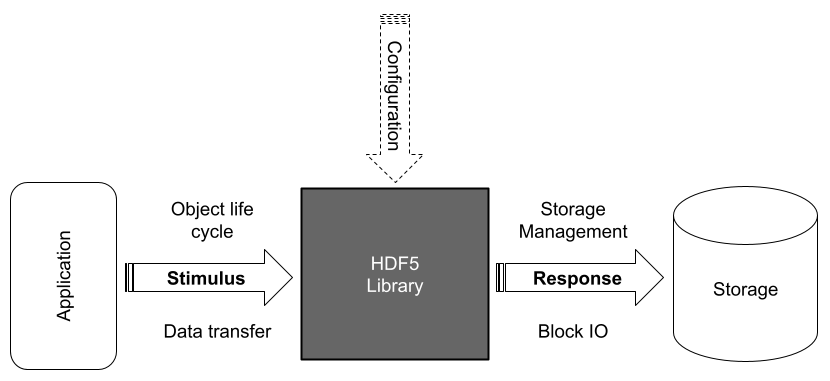
\includegraphics[width=0.9\textwidth]{images/Black box.png}
\caption{A black box model of the HDF5 library.}
\label{fig:blackbox}
\end{figure}

Despite its simplicity, a black box model gives us context for other models and lets us ask relevant questions. One of its central premises is that by correlating stimuli and responses, we might be able to draw certain conclusions about the black box's ``inner workings." However, it is not straightforward to correlate HDF5 API calls with actual IO activity. This is the case for three reasons:
\begin{enumerate}
    \item The HDF5 library is an intermediate abstraction layer
    \item It (de-)serializes collections of complex object constellations into storage structures
    \item IO activity occurs in blocks.
\end{enumerate}
Hence, we must open the box, which is what this document is about.

The stimuli to which we can subject the black box come in two forms: object life cycle management instructions and data transfer requests. Object life cycle management means tasks such as creating and modifying familiar HDF5 objects (datasets, groups, datatypes). By data transfer, we mean any kind of \texttt{*read*} or \texttt{*write*} API call, which is intended to transfer user (meta-)data into storage.

The black box responds to stimuli in two forms: storage management and block IO operations. Typical examples of storage include file systems and object stores. Specific responses depend on how HDF5 data model primitives are encoded in storage primitives. Examples include single- or multi-file layouts or collections of storage objects.

When observing the stimulus/response ``traffic" of even simple applications, the correlation is much weaker and less direct than we might expect and sometimes outright counter-intuitive (e.g., an input operation triggering an output operation). Unlike a mathematical function, which consistently produces the same outputs for the same inputs, the relation between stimuli and responses exhibited by the HDF5 library is non-functional, albeit deterministic. This is due to the HDF5 library's role as a translator between HDF5 model idioms, represented in memory, and storage idioms. To be effective and efficient, and to bridge the speed differential between memory and storage, the HDF5 library maintains a state. This state dilutes the simple stimulus/response logic and manifests itself in what might appear as a delayed response or an aggregate response to a sequence of stimuli.

The architecture of a system or software is usually presented in models that fall under different perspectives or views, such as the ones shown in table~\ref{table:perspectives}.

\begin{table}[h!]
\begin{tabular}{||c|l||}
\hline
Perspective or View & Description \\  [0.5ex] 
\hline\hline
Purpose/objective & What the client wants \\  
Form & What the system is \\
Behavioral or functional & What the system does\\
Performance objectives or requirements & How effectively the system does it\\
Data & The information retained in the system and its relationships\\
Managerial & The process by which the system is constructed and managed\\ [1ex] 
\hline
\end{tabular}
\caption{Six common perspectives or views.~\cite{maier2009}}
\label{table:perspectives}
\end{table}

For a given system or software, not all of them are equally important or relevant at all times. For example, the library build process and testing (managerial view) is covered in the first guided tour, whereas the modular library structure (functional view) is the organizing principle for the reference.

\section{Purpose, Objectives, and Values}

The purpose of the \acrshort{hdf5} library is to ensure efficient and equitable access to science and engineering data stored in HDF5 files across platforms and environments, now and forever. Toward that purpose, the two main objectives are:

\begin{enumerate}
    \item Self-describing data
    \item Portable encapsulation and access
\end{enumerate}

Self-describing data captures all information about itself necessary to reproduce and interpret it as intended by its producer. A storage representation must preserve the self-describing nature when transferring such representations over a network or to different storage. At the same time, it should be accompanied by a portable library that allows applications to access the data without knowing anything about the details of the representation.

The ``marriage''~\cite{kuehn1996} of the HDF5 file format and library is a specific implementation of the primitives and operations defined by the HDF5 data model and was adapted for several specific use cases over time.

\begin{figure}[ht]
\centering
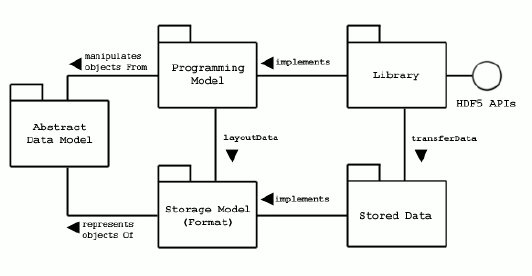
\includegraphics[width=0.7\textwidth]{images/models.png}
\label{fig:img1}
\caption{Models}
\end{figure}

The implementation is guided by the following values, which are listed in no particular order.

\begin{description}
    \item[Extensibility] The degree to which users can change behavior and appearance.
    \begin{itemize}
        \item Datatypes, conversions
        \item Filters
        \item Links
        \item Data virtualization
        \item Storage types
        \item File format micro-versioning
    \end{itemize}
    \item[Compatibility, Longevity, \& Stability] Things that worked before continue to work the same indefinitely
    \begin{itemize}
        \item Quasi-static data model
        \item Backward- and forward compatibility
        \item API Versioning
        \item Open file format specification
    \end{itemize}
    \item[Efficiency] Effective operation as measured by comparing production with cost (as in time, storage, energy, etc.)
    \begin{itemize}
        \item Algorithmic complexity
        \item Scalability
    \end{itemize}
    \item[Maintainability] The degree to which it can be modified without introducing fault
    \begin{itemize}
        \item Additive software construction~\cite{hanson2021}
    \end{itemize}
    \item[Progressiveness] A measure of eagerness to make progress and leverage modern storage technology
    \item[Freedom] Specifically, free software means users have the four essential freedoms~\cite{fsf2023}
    \begin{itemize}
        \item The freedom to run the program as you wish, for any purpose (freedom 0).
        \item The freedom to study how the program works, and change it so it does your computing as you wish (freedom 1). Access to the source code is a precondition for this.
        \item The freedom to redistribute copies to help others (freedom 2).
        \item The freedom to distribute copies of your modified versions to others (freedom 3). By doing this, you can give the whole community a chance to benefit from your changes. Access to the source code is a precondition for this.
    \end{itemize}
\end{description}

\section{Typographic conventions}

\begin{itemize}
    \item[\textbf{bold}] headers, titles
    \item[\textit{italic}] emphasis
    \item[\texttt{monospace}] Source code, package names, configuration file settings, file system paths and folder names.
\end{itemize}

\chapter{Guided Tours}\label{part:tours}
%|  Name  | TODO | ONGOING | DONE |
%|--------|------|---------|------|
%| Dana   | x    |         |      |
%| Gerd   |      |         |  X   |
%| Glenn  |      |         |  x   |
%| Jordan | x    |         |      |
%| Luke   | x    |         |      |
%| Matt   |      |         |  x   |
%| Neil   | x    |         |      |
%| Scot   | x    |         |      |

These guided tours introduce certain architectural elements in a specific context, and the level of detail is calibrated to the context. Complete coverage of the architectural concepts is provided in Chapter~\ref{part:reference}.

A simple program typically sets the course of a specific guided tour, and the call stack is the starting point for ``HDF5 library stratigraphy.'' We will examine how changes in the program change the call stack and activate and exercise different parts of the library. We hope the samples extracted from several well-placed ``stratigraphic test wells'' will create a reasonably accurate and complete picture of the library's modular structure and functional allocation.


\section{Meet the HDF5 library}\label{chap:hdf5-lib}

%|  Name  | TODO | ONGOING | DONE |
%|--------|------|---------|------|
%| Dana   | x    |         |      |
%| Gerd   |      |         | x    |
%| Glenn  |      |         |  x   |
%| Jordan | x    |         |      |
%| Luke   | x    |         |      |
%| Matt   |      |         | x    |
%| Neil   | x    |         |      |
%| Scot   | x    |         | x     |


%CLEANUP \todo[inline]{Owner: Gerd -- Priority: High -- Effort: S -- Completion: 100\%}

Throughout this tour, we describe the run-time use of the term `HDF5 library', which provides complete coverage of the architectural concepts in different contexts with different meanings. It should be clear from the context which meaning is intended, but we list them here for completeness. The term `HDF5 library' refers to one of the following:

\begin{enumerate}
    \item An architectural concept.
    \item A body of source code, versions of which can be found on GitHub~\cite{libhdf52023}.
    \item A binary compiled and configured for a particular platform using CMake~\cite{cmake2023} or Autotools~\cite{autotools2023}.
    \item An HDF5 library binary loaded into the context of a process, a library \textit{instance}.
    \item The internal state of an HDF5 library instance.
    \item A combination of one or more of the above, in a generic sense.
\end{enumerate}

We begin with a 35,000-foot overview of how the HDF5 library is structured. As shown in Figure~\ref{fig:vol-arch}, \textit{the primary purpose of the HDF5 library is to provide mappings between in-memory representations of HDF5 objects or entities and storage representations}. There are many possible implementations of such mappings, all of which share the HDF5 data model and library API. The API comprises two types of functions: functions dealing with the management of virtual objects and functions configuring API behavior or virtual object support functions. In Figure~\ref{fig:vol-arch}, this division is represented by the boxes labeled `Virtual Object Layer' and `Non-VOL API Calls.'

\begin{comment}
@startuml
participant Application as app
participant "HDF5 Library" as lib

group Explicit open/close
 app -> lib: H5open()
 rnote over lib: H5_init_library() \n- Phase 1 Modules \n- Phase 2 Modules

 app -> lib: H5close()
 rnote over lib: H5_term_library()

end
group Implicit open/close
 app -> lib: API Call / Symbol Evaluation
 rnote over lib: H5open()
 rnote over lib: H5_init_library() \n- Phase 1 Modules \n- Phase 2 Modules

 app -> lib: Application Exit Begins
 rnote over lib: H5close()
 rnote over lib: H5_term_library()
 lib -> app: HDF5 Library Exit Complete
 rnote over app: Application Exit Complete
end
@enduml
\end{comment}

\begin{figure}[h]
\centering
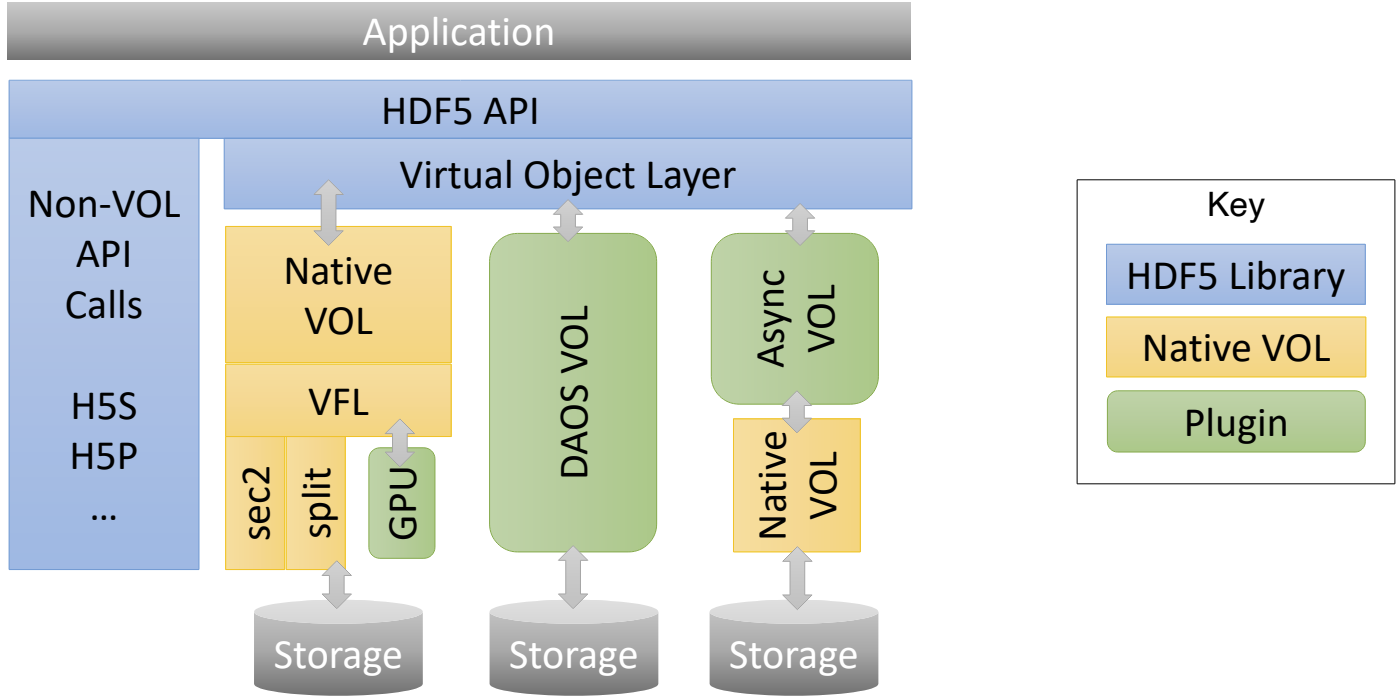
\includegraphics[width=0.7\textwidth]{images/VOL_arch.png}
\caption{The VOL architecture.}
\label{fig:vol-arch}
\end{figure}

The Virtual Object Layer (VOL) is an HDF5 library extension interface for implementing actual mappings of virtual objects to storage and implementing the operations associated with such objects' life cycle (creation, deletion, copying, etc.). Modules implementing such mappings are called VOL \textit{connectors} and are typically packaged as dynamically loadable plugins. In Figure~\ref{fig:vol-arch}, three VOL connector examples are shown: the so-called `Native VOL', the DAOS VOL~\cite{soumagne2021}, and the Async VOL~\cite{tang2020}. Notice that certain VOL connectors are stackable and that the native VOL is \textit{not} implemented as a plugin. The latter is due to the VOL-centric library architecture being relatively new. It was introduced in HDF5 library release 1.12.0 and underwent a significant revision for the HDF5 1.14.0 release. Before introducing the VOL layer, the HDF5 library was more or less identical to the native VOL connector (plus the non-VOL support functions). Perhaps the main takeaway from Figure~\ref{fig:vol-arch} is that what's now considered the HDF5 library is a lot smaller than expected. Today, the HDF5 library consists of an API, the VOL interface, and a non-VOL API management infrastructure. Of course, that bare-bones library doesn't do anything useful, and we need at least one VOL connector that implements an actual mapping of HDF5 virtual objects to storage.

Since, during this tour, we only examine library initialization and finalization, we will not encounter any ``proper" VOL functions. No virtual objects are constructed or mapped to storage, and no operations are performed on them. We will witness the initialization and finalization of the library's non-VOL infrastructure and the native VOL packages. During subsequent tours, we will see the native VOL in action, i.e., mapping HDF5 virtual objects to files formatted according to the HDF5 file format specification~\cite{ffmt} via the native VOL's Virtual File Layer (VFL) extension interface.

Unless stated otherwise and to keep the discussion simple, in this chapter, we include the native VOL connector when we refer to the HDF5 library. As we saw, however, this is not entirely true.

In this section, we describe the life cycle of an HDF5 library instance running in the context of an application process. This includes lazy library initialization, dynamic configuration, and finalization. At the end of this section, the reader should have enough information to answer the following questions:

\begin{itemize}
    \item What does it mean for a library instance to be initialized/finalized?
    \item What triggers a library instance initialization/finalization?
    \item What's the sequencing of library initialization/finalization?
    \item As a library developer, what library changes require careful consideration of/coordination with library initialization/finalization?
\end{itemize}

\paragraph{Prototype.} Consider the HDF5 version of a ``Hello, World!" program shown in Listing~\ref{lst:explicit-init}. The naming \func{H5[open,close]} is perhaps a little misleading (Why not \func{H5[init,finalize]}?), but, for reasons which will become clear later, most users and developers will never call these two functions directly.

\begin{listing}[H]
\caption{Explicit HDF5 library run-time initialization and finalization.}
\label{lst:explicit-init}
\begin{minted}[linenos]{C}
#include "common.h"
int main() {
    H5open();
    printf("Hello, HDF5!\n");
    H5close();
    return 0;
}
\end{minted}
\end{listing}


\paragraph{Goals.} The main goals of library initialization and finalization are:

\begin{itemize}
    \item Setup and tear-down of error handling infrastructure
    \item Module initialization and finalization, including
    \begin{itemize}
        \item (De-)Registration of API entity types (or classes)
        \item Initialization and finalization of global variables
        \item Retrieval of environment variables, e.g., for the discovery of plugin paths
    \end{itemize}
\end{itemize}

\paragraph{Control flow.} A cursory inspection of the call graph of the program shown in Listing~\ref{lst:explicit-init} suggests that \func{H5[open,close]} proceed directly to \func{H5_[init,term]_library}, respectively.

\func{H5_init_library} is responsible for calling the initializers of all non-VOL and native VOL library modules (aka ``packages") in the correct order so that no module is initialized before its prerequisite modules. A table in \func{H5_init_library} establishes the order of initialization. The table, as implemented at the time of this writing, is shown in Listing~\ref{lst:init-table}.

\begin{listing}
\centering
\caption{\func{H5_init_library} initialization table.}
\label{lst:init-table}
\begin{minted}[linenos]{C}
struct {
    herr_t (*func)(void);
    const char *descr;
} initializer[] = {
    {H5E_init, "error"}
,   {H5VL_init_phase1, "VOL"}
,   {H5SL_init, "skip lists"}
,   {H5FD_init, "VFD"}
,   {H5_default_vfd_init, "default VFD"}
,   {H5P_init_phase1, "property list"}
,   {H5AC_init, "metadata caching"}
,   {H5L_init, "link"}
,   {H5S_init, "dataspace"}
,   {H5PL_init, "plugins"}
/* Finish initializing interfaces that depend on the interfaces above */
,   {H5P_init_phase2, "property list"}
,   {H5VL_init_phase2, "VOL"}
};
\end{minted}
\end{listing}

Most package initializers (the \texttt{H5*\_init*} routines) register identifier classes or check environment variables. The only notable exception is the \texttt{H5T} package initializer, which initializes identifiers (stored in global variables) for built-in datatypes and several pre-defined datatype transformations. For this tour, where we do not encounter any identifiers, it is sufficient to know that identifiers are ephemeral handles of API type \texttt{hid\_t}, which the library uses to track API entities. For efficiency and error checking, the identifier space is ``partitioned'' into identifiers of different types, and developers can create (register) custom identifier types to track their entities.

As the table shows, a few modules (\texttt{H5P,H5VL}) require phased initialization. \texttt{H5\_default\_vfd\_init()}, in connection with \texttt{H5P\_init\_phase2()},  registers and initializes the POSIX VFD as the default file driver. Finally, \texttt{H5VL\_init\_phase2()} initializes the remaining modules according to a similar table shown in Listing~\ref{lst:vol2-init-table}.

\begin{listing}
\centering
\caption{\func{H5VL_init_phase2} initialization table.}
\label{lst:vol2-init-table}
\begin{minted}[linenos]{C}
struct {
    herr_t (*func)(void);
    const char *descr;
} initializer[] = {
    {H5T_init, "datatype"}
,   {H5O_init, "object header"}
,   {H5D_init, "dataset"}
,   {H5F_init, "file"}
,   {H5G_init, "group"}
,   {H5A_init, "attribute"}
,   {H5M_init, "map"}
,   {H5CX_init, "context"}
,   {H5ES_init, "event set"}
,   {H5Z_init, "transform"}
,   {H5R_init, "reference"}
};
\end{minted}
\end{listing}

\func{H5VL_init_phase2} concludes the HDF5 library initialization.

Only \texttt{H5[A,D,F,G,L,M,T]} API functions will pass through the VOL layer; all other packages support non-VOL API calls or library internal infrastructure.

\noindent\fbox{\parbox{\linewidth}{At this point, the library would be considered initialized with its default configuration (native VOL + POSIX VFD), and the application can proceed to create and manipulate HDF5 virtual objects that are mapped to HDF5 files in a POSIX-compliant file system. For other mappings, different VOL connectors or VFD plugins would be required.}}

The library has a default behavior to shut down when the application exits by registering an \texttt{atexit(3)} handler, \func{H5_term_library}. This will invoke modules' \func{H5*_[top]_term_package} functions. The shutdown table is too extensive to be repeated here. It is also heavily commented on and should be consulted for more in-depth information. Akin to the phased initialization for certain modules, the finalization of a few modules is split into ``top" and ``bottom" portions. Note that some entries in the shutdown table are marked as ``barriers," and if a new module should only be shutdown \textit{strictly after} the preceding modules, then it should be marked as a barrier. This is achieved by setting the \texttt{wait} parameter of the \texttt{TERMINATOR} macro for the corresponding module to \texttt{true}.

\paragraph{Data flow.} The library's initialization and finalization state are tracked in two global variables, namely \texttt{H5\_INIT\_GLOBAL} and \texttt{H5\_TERM\_GLOBAL}. These variables are specifically set by two library functions \texttt{H5\_init\_library()} and \texttt{H5\_term\_library()}, respectively. The initialization and finalization of library modules typically involve registering and unregistering module-specific identifier types (for example, \texttt{H5I\_DATASPACE\_CLS} and \texttt{H5I\_SPACE\_SEL\_ITER\_CLS} for \texttt{H5S}) and the initialization/finalization of module-specific global variables. Perhaps the most elaborate example is \texttt{H5T}, which requires the initialization/finalization of built-in datatypes such as \texttt{H5T\_IEEE\_F64BE\_g} and conversion functions such as \texttt{H5T\_\_conv\_double\_ldouble()} in the global variable \texttt{H5T\_g}. Otherwise, there is very little data flow activity during library initialization/finalization.

\begin{listing}
\centering
\caption{Implicit HDF5 library initialization.}
\label{lst:implicit-init}
\begin{minted}[linenos]{C}
#include "common.h"
int main() {
  unsigned int majnum, minnum, relnum;
  H5get_libversion(&majnum, &minnum, &relnum);
  printf("Hello, HDF5 %u.%u.%u!\n", majnum, minnum, relnum);
  return 0;
}
\end{minted}
\end{listing}

\paragraph{Variants.} In Listing~\ref{lst:implicit-init}, a variant of the ``Hello, World!" example is shown. The notable difference is the new function \func{H5get_libversion}, while the previous version had calls to \func{H5open} and \func{H5close}, which have been removed in the new version. It turns out that the HDF5 library initializes itself as needed whenever an application either enters the library through an API function call such as \func{H5get_libversion}, or when an application evaluates an HDF5 symbol that represents a macro such as \texttt{H5F\_ACC\_RDONLY} or \texttt{H5F\_ACC\_RDWR}, a property-list class identifier such as \texttt{H5P\_FILE\_ACCESS}, a VFD identifier such as \texttt{H5FD\_FAMILY} or \texttt{H5FD\_SEC2}, or a type identifier
such as \texttt{H5T\_NATIVE\_INT64}.

The library provides a couple of macros that initialize the library as necessary. Library initialization is checked as a side-effect of the \texttt{FUNC\_ENTER\_API*} macros used at the top of most API functions. HDF5 library symbols other than functions are provided through \texttt{\#define}s that use the \texttt{H5OPEN} macro to introduce a library-initialization call (\texttt{H5open()}) at each site where a non-function symbol is used.

Two noteworthy variants of HDF5 library initialization and finalization will be discussed in later tours. One is the case of MPI-parallel HDF5
%(see section~\ref{sec:MPI-state-n-sync})
, where multiple library instances simultaneously operate on one or more files with different sharing patterns. The other one is the use case of a library built with thread-safety enabled  (see section~\ref{sec:H5TS-impl}). In both cases, the changes to HDF5 library initialization and finalization are ``around the edges" and deal with MPI initialization, finalization, and API lock management, respectively.



\paragraph{Developer considerations.} When a developer exports a new symbol as part of the HDF5 library, they should ensure that an application cannot enter the library in an uninitialized state through a new API function or read an uninitialized value from a non-function HDF5 symbol.

If a developer adds a module to the library that must be initialized with the rest of the library, then they should insert its initializer into the right place in the table.

If a developer adds a module that needs to release resources during library shutdown, they should add a call to the shutdown table at the right place.

\paragraph{Source code recommended for study.}

\begin{itemize}
    \item \func{H5_[init,term]_library} in \texttt{H5.c}
    \item \func{H5E_[init,term]_package} in \texttt{H5E.c}
    \item \func{H5T_init, H5T_top_term_package} in \texttt{H5T.c}
    \item \func{H5VL_init_phase2} in \texttt{H5VLint.c}
\end{itemize}

\subsection{Summary}

\begin{figure}[h]
\centering
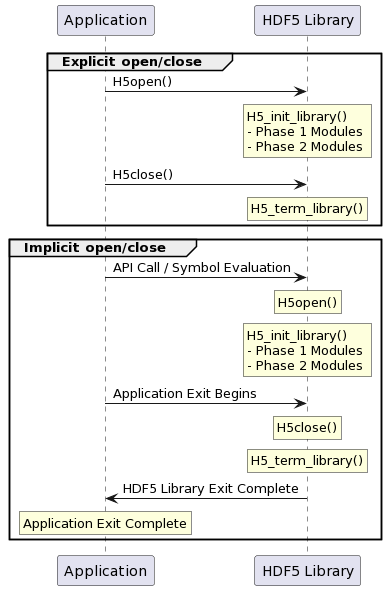
\includegraphics[width=0.5\textwidth]{images/tour_1_uml.png}
\label{fig:tour-1-uml}
\caption{Library initialization/termination sequence diagram.}
\end{figure}

Given the substantial library infrastructure we have seen during this tour, it is too easy to ``miss the architecture for the code". The key takeaway from this tour is that, as suggested in Figure ~\ref{fig:vol-arch}, the HDF5 library consists of
\begin{enumerate}
    \item A (C-) API
    \item An extension interface (VOL) to implement mappings between HDF5 virtual objects and storage representations
    \item A supporting infrastructure (non-VOL) for API handle management, API properties, etc.
    \item A default mapping (native VOL) between HDF5 virtual objects and the content of files formatted according to the HDF5 file format specification~\cite{ffmt}.
\end{enumerate}

Library initialization and finalization are usually triggered by API entry and an \texttt{atexit(3)} handler. The HDF5 library source code is organized modularly, and initialization and finalization proceed through modules in a defined order, respecting inter-module dependence. Developers must guard against uncontrolled API entrance, violations of module interdependence during library initialization and shutdown, and failures to release unused resources.


\section{The life cycle of HDF5 files}\label{sec:tour2}

%|  Name  | TODO | ONGOING | DONE |
%|--------|------|---------|------|
%| Dana   | x    |         |      |
%| Gerd   |      |         | x    |
%| Glenn  | v    |         |   x  |
%| Jordan | x    |         |      |
%| Luke   | x    |         |      |
%| Matt   |      |         |  x   |
%| Neil   | x    |         |      |
%| Scot   | x    |         |   x   |

%CLEANUP \todo[inline]{Owner: Gerd -- Priority: High -- Effort: M -- Completion: 100\%}

Throughout this tour, we describe the life cycle of HDF5 files.

\paragraph{Terminology.} As we saw in the previous tour (Section~\ref{chap:hdf5-lib}), the term ``HDF5 library" has several context-dependent meanings. Likewise, the term `HDF5 file' refers to one of the following:

\begin{enumerate}
    \item A kind of HDF5 virtual object.
    \item A portion of the HDF5 library that represents an open HDF5 file.
    \item A terminal VOL connector-specific in-storage representation, including ``file-less."
    \item One or more files stored in a file system or object store formatted according to the HDF5 file format specification~\cite{ffmt}.
    \item A combination of one or more of the above, in a generic sense.
\end{enumerate}

We first describe an HDF5 file’s runtime life cycle before covering a few finer points in subsequent sections.

\subsection{Life cycle}

In this section, we describe the internals of an HDF5 file's life cycle, including VOL connector and VFD selection and handling, by reviewing the \texttt{H5Fcreate(), H5Fopen(),} and \texttt{H5Fclose()} stacks. At the end of this section, the reader should have enough information to answer the following questions:

\begin{itemize}
    \item How do HDF5 library API calls get ``routed" through the VOL layer?
    \item Under what circumstances do they enter the native VOL connector?
    \item How are HDF5 files represented in memory?
    \item What is the HDF5 virtual file layer (VFL), and how does it relate to the rest of the HDF5 library?
    \item How does the HDF5 library select virtual file drivers (VFD)?
\end{itemize}

\paragraph{Prototype.} Let's consider the simplest program to create a new HDF5 file shown in Listing~\ref{lst:file-101}.

\begin{listing}
\centering
\caption{An ``empty'' (800 B) HDF5 file.}
\label{lst:file-101}
\begin{minted}[linenos]{C}
#include "common.h"
int main() {
    hid_t file_id = H5Fcreate("hello.h5", H5F_ACC_TRUNC, H5P_DEFAULTx2);
    H5Fflush(file_id, H5F_SCOPE_GLOBAL);
    size_t size;
    H5Fget_filesize(file_id, &size);
    printf("File size: %zu\n", size);
    H5Fclose(file_id);
    return 0;
}
\end{minted}
\end{listing}

We create an ``empty" HDF5 file. Of course, such a minimal HDF5 file must contain a root group! Finally, we print its in-storage size. (As we will see later, the call to \texttt{H5Fflush()} is necessary to get an accurate size.)

\paragraph{Goals.} The main goals of the HDF5 file creation/open/close life cycle are:
\begin{itemize}
    \item Create an in-memory representation of an HDF5 file.
    \item Return a file identifier or handle (\texttt{hid\_t}) to the caller.
    \item Serialize and persist the file object in storage.
    \item Free all resources associated with the file upon closure of the last handle.
\end{itemize}

\paragraph{Control flow.} As we saw in Section~\ref{chap:hdf5-lib}, any API call, in this case, \texttt{H5Fcreate()}, will trigger library initialization, which includes the registration of the native VOL as the default VOL connector and the POSIX VFD (sec2) as the default file driver. 

The call sequence for each API routine used in Listing~\ref{lst:file-101} may be found in Figures: ~\ref{fig:tour2-file-create} (\texttt{H5Fcreate()}), \ref{fig:tour2-file-flush} (\func{H5Fflush}), \ref{fig:tour2-file-get-filesize} (\func{H5Fget_filesize}), and ~\ref{fig:tour2-file-close} (\func{H5Fclose}). For modules whose API functions are routed through the VOL layer, we have adopted the notion of top and bottom portions, e.g., \texttt{H5F Top} and \texttt{H5F Bot.} Since the HDF5 library modules predate the introduction of the VOL layer, the code is not neatly separated into VOL handling/native VOL code portions. We refer to a module's VOL handling code portions as the module's `top' portion and the native VOL portion as the module's `bottom.'

\func{H5Fcreate} enters the VOL layer at \func{H5VL_file_create} via \texttt{H5F\_\_create\_api\_common()}. This routine handles sanity checking and calling the internal VOL layer routine, \texttt{H5VL\_file\_create()}. The native VOL connector is selected, and its file creation callback, \texttt{H5VL\_\_native\_file\_create()}, is invoked. The open routine from the file module, \texttt{H5F\_open()}, does all the heavy lifting in terms of allocation and initialization of various in-memory structures (see the section on data flow), creates a metadata cache for the file under construction (\texttt{H5AC\_create()}), and culminates in file superblock and root group creation.

On the following line, \texttt{H5Fflush()} is routed through the VOL layer via \texttt{H5F\_\_flush\_api\_common()}, which invokes the \texttt{H5VL\_file\_specific()} callback with operation type \texttt{H5VL\_FILE\_FLUSH}. The flush operation is handled by the native VOL's \texttt{H5VL\_\_native\_file\_specific()}.

Similarly, the call to \texttt{H5Fget\_filesize()} is routed through the VOL layer's \texttt{H5VL\_file\_optional()} callback with the operation type \texttt{H5VL\_NATIVE\_FILE\_GET\_SIZE}, eventually reaching the native VOL's implementation of the get filesize operation within \texttt{H5VL\_\_native\_file\_optional()}. This invokes the native VOL's internal \texttt{H5F\_\_get\_max\_eof\_eoa()}, which invokes the VFL's \texttt{H5FD\_get\_eo[a,f]()} and adds them to the file's base address obtained from \texttt{H5FD\_get\_base\_addr()}.

\texttt{H5Fclose()} proceeds to decrement the file ID's reference count via \texttt{H5I\_dec\_app\_ref()}. If the reference count has reached 1, which it has in this example, this triggers the invocation of the free function for the particular identifier type, a file ID (\texttt{H5I\_FILE}), in this case. The free function in this case is \texttt{H5F\_\_close\_cb()} via which we re-enter the VOL through \texttt{H5VL\_file\_close()}, which in turn calls the native VOL's \texttt{H5VL\_\_native\_file\_close()}. This triggers the release of in-memory file resources, including flushing and destroying the file-specific metadata cache, via \texttt{H5F\_\_dest()}.

\begin{comment} 
http://www.plantuml.com/plantuml/uml/
@startuml

participant "H5F Top" as H5Ft
participant H5VL as H5VL
participant "Native VOL" as native
participant "H5F Bot." as H5Fb

rnote over H5Ft: H5Fcreate
H5Ft -> H5VL: H5F__create_api_common
H5VL -> native: H5VL_file_create
native -> H5Fb: H5VL__native_file_create
H5Fb -> H5AC: H5F__open
rnote over H5AC: H5AC_create
rnote over H5Fb: H5F__super_init
participant "H5G Bot." as H5Gb
H5Fb -> H5Gb: H5G_mkroot

@enduml
\end{comment}

\begin{figure}
    \centering
    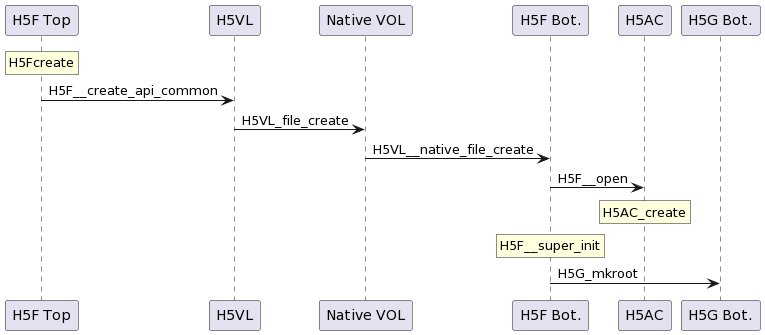
\includegraphics[width=0.80\textwidth]{images/tour2_file_create.png}
    \caption{File creation sequence diagram}
    \label{fig:tour2-file-create}
\end{figure}

\begin{comment}
http://www.plantuml.com/plantuml/uml/
@startuml

participant "H5F Top" as H5Ft
participant H5VL as H5VL
participant "Native VOL" as native
participant "H5F Bot." as H5Fb

rnote over H5Ft: H5Fflush
H5Ft -> H5VL: H5F__flush_api_common
H5VL -> native: H5VL_file_specific
native -> H5Fb: H5VL__native_file_specific
alt Global flush
rnote over H5Fb: H5F_flush_mounts
else Local flush
rnote over H5Fb: H5F_flush
end

@enduml
\end{comment}

\begin{figure}
    \centering
    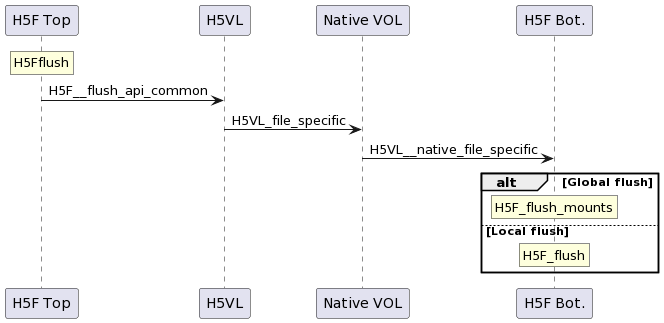
\includegraphics[width=0.7\textwidth]{images/tour2-file-flush.png}
    \caption{File flush sequence diagram}
    \label{fig:tour2-file-flush}
\end{figure}

\begin{comment}
http://www.plantuml.com/plantuml/uml/
@startuml
participant "H5F Top" as H5Ft
participant H5VL as H5VL
participant "Native VOL" as native
participant "H5F Bot." as H5Fb
participant H5FD
participant "sec2 Driver" as sec2

H5Ft -> H5VL: H5Fget_filesize
H5VL -> native: H5VL_file_otional
native -> H5Fb: H5VL__native_file_optional
H5Fb -> H5FD: H5F__get_max_eof_eoa
H5FD -> sec2: H5FD_get_eo[a,f]
rnote over sec2: H5FD__sec2_get_eo[a,f]
@enduml
\end{comment}

\begin{figure}
    \centering
    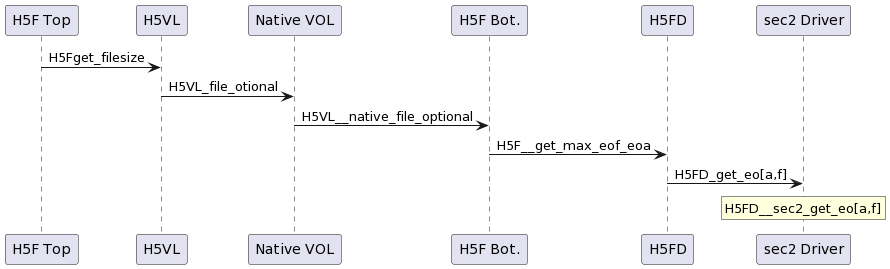
\includegraphics[width=0.95\textwidth]{images/tour2-file-get-filesize.png}
    \caption{Get filesize sequence diagram}
    \label{fig:tour2-file-get-filesize}
\end{figure}

\begin{comment}
http://www.plantuml.com/plantuml/uml/
@startuml
participant "H5F Top" as H5Ft
participant H5I as H5I
participant H5VL as H5VL
participant "Native VOL" as native
participant "H5F Bot." as H5Fb

H5Ft -> H5I:  H5Fclose
H5I -> H5Ft: H5I_dec_app_ref
H5Ft -> H5VL: H5F__close_cb
H5VL -> native: H5VL_file_close
native -> H5Fb: H5VL__native_file_close
rnote over H5Fb: H5F__dest
@enduml
\end{comment}

\begin{figure}
    \centering
    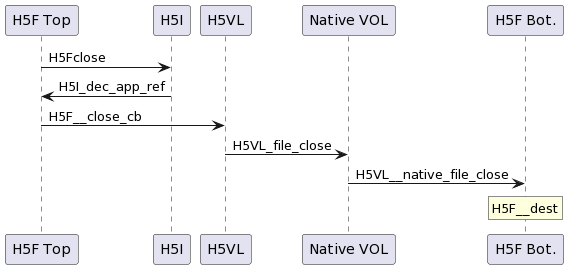
\includegraphics[width=0.70\textwidth]{images/tour2-file-close.png}
    \caption{File close sequence diagram}
    \label{fig:tour2-file-close}
\end{figure}

\begin{comment}
@startuml

participant Application as app
participant "H5F Top" as H5Ft
participant H5VL as H5VL
participant "Native VOL" as native
participant "H5F Bot." as H5Fb

app -> H5Ft: H5Fcreate
H5Ft -> H5Ft: H5F__create_api_common
H5Ft -> H5VL: H5VL_file_create
H5VL -> native: H5VL__native_file_create
native -> H5Fb: H5F__open
H5Fb -> H5AC: H5AC_create
H5Fb -> H5Fb: H5F__super_init
participant "H5G Bot." as H5Gb
H5Fb -> H5Gb: H5G_mkroot

app -> H5Ft: H5Fflush
H5Ft -> H5Ft: H5F__flush_api_common
H5Ft -> H5VL: H5VL_file_specific
H5VL -> native: H5VL__native_file_specific

app -> H5Ft: H5Fget_filesize
H5Ft -> H5VL: H5VL_file_otional
H5VL -> native: H5VL__native_file_optional
native -> H5Fb: H5F__get_max_eof_eoa
participant H5FD as H5FD
H5Fb -> H5FD: H5FD_get_eo[a,f]

app -> H5Ft: H5Fclose
participant H5I as H5I
H5Ft -> H5I: H5I_dec_app_ref
H5I -> H5Ft: H5F__close_cb
H5Ft -> H5VL: H5VL_file_close
H5VL -> native: H5VL__native_file_close
native -> H5Fb: H5F__dest

@enduml
\end{comment}

%\begin{figure}
%\centering
%\includegraphics[width=1\textwidth]%{images/tour_2_file_creation_and_size_retrieval.png}
%\caption{File creation and size retrieval sequence diagram.}
%label{fig:tour-2-uml-1}
%\end{figure}

Before looking at variants of this control flow, we look at the data flow and provide the ``Cliff notes" for the VOL and VFL layers. A detailed architectural overview can be found in Section~\ref{ref:vol}.

\paragraph{Data flow.} Every time \texttt{H5F[create,open]()} is called, a structure of type \texttt{H5F\_t} (see Listing~\ref{lst:file-top}) is allocated.

\begin{listing}
\centering
\caption{A top-level file descriptor.}
\label{lst:file-top}
\begin{minted}[linenos]{C}
struct H5F_t {
    char          *open_name;
    char          *actual_name;
    H5F_shared_t  *shared;
    H5VL_object_t *vol_obj;
    unsigned       nopen_objs;
    H5FO_t        *obj_count;
    bool           id_exists;
    bool           closing;
    struct H5F_t  *parent;
    unsigned       nmounts;
};
\end{minted}
\end{listing}

Since HDF5 files can be opened multiple times with different \texttt{hid\_t} handles in the same process, the in-memory file representation is split into \texttt{H5open()} instance-specific top (\texttt{H5F\_t}) and shared bottom portions of type \texttt{H5F\_shared\_t}. Both \texttt{H5F\_t} and \texttt{H5F\_shared\_t} are defined in \texttt{H5Fpkg.h}. \texttt{H5F\_shared\_t} is too extensive to be reproduced here, but it contains all the information that is common among \texttt{H5Fopen()} instances, including:

 \begin{itemize}
     \item VOL connector and VFD information
     \item The metadata cache for this file and its configuration
     \item Version information
     \item Open HDF5 objects in the file
     \item File space management configuration
     \item Various status information.
 \end{itemize}
We strongly encourage the reader to review the well-documented \texttt{H5F\_shared\_t} definition!
 
Notice that most fields in \texttt{H5F\_shared\_t} show the file system heritage and represent information related to persisting HDF5 files in a file system according to the file format specification~\cite{ffmt}. For example, the \texttt{sblock} field of \texttt{H5F\_shared\_t} (see Listing~\ref{lst:file-sblock}) matches almost verbatim the file format specification.

\begin{listing}
\centering
\caption{File superblock in-memory representation.}
\label{lst:file-sblock}
\begin{minted}[linenos]{C}
typedef struct H5F_super_t {
    H5AC_info_t cache_info;
    unsigned    super_vers;
    uint8_t     sizeof_addr;
    uint8_t     sizeof_size;
    uint8_t     status_flags;
    unsigned    sym_leaf_k;
    unsigned    btree_k[H5B_NUM_BTREE_ID];
    haddr_t     base_addr;
    haddr_t     ext_addr;
    haddr_t     driver_addr;
    haddr_t     root_addr;
    H5G_entry_t *root_ent;
} H5F_super_t;
\end{minted}
\end{listing}

This is our first time encountering the metadata cache (\texttt{H5AC} module). For now, it is essential to remember that there is one metadata cache instance for each HDF5 file in the sense of \texttt{H5F\_shared\_t}, and \texttt{H5F\_super\_t} is its first protected entry.

Until this point, everything happened in memory, and no ``real" I/O has occurred. Considering the overhead associated with frequent small I/O operations, this behavior is quite desirable. Ignoring ``raw" data I/O, metadata, such as the file superblock, will be written only on flush events, or when an HDF5 file (\texttt{H5F\_shared\_t}) is closed, and the associated metadata cache instance is destroyed (see \texttt{H5F\_\_dest()}). Speaking roughly, metadata I/O happens less frequently as the direct consequence of API calls than as the result of metadata cache events, such as entry evictions.

The downside of this apparent de-correlation of in-memory metadata management and I/O adds a certain fragility to the state of an HDF5 file that's open in a modifying access mode. If an application terminates unexpectedly, the library may not get to persist modified portions of the file state. Future implementations might offer better protection against file corruption.

It is hard to overstate the central role of the metadata cache's role in the HDF5 native VOL, although that might not yet be apparent. We will have more to say about the metadata cache in subsequent tours.

\subsection{Detour: The Virtual Object Layer}\label{sec:vol}

\paragraph{Goals} The purpose of the Virtual Object Layer (VOL) is to decouple the HDF5 library's API and object abstractions from a particular storage implementation while requiring minimal change in how the API is used. It allows for independent, potentially user-defined VOL connectors to handle virtual object operations. A common use case for VOL connectors is to change how HDF5 files are stored, mapping an HDF5 file in memory to something other than a POSIX file in storage - for example, a collection of objects in an AWS S3 bucket. The VOL layer's capabilities are more general than just changing the implementation of storage - a connector can perform arbitrary operations (such as logging, caching, or mirroring) whenever a routine that is part of the VOL API is used.

\paragraph{VOL Architecture}  Figure~\ref{fig:vol-arch} shows how the VOL fits into the library's structure. Operations that deal with storage or virtual objects are part of the VOL API, which means that calls pass through one or more VOL connectors before reaching storage. There are two types of VOL connectors: pass-through connectors, which pass control flow to another connector after performing some operation, and terminal connectors, which do not pass on to another connector and are generally used to map objects to storage. 

Library functions which are a part of the VOL API internally call a function of the form \func{H5*__<operation>_api_common}, which routes the call to the VOL layer via \func{H5VL_<operation>}. The VOL layer determines which connector to use by checking the property list that was passed as an argument to the original API call.

For example, with the default file access property list (FAPL) specified by \texttt{H5P\_DEFAULT}, the top level \func{H5Fopen} internally calls \func{H5F__open_api_common}, which passes control to \func{H5VL_file_open}. Because the default FAPL specifies the native VOL connector, \func{H5VL_file_open} will invoke the native VOL's file open callback \func{H5F\_open} (note the underscore!), which opens an HDF5 file object from a locally-stored POSIX file. A VOL connector provides pointers to its callbacks in its \texttt{H5VL\_class\_t} struct. (See Section~\ref{ref:vol}.)

VOL connectors other than the native connector are distributed as plugins loaded into an application. There are three ways to load a connector: dynamic loading using environment variables, dynamic loading with API calls, and manual linking to the connector.

\paragraph{Dynamic Loading with Environment Variables} Dynamic loading with environment variables does not require rebuilding or modifying the application. However, it does not allow an application to load multiple VOL connectors.

At runtime, the library checks the environment variable \texttt{HDF5\_VOL\_CONNECTOR} for the name of a VOL connector to load. This name is case-sensitive and is specified manually by each connector - the DAOS VOL connector, for example, expects to be discovered under the name \texttt{daos}. 

If the VOL connector is not installed to a default system path, then the environment variable \texttt{HDF5\_PLUGIN\_PATH} must be used to specify the absolute path to the connector. Generally, this will be the \texttt{/lib} subdirectory of wherever the connector was installed.

If the VOL connector is successfully loaded through environment variables, the library's default property lists, accessed via the \texttt{H5P\_DEFAULT} macro, will tell the VOL layer to use the dynamically loaded connector.

\paragraph{Dynamic Loading via API calls} There are two methods to load a VOL connector as a plugin and assign it an \texttt{hid\_t} handle: \texttt{H5VL\_register\_by\_name()} and \texttt{H5VL\_register\_by\_value()}. When choosing to use \texttt{H5VL\_register\_by\_value()}, a VOL connector identifier needs to be provided, which is a unique number assigned to each registered VOL by the HDF Group.  On the other hand, \texttt{H5VL\_register\_by\_name()} is a method that generally requires the same name that would be provided to \texttt{HDF5\_VOL\_CONNECTOR}, although it may vary depending on the connector.

Once the connector has been registered and assigned an \texttt{hid\_t} handle, this handle may be provided to \texttt{H5Pset\_vol} to modify a FAPL, telling any VOL layer function that checks this FAPL to use the supplied connector.

\paragraph{Manual Linking} Linking a VOL connector requires modifying the source and build of the target application but provides more flexibility in how the connectors may be used. 

The requirements to link and use a connector are as follows:
\begin{itemize}
    \item Link to the connector's library at application build time
    \item Include the connector's public headers in the application
    \item Potentially invoke any initialization/termination functions of the connector at the start/end of the application
\end{itemize}

Once these requirements are satisfied, the FAPL is modified using  \texttt{H5Pset\_fapl\_<vol\_name>()} or \texttt{H5Pset\_<vol\_name>()} so that any VOL API calls provided with that FAPL will use the specified connector. Note that the exact function name for this operation will vary by connector in a way that does not adhere to any strict pattern.

\subsection{Detour: The Virtual File Layer}\label{sec:vfl}

A popular metaphor refers to HDF5 files as ``file systems in a file." The Virtual File Layer (VFL) adds some credibility to this metaphor. This section reviews the HDF5 Virtual File Layer, its requirements and assumptions, and its place in the library.

\paragraph{Overview} The VFL serves a purpose similar to the VOL -- outsourcing the implementation of specific storage-related operations to potentially user-defined Virtual File Drivers (VFDs) while minimizing the changes necessary in user applications. However, the scope of the VFL is narrower: it defines a mapping between the HDF5 address space and file system-like storage. 

As seen in Figure~\ref{fig:vol-arch}, the Virtual File Layer (VFL) sits at the bottom of the native VOL. It is a native VOL extension interface. If a non-native VOL is used, the VFL will be bypassed entirely. Just as the native VOL is the default VOL connector, the sec2 driver (or 'POSIX VFD') is the default VFD, which uses POSIX functions to perform unbuffered I/O (with respect to the HDF5 library) to a single file. (See Section~\ref{sec:H5PB} for a configuration in which the HDF5 library performs buffering.)

\paragraph{Using a VFD.} Unlike the VOL layer, which has only the native VOL built into the library, several VFDs are included with the library and can be enabled with build options. These include the MPI-IO VFD for parallel file access and the read-only S3 (ROS3) VFD, which allows read-only access to HDF5 files stored as objects in AWS S3 buckets.

The process of using a VFD that is not built with the library is similar to the process of using a manually linked VOL connector:
\begin{itemize}
    \item The VFD must be linked to the application at the application's build time
    \item The VFD's public headers must be included 
\end{itemize}

After meeting the necessary requirements, the VFD can be enabled by modifying the FAPL using either \texttt{H5Pset\_driver\_by\_name()} or \texttt{H5Pset\_driver\_by\_value()}. \texttt{H5Pset\_driver\_by\_name()} requires a case-sensitive name specific to each VFD, and \texttt{H5Pset\_driver\_by\_value()} requires a `driver value,' a unique number assigned to each VFD that is registered with The HDF Group.

Alternatively, each VFD should define a function with a name of the form \texttt{H5P\_set\_fapl\_<VFD\_name>()}, which also modifies a FAPL to specify the use of that VFD. Listing~\ref{lst:file-core-vfd} shows a function of this form being used to enable the core VFD, a VFD that manages HDF5 files as contiguous memory buffers and maps I/O operations to memory accesses.

\paragraph{VFL Architecture.} Recall from the section on VOL Architecture that the property list for an operation determines which VOL is used. If the native VOL is selected, the property list also contains information about which file driver to use. Continuing the earlier example, the top level \texttt{H5Fopen()} eventually calls the native VOL's \texttt{H5F\_open()}, which invokes the VFL's \texttt{H5FD\_open()}. This VFL function uses the 'open' callback of the active file driver, which for the default sec2 driver is \texttt{H5FD\_\_sec2\_open()}. This driver callback is where the actual work to open a file in memory is performed. 

Each file driver provides pointers to its callbacks in an \texttt{H5FD\_class\_t} struct. These callbacks are invoked by handler functions with names of the form \texttt{H5FD\_<operation>()} in the VFL layer. % See section~\ref{ref:vfl} for more information about the VFL.

\paragraph{Variants.} Signaling the presence of architecture (!), the two variants shown in Listings~\ref{lst:file-101-latest} and~\ref{lst:file-core-vfd} follow the same sequence that's shown in Figures~\ref{fig:tour2-file-create} through \ref{fig:tour2-file-close}. They diverge from the prototype (Listing~\ref{lst:file-101}) in only two minor technical details.

The code shown in Listing~\ref{lst:file-101-latest} will modify the default values of the \texttt{[low,high]\_bound} fields of the file's \texttt{H5F\_shared\_t} structure. This affects how certain file metadata is serialized (a process triggered by metadata cache events) if a newer file format specification offers better alternatives or a use case requires it.

\begin{listing}
\centering
\caption{A modern ``empty'' (195 B) HDF5 file.}
\label{lst:file-101-latest}
\begin{minted}[linenos]{C}
#include "common.h"
int main() {
    hid_t fapl_id = H5Pcreate(H5P_FILE_ACCESS);
    H5Pset_libver_bounds(fapl_id, H5F_LIBVER_LATEST, H5F_LIBVER_LATEST);
    hid_t file_id = H5Fcreate("my_file.h5", H5F_ACC_TRUNC, H5P_DEFAULT,
        fapl_id);
    H5Fflush(file_id, H5F_SCOPE_GLOBAL);
    size_t size;
    H5Fget_filesize(file_id, &size);
    printf("File size: %zu\n", size);
    H5Fclose(file_id);
    H5Pclose(fapl_id);
    return 0;
}
\end{minted}
\end{listing}

As described earlier, the code in Listing~\ref{lst:file-core-vfd} instructs the library to select a non-default VFD. This will update the \texttt{lf} field of the file's \texttt{H5F\_shared\_t} structure, which wraps the VFD-specific callbacks. In other words, only \texttt{H5FD\_*()} calls will be affected by this change.

\begin{listing}
\centering
\caption{Using a different VFD.}
\label{lst:file-core-vfd}
\begin{minted}[linenos]{C}
#include "common.h"
int main() {
    hid_t fapl_id = H5Pcreate(H5P_FILE_ACCESS);
    H5Pset_fapl_core(fapl_id, 4096, 1);
    hid_t file_id = H5Fopen("my_file.h5", H5F_ACC_RDWR, fapl_id);
    size_t size;
    H5Fget_filesize(file_id, &size);
    printf("File size: %zu\n", size);
    H5Idec_ref(file_id);
    H5Idec_ref(fapl_id);
    return 0;
}
\end{minted}
\end{listing}

\subsection{Summary}

\begin{comment}
http://www.plantuml.com/plantuml
@startuml
participant "H5F Top" as h5ftop
participant H5VL as H5VL
participant "Native VOL" as native
participant "H5F Bot." as h5fbot
participant H5FD as H5FD
participant "Other VFD" as other_vfd
participant "Other VOL" as other_vol

h5ftop -> H5VL: H5Fcreate
rnote over H5VL: H5VL_file_open

alt Using Native VOL
 H5VL -> h5fbot: H5VL__native_file_open
 h5fbot -> H5FD: H5F_open
 rnote over H5FD: H5FD_open
alt Using sec2 driver
 rnote over H5FD: H5FD__sec2_open
 H5FD -> h5ftop: File open complete
else Using other VFD
 H5FD -> other_vfd: VFD open callback
end
else Using other VOL
 H5VL -> other_vol: VOL open callback
end
@enduml
\end{comment}

\begin{figure}
\centering
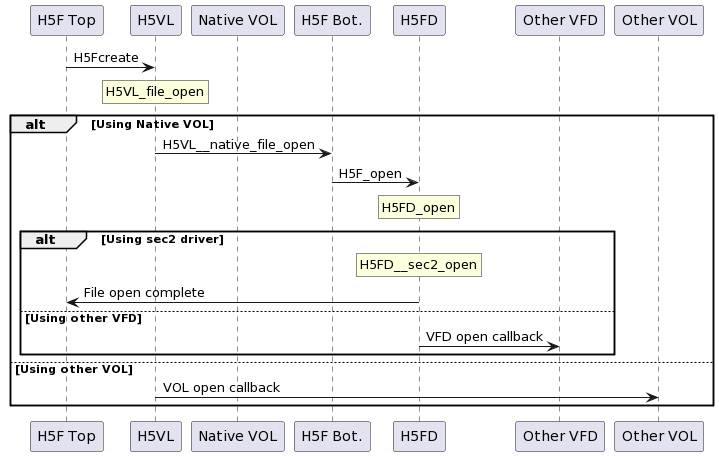
\includegraphics[width=0.80\textwidth]{images/tour-2-uml-vol.png}
\label{fig:tour-2-uml-vol}
\caption{File open through VOL and VFL sequence diagram}
\end{figure}

During this tour, we saw the interplay between the API, the Virtual Object Layer, the native VOL connector, and the Virtual File Layer. We saw how and which API calls are ``routed" through the VOL layer, which is perhaps the most important takeaway. We got a glimpse of how HDF5 files are represented in memory. Along the way, we encountered the metadata cache as one of the central architectural elements of the current library implementation. There is one metadata cache instance per HDF5 file, and rather than being directly controlled by API calls, metadata I/O occurs around metadata cache events indirectly triggered by API calls. While improving overall I/O performance, the ``split nature" of the state of a modified open HDF5 file makes it more vulnerable to unexpected application termination.

With extension interfaces such as VOL and VFD, the HDF5 library's extensibility is apparent but may make the simple creation of an HDF5 file appear overly complicated. However, very few applications stop at creating empty HDF5 files, and we saw some of the benefits of this when examining variants of the empty HDF5 file creation prototype.

During the next tour, we will examine how the HDF5 library handles user (meta-)data.

\section{What is the HDF5 library doing to my data?}\label{sec:tour3}

%|  Name  | TODO | ONGOING | DONE |
%|--------|------|---------|------|
%| Dana   | x    |         |      |
%| Gerd   |      |         |  x   |
%| Glenn  |      |         |  x   |
%| Jordan | x    |         |      |
%| Luke   | x    |         |      |
%| Matt   | x    |         |      |
%| Neil   | x    |         |      |
%| Scot   | x    |         |      |

In the section `IV.B. Disk Format: Level 2B - Data Object Data Storage', the HDF5 file format specification states the following regarding the storage of array values (from datasets or attributes):

\begin{quote}
Multi-dimensional array data is stored in C order; in other words, the ``last" dimension changes fastest.

Data whose elements are composed of atomic datatypes are stored in IEEE format unless they are defined explicitly as being stored in a different machine format with the architecture-type information from the datatype header message. This means that each architecture will need to [potentially] byte-swap data values into the internal representation for that particular machine.

Data with a variable-length datatype is stored in the global heap of the HDF5 file. Global heap identifiers are stored in the data object storage.

Data whose elements are composed of reference datatypes are stored in several different ways depending on the particular reference type involved. Object pointers are just stored as the offset of the object header being pointed to, with the size of the pointer being the same number of bytes as offsets in the file.

Dataset region references are stored as a heap ID, which points to the following information within the file heap: an offset of the object pointed to, number-type information (same format as header message), dimensionality information (same format as header message), sub-set start and end information (in other words, a coordinate location for each), and field start and end names (in other words, a [pointer to the] string indicating the first field included and a [pointer to the] string name for the last field).

Data of a compound datatype is stored as a contiguous stream of the items in the structure, with each item formatted according to its datatype.
\end{quote}

Having read through pages and pages of HDF5 file format intricacies, many readers may find this statement near the end of the document~\cite{ffmt} to sound anticlimactic. Undoubtedly, the writer of these lines must have run out of time or money, and he or she tried to cut corners because this sounds too simple to be true! Well, it is accurate, and the answer to the question, ``What is the HDF5 library doing to my data?" is ``Not much." or ``Not what you might be thinking." Borrowing networking terminology, the HDF5 library is \textit{framing} user data rather than manipulating the data itself. (Here, we ignore specific use cases such as datatype conversion or compression.) Similar to TCP/IP protocol layers (see Figure~\ref{fig:tcpip-protocols}), there are multiple framing layers in the HDF5 file format.

\begin{figure}[h]
    \centering
    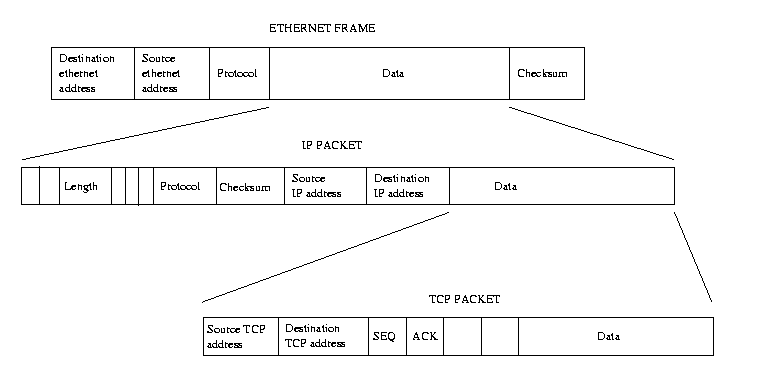
\includegraphics[width=0.75\textwidth]{images/protocols.png}
    \caption{TCP/IP Protocol Layers\cite{tldp2023}}
    \label{fig:tcpip-protocols}
\end{figure}

In this section, we explore how the native VOL performs this ``framing" of user (meta)data. After clarifying the difference between user metadata and user data, we will see why and how it treats them separately. At the end of this tour, the reader should be able to explain Figure~\ref{fig:io-paths} to their colleagues!

\subsection{User metadata and data}

Most applications using HDF5 are there to solve a scientific, engineering, or business problem. Users of the application think in terms of the particular application domain, such as particle velocities, sensor readings, or stock prices. Be that as it may, the application's creator has adopted a convention or profile on representing these domain objects using HDF5 data model entities. Like a mathematical model, in the broadest sense, the HDF5 data model is about variables and the relationships between variables. These variables, or datasets, are array variables (their values are multidimensional arrays), and relationships are expressed by arranging them in graph-like structures with labeled edges or links. Furthermore, datasets and arrangements, or groups, can be decorated by ``small'' (in the domain sense) named array variables, so-called attributes. With the ``grammar" of how these arrangements, or (logical) files, can be put together, this is essentially all there is to the HDF5 data model. In this context, we refer to dataset values (arrays!) as \textit{user data}, and everything else is considered \textit{user metadata}. In other words, user data is the ``heavy-weight" or problem-scale data, proportional to the number of degrees of freedom, the resolution, the spatio-temporal extent, etc. On the other hand, user metadata describes user data, e.g., the unit of the underlying variable, the calibration or sampling rate of an instrument, the time step, etc. Note that dataset metadata, such as rank, extent, element type, etc., is also metadata.

\begin{listing}
\centering
\caption{Dataset life cycle.}
\label{lst:dataset-life-cycle}
\begin{minted}[linenos]{C}
#include "common.h"
int main() {
    hid_t file_id = H5Fcreate("data.h5", H5F_ACC_TRUNC, H5P_DEFAULTx2);
    hid_t fspace = H5Screate_simple(1, (hsize_t[]){10}, NULL);
    hid_t dset = H5Dcreate(file_id, "data", H5T_NATIVE_INT, fspace,
        H5P_DEFAULTx3);
    H5Dclose(dset);
    H5Sclose(fspace);
    H5Fclose(file_id);
    return 0;
}
\end{minted}
\end{listing}

For example, the HDF5 data model instance created by the program in Listing~\ref{lst:dataset-life-cycle} would consist of the array \texttt{[0,0,0,0,0,0,0,0,0,0]} as its user data and metadata such as
\begin{itemize}
    \item The HDF5 file contains a single array variable linked as \texttt{data} in the root group.
    \item The element type of the array variable is ``integers between -2,147,483,648 and 2,147,483,647."
    \item The rank of the array variable is one, and its extent is ten elements.
\end{itemize}
The HDF5 library lets us persist this information in a file system's physical file \texttt{data.h5}.
In Figure~\ref{fig:io-paths}, we show the major library components involved in the framing of this information and suggest that user metadata and data are treated differently.

Following the Callgrind profile of Listing~\ref{lst:dataset-life-cycle}, a call sequence for \texttt{H5Dcreate()} similar to the one shown in Figure~\ref{fig:tour-3-uml-dset-create-contig} emerges. Notice that we have skipped the VOL layer incantation, which applies to \texttt{H5Dcreate()}, and we have suppressed a few details about object header composition and metadata cache entry pinning, etc. The gist of the call sequence is this:

\begin{enumerate}
    \item As a ``side-effect" of linking the newly minted dataset to the root group, we create a dataset object header conforming to the file format specification~\cite{ffmt}.
    \item The object header is placed into the file's metadata cache, and the corresponding entry is marked as dirty. That way, it will get flushed/written to the file when the metadata cache is destroyed (\texttt{H5AC\_dest()}), which happens in the wake of \texttt{H5Fclose()}.
    \item Finally, the freshly minted dataset's file address and link name are added to the root group's symbol table, and the B-tree index is updated.
\end{enumerate}

This sequence covers the left portion of Figure~\ref{fig:io-paths}. What happened to the array? If you follow the Callgrind profile closely, you will notice that no array ever gets created and written. For one, there is no statically or dynamically allocated array in Listing~\ref{lst:dataset-life-cycle}. However, the actual reason is the default behavior of the library that prescribes so-called late allocation for datasets with contiguous layouts. Space allocation in the file is delayed until an element of the dataset is modified, which triggers the allocation and initialization with fill values for elements that aren't modified. In other words, nothing happens in the right portion of Figure~\ref{fig:io-paths} for this simple example. It's a pure metadata affair.

\begin{comment}
http://www.plantuml.com/plantuml/
@startuml
participant "H5D top" as t_h5d
participant "H5D bot." as b_h5d
participant H5L
participant H5G
participant H5O
participant H5AC
participant H5B

t_h5d -> b_h5d: H5D__create_named
b_h5d -> H5L: H5L_link_object
H5L -> H5G: H5G_traverse
H5G -> H5O: H5O_obj_create
H5O -> b_h5d: H5D__create
b_h5d -> H5O: H5O_create
rnote over H5O: H5O_create_ohdr
rnote over H5O: H5O_apply_ohdr
H5O -> H5AC: H5AC_insert_entry
H5O -> H5AC: H5AC_mark_entry_entry
H5L -> H5G: H5G_obj_insert
H5G -> H5O: H5O_link
rnote over H5G: H5G_stab_insert
H5G -> H5B: H5B_insert
H5B -> H5G: H5G__node_insert
@enduml
\end{comment}

\begin{figure}
    \centering
    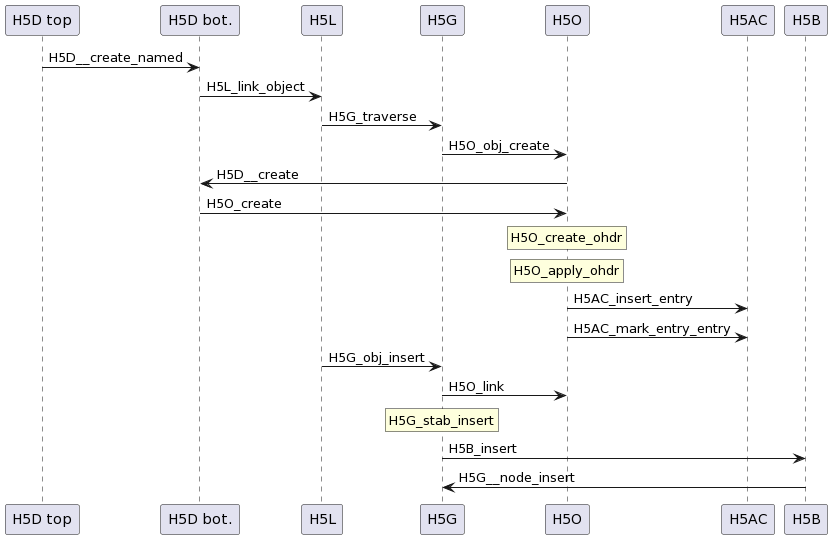
\includegraphics[width=0.80\textwidth]{images/tour_3_uml_dset_create.png}
    \caption{Process to create a contiguous dataset.}
    \label{fig:tour-3-uml-dset-create-contig}
\end{figure}

The dataflow for datasets is similar to files in that the in-memory representation has top (\texttt{H5D\_t}) and bottom (\texttt{H5D\_shared\_t}) portions. Both are defined in \texttt{H5Dpkg.h}. The top portion is unique to each instance of an opened dataset, and the bottom portion is a shared struct that is only created once for a given dataset. (The dataset's object header is constructed from the information in the bottom portion.) Thus, if a dataset is opened twice, there will be two handles (IDs) and two \texttt{H5D\_t} structs, both sharing one \texttt{H5D\_shared\_t}.

\subsection{Data transfer}\label{sec:data-transfer}

To activate the right portion of Figure~\ref{fig:io-paths}, we call \texttt{H5Dwrite()}, as shown in Listing~\ref{lst:dataset-transfer}. The key elements of the user data journey are captured in Figure~\ref{fig:tour-3-uml-dset-write-contig}. We can see that storage for the data is allocated in the file. There is, however, a twist: the data is not written into the file when \texttt{H5Dwrite()} is called or completed. Because the array to be written is so small, the data is copied to a buffer, and the write is delayed until the dataset is closed, when it is flushed (\texttt{H5D\_\_flush\_sieve\_buf()}). The native VOL uses a so-called data sieve buffer to reduce the number of small I/O operations. (We will have more to say about the sieve buffer in section~\ref{sec:tour6}.)

\begin{listing}
\centering
\caption{Data transfer.}
\label{lst:dataset-transfer}
\begin{minted}[linenos]{C}
#include "common.h"
int main() {
    hid_t file_id = H5Fcreate("data.1.h5", H5F_ACC_TRUNC, H5P_DEFAULTx2);
    hid_t fspace = H5Screate_simple(1, (hsize_t[]){10}, NULL);
    hid_t dset = H5Dcreate(file_id, "data", H5T_NATIVE_INT, fspace,
        H5P_DEFAULTx3);
    int data[10] = {0,1,2,3,4,5,6,7,8,9};
    H5Dwrite(dset, H5T_NATIVE_INT, H5S_ALL, H5S_ALL, H5P_DEFAULT, data);
    H5Dclose(dset);
    H5Sclose(fspace);
    H5Fclose(file_id);
    return 0;
}
\end{minted}
\end{listing}

\begin{comment}
http://www.plantuml.com/plantuml/
@startuml
participant "H5D top" as t_h5d
participant "H5D bot." as b_h5d
participant H5FL
participant H5FD

t_h5d -> b_h5d: H5VL__native_dataset_write
rnote over b_h5d: H5D__write
rnote over b_h5d: H5D__ioinfo_init
rnote over b_h5d: H5D__alloc_storage
rnote over b_h5d: H5D__contig_write
rnote over b_h5d: H5D__select_io
rnote over b_h5d: H5D__contig_writevv
rnote over b_h5d: H5D__contig_writevv_sieve_cb
b_h5d -> H5FL: H5FL_blk_calloc
t_h5d -> b_h5d: H5VL__native_dataset_close
rnote over b_h5d: H5D_close
rnote over b_h5d: H5D__contig_flush
rnote over b_h5d: H5D__flush_sieve_buf

b_h5d -> H5FD: H5FD_write
rnote over H5FD: H5FD__sec2_write
@enduml
\end{comment}

\begin{figure}
    \centering
    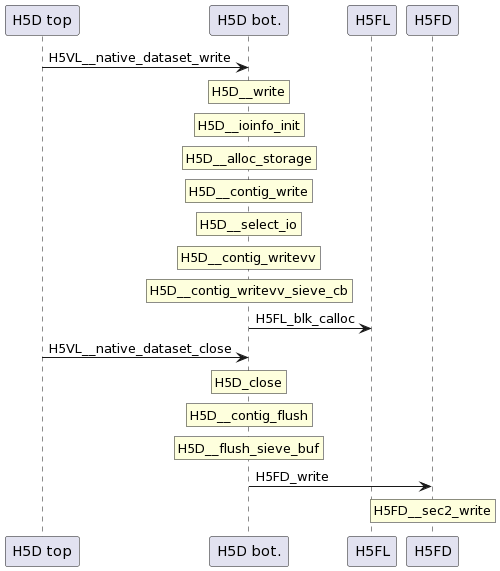
\includegraphics[width=0.55\textwidth]{images/tour_3_uml_dset_write.png}
    \caption{Process to write a (small) contiguous dataset.}
    \label{fig:tour-3-uml-dset-write-contig}
\end{figure}


\subsection{Chunked storage layouts, selections \& partial I/O}\label{sec:layouts-selections}

The flow discussed in section~\ref{sec:data-transfer} places us in the right portion of Figure~\ref{fig:io-paths}. However, we haven't exercised much of the machinery shown there. To activate a few of those components, we modify the storage layout and write only parts of the dataset, as shown in Listing~\ref{lst:dataset-chunky}.

\begin{listing}
\centering
\caption{Data -- chunked layout, selection, \& partial I/O.}
\label{lst:dataset-chunky}
\begin{minted}[linenos]{C}
#include "common.h"
int main() {
    hid_t file = H5Fcreate("data.3.1.h5", H5F_ACC_TRUNC, H5P_DEFAULTx2);
    hid_t fspace = H5Screate_simple(1, (hsize_t[]){10}, NULL);
    hid_t dcpl = H5Pcreate(H5P_DATASET_CREATE);
    H5Pset_chunk(dcpl, 1, (hsize_t[]){6});
    hid_t dset = H5Dcreate(file, "data", H5T_NATIVE_INT, fspace,
        H5P_DEFAULT, dcpl, H5P_DEFAULT);
    int data[5] = {1,3,5,7,9};
    hid_t mspace = H5Screate_simple(1, (hsize_t[]){5}, NULL);
    H5Sselect_all(mspace);
    H5Sselect_hyperslab(fspace, H5S_SELECT_SET, (hsize_t[]){1}, (hsize_t[]){2},
        (hsize_t[]){5}, (hsize_t[]){1});
    H5Dwrite(dset, H5T_NATIVE_INT, mspace, fspace, H5P_DEFAULT, data);
    H5Dclose(dset);
    H5Sclose(mspace);
    H5Pclose(dcpl);
    H5Sclose(fspace);
    H5Fclose(file);
    return 0;
}
\end{minted}
\end{listing}

The changes compared to the sequence shown in Figure~\ref{fig:tour-3-uml-dset-write-contig} are shown in Figure~\ref{fig:tour-3-uml-dset-write-chunk}.

\begin{comment}
http://www.plantuml.com/plantuml/
@startuml
participant "H5D top" as t_h5d
participant "H5D bot." as b_h5d
participant H5B
participant H5S
participant H5F

hnote over b_h5d #FFAAAA: Change in storage allocation

rnote over b_h5d: H5D__create
rnote over b_h5d: H5D__update_oh_info
rnote over b_h5d: H5D__layout_oh_create
rnote over b_h5d: H5D__chunk_init
rnote over b_h5d: H5D__btree_idx_init
b_h5d -> H5B: H5B_shared_new

hnote over H5S #FFAAAA: Selection construction

rnote over H5S: H5S_select_hyperslab
rnote over H5S: H5S__hyper_regular_and_single_block
rnote over H5S: H5S__generate_hyper_slab
rnote over H5S: H5S__make_hyper_spans

hnote over b_h5d #FFAAAA: Change in write path

t_h5d -> b_h5d: H5VL__native_dataset_write
rnote over b_h5d: H5D__write
rnote over b_h5d: H5D__chunk_io_init
rnote over b_h5d: H5D__alloc_storage
rnote over b_h5d: H5D__chunk_create
rnote over b_h5d: H5D__chunk_write
rnote over b_h5d: H5D__select_write
rnote over b_h5d: H5D__select_iter_init

hnote over b_h5d #FFAAAA: Change in dataset close
t_h5d -> b_h5d: H5VL__native_dataset_close
rnote over b_h5d: H5D_close
rnote over b_h5d: H5D__chunk_flush
rnote over b_h5d: H5D__chunk_file_alloc
b_h5d -> H5F: H5F_shared_block_write
rnote over b_h5d: H5D__btree_idx_insert
rnote over b_h5d: H5D__chunk_cinfo_cache_update
@enduml
\end{comment}

\begin{figure}
    \centering
    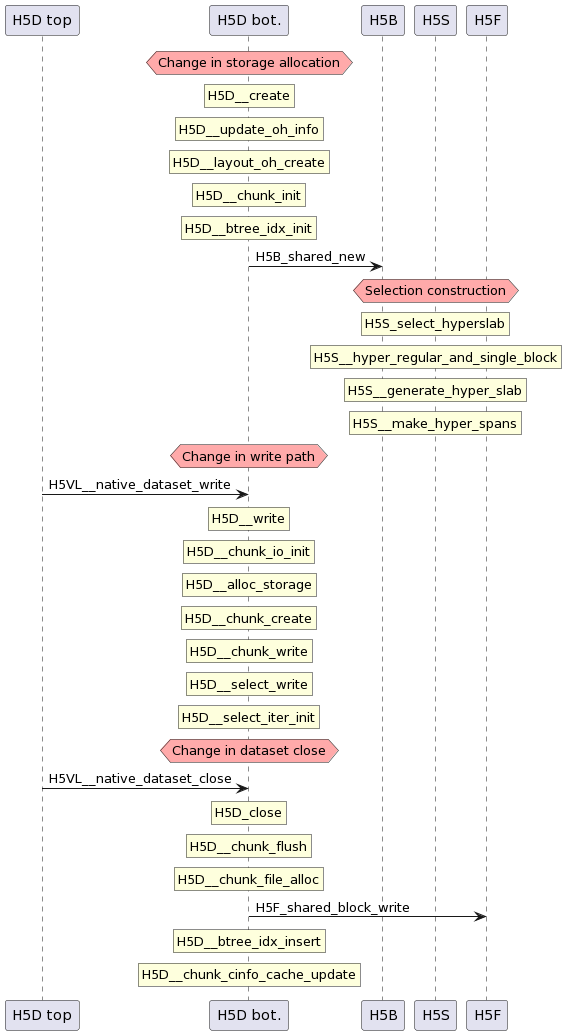
\includegraphics[width=0.55\textwidth]{images/tour_3_uml_dset_write_sel.png}
    \caption{Process to write a selection to a (small) chunked dataset.}
    \label{fig:tour-3-uml-dset-write-chunk}
\end{figure}

The gist is this:
\begin{enumerate}
    \item The different storage layout (chunked) is noted in the dataset's object header at creation time. The chunk locations are tracked with a B-tree index. Not that, as in the contiguous case, chunk allocation is delayed until any actual data is written.
    \item The hyperslab selection construction is a 100\% in-memory metadata affair and is \textit{not} routed through the VOL interface.
    \item The function \texttt{H5Dwrite()} is responsible for allocating chunks and iterating through selections. However, data is not written immediately if the array and chunk sizes are small. Instead, it is written only after the dataset is closed and flushed. The actual writing of user data is done by \texttt{H5F\_shared\_block\_write()}. After writing, the chunk index is updated.
\end{enumerate}

While we have not yet explored the native VOLs facilities for datatype conversion, data filtering, or data caching and buffering, we have seen enough to corroborate the claim that the native VOL does not alter user data. Instead, it frames the data and augments them with metadata to create a self-describing package called a native HDF5 file. In section~\ref{sec:user-metadata}, we explore how an everyday kind of user-metadata, attributes, fares under the scheme outlined in Figure~\ref{fig:io-paths}.

\subsection{User-defined metadata -- The life cycle of an HDF5 attribute}\label{sec:user-metadata}

\paragraph{Overview} Attributes' purpose is to associate metadata with HDF5 objects directly. Attributes have a very similar interface to datasets - they have a layout defined by a dataspace, contain user data with a datatype determined at creation, and can be written to and read from. Attribute operations pass through the Virtual Object Layer to reach the active VOL connector's storage implementation.

Because attributes exist primarily as metadata, they are distinct from datasets in a few key ways. Attributes are always associated with a parent object: a dataset, group, or committed datatype. Attributes can only be accessed through their parent object, and attribute names are significant only within that parent object. Because they exist entirely as metadata in storage by default, attributes should generally contain less than 64KiB of data (see the "Attribute storage layouts" section for handling larger attributes). For the same reason, an attribute's data must be read or written entirely in every access; partial reading or writing using a selection is not allowed.

\begin{listing}
\centering
\caption{Attribute life cycle.}
\label{lst:attribute-life-cycle}
\begin{minted}[linenos]{C}
#include "common.h"
int main() {
  hid_t file_id = H5Fcreate("attrib.1.h5", H5F_ACC_TRUNC, H5P_DEFAULTx2);
  hid_t scalar = H5Screate(H5S_SCALAR);
  hid_t attr_id =
      H5Acreate(file_id, "meta", H5T_NATIVE_INT, scalar, H5P_DEFAULTx2);
  int meta = 42;
  H5Awrite(attr_id, H5T_NATIVE_INT, &meta);
  H5Aclose(attr_id);
  H5Sclose(scalar);
  H5Fclose(file_id);
  return 0;
}
\end{minted}
\end{listing}

\paragraph{Attributes as objects} Listing~\ref{lst:attribute-life-cycle} shows the life cycle of an attribute. It is created on a parent object, in this case (the root group of) the file \texttt{attrib.1.h5}. It is created with a dataspace and datatype defining the data it stores. Data is written to the attribute in storage, and then the in-memory object for the attribute is closed. 

\begin{listing}
\centering
\caption{Dense storage used with many attributes}
\label{lst:attribute-dense-storage-many}
\begin{minted}[linenos]{C}
#include "common.h"
int main() {
  hid_t fapl_id = H5Pcreate(H5P_FILE_ACCESS);
  hid_t fcpl_id = H5Pcreate(H5P_FILE_CREATE);
  H5Pset_libver_bounds(fapl_id, H5F_LIBVER_V18, H5F_LIBVER_LATEST);
  /* Max in compact storage = 2, min in dense storage = 2 */
  H5Pset_attr_phase_change(fcpl_id, 2, 2);
  hid_t file_id = 
    H5Fcreate("attrib.2.h5", H5F_ACC_TRUNC, H5P_DEFAULT, fapl_id);
  hid_t scalar = H5Screate(H5S_SCALAR);
  hid_t attr_id1 =
      H5Acreate(file_id, "attr1", H5T_NATIVE_INT, scalar, H5P_DEFAULTx2);
  hid_t attr_id2 =
      H5Acreate(file_id, "attr2", H5T_NATIVE_INT, scalar, H5P_DEFAULTx2);
  /* More than 2 compact attributes - all are moved to dense */
  hid_t attr_id3 =
      H5Acreate(file_id, "attr3", H5T_NATIVE_INT, scalar, H5P_DEFAULTx2);
  H5Aclose(attr_id1);
  H5Aclose(attr_id2);
  H5Aclose(attr_id3);
  H5Adelete(file_id, "attr2");
  H5Adelete(file_id, "attr3");
  /* Less than 2 dense attributes - the rest are moved to compact */
  H5Sclose(scalar);
  H5Fclose(file_id);
  H5Pclose(fapl_id);
  H5Pclose(fcpl_id);
  return 0;
}
\end{minted}
\end{listing}

When an attribute is opened, the library handle points to an instance of \texttt{H5A\_t}. The shared attribute information attached to this structure contains pointers to the attribute's datatype and dataspace, as well as its creation index on its parent object if creation index tracking was enabled at object creation time. Because the creation index is only computed when the attribute is first created or opened, operations such as removing attributes could cause it to become invalid (e.g. its creation index could exceed the total number of attributes on the parent object). This is why, before an attribute is deleted from its parent object, identifiers of other attributes on that object should be closed, and only re-opened after the attribute deletion is complete.

\begin{listing}
\centering
\caption{Dense storage used with a large attribute}
\label{lst:attribute-dense-storage-large}
\begin{minted}[linenos]{C}
#include "common.h"
int main() {
  hid_t fapl_id = H5Pcreate(H5P_FILE_ACCESS);
  H5Pset_libver_bounds(fapl_id, H5F_LIBVER_V18, H5F_LIBVER_LATEST);
  hid_t file_id = 
    H5Fcreate("attrib.3.h5", H5F_ACC_TRUNC, H5P_DEFAULT, fapl_id);
  hid_t scalar = H5Screate(H5S_SCALAR);
  /* One element is 4*2*512*512 = ~4194K bytes (with 4-byte integers)
   * Will automatically be put into dense storage */
  hid_t dtype = H5Tarray_create(H5T_NATIVE_INT, 2, (hsize_t[]){512, 512});
  hid_t attr_id = H5Acreate(file_id, "image", dtype, scalar, H5P_DEFAULTx2);
  int meta[512][512];
  H5Awrite(attr_id, dtype, &meta);
  H5Aclose(attr_id);
  H5Tclose(dtype);
  H5Sclose(scalar);
  H5Fclose(file_id);
  H5Pclose(fapl_id);
  return 0;
}
\end{minted}
\end{listing}


\subsection{Attribute storage layouts} 

\paragraph{Overview} There are two primary ways that attributes may be stored - 'compact' storage and 'dense' storage. Compact attributes are small and few in number, and are stored in the header of their parent object. Dense attributes are large or many in number, and are stored in the file's global fractal heap. There is a technique that could be considered a third metadata storage method: Using attributes with reference datatypes to point at metadata stored in other objects. 

\paragraph{Compact Storage} When attributes are in compact storage, they are stored as attribute messages in the object header of their parent object. An attribute is stored compactly if it is below 64KiB in size and the parent object's total number of attributes is below its max compact storage threshold defined by \texttt{H5Pset\_attr\_phase\_change()}.

Figure~\ref{fig:tour-3-uml-attr-create-compact} is a diagram of the library's internal process to create an attribute in compact storage with the native VOL connector. First, \texttt{H5O\_\_attr\_create()} uses \texttt{H5O\_pin()} to 'pin' the object header, preventing it from being flushed from the cache to storage until it is unpinned at the end of the operation. Once it is determined that the new attribute should be compact, \texttt{H5O\_\_msg\_append\_real()} handles creating the new attribute message and inserting it into the object header. This is done in two steps: First, \texttt{H5O\_\_msg\_alloc()} creates a new message in the header, and returns its location within the header. Then, \texttt{H5O\_\_copy\_mesg()} uses the copy callback of the message type to populate the newly created message. In this case, the new message is an attribute message providing the copy callback \texttt{H5O\_\_attr\_copy()}, a wrapper around the library's function for copying attributes, \texttt{H5A\_\_copy()}. The generic attribute copy function may be used here because attribute messages contain copies of the native \texttt{H5A\_t} object.

\begin{comment}
http://www.plantuml.com/plantuml/
@startuml
participant H5A
participant H5O

H5A -> H5O: H5A__create
rnote over H5O: H5O__attr_create()

hnote over H5O #FFAAAA: Object header is pinned

rnote over H5O: H5O__msg_append_real
rnote over H5O: H5O__msg_alloc
rnote over H5O: H5O__copy_mesg
H5O -> H5A: H5O__attr_copy
rnote over H5A: H5A__copy

hnote over H5O #FFAAAA: Object header is unpinned
@enduml
\end{comment}

\begin{figure}
    \centering
    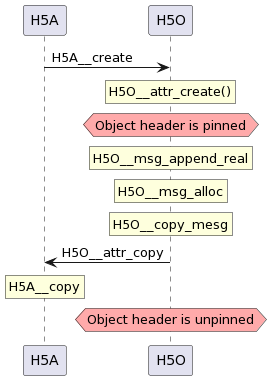
\includegraphics[width=0.30\textwidth]{images/tour_3_uml_attr_create_compact.png}
    \caption{Process to create a compact attribute}
    \label{fig:tour-3-uml-attr-create-compact}
\end{figure}

Figure~\ref{fig:tour-3-uml-attr-remove-compact} is a diagram of the library's internal process to remove a compact attribute. Once again, the object header is pinned to prevent it from being flushed during an operation. The attribute messages in the object header are iterated over in \texttt{H5O\_\_mesg\_iterate\_real()}, and the callback \texttt{H5O\_\_attr\_remove\_cb()} is executed on each. If the attribute message matches the name of the attribute to be deleted, then the deletion process is performed by \texttt{H5O\_\_release\_mesg()}. The removal of the object header message takes place in two parts: first, \texttt{H5O\_\_delete\_msg()} is used to invoke the attribute message's delete callback, \texttt{H5O\_\_attr\_delete()}, which deletes header messages that were referred to by this attribute - specifically, dataspace and datatype messages. After that, \texttt{H5O\_\_msg\_free\_mesg()} invokes the attribute message's 'free' callback, to free the native information stored in the attribute message - the \texttt{H5A\_t} structure and its associated memory.

\begin{comment}
http://www.plantuml.com/plantuml/
@startuml
participant H5A
participant H5O

rnote over H5A: H5Adelete
H5A -> H5O: (...)           
rnote over H5O: H5O__attr_remove

hnote over H5O #FFAAAA: Object header is pinned
rnote over H5O: H5O__msg_iterate_real
H5O -> H5O: Attr msg found
rnote over H5O: H5O__attr_remove_cb
rnote over H5O: H5O__release_mesg
rnote over H5O: H5O__delete_mesg
H5O -> H5O: H5O__attr_delete

H5O -> H5A: H5O__msg_free_mesg
rnote over H5A: H5A__close

hnote over H5O #FFAAAA: Object header is unpinned
@enduml
\end{comment}

\begin{figure}
    \centering
    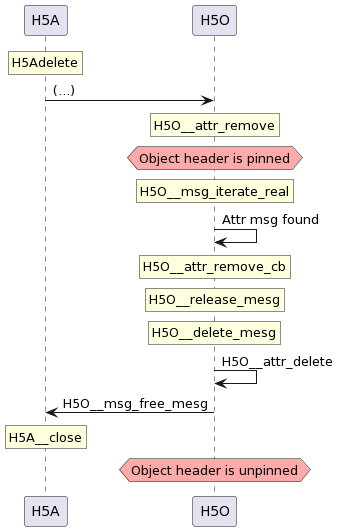
\includegraphics[width=0.35\textwidth]{images/tour_3_uml_attr_remove_compact.png}
    \caption{Removal of a compact attribute}
    \label{fig:tour-3-uml-attr-remove-compact}
\end{figure}

Compact attributes have some drawbacks - performance suffers when objects have many compact attributes and they are strictly limited in size to fit within the object header.  Both of these limitations are circumvented by dense storage. 

\paragraph{Dense Storage} When an attribute is in dense storage, the object header contains a pointer to the location of the attribute's data on disk rather than containing the attribute's data directly.

\begin{comment}
http://www.plantuml.com/plantuml
@startuml
participant H5A
participant H5O
participant H5HF
participant H5B2

H5A -> H5O: H5A__create
rnote over H5O: H5O__attr_create()
hnote over H5O #FFAAAA: Object header is pinned
H5O -> H5A:

opt Fractal heap does not yet exist
rnote over H5A: H5A__dense_create
H5A -> H5HF: Create fractal heap in the file
rnote over H5HF: H5HF_create
H5A -> H5B2: Create name index B-tree
rnote over H5B2: H5B2_create

opt If ceation order is tracked
H5A -> H5B2: Create creation order B-tree
rnote over H5B2: H5B2_create
end
end

rnote over H5A: H5A__dense_insert

alt If attribute message is shared 
rnote over H5A: Copy pre-existing heap ID
else Attribute message is not shared

H5A -> H5HF: Insert attr into fractal heap
rnote over H5HF: H5HF_insert
end

H5A -> H5B2: Insert attr name into name B-tree
rnote over H5B2: H5B2_insert

opt If creation order is tracked
H5A -> H5B2: Insert record into creation order B-tree
rnote over H5B2: H5B2_insert
end

hnote over H5O #FFAAAA: Object header is unpinned
@enduml
\end{comment}

\begin{figure}
    \centering
    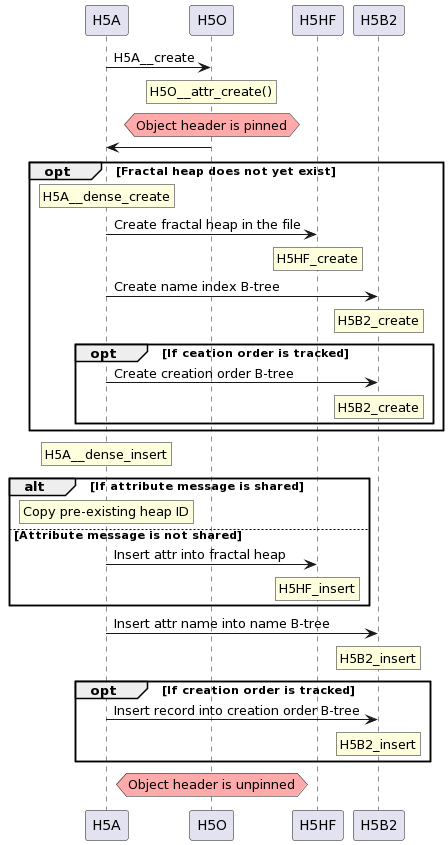
\includegraphics[width=0.5\textwidth]{images/tour_3_uml_attr_create_dense.png}
    \caption{Attribute insertion into dense storage}
    \label{fig:tour-3-uml-attr-create-dense}
\end{figure}

\begin{comment}
http://www.plantuml.com/plantuml
@startuml
participant H5A
participant H5O

rnote over H5A: H5Adelete
H5A -> H5O: (...)
rnote over H5O: H5O__attr_remove

hnote over H5O #FFAAAA: Object header is pinned
H5O -> H5A:
rnote over H5A: H5A__dense_remove
H5A -> H5B2: Remove from name index B-tree
rnote over H5B2: H5B2_remove

opt Creation order is tracked
H5A -> H5B2: Remove from creation order B-tree
rnote over H5B2: H5B2_remove
end

alt If attribute is shared
H5A -> H5SM:
rnote over H5SM: H5SM_delete

else If attribute is not shared 
H5A -> H5O: Delete dtype/dataspace
rnote over H5O: H5O__attr_delete
H5A -> H5HF:
rnote over H5HF: H5HF_remove 
end 

hnote over H5O #FFAAAA: Object header is unpinned
@enduml
\end{comment}

\begin{figure}
    \centering
    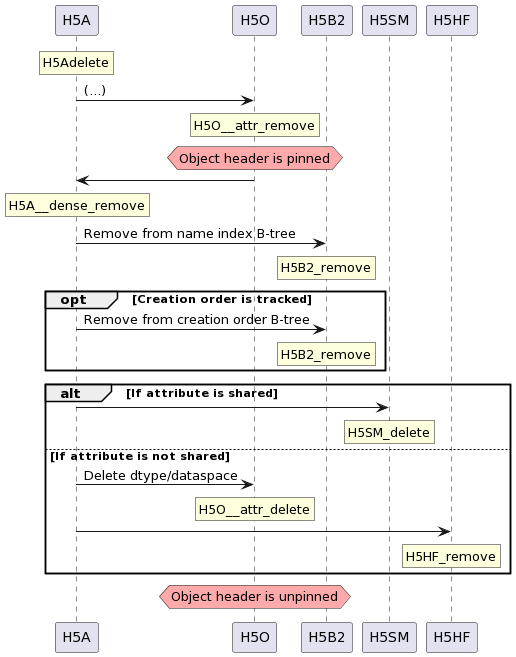
\includegraphics[width=0.65\textwidth]{images/tour_3_uml_attr_remove_dense}
    \caption{Attribute deletion in dense storage}
    \label{fig:tour-3-uml-attr-remove-dense}
\end{figure}

There are two circumstances under which a new attribute is placed into dense storage. The first is that the number of attributes on the parent object exceeds the maximum number of compact attributes on the object. This threshold may be specified for each object using \texttt{H5P\_set\_attr\_phase\_change()}. The second is that the size of the attribute exceeds 64k bytes, and it would not fit into compact storage. All pre-existing attributes are moved to dense storage whenever a new attribute is placed into dense storage. 

Figure~\ref{fig:tour-3-uml-attr-create-dense} shows the library's internal process to create an attribute in dense storage. The object header is still pinned, even though the new attribute is not to be stored in the object header. This is because the attribute creation may have side effects that require modifying the object header. If this file does not yet have a fractal heap for dense attribute storage, one is created with \texttt{H5A\_\_dense\_create()}. This step also involves the creation of a B-tree to map dense attribute names to attribute information and optionally creating a B-tree to make the attribute information available by creation order. Once the dense attribute storage structures are confirmed, the attribute's information is stored densely by \texttt{H5A\_\_dense\_insert()}. This involves using the attribute message's encode callback to serialize the attribute, and this serialized attribute information is inserted into the fractal heap by \texttt{H5HF\_insert()}. If the attribute is shared, then this attribute points to the information of an attribute that already exists in the fractal heap. In this case, the insertion into the fractal heap is skipped, and the heap ID of the existing attribute in the fractal heap is copied. The heap information of the new attribute (or preexisting shared attribute) is stored in the name-index B-tree, to be accessed later by the hash of the attribute name. Lastly, if the creation order is tracked, the heap information is also inserted into the creation-order B-tree, to be accessed later by link creation order.

Figure~\ref{fig:tour-3-uml-attr-remove-dense} shows the library's internal process to remove an attribute from dense storage. After \func{H5O__attr_remove} determines the target attribute is in dense storage, \func{H5A__dense_remove} performs the removal. \func{H5B2_remove} searches the name-index B-tree and removes the information for the dense link. If creation order is tracked, the same operation is performed on the creation order B-tree. If the dense attribute is shared between objects, the 'deletion' is handled by using \func{H5SM_delete} to decrease the reference count of the shared attribute message. Otherwise, the dense attribute's referenced information (dataspace/datatype messages) is deleted by \func{H5O__attr_delete}, and it is removed from the dense attribute fractal heap.

When an attribute is removed from storage, the remaining attributes may be moved back into compact storage. If two conditions are met, an attribute will be moved back to compact storage. First, the total number of remaining attributes must be below the minimum number of dense attributes on the object, another threshold set by \texttt{H5P\_set\_attr\_phase\_change()}. Second, the attribute must be under 64k bytes in size. It is possible for the removal of an attribute to cause some, but not all, of the remaining attributes to be moved to compact storage due to some being too large to store compactly. 

\paragraph{Attribute Storage and File Format Versions}  Note that because it affects how the HDF5 file is stored on disk, using dense attribute storage requires allowing the library to use a 1.8+ version of the file format (i.e. using \texttt{H5Pset\_libver\_bounds()} with a low version $\geq$ 1.8). With a pre-1.8 compatible file format version, attribute storage will always be compact, and attempts to create attributes greater than 64KiB in size will fail. Pre-1.8 compatible large metadata storage can be accomplished by storing metadata as datasets.

\subsection{Summary} 

Attributes provide a flexible way to store metadata on an HDF5 object with the same CRUD interface as datasets. By default, attributes are stored compactly in the object header with other object metadata. The library takes advantage of the properties of B-trees and fractal heaps for large attributes or large amounts of attributes. If backward compatibility or compressibility is required for metadata, it may be stored in datasets and accessed from other objects through references.

From the perspective of the native VOL, user metadata and data travel down two different ``swim lanes," as depicted in Figure~\ref{fig:io-paths}. The main reason is their different role and functions in the HDF5 data model, which leads to different operations being supported in efficient and practical implementations.

\begin{landscape}
\begin{sidewaysfigure}[!ht]
%\begin{figure}[h!]
\centering
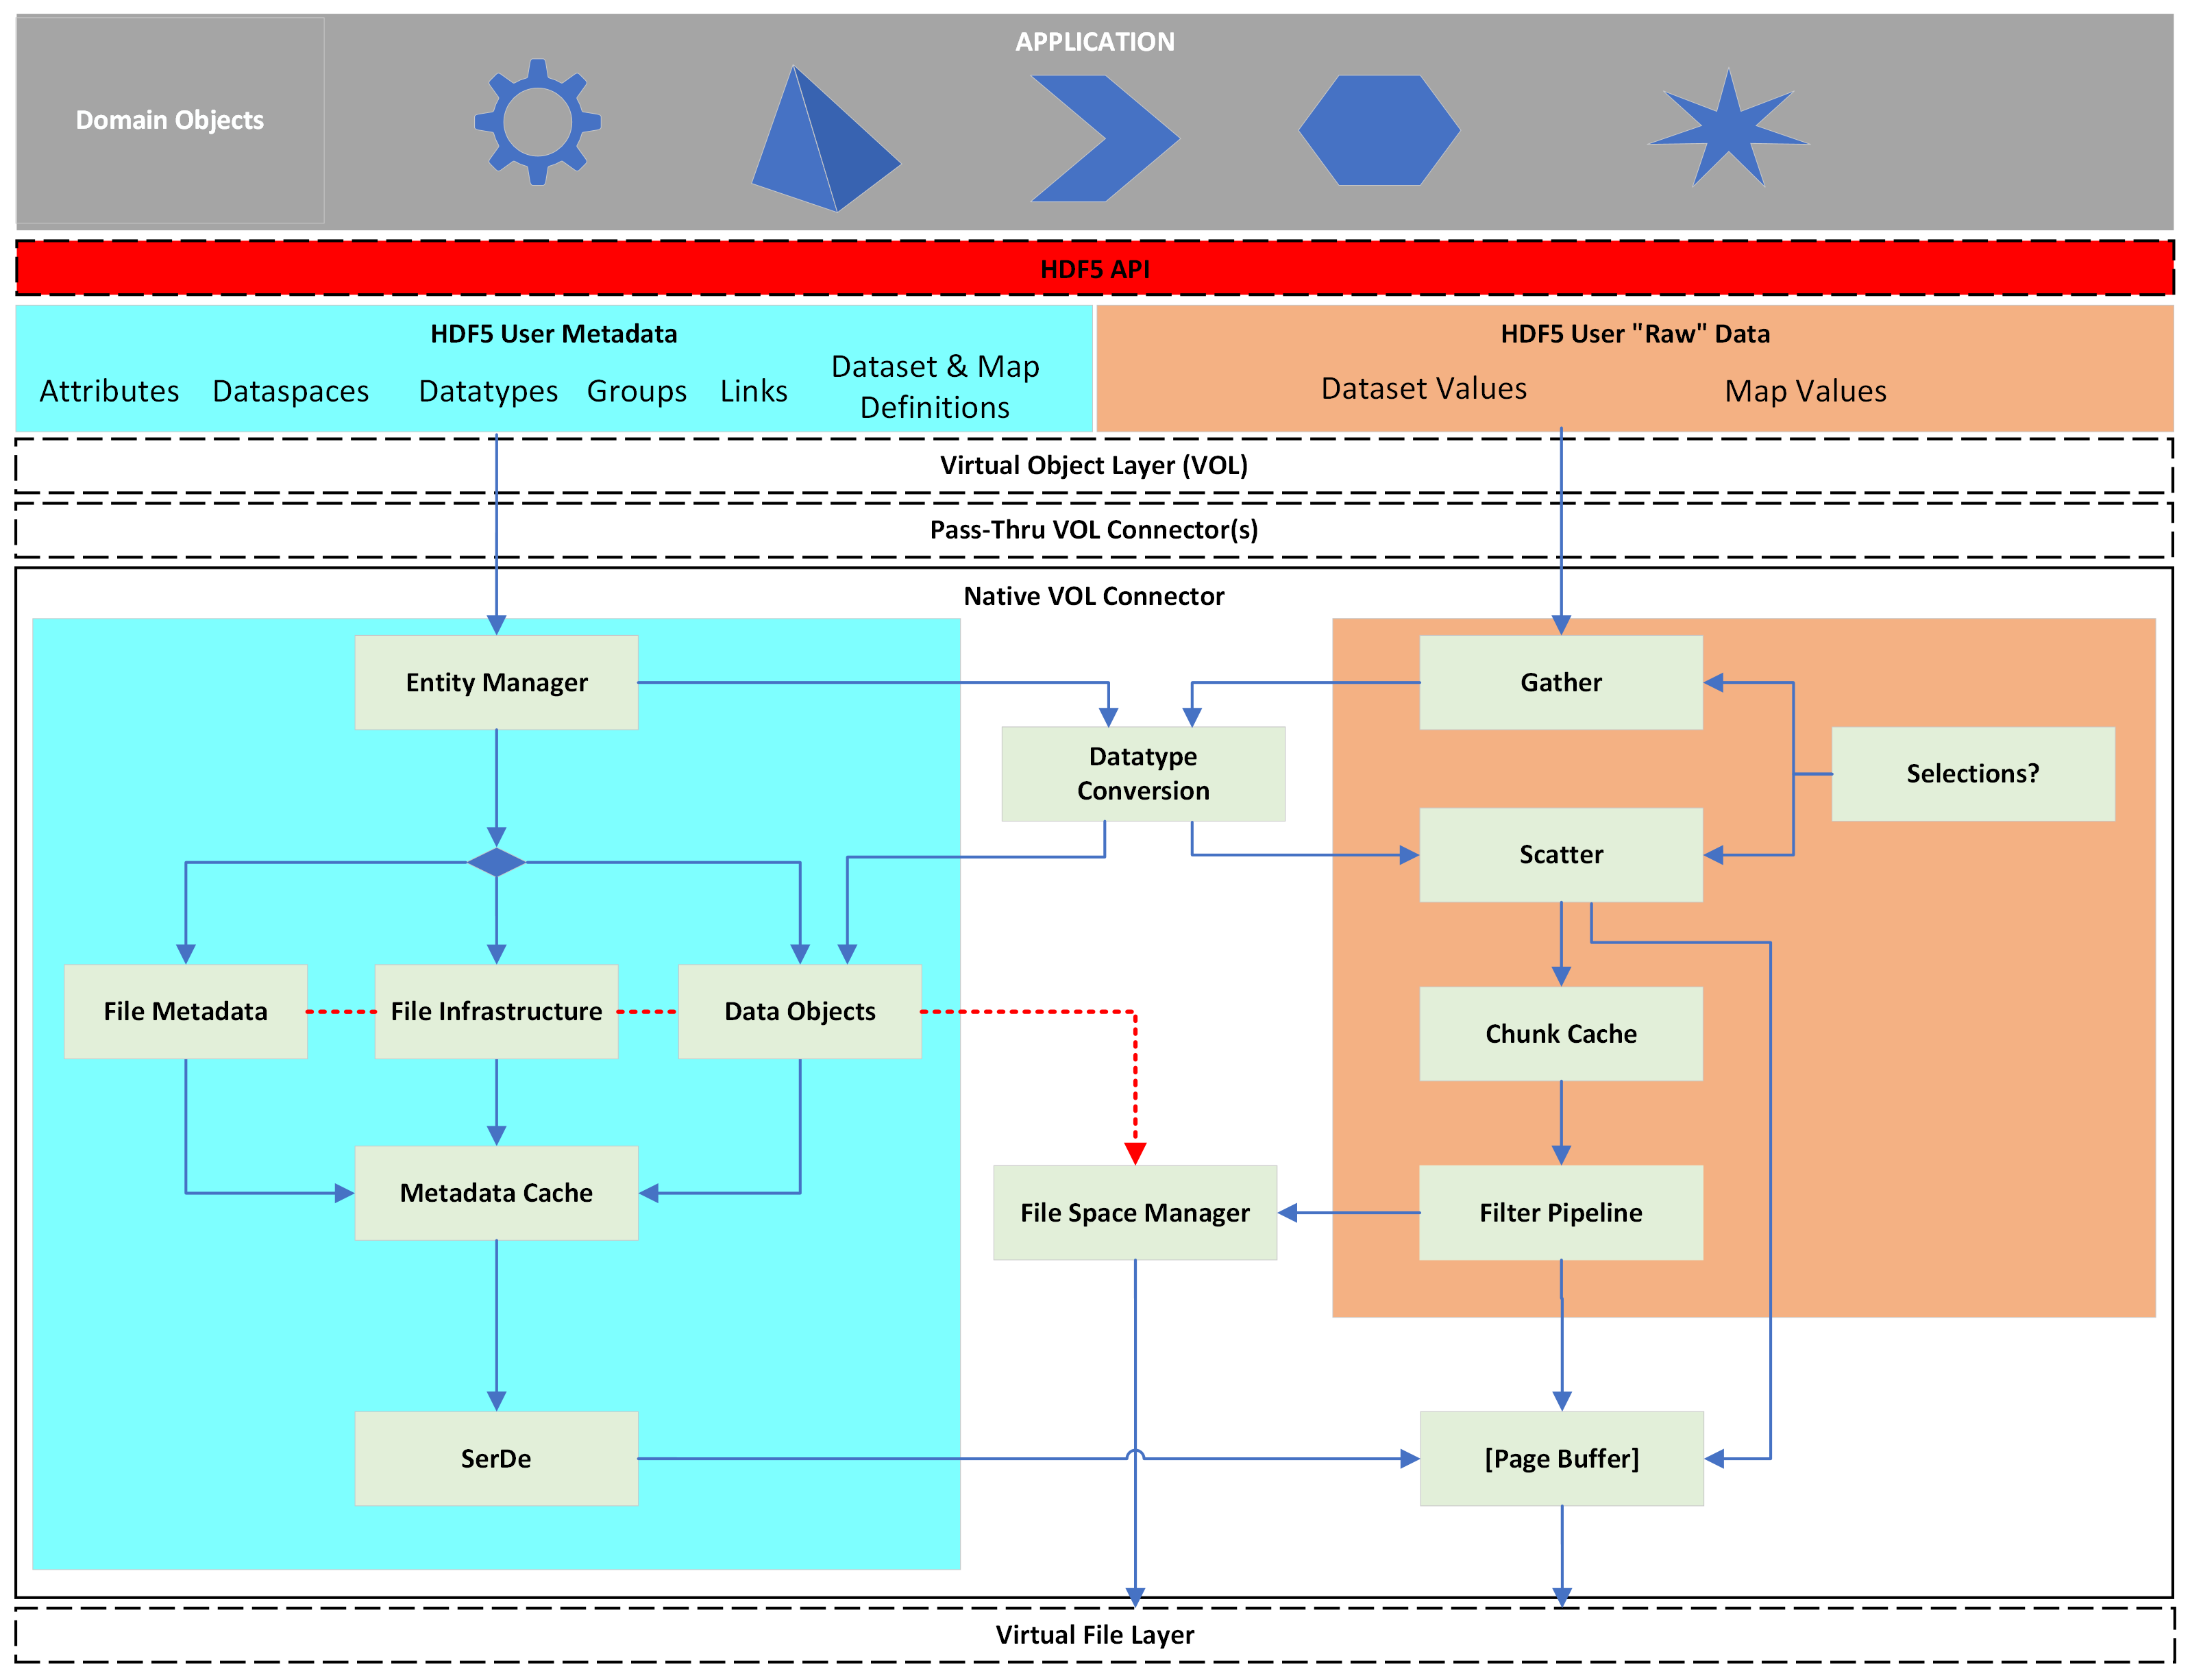
\includegraphics[scale=0.74,angle=90]{images/HDF5 library meta data.png}
\caption{The different I/O paths for metadata and ``raw'' data through the HDF5 library.\label{fig:io-paths}}
%\end{figure}
\end{sidewaysfigure}
\end{landscape}

\section{The H Stands for Hierarchical}\label{chap:groups-and-links}

%|  Name  | TODO | ONGOING | DONE |
%|--------|------|---------|------|
%| Dana   | x    |         |      |
%| Gerd   |      |         |  x   |
%| Glenn  |      |         |  x   |
%| Jordan | x    |         |      |
%| Luke   | x    |         |      |
%| Matt   |      |         |  x   |
%| Neil   | x    |         |      |
%| Scot   | x    |         |      |

A somewhat twisted reading of `Hierarchical Data Format' might create the idea that there might be something hierarchical about the file format. There indeed are a few discernible layers in the file format specification~\cite{ffmt}, and we used the TCP/IP protocol metaphor (see Figure~\ref{fig:tcpip-protocols}) to explain how the native VOL frames user metadata and data into portable self-describing packages, but this would be a rather uninteresting hierarchy, and none that would help users. What's hierarchical about HDF5 is how the object namespace is realized through groups and links, which differs fundamentally from hierarchies that can be mimicked in key-value representations. Not only is the file-system-in-a-file metaphor apt, but an HDF5 file is also a \textit{web-in-a-file}.

\subsection{Groups}

\paragraph{Overview} Groups are a key aspect of an HDF5 file's hierarchical structure. A minimal example of group creation is shown in Listing~\ref{lst:group-life-cycle}.

It is often said that named HDF5 objects (datasets, groups, and committed datatypes) reside in groups. To be more precise, groups contain link objects that point to named HDF5 objects. When a named object is created, a link that points to it is also created. It is this link that is written to the group's object header in storage. This is why \func{H5Dcreate}, \func{H5Tcommit}, and \func{H5Gcreate} all take a link creation property list as an argument.

Figure~\ref{fig:tour-4-uml-group-create} shows the library's internal process to create a new group through the native VOL. The application calls the API function \func{H5Gcreate}, and because groups are (generally) named objects, \func{H5G__create_named} is invoked. After creating a new group in an HDF5 file, \func{H5L_link_object} links it into the HDF5 file hierarchy. This linking process involves creating a link using \func{H5L__create_real} that points to the newly created group. The link is then stored in the parent group of the new object, which, in this case, is the root group.


\begin{listing}
\centering
\caption{Group life cycle.}
\label{lst:group-life-cycle}
\begin{minted}[linenos]{C}
#include "common.h"
int main() {
  hid_t file_id = H5Fcreate("groups.1.h5", H5F_ACC_TRUNC, H5P_DEFAULTx2);
  hid_t group_id = H5Gcreate(file_id, "grp1", H5P_DEFAULTx3);
  H5Gclose(group_id);
  H5Fclose(file_id);
  return 0;
}
\end{minted}
\end{listing}

\begin{comment}
https://www.plantuml.com/plantuml/
@startuml
participant H5G
participant H5L

rnote over H5G: H5Gcreate()
rnote over H5G: (...)
H5G -> H5L: H5G__create_named()
rnote over H5L: H5L_link_object()
rnote over H5L: H5L__create_real()
H5L -> H5G: Return new group info

rnote over H5G: Finish group creation
@enduml
\end{comment}

\begin{figure}
    \centering
    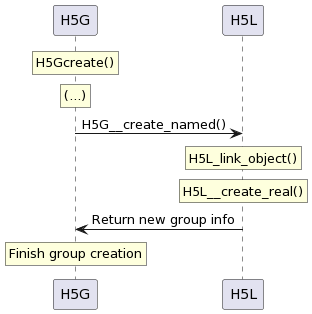
\includegraphics[width=0.40\textwidth]{images/tour_4_group_create.png}
    \caption{The library internally creates a link to a new named group}
    \label{fig:tour-4-uml-group-create}
\end{figure}

\paragraph{The Root Group} Every HDF5 file is created with a single named object - the root group. The root group has the fixed name \texttt{/}, and acts as the root of a file's hierarchy. It is the only group that does not need to reside within a group itself. The root group is closely associated with the file itself - when API functions operate on HDF5 files as objects, they often act on the root group internally.

\begin{comment}
\paragraph{Intermediate Group Creation} Figure~\ref{fig:group-intermediate-creation} shows an example of creating multiple nested groups with a single API call.

\begin{listing}
\centering
\caption{Intermediate Group Creation}
\label{lst:group-intermediate-creation}
\begin{minted}[linenos]{C}
#include "common.h"
int main() {
    hid_t file_id = H5Fcreate("group.h5", H5F_ACC_TRUNC, H5P_DEFAULTx2);
    hid_t lcpl = H5Pcreate(H5P_LINK_CREATE);
    H5Pset_create_intermediate_group(lcpl, 1);
    H5Gclose(H5Gcreate(file_id, "group1/group2/group3", lcpl,
        H5P_DEFAULTx2));
    H5Pclose(lcpl);
    H5Fclose(file_id);
    return 0;
}
\end{minted}
\end{listing}
\end{comment}

\subsection{Links}

\paragraph{Overview} The structure of an HDF5 file is a rooted, directed graph. Named objects form the nodes of this graph, and links are the edges between them. Links point from a group to a target object, and may be 'traversed' from their parent group to access the target object. Links are indexed within a group, allowing them to be iterated through recursively with \func{H5Lvisit} or non-recursively with \func{H5Literate}.

When a named object is created in a particular group, a hard link pointing to it is created and placed in that group. Hard links store the physical address of the object in the file. Other types of links, which use a name or other symbol to point to an object rather than its physical address, are called 'symbolic links'.

\paragraph{Hard Links and Objects} Each time a hard link to an object is created or destroyed, the target object's internal count of how many links point to it, the field \texttt{nlink} in the \texttt{H5O\_t} struct, is updated accordingly.

When an object has no links pointing to it, it becomes inaccessible in the file and the space it occupies is marked as 'free' by the file's free space manager. Unless persistent free space management is enabled on the file, this free space tracking information will be lost when the file is closed, and the memory will not be reclaimed until a tool such as \texttt{h5repack} is used.

In the context of HDF5, "reference count" refers to in-memory objects tracking how many other in-memory objects reference them, and the term has no relation to the number of links to an object in the file hierarchy.

\begin{comment}
https://www.plantuml.com/plantuml
@startuml
participant H5L
participant H5G
participant H5O

rnote over H5L: H5Lcreate_(hard/soft/external/ud)

alt Hard Link
rnote over H5L: H5L__create_hard
else Soft Link
rnote over H5L: H5L__create_soft
else External/User-defined Link
rnote over H5L: H5L__create_ud
end

H5L -> H5G: H5L__create_real
H5G -> H5L: H5G_traverse
H5L -> H5G: H5L__link_cb
H5G -> H5O: H5G_obj_insert

opt Hard Link
rnote over H5O: H5O_link
end
@enduml
\end{comment}

\begin{figure}
    \centering
    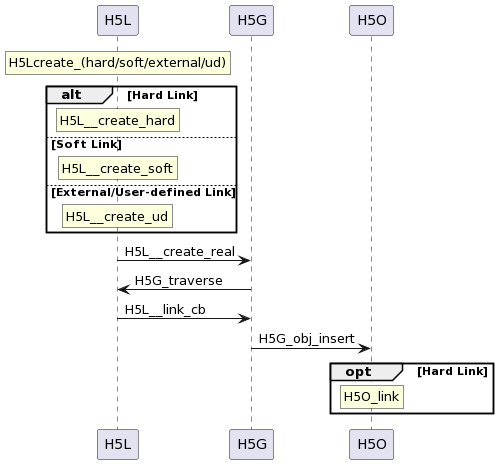
\includegraphics[width=0.6\textwidth]{images/tour_4_uml_link_create.png}
    \caption{Link creation sequence diagram}
    \label{fig:tour-4-uml-link-create}
\end{figure}

\paragraph{Link Creation} Figure~\ref{fig:tour-4-uml-link-create} illustrates the library's process for link creation. After link-type-specific setup is done by \func{H5L__create_[hard/soft/external/ud]}, the link object is created by \func{H5L__create_real}.

The API's link creation functions require both a location identifier and a name for the link that will be created. This link name may be a relative path from the object specified by the location identifier, or an absolute path from the root of the file. If the provided link name is a path with intermediate elements, then \func{H5G_traverse} is used to traverse the path and create the link object at the correct place in the file hierarchy. Once the final destination for the new link is reached, the link is inserted into the group containing it with \func{H5G_obj_insert}. If it is a hard link, \func{H5O_link} increments the target object's \texttt{nlink} count.

\paragraph{Soft Links} Soft links are a type of symbolic link that point to a path in the file hierarchy rather than an address in the file. When a soft link is created, no checks are performed to ensure that an object exists at the target path. A link that does not point to an existing object is called a dangling link. Allowing soft links to dangle means that changing, removing or entirely replacing an object that resides at a location pointed to by soft links can be done without additional work on the part of the library or the application.

\begin{listing}
\centering
\caption{Soft link example}
\label{lst:soft-link-example}
\begin{minted}[linenos]{C}

#include "common.h"
int main() {
  hid_t file_id = H5Fcreate("groups.1.h5", H5F_ACC_TRUNC, H5P_DEFAULTx2);
  hid_t group_id = H5Gcreate(file_id, "grp1", H5P_DEFAULT, H5P_DEFAULTx2);
  hid_t space_id = H5Screate(H5S_SCALAR);

  H5Lcreate_soft("/grp1/data", group_id, "link_to_data", H5P_DEFAULTx2);
  hid_t dset_id = H5Dcreate(group_id, "data", H5T_NATIVE_INT, space_id,
    H5P_DEFAULTx3);
  H5Dclose(dset_id);

  dset_id = H5Dopen(group_id, "link_to_data", H5P_DEFAULT);
  H5Dclose(dset_id);
  H5Sclose(space_id);
  H5Gclose(group_id);
  H5Fclose(file_id);
  return 0;
}

\end{minted}
\end{listing}

\begin{comment}
https://www.plantuml.com/plantuml/
@startuml
participant H5D
participant H5G

rnote over H5D: H5Dopen
H5D -> H5G: H5D__open_name

rnote over H5G: H5G_loc_find
rnote over H5G: H5G_traverse
rnote over H5G: H5G_traverse_real
group Non-Hard Link
rnote over H5G: H5G__traverse_(slink/ud)
end
rnote over H5G: H5G__loc_find_cb

H5G -> H5D: Return dataset location info
@enduml
\end{comment}

\begin{figure}
    \centering
    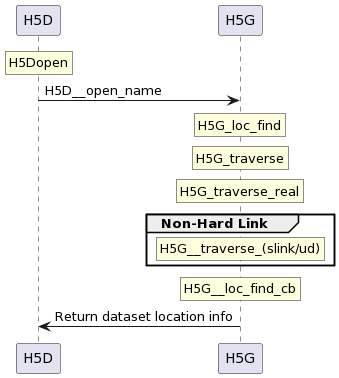
\includegraphics[width=0.40\textwidth]{images/tour_4_uml_link_access.png}
    \caption{Sequence diagram of opening a dataset through a link}
    \label{fig:tour-4-uml-link-access}
\end{figure}

\paragraph{Accessing Objects Through Links} Figure~\ref{fig:tour-4-uml-link-access} shows the process the library uses to access an object through a link.

After the VOL layer is passed through and the native \func{H5D__open_name} is invoked, \func{H5G_loc_find} is called in order to retrieve the two components of the location of the dataset - the path to it in the file hierarchy and its address in physical storage. This function invokes \func{H5G_traverse} to traverse the path to the link, as well as the path the link contains if it is a soft or external link. \func{H5G_loc_find} also provides the traversal function with the \func{H5G__loc_find_cb} callback to be used upon locating the target object. This callback copies the target object's group location information. After the location information is retrieved, the rest of the type-specific object opening work is performed.

\begin{listing}
\centering
\caption{Creating and using a user-defined link class}
\label{lst:ud-link-example}
\begin{minted}[linenos]{C}
#include <string.h>
#include "common.h"
hid_t UD_soft_traverse(const char *link_name, hid_t cur_group,
                       const void *udata, size_t udata_size,
                       hid_t lapl_id, hid_t dxpl_id) {
  const char *target_obj_name = (const char *)udata;
  hid_t ret_value = H5Oopen(cur_group, target_obj_name, lapl_id);
  return ret_value;
}

const H5L_class_t UD_soft_class[1] = {{
    H5L_LINK_CLASS_T_VERS,             /* Version number for this struct */
    (H5L_type_t)H5L_TYPE_EXTERNAL + 1, /* Link class id number.          */
    "UD_soft_link",                    /* Link class name for debugging  */
    NULL,             NULL, NULL,      /* Link class op callbacks        */
    UD_soft_traverse, NULL, NULL
}};

int main() {
  hid_t file_id = H5Fcreate("ud_link.h5", H5F_ACC_TRUNC, H5P_DEFAULTx2);
  H5Lregister(UD_soft_class);
  /* Pass the path to the root group as udata */
  H5Lcreate_ud(file_id, "ud_link", (H5L_type_t)H5L_TYPE_EXTERNAL + 1, "/",
               strlen("/") + 1, H5P_DEFAULTx2);

  hid_t group_id = H5Gopen2(file_id, "ud_link", H5P_DEFAULT);
  H5Gclose(group_id);
  H5Fclose(file_id);
  return 0;
}

\end{minted}
\end{listing}

\paragraph{User-defined Links} As part of the library's effort to be as extensible as possible, users may define and register their own link types. \func{H5Lregister} can be used to register a new link class, after which an instance of the new link class may be created with \func{H5Lcreate_ud}.

Listing ~\ref{lst:ud-link-example} shows a minimal example of a user-defined link class, which mimics the behavior of soft links. The only callback that must be defined is the traversal callback, which handles obtaining an object handle from a link pointing to that object. The other callbacks - create, move, copy, delete, and query - all have some baseline functionality implemented by the library, with the user's callback being invoked after the internal work is completed. For example, for a user-defined link class with no provided query callback, \func{H5Lget_info} will still return the character set of the link's name, its creation order in its parent group, whether its creation order is valid, and the link's type. However, the returned size of the link will default to zero unless the query operation is implemented.

\subsection{Link Storage}

\paragraph{Overview}  Similar to attributes, there are two ways that links may be stored in a file: compact and dense. Compactly stored links are kept in the object header for the group containing them, along with other metadata for that group object. Densely stored links are kept in a fractal heap. The address of the dense link fractal heap is stored in the Link Info message in the group's header, with the heap IDs to access specific dense links stored in a name index B-tree.

Older versions of the file format stored all links in a symbol table. A symbol table will still be used for link storage if the 'low' library compatibility version on a file is set lower than 1.8. By default, a new file has its 'low' compatibility version set to \texttt{H5F\_LIBVER\_EARLIEST}, which will disable use of the fractal heap for dense link storage.

Links are stored compactly if two criteria are met: the link message is under 64 KiB in size, and the number of links is below the maximum number of compact links on the group. The maximum number of compact links on a group may be set at creation time via \func{H5Pset_link_phase_change}. If either of these criteria are not met, the new link will be put into dense storage, and any existing compact links will be converted to dense storage. If the number of links later drops below the minimum number of compact links set by \func{H5Pset_link_phase_change}, then any links below 64 KiB will be converted to compact storage.

\begin{comment}
https://www.plantuml.com/plantuml/
@startuml
participant H5D
participant H5G
participant H5HF
participant H5B2

rnote over H5D: H5Dcreate
H5D -> H5G: (...)
rnote right: H5G_obj_insert

opt Fractal heap does not yet exist
rnote over H5G: H5G__dense_create
H5G -> H5HF: Create fractal heap in the file
rnote right: H5HF_create
H5G -> H5B2: Create name index B-tree
rnote right: H5B2_create

opt If creation order is tracked
H5G -> H5B2: Create creation order B-tree
rnote right: H5B2_create
end
end

rnote over H5G: H5G__dense_insert
H5G -> H5HF: Insert link into fractal heap
rnote right: H5HF_insert
H5G -> H5B2: Insert link into name B-tree
rnote right: H5B2_insert
opt If creation order is tracked
H5G -> H5B2: Insert record into creation order B-tree
rnote right: H5B2_insert
end

@enduml
\end{comment}

\begin{figure}
    \centering
    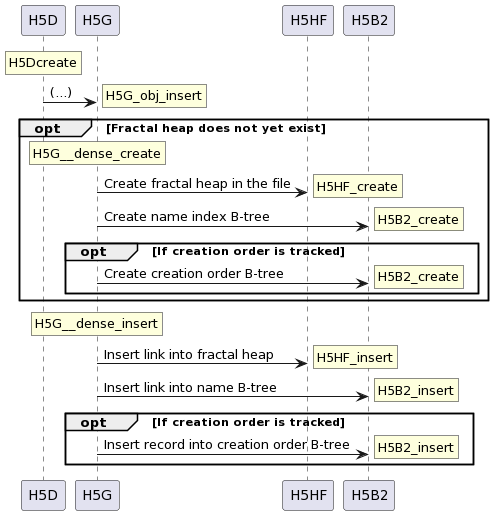
\includegraphics[width=0.6\textwidth]{images/tour_4_uml_link_storage_dense.png}
    \caption{Link insertion into dense storage during dataset creation}
    \label{fig:tour-4-uml-link-storage-dense}
\end{figure}


\begin{comment}
https://www.plantuml.com/plantuml/
@startuml
participant H5D
participant H5G

rnote over H5D: H5Dcreate
H5D -> H5G: (...)
rnote right: H5G_obj_insert

H5G -> H5O: H5G__compact_insert
rnote right: H5O_msg_create

hnote over H5O #FFAAAA: Object header is pinned
rnote over H5O: H5O_msg_append_oh
rnote over H5O: H5O__msg_alloc
rnote over H5O: H5O__copy_mesg

hnote over H5O #FFAAAA: Object header is unpinned
@enduml
\end{comment}

\begin{figure}
    \centering
    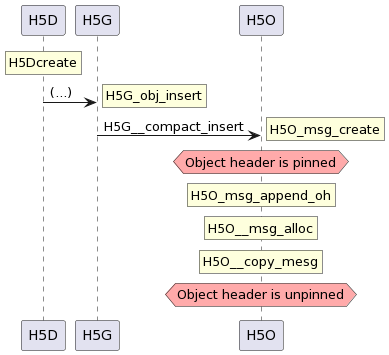
\includegraphics[width=0.5\textwidth]{images/tour_4_uml_link_storage_compact.png}
    \caption{Link insertion into compact storage during dataset creation}
    \label{fig:tour-4-uml-link-storage-compact}
\end{figure}

\paragraph{Inserting Links into Storage} An example of link insertion into dense storage is illustrated in Figure~\ref{fig:tour-4-uml-link-storage-dense}. If the file does not yet have the structures needed to store dense links, they are created in \func{H5G__dense_create}. This involves creating a fractal heap for dense links via \func{H5HF_create}, creating a B-tree to hold the names of dense links via \func{H5B2_create}, and, if creation order is tracked on the parent group, creating another B-tree to track creation order. Once the the structures for dense storage are confirmed to exist, insertion into dense storage is handled by \func{H5G_dense_insert}. The insertion into the fractal heap itself is done by \func{H5HF_insert}. The name-index B-tree stores information about the link that may later be accessed by the hash of the link name, and the creation-order B-tree stores the same information with the link creation index as the key.

\begin{comment}
https://www.plantuml.com/plantuml
@startuml
participant H5D
participant H5G
participant H5O

rnote over H5D: H5Dopen
H5D -> H5G: (...)
rnote right: H5G_traverse

group Link is compact

H5G -> H5O: H5G__compact_lookup
rnote over H5O: H5O_msg_iterate
H5O -> H5G:
rnote over H5G: H5G__compact_lookup_cb
H5G -> H5O: If link found by name
end
rnote over H5O: H5O_msg_copy
H5O -> H5G: Return link info
H5G -> H5D: Return dataset handle
@enduml
\end{comment}

\begin{figure}
\centering
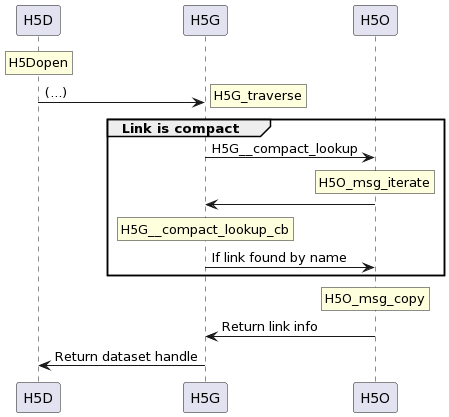
\includegraphics[width=0.55\textwidth]{images/tour_4_uml_link_access_compact.png}
\caption{How the library accesses a compact link}
\label{fig:tour-4-uml-link-access-compact}
\end{figure}

\begin{comment}
https://www.plantuml.com/plantuml
@startuml
participant H5D
participant H5G
participant H5O
participant H5HF
participant H5B2

rnote over H5D: H5Dopen
H5D -> H5G: (...)
rnote right: H5G_traverse

group Link to dataset is dense
rnote over H5G: H5G__dense_lookup
H5G -> H5HF: Open fractal heap of file
rnote right: H5HF_open

H5G -> H5B2: Open name index B-tree
rnote right: H5B2_open
H5G -> H5B2: Search for link name in B-tree
rnote right:H5B2_find

H5B2 -> H5G: If dense link is found by name
rnote over H5G: H5G__dense_lookup_cb
H5G -> H5O: Copy link message from header
end

rnote over H5O: H5O_msg_copy
H5O -> H5G: Return link info
H5G -> H5D: Return dataset handle
@enduml
\end{comment}

\begin{figure}
\centering
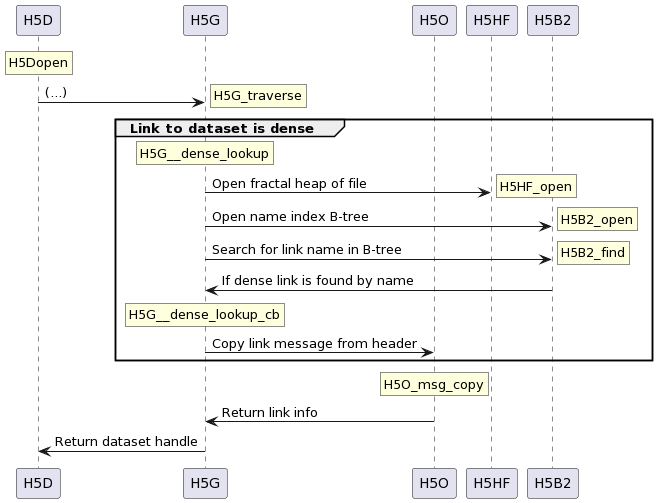
\includegraphics[width=0.70\textwidth]{images/tour_4_uml_link_access_dense.png}
\caption{How the library accesses a dense link}
\label{fig:tour-4-uml-link-access-dense}
\end{figure}

The process for compact link insertion into the object header is illustrated in Figure~\ref{fig:tour-4-uml-link-storage-compact}. Compact links are inserted by \func{H5G__compact_insert}. \func{H5G_msg_create} sets up the message to be inserted. Before the message is appended onto the object header, the object header is "pinned" with \func{H5O_pin}. Pinning the object header prevents it from being written from cache to storage in the middle of operations that modify the header. \func{H5O_msg_append_oh} appends the newly created message to the object header. This is done in two parts: first \func{H5O__msg_alloc} creates space in the object header, then \func{H5O__copy_mesg} populates the allocated memory with link message information. Lastly, the object header is unpinned by \texttt{H5O\_unpin()}, allowing it to be flushed from cache again.

\paragraph{Accessing Links in Storage} Figures~\ref{fig:tour-4-uml-link-access-compact} and \ref{fig:tour-4-uml-link-access-dense} illustrate the library's process for accessing objects through links in compact and dense storage, respectively.

\func{H5G_traverse} is used regardless of storage type to locate the link through the provided path in the file hierarchy. Once the correct location in the hierarchy is reached, the process branches based on how the link is stored.

If the link is compact, \func{H5G__compact_lookup} searches the object header for a message describing a link of the correct name. \func{H5O_msg_iterate} iterates through each message and uses \func{H5G_compact_lookup_cb} to copy the link information if a match is found.

If the link is dense, \func{H5G__dense_lookup} does the name lookup. The dense link fractal heap and the name index B-tree are both opened. \func{H5B2_find} searches name index B-tree for the dense link. If a match is found, the provided callback \func{H5G__dense_lookup_cb} copies the link information.

In both cases, once the link is found by name, its information is copied with \func{H5O_msg_copy} and returned to \func{H5G_traverse}. The link traversal callback for the link's type is used to access information about the object through the link, and a handle to the object is returned by the top-level open function.

\subsection{Summary} Implementing group membership via links introduces a layer of indirection to the file hierarchy which is extremely powerful. Based on the use case of the application, objects can be accessed based on storage location, path within the file hierarchy, path in the filesystem via external links, or something else entirely with user-defined link classes. Since scalability with extremely large amounts of data is a core goal of the HDF5 library, maximizing the user's ability to manipulate the file hierarchy without affecting the underlying arrangement of data is critical.

Scalability with large numbers of links in a group was another important design goal, realized in the architecture by dense link storage. The tradeoff between compact storage being better for small numbers of links and dense storage being better for large numbers of links is automatically handled during operation by the maximum compact/minimum dense thresholds, and may also be custom-fit to a use case by the user through manipulating property lists.


\section{Stoked on datatypes}\label{sec:tour5}

%|  Name  | TODO | ONGOING | DONE |
%|--------|------|---------|------|
%| Dana   | x    |         |      |
%| Gerd   | x    |         |      |
%| Glenn  |      |         |  x   |
%| Jordan | x    |         |      |
%| Luke   | x    |         |      |
%| Matt   |      |         | x    |
%| Neil   | x    |         |      |
%| Scot   | x    |         |  x    |

%\todo[inline]{Owner: Matt -- Priority: High -- Effort: M - Completion: 100\%}
Continuing in the educational tours, we will delve into the intricate details of datatypes, their categories, and how they are represented and managed by the HDF5 library. We will also explore the encoding process of datatypes for disk storage and how the library handles data of different data types in the file.

 Moreover, we will also highlight the remarkable extensibility and customizability of the HDF5 library, which empowers users to define their own datatypes, composite datatypes, and datatype conversion functions. This capability allows for optimizing almost every I/O process step.
\subsection{Datatype life cycle}

Speaking broadly, the datatype life cycle begins at build configuration time with the discovery of platform-specific types, proceeds at run-time during library initialization, and continues with the construction of predefined and user-defined datatypes. In this section, we describe the library infrastructure supporting this process.

\paragraph{Configuration-Time Type Discovery} The HDF5 library checks the size of each built-in C type on the current platform at configuration time. A set of macros with names of the form \texttt{H5\_SIZEOF\_<TYPE>} will be defined in the generated file \texttt{H5pubconf.h}. These macros define an internal assignment operator between numeric types that works regardless of the types' relative sizes, \texttt{H5\_CHECKED\_ASSIGN}.

\paragraph{Predefined Datatypes} The types predefined by the library have standard symbolic names of the form \texttt{H5T\_<arch>\_<base>} where 'arch' is an architecture name, and 'base' is a programming type name formed from a letter for the type class, a number for the precision in bits, and an indication of byte order. For example, \texttt{H5T\_INTEL\_I64BE} is a predefined type for 64-bit big-endian integers on Intel CPUs.

The names through which the predefined types are accessed are defined as macros in \texttt{H5Tpublic.h}. The macro \texttt{H5T\_<TYPE>} evaluates to \texttt{H5OPEN H5T\_<TYPE>\_g}. \texttt{H5OPEN} is a macro that ensures the library is initialized if the type macro was used in a public or user application file. \texttt{H5T\_<TYPE>\_g} is a globally accessible handle ID for the predefined type.

Predefined types' inability to be modified is implemented through the \texttt{state} field of \texttt{H5T\_t}'s shared information. Predefined types are created with their state set to immutable, making them unmodifiable and unable to be closed by the user.

\paragraph{Predefined Datatype Initialization} The H5T package is initialized during phase 2 of H5VL's initialization, as seen in Listing~\ref{lst:vol2-init-table}. An internal diagram of \func{H5T_init} is shown in Figure~\ref{fig:h5t-init-table}.

Predefined types that match the native platform are created first in two steps. In the first step, predefined float datatypes that match the native platform are created and registered in \\ \func{H5T__init_native_float_types}. The \texttt{DETECT\_F} macro detects the native platform's floating-point properties, which are used to construct matching datatypes. The datatypes are assigned library handles by \texttt{H5I\_register()}. These handles are stored in a set of global variables with names of the form \texttt{H5T\_NATIVE\_<TYPE>\_g}. In the second step, a similar process is carried out for all other native datatypes in \texttt{H5T\_\_init\_native\_internal()}, using detected information about the platform's byte order and alignment.

Once the predefined native datatypes are created, they are used to create the predefined non-native datatypes through the macro \texttt{H5T\_INIT\_TYPE}. If the new type to be constructed is based on an existing one, this macro copies the provided base type with \texttt{H5T\_copy()} before making size and byte order modifications. If the new type is not based on an existing type, the macro directly allocates space for a new \texttt{H5T\_t} structure and populates it using another macro of the form \texttt{H5T\_INIT\_TYPE\_<TYPE>\_CORE}. In both cases, \texttt{H5T\_INIT\_TYPE} registers the newly created datatype with the library, assigns it a handle through \texttt{H5I\_register()}, and makes the handle globally accessible through \texttt{H5T\_<ARCH>\_<BASE>\_g}. A user can then access these handles through macros of the form \texttt{H5T\_<ARCH>\_<BASE>}, as discussed in the previous section.

In addition to initializing predefined datatypes, \func{H5T_init} also sets up many internal datatype conversion routines through \func{H5T__register_int}, and registers the default property list for datatype creation, \texttt{H5P\_DATATYPE\_CREATE}, through \texttt{H5P\_create\_id()}.

\begin{comment}
http://www.plantuml.com/plantuml/uml/
@startuml
participant H5T
participant H5I
participant H5P

rnote over H5T: H5T_init
group Create native predefined dtypes
rnote over H5T: H5T__init_native_float_types
H5T -> H5I:
rnote over H5I: H5I_register

rnote over H5T: H5T__init_native_internal
H5T -> H5I:
rnote over H5I: H5I_register
end

group For each non-native predefined dtype
H5T -> H5I: H5T_INIT_TYPE
rnote over H5I: H5I_register
end

rnote over H5T: H5T__register_int
H5T -> H5P: Register dtype creation plist
rnote right: H5P_create_id
@enduml
\end{comment}

\begin{figure}
\centering
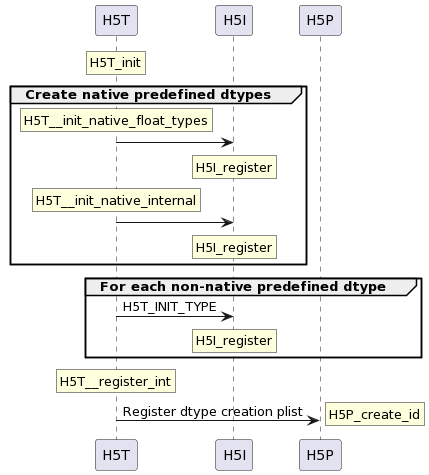
\includegraphics[width=0.55\textwidth]{images/tour_5_uml_h5t_init.png}
\caption{A sequence diagram for \texttt{H5T\_init}}
\label{fig:h5t-init-table}
\end{figure}

\paragraph{User-defined Datatypes} Users may derive their own types from the predefined types by copying them to get a transient, modifiable copy. Figure~\ref{fig:predefined-type-copy} is a minimal example demonstrating user-defined type creation. Figure~\ref{fig:tour-5-uml-datatype-copy} shows the internal operation of \func{H5Tcopy}.

\begin{figure}
\centering
\caption{Creation of a user-defined type identical to a platform-native integer.}
\label{fig:predefined-type-copy}
\begin{minted}[linenos]{C}
int main(void) {
    hid_t type_id = H5Tcopy(H5T_NATIVE_INT);
    H5Tclose(type_id);
};

\end{minted}
\end{figure}

\begin{comment}
http://www.plantuml.com/plantuml/uml/
@startuml
participant H5T
participant "H5T Private" as private
participant H5O
participant H5I

rnote over H5T: H5Tcopy
H5T -> private: H5T_copy (Transient)
rnote over private: H5T__initiate_copy
rnote over private: H5T__complete_copy

H5T -> H5I: Register newly opened datatype object with the library
rnote over H5I: H5I_register()
H5I -> H5T: Datatype handle ID
@enduml
\end{comment}

\begin{figure}
    \centering
    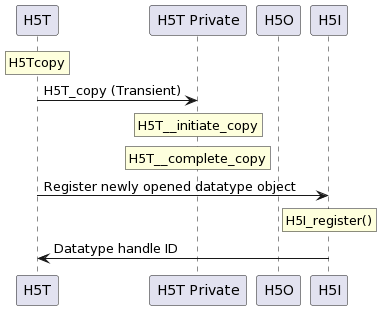
\includegraphics[width=0.5\textwidth]{images/tour_5_uml_datatype_copy.png}
    \caption{H5Tcopy sequence diagram}
    \label{fig:tour-5-uml-datatype-copy}
\end{figure}

\texttt{H5Tcopy} performs the datatype copy operation in two steps. First, \texttt{H5T\_\_initiate\_copy()} allocates in-memory structures for the new object and, if the original datatype is committed, increases its in-memory reference count. Then \texttt{H5T\_\_complete\_copy()} copies the information for the new datatype from the old datatype. Lastly, \texttt{H5I\_register()} assigns a handle ID to the new datatype.

\begin{listing}
\centering
\caption{Committing a type as an HDF5 Object in storage}
\label{lst:type-commit}
\begin{minted}[linenos]{C}
int main(void) {
    hid_t file_id = H5Fcreate("type_test.h5", H5F_ACC_TRUNC, H5P_DEFAULTx2);
    hid_t type_id = H5Tcopy(H5T_NATIVE_INT);

    H5Tcommit(file_id, "user_defined_integer", type_id, H5P_DEFAULTx3);

    H5Tclose(type_id);
    H5Fclose(file_id);
};

\end{minted}
\end{listing}

\begin{comment}
http://www.plantuml.com/plantuml/uml/
@startuml
participant H5T
participant H5L

rnote over H5T: H5Tcommit
rnote over H5T: (...)

rnote over H5T: H5T_copy
H5T -> H5L: H5T__commit_named
rnote over H5L: H5L_link_object

rnote over H5T: New committed type object \nis attached to original H5T_t
@enduml
\end{comment}

\begin{figure}
\centering
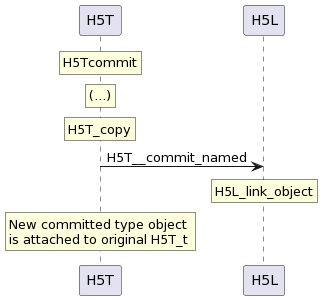
\includegraphics[width=0.4\textwidth]{images/tour_5_uml_datatype_commit.png}
\caption{Internal operation of H5Tcommit}
\label{fig:tour-5-uml-datatype-commit}
\end{figure}

\paragraph{Committed Datatypes} There are two kinds of datatypes: transient datatypes that exist only in memory and committed (formerly "named") datatype objects that are written to storage.

Listing~\ref{lst:type-commit} shows a minimal program that turns a transient datatype into a committed datatype via \\ \func{H5Tcommit}. After data is written to the file, the datatype will exist as an object on the file in storage.

Figure~\ref{fig:tour-5-uml-datatype-commit} shows the internal work done by \func{H5Tcommit} when using the native VOL. A copy of the provided datatype is created by \func{H5T_copy}, and this copy is written to storage. \func{H5T__commit_named} sets up creation information for \func{H5L_link_object}, which creates the committed datatype object and a hard link used to link it into the file hierarchy. Lastly, the newly committed datatype object is attached as an \texttt{H5VL\_object\_t} instance to the \texttt{vol\_obj} field of the original datatype provided to \texttt{H5Tcommit()}.

\subsection{Datatype conversion}\label{sec:dtype-conv}

In this section, we describe the circumstances in which and where datatype conversion takes place during user data transfer and how the library locates appropriate datatype conversion functions at run-time.

\paragraph{Overview} Datatype conversion is performed at transfer (read or write) time. Which conversions are possible depends on the set of defined conversion functions. As a rule of thumb, conversion is possible if the datatypes of the source and destination are different types within the same datatype class. For example, integers can generally be converted to other integers and floats to other floats. Some other common conversions, like integer-to-float and vice versa, are also predefined.

\paragraph{Conversion Functions} Conversion between a source and destination type is performed via a conversion function. A conversion function may be 'hard' or 'soft'. Hard conversion functions are each associated with a particular source and destination datatype, while soft conversion functions are related to entire datatype classes.

The library maintains a global table of type conversion functions, \texttt{H5T\_g}. Each conversion function is uniquely identified by a ``path'' (\texttt{H5T\_path\_t}) formed from the source and destination datatypes. When a conversion is necessary, a binary search is performed on this table to locate an appropriate conversion function.

\paragraph{User-Defined Conversion Functions} Users can add new conversion functions or overwrite the behavior of existing conversion functions through \func{H5Tregister}. A new hard conversion function will overwrite any previous conversion functions for the specified types, and a new soft conversion function will overwrite the conversion functions for any types to which it is applicable that do not already have a hard conversion function.

\begin{listing}
\centering
\caption{User-defined datatype conversion -- setup.}
\label{lst:ud-datatype-conversion-setup}
\begin{minted}[linenos]{C}
#include "common.h"

typedef struct src_t {
     uint32_t a;
     float b;
  } src_t;

typedef struct dst_t {
     float b;
  } dst_t;

herr_t convert(hid_t src_id, hid_t dst_id, H5T_cdata_t *cdata,
    size_t nelmts, size_t buf_stride, size_t bkg_stride, void *buf,
    void *bkg, hid_t dxpl)
{
  herr_t retval = EXIT_SUCCESS;
  switch (cdata->command)
  {
  case H5T_CONV_INIT:
    printf("Initializing conversion function...\n");
    break;
  case H5T_CONV_CONV:
    printf("Converting...\n");
    for (size_t i = 0; i < nelmts; ++i)
      ((dst_t*) buf)[i].b = ((src_t*) buf)[i].b;
    break;
  case H5T_CONV_FREE:
    printf("Finalizing conversion function...\n");
    break;
  default:
    break;
  }
  return retval;
}
\end{minted}
\end{listing}

Listing~\ref{lst:ud-datatype-conversion-setup} shows a user-defined conversion function \func{convert}, which converts between the user-defined compound datatypes \texttt{src\_t} and \texttt{dst\_t}. Notice that the conversion operation, \texttt{H5T\_CONV\_CONV}, occurs entirely within the main buffer. This is straightforward in this case because \texttt{src\_t} is larger than \texttt{dst\_t}, and so the assignment to \texttt{((dst\_t*) buf)[i].b} will never overwrite any memory needing to be read to convert a subsequent element. More complex conversions may need to use the 'background buffer', \texttt{bkg}, as a place for temporary storage.

\begin{listing}
\centering
\caption{User-defined datatype conversion -- invoked directly.}
\label{lst:ud-datatype-conversion-direct}
\begin{minted}[linenos]{C}
int main() {
  hid_t src = H5Tcreate(H5T_COMPOUND, sizeof(struct src_t));
  H5Tinsert(src, "a", HOFFSET(struct src_t, a), H5T_NATIVE_UINT32);
  H5Tinsert(src, "b", HOFFSET(struct src_t, b), H5T_NATIVE_FLOAT);
  hid_t dst = H5Tcreate(H5T_COMPOUND, sizeof(struct dst_t));
  H5Tinsert(dst, "b", HOFFSET(struct dst_t, b), H5T_IEEE_F32LE);
  H5Tregister(H5T_PERS_SOFT, "src_t->dst_t", src, dst, &convert);
  struct src_t buf[] = {
    {1, 1.0} , {2, 2.0}, {3, 3.0}, {4, 4.0} , {5, 5.0} };
  H5Tconvert(src, dst, 5, buf, NULL, H5P_DEFAULT);

  H5Tunregister(H5T_PERS_SOFT, "src_t->dst_t", src, dst, &convert);
  H5Tclose(dst);
  H5Tclose(src);
  return 0;
}
\end{minted}
\end{listing}

\begin{listing}
\centering
\caption{User-defined datatype conversion -- invoked implicitly during write.}
\label{lst:ud-datatype-conversion-implicit}
\begin{minted}[linenos]{C}
#include "common.h"
herr_t convert_float(hid_t src_id, hid_t dst_id, H5T_cdata_t *cdata,
    size_t nelmts, size_t buf_stride, size_t bkg_stride, void *buf,
    void *bkg, hid_t dxpl)
{
  herr_t retval = EXIT_SUCCESS;
  switch (cdata->command)
  {
  case H5T_CONV_INIT:
    printf("Initializing float conversion function...\n");
    break;
  case H5T_CONV_CONV:
    printf("Converting floats...\n");
    for (size_t i = 0; i < nelmts; ++i)
      ((float*) buf)[i] = ((double*) buf)[i];
    break;
  case H5T_CONV_FREE:
    printf("Finalizing float conversion function...\n");
    break;
  default:
    break;
  }
  return retval;
}

int main() {
  hid_t src = H5Tcopy(H5T_NATIVE_DOUBLE);
  hid_t dst = H5Tcopy(H5T_NATIVE_FLOAT);
  H5Tregister(H5T_PERS_SOFT, "double->float", src, dst, &convert_float);
  double buf[] = {1.0, 2.0, 3.0, 4.0, 5.0};

  hid_t file_id = H5Fcreate("float_conv.h5", H5F_ACC_TRUNC, H5P_DEFAULTx2);
  hid_t space_id = H5Screate_simple(1, (const hsize_t[]) {5}, NULL);
  hid_t dset_id = H5Dcreate(file_id, "dset", dst, space_id, H5P_DEFAULTx3);
  H5Dwrite(dset_id, src, space_id, H5S_ALL, H5P_DEFAULT, buf);
  H5Tunregister(H5T_PERS_SOFT, "double->float", src, dst, &convert_float);
  H5Fclose(file_id);
  H5Dclose(dset_id);
  H5Tclose(dst);
  H5Tclose(src);
  return 0;
}
\end{minted}
\end{listing}

\begin{comment}
http://www.plantuml.com/plantuml/uml/
@startuml
participant H5T
participant H5D

rnote over H5D: H5Dwrite
rnote over H5D: H5D__write
group Initialize type info for transfer
rnote over H5D: H5D__typeinfo_init
rnote over H5D: H5D__typeinfo_init_phase2
rnote over H5D: H5D__typeinfo_init_phase3
end
rnote over H5D: H5D__contig_write
H5D -> H5T: H5D__scatgath_write
rnote over H5T: H5T_convert
rnote over H5T: User conversion callback
@enduml
\end{comment}

\begin{figure}
    \centering
    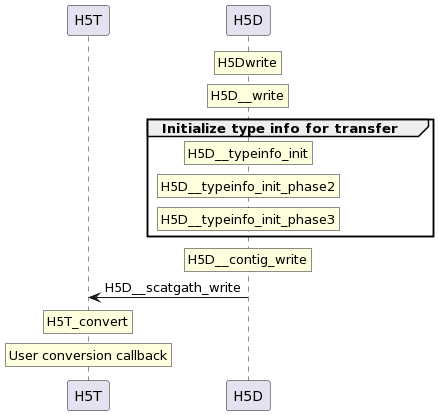
\includegraphics[width=0.50\textwidth]{images/tour_5_uml_datatype_conversion.png}
    \caption{Datatype conversion with user callback diagram}
    \label{fig:tour-5-uml-datatype-conversion}
\end{figure}

Listing~\ref{lst:ud-datatype-conversion-direct} creates compound datatypes corresponding to \texttt{src\_t} and \texttt{dst\_t}, and registers \texttt{convert()} as a soft conversion function from\texttt{src} to \texttt{dst}. It invokes the library's top-level conversion function \texttt{H5Tconvert()}, automatically finding the newly registered conversion function by a path.

Datatype conversion can also be done automatically by the library during writes or reads. Listing~\ref{lst:ud-datatype-conversion-implicit} shows an example of a program where a user-defined conversion between floats is done automatically during a write to a dataset.

Figure~\ref{fig:tour-5-uml-datatype-conversion} illustrates how type conversion happens during a write to a dataset. The library's internal dataset write function \func{H5D__write} initializes datatype information in three phases. The initialization is done in phases due to requirements imposed by parallel I/O. Specifically, when doing parallel I/O, the maximum datatype size across all destination objects must be computed after the first phase, and the selection in the destination datasets must be adjusted after the second phase.

The first phase of type info initialization, \func{H5D_typeinfo_init}, populates the \texttt{type\_info} field of each dataset's \texttt{H5D\_dset\_io\_info\_t} structure with the appropriate datatype conversion function, the size of each datatype, and whether this is the special case of converting between compound datatypes that are subsets of one another. Unlike the other phases, the first phase is done separately for each destination dataset.

The second phase, \func{H5D__typeinfo_init_phase2}, checks if selection I/O can be used and if the (expected) size of the conversion buffer and background buffer are sufficient to perform the conversion with the given selection.

The third and final phase, \func{H5D__typeinfo_init_phase3}, allocates a type conversion buffer and a background buffer of appropriate size for each dataset that requires them and did not have them provided through transfer properties.

After the type info for the transfer is fully initialized, the write proceeds through a write callback specific to the layout of the target dataset(s). For example, for the program in Listing~\ref{lst:ud-datatype-conversion-implicit}, the dataset's layout is \texttt{H5D\_CONTIGUOUS}, and so the write callback is \texttt{H5D\_\_contig\_write()}. To gather elements from the user-provided buffer for contiguous writes to disk, \texttt{H5D\_\_scatgath\_write()} is invoked. Type conversion is then performed in the provided buffers right before the data is scattered to the file.


\subsection{Datatype metadata \& value encodings}


In this section, we describe the datatype metadata retained in the HDF5 library and files, how the values of certain non-fixed-size datatypes are represented and encoded, and how the datatype affects where encoded values are stored in the HDF5 file.

\paragraph{Overview of Datatype Metadata Storage} An HDF5 file is stored on disk as a global heap and data objects (among other things outside the scope of this section). Each data object has an 'object header' and 'object information.' The object information is the user's stored data, e.g., scientific measurements. The object header contains 'messages' which describe metadata regarding the information object.

Datatypes exist on disk as Datatype Messages according to the HDF file format. A Datatype Message contains information about the datatype's size, class, and class-specific properties.

Transient datatypes are not written to disk unless they are used to create attributes or datasets. In this case, the object header for the attribute or dataset will contain a Datatype Message describing the datatype.

Recall that committed datatypes must be linked into the file hierarchy. A committed datatype is stored on disk as an object header with a Datatype Message. If a committed datatype is used in a dataset or an attribute, then the Datatype Message for that dataset or attribute contains a pointer to the original committed datatype's Datatype Message - the information is not duplicated.


% \paragraph{Datatype Metadata} A file retains the metadata about a datatype necessary to reconstruct it when reading from the file. The first 8 bytes of a Datatype Message describe the class of the datatype, the size of an instance of the datatype, and some class-specific flags. Because 4 bytes (32 bits) in the message are for the size of a datatype instance, a single element in a dataset or attribute cannot be larger than $2^{32} -1 \approx $ 4 gigabytes. After the first 8 bytes of the message is a properties section without a fixed length, which contains information specific to each datatype class. The specifics of these properties are detailed in the file format documentation.

\paragraph{Datatype Encoding} Datatype encoding is the process of converting an in-memory datatype object (\texttt{H5T\_t}) to a series of bytes which may be written to storage as a Datatype Message. This process may be invoked explicitly by \texttt{H5Tencode()/H5Tdecode()} or implicitly when writing objects with a datatype to storage.

Figure~\ref{fig:tour-5-uml-datatype-encode} shows the library's datatype encoding process. Some internal routines require a valid \texttt{H5F\_t} file struct but do not modify or depend on a real external file. To support datatype encoding/decoding without a real associated file, \texttt{H5F\_fake\_alloc()} creates a 'fake' file struct with no counterpart in storage. The size of the message to create is determined by \texttt{H5O\_msg\_raw\_size()}, which invokes the Datatype Message class's  'size' callback, \texttt{H5O\_\_dtype\_size()}. Similarly, the generic \texttt{H5O\_msg\_encode()} invokes the Datatype Message class's encode callback, \texttt{H5O\_\_dtype\_encode()}. This encode callback populates the provided buffer with information from the datatype. Suppose the datatype is non-atomic; recursive calls to \texttt{H5O\_\_dtype\_encode\_helper()} populate each component datatype. For compound types, a separate recursive call encodes each member field. A single recursive call is used to encode the base type for arrays, variable-length types, and enums.

\begin{comment}
http://www.plantuml.com/plantuml/
@startuml
rnote over H5T: H5Tencode
rnote over H5T: H5T_encode

H5T -> H5F: Get fake file struct
rnote over H5F: H5F_fake_alloc

H5T -> H5O: Compute msg size
rnote over H5O: H5O_msg_raw_size
rnote over H5O: H5O__dtype_size

H5T -> H5O: Encode dtype to msg recursively
rnote over H5O: H5O_msg_encode
rnote over H5O: H5O__dtype_encode
rnote over H5O: H5O__dtype_encode_helper

opt Non-atomic dtype
rnote over H5O: Recursive call(s)
rnote over H5O: H5O__dtype_encode_helper
end
@enduml
\end{comment}

\begin{figure}
    \centering
    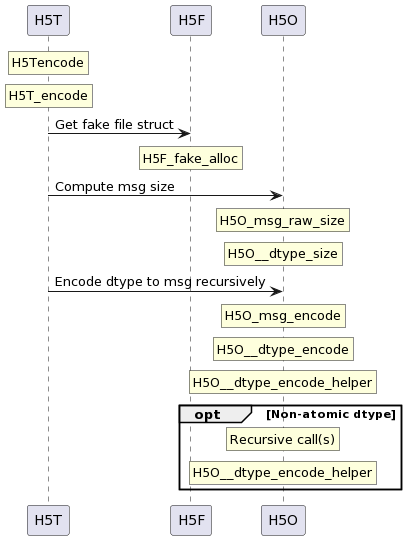
\includegraphics[width=0.45\textwidth]{images/tour_5_uml_datatype_encode.png}
    \caption{Datatype encoding process}
    \label{fig:tour-5-uml-datatype-encode}
\end{figure}

\paragraph{Datatype storage} Data with a simple atomic datatype is stored in the object information section of the data object. Because elements of more complex datatypes may have an indeterminate or variable size, they must be stored differently. Variable-length and region reference data are stored in the file's global heap. Object reference data is stored as the offsets necessary to read from the object header of the referenced object. Compound datatype elements are stored as a contiguous stream of the structure's items, each formatted according to its datatype.

\subsection{Summary}

In this tour, we covered the different categories of datatypes, how they are represented and handled by the library, and how objects use them. We reviewed how datatypes are encoded for storage on disk and how data of different datatypes is stored in the file.

The ability for the user to define their own datatypes, composite datatypes, and datatype conversion functions is another example of the extensibility and customizability of the HDF5 library, allowing users to optimize nearly every step in the I/O process.


\section{Getting down and dirty with caches}\label{sec:tour6}

%|  Name  | TODO | ONGOING | DONE |
%|--------|------|---------|------|
%| Dana   | x    |         |      |
%| Gerd   |      |         | x    |
%| Glenn  |      |         |   x  |
%| Jordan | x    |         |      |
%| Luke   | x    |         |      |
%| Matt   |      |         |  x   |
%| Neil   | x    |         |      |
%| Scot   |     |         |   x   |

%\todo[inline]{Owner: Gerd -- Priority: High -- Effort: M -- Completion: 100\%}

Throughout this tour, we describe the different user-controllable caching and buffering facilities. Figure~\ref{fig:cache-buf} shows an overview of these facilities.

\begin{figure}[bh]
\centering
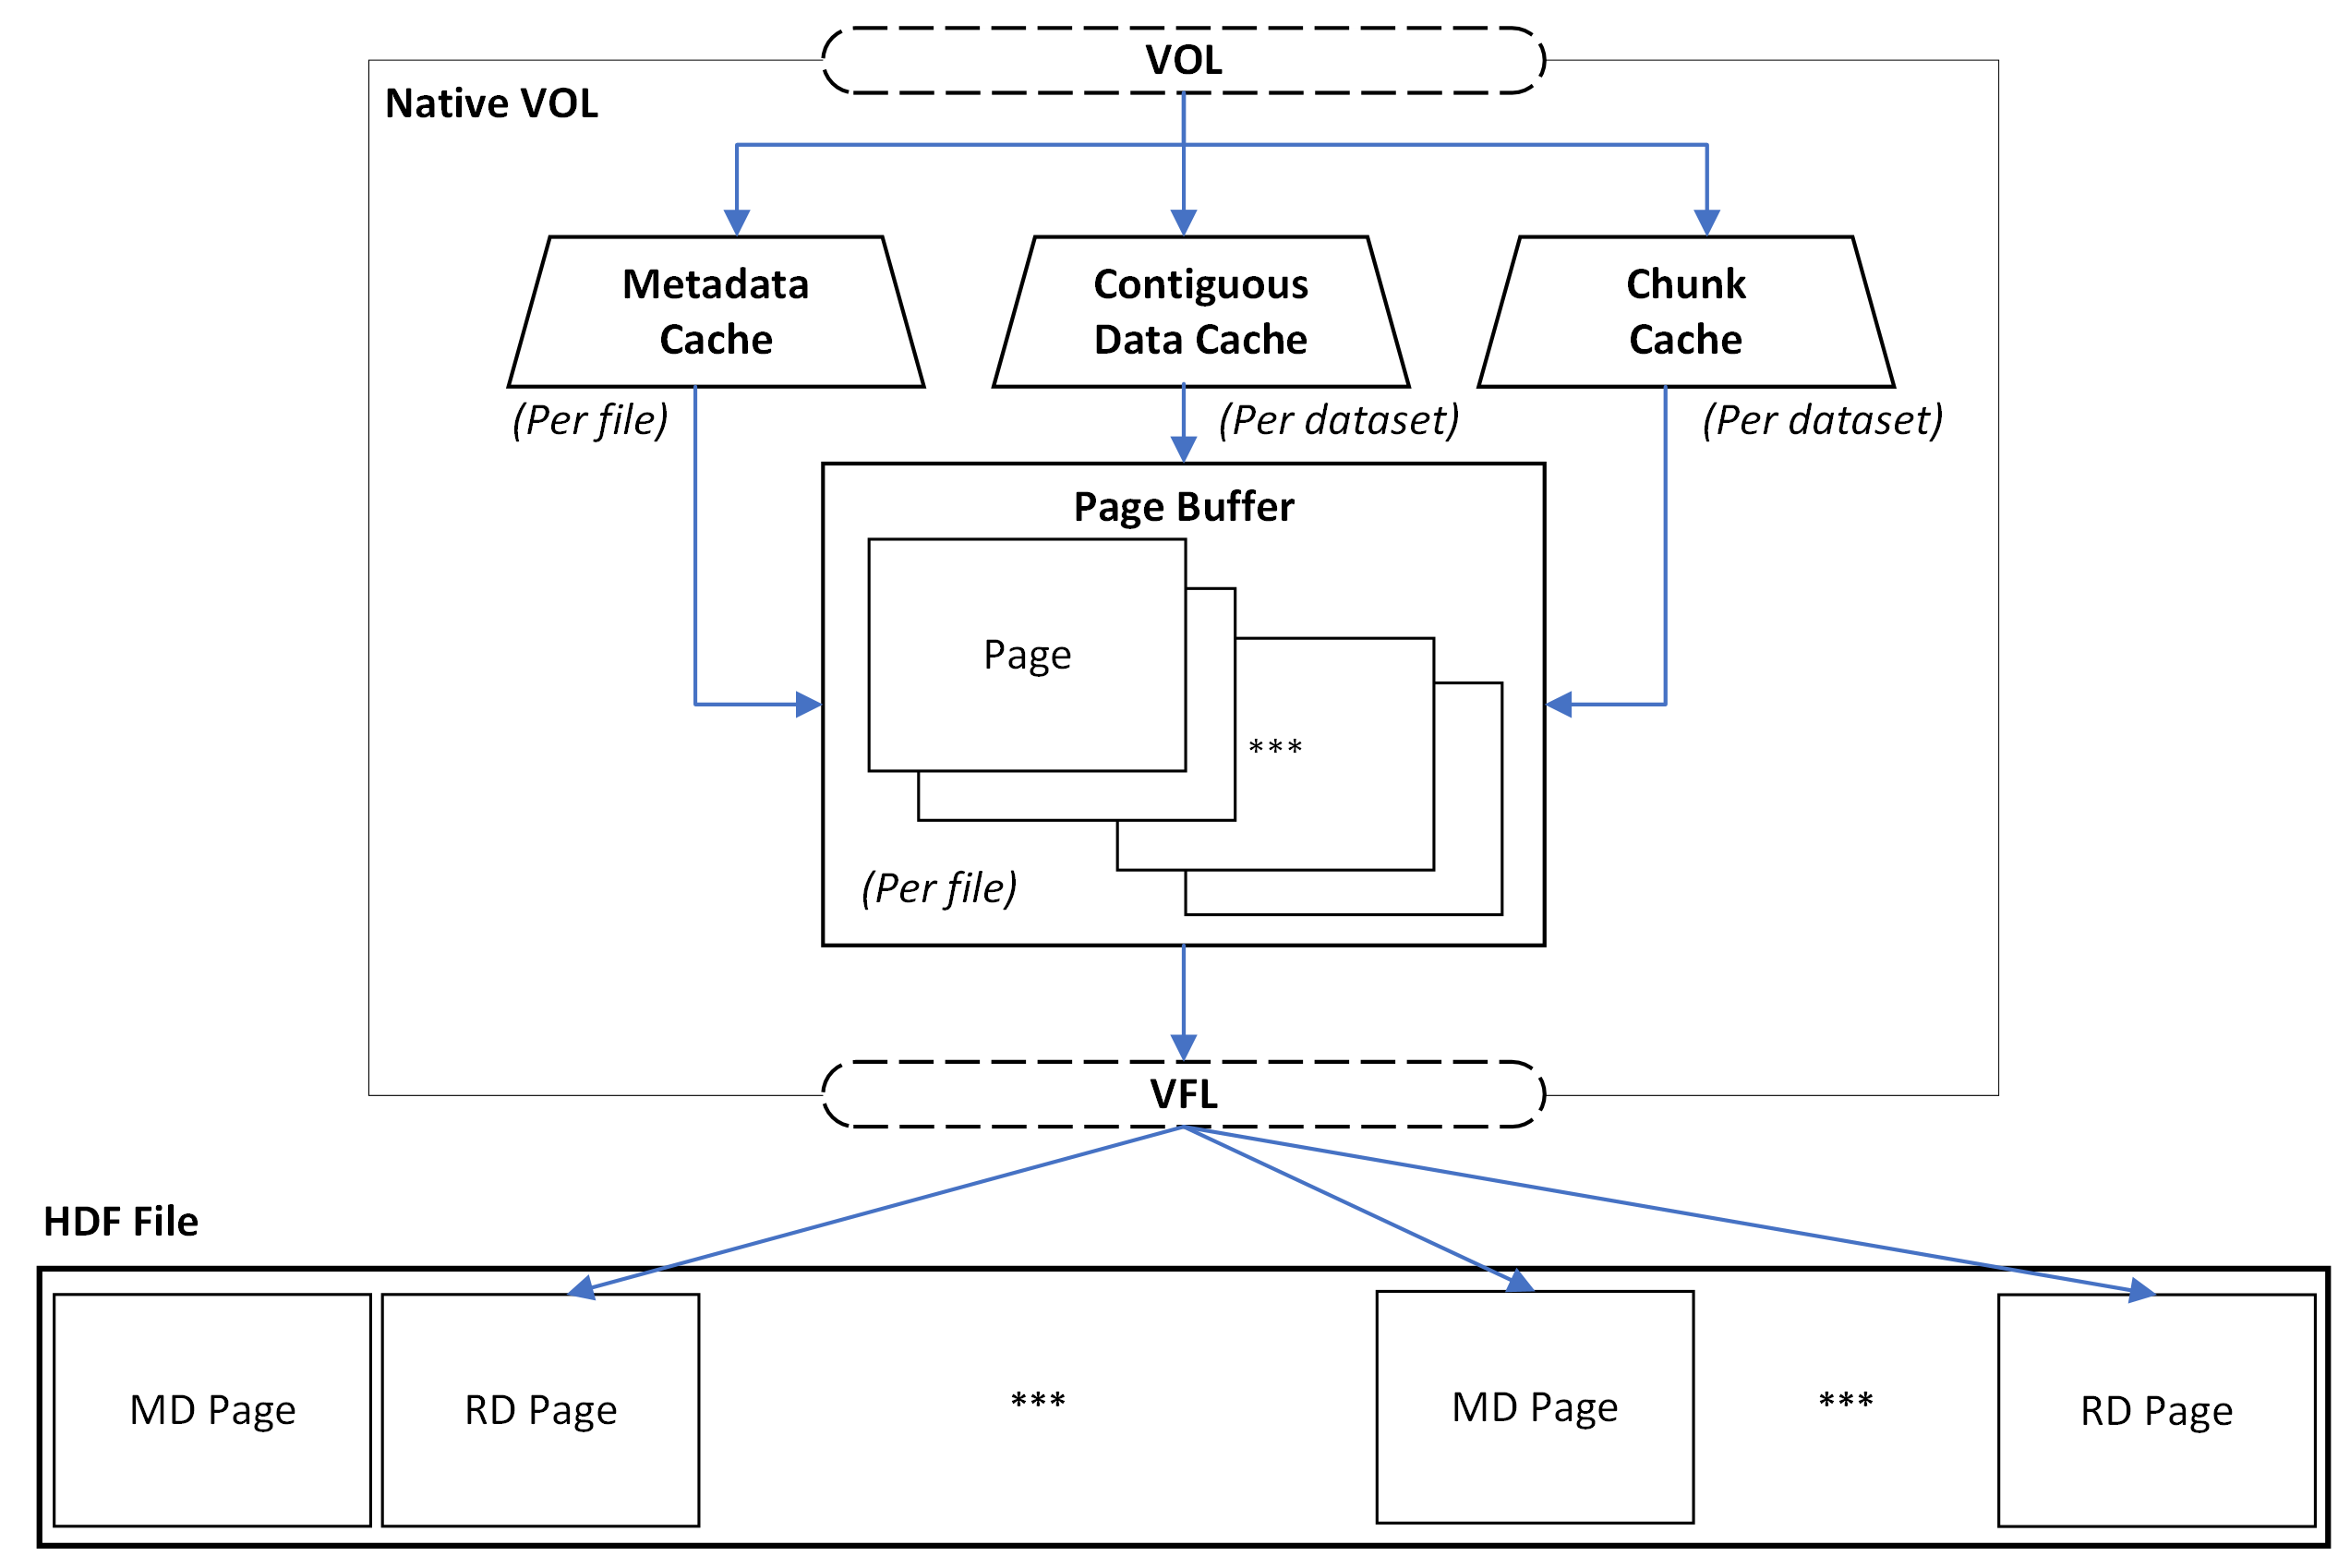
\includegraphics[width=\textwidth]{images/Caches to caches.png}
\caption{Native VOL caching and buffering.}
\label{fig:cache-buf}
\end{figure}

There are four architectural elements in the native VOL that implement caching or buffering functionality.

\begin{itemize}
    \item \textbf{Metadata cache:} We have encountered the metadata cache in Sections~\ref{sec:tour2} and~\ref{sec:tour3}.
    \item \textbf{Contiguous data cache:}  Frequently accessed contiguous dataset regions can be held in memory to minimize small I/O for datasets with contiguous storage layouts.
    \item \textbf{Chunk cache:} Frequently accessed chunks can be held in memory to minimize chunk I/O for datasets with chunked storage layouts.
    \item \textbf{Page buffer:} Since HDF5 library version 1.10.0, file space can be managed and I/O operations performed in fixed-size pages. This so-called `paged aggregation' or `paged allocation' scheme is most effective when combined with a page buffer.
\end{itemize}

The cache vs. buffer terminology in the native VOL is a little murky. The term `cache' is usually applied to a data structure that, in its implementation, uses several slots to which specific entries are assigned and which is controlled by a hash function that might have a degree of associativity. Typically, there is also an entry eviction or prefetch policy defined. The metadata and chunk caches are caches in that sense. The contiguous data cache (or sieve buffer), not so much. The native VOL caches and the page buffer gather internal usage statistics, which can be used to assess their effectiveness for particular applications.

During this tour, we take a \textit{qualitative} look at several examples where we will see the different facilities in action. This is, however, not the place to quantify the actual performance impact. This is highly problem size and access pattern-dependent, and the significant influence of the operating system's memory page cache cannot be overestimated.

\subsection{``Raw" Data (RD) and Metadata (MD)}

We already encountered the metadata cache in tours~\ref{sec:tour2} and~\ref{sec:tour3}. Before looking at a specific example, let's remind ourselves what, in this context, we mean by metadata versus raw data.

\begin{center}
\begin{tabular}{ | m{20em} | m{20em} | }
  \hline
  \textbf{Metadata} & \textbf{Raw Data} \\ \hline
  \begin{itemize}
      \item Entries enumerated in \texttt{H5AC\_type\_t}
      \item File pages filled with metadata
  \end{itemize}
  &
  \begin{itemize}
  \item Contiguous regions of datasets
  \item Dataset chunks
  \item File pages filled with raw data
  \end{itemize} \\ 
  \hline
\end{tabular}
\end{center}

\texttt{H5AC\_type\_t} is defined in \texttt{H5ACprivate.h}, and, with a few exceptions, contains many of the metadata items found in the HDF5 file format specification~\cite{ffmt} such as file superblock, symbol table nodes, local heaps, object headers, B-tree nodes, etc. If a paged allocation is used and a page buffer is present (see section~\ref{sub-sec:page-buf}), file space is managed in fixed-size pages containing either metadata or raw data. The page buffer is a memory region set aside to store a list of frequently accessed file pages.

\subsection{The mighty metadata cache (MDC)}

To simulate the impact of an improperly configured (or altogether absent) MDC, we perform a set of metadata-intensive operations and arbitrarily ``throttle" the MDC via \texttt{H5Pset\_mdc\_config()} as shown in listing~\ref{lst:no-mdc}. The code creates and then deletes 50,000 subgroups in separate loops and then creates another 25,000 subgroups. Most of the metadata will be local heaps and symbol tables from all these groups. Running the code with the \texttt{throttle} argument curtails the metadata cache size to 1KiB. With the throttled configuration, the code runs more than five times slower than the default configuration. Reviewing the Callgrind profile, this increase is almost proportional to the increase in \texttt{H5C\_\_flush\_single\_entry()} calls from \texttt{H5C\_\_make\_space\_in\_cache()} (429,136 to 1,873,837 with \texttt{throttle}).

\begin{listing}
\centering
\caption{Tiny MDC.}
\label{lst:no-mdc}
\begin{minted}[linenos]{C}
#include "common.h"
void set_mdc_config(H5AC_cache_config_t *config)
{
    config->version                = H5AC__CURR_CACHE_CONFIG_VERSION;
    config->rpt_fcn_enabled        = 0;
    config->open_trace_file        = 0;
    config->close_trace_file       = 0;
    config->evictions_enabled      = 1;
    config->dirty_bytes_threshold  = 1024;
    config->max_size               = 1024;
    config->min_size               = 1024;
    config->set_initial_size       = 0;
    config->epoch_length           = 50000;
    config->incr_mode              = H5C_incr__off;
}
int main(int argc, char** argv) {
    H5AC_cache_config_t mdc_config;
    hid_t fapl = H5Pcreate(H5P_FILE_ACCESS);
    if (argc > 1 && strcmp(argv[1], "throttle") == 0) {
        set_mdc_config(&mdc_config);
        H5Pset_mdc_config(fapl, &mdc_config);
    }
    hid_t file=H5Fcreate("group.1.h5",H5F_ACC_TRUNC,H5P_DEFAULT,fapl);
    hid_t group1 = H5Gcreate(file, "group1", H5P_DEFAULTx3);
    char data[16] = "subgroup XXXXX";
    for (size_t i = 0; i < 50000; ++i) {
        snprintf(data + 8, 6, "%05zu", i);
        H5Gclose(H5Gcreate(group1, data, H5P_DEFAULTx3));}
    for (size_t i = 0; i < 50000; i += 2) {
        snprintf(data + 8, 6, "%05zu", i);
        H5Gunlink(group1, data);}
    H5Gclose(group1);
    hid_t group2 = H5Gcreate(file, "group2", H5P_DEFAULTx3);
    for (size_t i = 0; i < 25000; ++i) {
        snprintf(data + 8, 6, "%05zu", i);
        H5Gclose(H5Gcreate(group2, data, H5P_DEFAULTx3));}
    H5Gclose(group2);
    H5Fclose(file);
    return 0;
}
\end{minted}
\end{listing}


\subsection{Caching ``raw" data}

\subsubsection{Contiguous data cache (a.k.a. data sieve buffer)}

Data sieving~\cite{thakur1999} is a common technique to make a few large, contiguous requests to the file system, even if the user’s request consists of several small, non-contiguous accesses, e.g., point or hyperslab selections. The native VOL uses this technique for datasets with contiguous layouts. The definition of the so-called `raw data contiguous data cache' can be found in \texttt{H5Dpkg.h} and is repeated in listing~\ref{lst:rdcdc}. \texttt{sieve\_loc} is the offset of the sieve in the HDF5 file, \texttt{sieve\_size} is the used size of the total \texttt{sieve\_buf\_size}, and \texttt{sieve\_dirty} tracks the sieve buffer's modification status. The sieve buffer size can be controlled at the file level(!) via \texttt{H5Pset\_sieve\_buf\_size()}.

\begin{listing}
\centering
\caption{Raw data contiguous data cache (\texttt{rdcdc}!).}
\label{lst:rdcdc}
\begin{minted}[linenos]{C}
typedef struct H5D_rdcdc_t {
    unsigned char *sieve_buf;
    haddr_t        sieve_loc;
    size_t         sieve_size;
    size_t         sieve_buf_size;
    bool           sieve_dirty;
} H5D_rdcdc_t;
\end{minted}
\end{listing}

\subsubsection{Chunk cache}

The chunk cache is defined as struct \texttt{H5D\_rdcc\_t} in \texttt{H5Dpkg.h}, and the definition is too long to be reproduced here. Like most caches, it has a set of slots for cache entries, an auxiliary doubly-linked list to implement an eviction strategy based on LRU or similar, and performance counters for statistics.

To see the chunk cache in action and the side effects of an undersized chunk cache, we have created the example in listing~\ref{lst:no-ccache}. In this example, we update single elements on different chunks, forcing chunk cache evictions if the chunk cache cannot hold all chunks. The dataset has 1,048,576 32-bit integer elements allocated across four chunks. The default chunk cache size is 1MiB, which can hold a single chunk. In every loop iteration, we update an element on a different chunk, evicting the current chunk. Passing the \texttt{cache-all} argument to the program increases the chunk cache to 4MiB, which can hold all four chunks in the chunk cache without evictions. The Callgrind profiles' main difference is 100 calls to \texttt{H5D\_\_chunk\_cache\_prune()} with the default (undersized) chunk cache, which we expected. Because of the OS's page cache, the actual performance difference is negligible for the small chunk sizes in this example. However, this would not be true for larger datasets, chunks, other access patterns, and system loads.

\begin{listing}
\centering
\caption{Undersized chunk cache.}
\label{lst:no-ccache}
\begin{minted}[linenos]{C}
#include "common.h"
int main(int argc, char** argv)
{
    hid_t file = H5Fcreate("data.5.h5", H5F_ACC_TRUNC, H5P_DEFAULTx2);
    hid_t fspace = H5Screate_simple(1, (hsize_t[]){_1MIB}, NULL);
    hid_t dcpl = H5Pcreate(H5P_DATASET_CREATE);
    H5Pset_chunk(dcpl, 1, (hsize_t[]){_256KIB});
    hid_t dapl = H5Pcreate(H5P_DATASET_ACCESS);
    if (argc > 1 && strcmp(argv[1], "cache-all") == 0)
        H5Pset_chunk_cache(dapl, H5D_CHUNK_CACHE_NSLOTS_DEFAULT, _4MIB,
            H5D_CHUNK_CACHE_W0_DEFAULT);
    hid_t dset = H5Dcreate(file, "data", H5T_NATIVE_INT, fspace,
        H5P_DEFAULT, dcpl, dapl);
    hid_t mspace = H5Screate_simple(1, (hsize_t[]){1}, NULL);
    H5Sselect_elements(mspace, H5S_SELECT_SET, 1, (hsize_t[]){0});
    
    for (int i = 0; i < 100; ++i)
    {
        H5Sselect_elements(fspace, H5S_SELECT_SET, 1,
            (hsize_t[]){(i%4)*_256KIB+i});
        H5Dwrite(dset, H5T_NATIVE_INT, mspace, fspace, H5P_DEFAULT, &i);
    }
    H5Sclose(mspace);
    H5Pclose(dapl);     
    H5Pclose(dcpl);  
    H5Dclose(dset);
    H5Sclose(fspace);
    H5Fclose(file);
    return 0;
}
\end{minted}
\end{listing}

\subsection{Page buffering}\label{sub-sec:page-buf}

In HDF5 library release 1.10.0, a new file space management strategy, \textit{paged aggregation}, that aggregates small metadata and raw data allocations into constant-sized, well-aligned pages was introduced~\cite{rfc20120523}. Paged aggregation combined with \textit{page buffering}~\cite{rfc20150709} allows more efficient I/O accesses.

To see the paged aggregation/page buffering combination in action, we have modified listing~\ref{lst:no-ccache} and updated the file creation and access property lists to arrive at listing~\ref{lst:pages}. We have updated the behavior of the \texttt{cache-all} argument to bump the page buffer size from 1MiB to 8MiB. The latter can accommodate all file pages. Again, looking at the differences in the Callgrind profiles, the differences are clear to see. A good measure of the effectiveness of paged aggregation and page buffering is to look at the number of \texttt{H5PB[read,write]()} and \texttt{pwrite()} calls.

\texttt{H5PBwrite()} writes data into the page buffer. If the page exists in the cache, update it; otherwise, read it from the disk, update it, and insert it into the cache.

\texttt{H5PBread()} reads in the data from the page containing it if it exists in the page buffer; otherwise, it reads the page through the VFD.

The number of \texttt{pwrite()} calls indicates the I/O traffic the OS sees from the application.

\begin{listing}
\centering
\caption{Paged allocation and page buffering.}
\label{lst:pages}
\begin{minted}[linenos]{C}
#include "common.h"
int main(int argc, char** argv)
{
    hid_t fcpl = H5Pcreate(H5P_FILE_CREATE);
    H5Pset_file_space_strategy(fcpl, H5F_FSPACE_STRATEGY_PAGE, 1, _4KIB);
    H5Pset_file_space_page_size(fcpl, _4KIB);
    hid_t fapl = H5Pcreate(H5P_FILE_ACCESS);
    if (argc > 1 && strcmp(argv[1], "cache-all") == 0)
        H5Pset_page_buffer_size(fapl, _8MIB, 0, 0);
    else
        H5Pset_page_buffer_size(fapl, _1MIB, 0, 0);

    hid_t file = H5Fcreate("data.6.h5", H5F_ACC_TRUNC, fcpl, fapl);
    hid_t fspace = H5Screate_simple(1, (hsize_t[]){_1MIB}, NULL);
    hid_t dcpl = H5Pcreate(H5P_DATASET_CREATE);
    H5Pset_chunk(dcpl, 1, (hsize_t[]){_256KIB});
    hid_t dapl = H5Pcreate(H5P_DATASET_ACCESS);
    if (argc > 1 && strcmp(argv[1], "cache-all") == 0)
        H5Pset_chunk_cache(dapl, H5D_CHUNK_CACHE_NSLOTS_DEFAULT, _4MIB,
            H5D_CHUNK_CACHE_W0_DEFAULT);

    hid_t dset = H5Dcreate(file, "data", H5T_NATIVE_INT, fspace,
        H5P_DEFAULT, dcpl, dapl);
    hid_t mspace = H5Screate_simple(1, (hsize_t[]){1}, NULL);
    H5Sselect_elements(mspace, H5S_SELECT_SET, 1, (hsize_t[]){0});
    
    for (int i = 0; i < 100; ++i)
    {
        H5Sselect_elements(fspace, H5S_SELECT_SET, 1,
            (hsize_t[]){(i%4)*_256KIB+i});
        H5Dwrite(dset, H5T_NATIVE_INT, mspace, fspace, H5P_DEFAULT, &i);
    }
    H5Sclose(mspace);
    H5Pclose(dapl);     
    H5Pclose(dcpl);  
    H5Dclose(dset);
    H5Sclose(fspace);
    H5Fclose(file);
    return 0;
}
\end{minted}
\end{listing}

The call counts without and with the \texttt{cache-all} argument are shown in parentheses.
\begin{itemize}
    \item \texttt{H5PBwrite()} (114 / 18)
    \item \texttt{H5PBread()} (96 / 0)
    \item \texttt{pwrite()} (102 / 6)
\end{itemize}

The drop in call counts is significant. Again, depending on the problem size, the effectiveness of the OS page cache will intervene, and the actual performance difference between the two scenarios may not be near what the counts suggest.

\subsection{Summary}

During this tour, we looked at four user-controllable caching and buffering facilities for metadata and raw data in the native VOL. They are effective on paper, and the default configurations might often be sufficient. Ideally, these features would be adaptive and self-tuning since their inclusion in any code base is fraught with portability and maintenance issues. Finally, three of the four facilities also capture statistics that can be used to assess their effectiveness in real-life scenarios.

%\section{\textit{Are} PARALLEL \textit{you} HDF5 \textit{good} WITH \textit{at} MPI %\textit{multitasking?}}\label{sec:tour7}
%
%|  Name  | TODO | ONGOING | DONE |
%|--------|------|---------|------|
%| Dana   | x    |         |      |
%| Gerd   | x    |         |      |
%| Glenn  | x    |         |      |
%| Jordan | x    |         |      |
%| Luke   | x    |         |      |
%| Matt   | x    |         |      |
%| Neil   | x    |         |      |
%| Scot   | x    |         |      |

\todo[inline]{Owner: Gerd -- Priority: High -- Effort: M -- Completion: 10\%}

Multiple parallel data access paths have the potential to increase user data transfer to and from HDF5 files. In this section, we describe the HDF5 library infrastructure capable of harnessing MPI-based parallelism while preserving the HDF5 library API and file format.

\begin{listing}
\centering
\caption{File -- MPI-parallel.}
\label{lst:file-mpi-parallel}
\begin{minted}[linenos]{C}
#include "common.h"
int main(int argc, char **argv) {
    MPI_Init(&argc, &argv);
    hid_t fapl = H5Pcreate(H5P_FILE_ACCESS);
    H5Pset_fapl_mpio(fapl, MPI_COMM_WORLD, MPI_INFO_NULL);
    hid_t file = H5Fcreate("file.3.h5", H5F_ACC_TRUNC, H5P_DEFAULT, fapl);
    H5Fflush(file, H5F_SCOPE_GLOBAL);
    int rank;
    MPI_Comm_rank(MPI_COMM_WORLD, &rank);
    if (rank == 0) {
        size_t size;
        H5Fget_filesize(file, &size);
        printf("File size: %zu\n", size);
    }
    H5Fclose(file);
    H5Pclose(fapl);
    MPI_Finalize();
    return 0;
}
\end{minted}
\end{listing}

\subsection{Distributed states, \& synchronization}\label{sec:MPI-state-n-sync}

In this section, we describe library structures, conventions, and mechanisms that ensure that MPI-rank-local HDF5 states can be interpreted as a globally coherent and consistent state.

\subsection{Parallel file systems \& parallel HDF5 I/O challenges}

Small I/O and (file system) metadata pressures are amplified on parallel file systems. In this section, we review HDF5 library I/O-specific challenges and potential mitigation.

\subsection{I/O optimizations}

In this section, we describe the implementation of specific optimizations to reduce parallel HDF5 I/O overhead and improve scalability, including meta- and raw-data accumulation, aggregation, \& concentration.

\subsection{Limits of MPI-style parallelization}


\subsection{Summary}

\section{Multithreading}\label{sec:tour8}

%|  Name  | TODO | ONGOING | DONE |
%|--------|------|---------|------|
%| Dana   | x    |         |      |
%| Gerd   |      |         | x    |
%| Glenn  |      |         |  x   |
%| Jordan | x    |         |      |
%| Luke   | x    |         |      |
%| Matt   |      |         | x    |
%| Neil   | x    |         |      |
%| Scot   | x    |         |  x    |

%\todo[inline]{Owner: Gerd -- Priority: High -- Effort: M -- Completion: 100\%}

% \subsection{Asynchronous I/O API}

% In this section, we describe how applications use asynchronous I/O in HDF5 using async versions of HDF5 routines, as well as the event set (H5ES) routines. Finally, we describe how these things are implemented in the HDF5 library.

% \subsection{Asynchronous I/O in VOL connectors}

% In this section, we describe how VOL connector authors enable asynchronous I/O using the VOL interface. We review existing VOL connectors that support asynchronous I/O, and we also discuss how this is handled by the HDF5 library.

In Listing~\ref{lst:pthreads-ex-parallel}, a simple application is shown that uses three threads to create three datasets (one per thread) in an HDF5 file. The order in which the datasets are created is ``randomized" by calls to \func{sleep} function with a random input inside the \func{create_dataset} function. Except for the presence of the \texttt{H5TS} package and Pthreads library calls, the Callgrind profile is indistinguishable from what we have seen in other tours. This seamlessness is achieved by ``sleight of hand" and expectation management: The library provides a thread-safe implementation but not a full-blown multi-thread concurrent implementation. Essentially, four elements can achieve this:
\begin{itemize}
    \item A modified global library initialization variable
    \item A global thread initialization variable
    \item A global key for per-thread error stacks
    \item A global structure and key for thread cancellation prevention.
\end{itemize}

For a sample run, in the Callgrind profile, only seven \texttt{H5TS} APIs appear (call counts in parentheses). The first three are infrastructure:
\begin{itemize}
    \item \func{H5TS_pthread_first_thread_init} (1)
    \item \func{H5TS_tid_init} (1)
    \item \func{H5TS_key_destructor} (9).
\end{itemize}
The remaining four represent the steady state:
\begin{itemize}
    \item \func{H5TS_mutex_[lock,unlock]} (90 each)
    \item \func{H5TS_cancel_count_[inc,dec]} (89 each).
\end{itemize}

To explain this behavior, in section~\ref{sec:H5TS-impl}, we review the thread-safety related changes to \texttt{H5private.h} and core functions of the \texttt{H5TS} package.

\begin{listing}
\centering
\caption{A multithreaded application using POSIX threads (Pthreads).}
\label{lst:pthreads-ex-parallel}
\begin{minted}[linenos]{C}
#include "common.h"

struct targs {
    unsigned count;
    hid_t file;
};

void* create_dataset(void* args)
{
    struct targs* ptr = (struct targs*)args;
    printf("Hello from the new thread! %d\n", ptr->count);
    sleep(rand() % 2);
    hid_t fspace = H5Screate_simple(1, (hsize_t[]){10*(ptr->count+1)},
        NULL);
    char name[10];
    snprintf(name, 10, "dataset%d", ptr->count);
    hid_t dataset = H5Dcreate(ptr->file, name, H5T_NATIVE_INT,
        fspace, H5P_DEFAULTx3);
    H5Dclose(dataset);
    H5Sclose(fspace);
    return NULL;
}

int main() {
    hid_t file = H5Fcreate("mt.h5", H5F_ACC_TRUNC, H5P_DEFAULTx2);

    pthread_t t1, t2, t3;

    struct targs batch[3] = {{1, file}, {2, file}, {3, file}};

    pthread_create(&t1, NULL, (void*)create_dataset, (void*)&batch[0]);
    pthread_create(&t2, NULL, (void*)create_dataset, (void*)&batch[1]);
    pthread_create(&t3, NULL, (void*)create_dataset, (void*)&batch[2]);

    pthread_join(t1, NULL);
    pthread_join(t2, NULL);
    pthread_join(t3, NULL);

    H5Fclose(file);
    return 0;
}
\end{minted}
\end{listing}

\subsection{The implementation of thread-safety in the HDF5 library}\label{sec:H5TS-impl}

On UNIX-like systems, the implementation uses POSIX threads; Windows threads are used under Windows. Note that we use Pthreads in the examples for illustration.

A good, albeit slightly outdated, overview of the thread-safety implementation can be found in~\cite{libhdf5-ts}.

The HDF5 library must be built with the \texttt{--enable-threadsafe} option for multithreaded applications to behave correctly.
This defines the \texttt{H5\_HAVE\_THREADSAFE} macro, modifying library global infrastructure in \texttt{H5private.h}. The most notable changes are the following:

\begin{listing}
\centering
\caption{Modified global library initialization variable.}
\label{lst:pthreads-init}
\begin{minted}[linenos]{C}
typedef struct H5_api_struct {
    H5TS_mutex_t init_lock;
    bool         H5_libinit_g;
    bool         H5_libterm_g;
} H5_api_t;
\end{minted}
\end{listing}

\begin{enumerate}
    \item The global variables \texttt{H5\_lib[init,term]\_g} were replaced by a struct and protected by a mutex, see listing~\ref{lst:pthreads-init}.
    \item The global variable \texttt{H5TS\_first\_init\_g} of type \texttt{pthread\_once\_t} is used to allow only the first thread in the application process to call an initialization function using \texttt{pthread\_once()}. Any thread's subsequent calls to \texttt{pthread\_once()} are disregarded. The call sets up the mutex in the global structure \texttt{H5\_g} via an initialization function \texttt{H5TS\_pthread\_first\_thread\_init()}.
    \item A global thread-managed key \texttt{H5TS\_errstk\_key\_g} is used to allow pthreads to maintain a separate error stack (of type \texttt{H5E\_t}) for each thread.
    \item To prevent thread cancellations from killing a thread while it is in the library, we maintain per-thread information about the cancellability status of the thread before it enters the library so that we can restore that same status when the thread leaves the library. The status is preserved using a structure (of type \texttt{H5TS\_cancel\_t}) which maintains the cancellability state of the thread before it entered the library and a count (which works very much like the recursive lock counter) that keeps track of the number of API calls the thread makes within the library. For details, see \texttt{H5TS.c}.
    \item The \texttt{FUNC\_ENTER} and \texttt{FUNC\_LEAVE} macros were modified as shown in listing~\ref{lst:pthreads-funky} to (un-)lock the (re-)store the thread cancellation status.
\end{enumerate}


\begin{listing}
\centering
\caption{Modified \texttt{FUNC\_[ENTER,LEAVE]} macros in \texttt{H5private.h}.}
\label{lst:pthreads-funky}
\begin{minted}[linenos]{C}

#define FUNC_ENTER_API_THREADSAFE \
    H5_FIRST_THREAD_INIT          \
    H5_API_UNSET_CANCEL           \
    H5_API_LOCK

#define FUNC_LEAVE_API_THREADSAFE  \
    H5_API_UNLOCK                  \
    H5_API_SET_CANCEL

\end{minted}
\end{listing}

% \subsection{Concurrent threadsafety vs asynchronous I/O: a discussion}

% In many cases, asynchronous I/O in HDF5 could be used to give much of the benefit of fully concurrent multithreading without needing a major rewrite of the entire library. Here, we discuss the benefits and drawbacks of each approach and when one would be beneficial vs the other.

\subsection{Summary}

At the time of this writing, the HDF5 library provides ``only" a thread-safe implementation but not a full-blown multi-thread concurrent implementation. Given this narrower scope, this is achieved at a low cost and low implementation complexity.


\chapter{Architectural Overview}\label{chap:arch}

%|  Name  | TODO | ONGOING | DONE |
%|--------|------|---------|------|
%| Dana   | x    |         |      |
%| Gerd   |      | x       |      |
%| Glenn  |      |         |  x   |
%| Jordan | x    |         |      |
%| Luke   | x    |         |      |
%| Matt   | x    |         |      |
%| Neil   | x    |         |      |
%| Scot   | x    |         |      |

%\todo[inline]{Owner: Gerd -- Priority: Medium -- Effort: M  -- Completion: 60\%}

Software architecture is the foundation of a software system that guides its development, ensuring it is scalable and reliable. It helps identify risks early on, simplifies updates and maintenance, aligns technical aspects with business goals, and promotes effective team coordination and communication. A well-defined architecture makes the system less complex, easier to maintain, less costly and increases productivity and flexibility. This chapter aims to provide a deeper understanding of these topics in relation to the HDF5 library. It also seeks to document the existing architectural issues and their impact on the HDF5 library while exploring ideas to address issues and enhance its functionality without breaking it.

\section{Why software architecture?}

Software architecture plays a crucial role in the development and maintenance of software systems for several reasons~\cite{openai2023chatgpt}:

\begin{itemize}
    \item \textbf{Foundation for System Design:} Software architecture provides the fundamental structure of a software system. It outlines the software's components, their relationships, and how they interact, serving as a blueprint for both the system and the project developing it.
    \item \textbf{Facilitates Scalability and Performance:} Good architecture makes it easier to scale the software up or out to meet increasing demand or improve performance. It ensures the system can handle the growth of user, data, or transaction volume without significant rework.
    \item \textbf{Improves Quality and Reduces Risks:} Well-defined architecture helps identify potential risks and technical challenges early in the development process, allowing for proactive mitigation. It also sets standards for quality in coding, which can lead to a more stable and reliable product.
    \item \textbf{Enhances Maintainability and Flexibility:} A clear and modular architecture simplifies maintenance and updates. It allows different system parts to be updated or replaced without affecting the rest of the system, thereby supporting flexibility and adaptability to changing requirements or technologies.
    \item \textbf{Facilitates Team Coordination and Communication:} In large projects, having a clear architecture helps organize the work among various teams. It provides a common language and understanding, helping teams to coordinate and communicate more effectively.
    \item \textbf{Aligns with Business Goals:} Software architecture can align the technical aspects of the project with business goals. It helps in making strategic decisions about which technologies to use, how to allocate resources, and how to prioritize different aspects of the project.
    \item \textbf{Optimizes Cost and Resource Usage:} The development team can use resources more efficiently by planning the architecture. It can prevent over-engineering in some areas while focusing efforts where they are most needed, thus optimizing developmental and operational costs.
\end{itemize}

What happens without software architecture?~\cite{openai2023chatgpt}

In the absence of a well-defined software architecture, various challenges and issues can arise that impact the development process, the quality of the software, and its long-term viability:

\begin{itemize}
    \item \textbf{Increased Complexity:} Without a clear architectural plan, the software can become a patchwork of ad-hoc solutions. This often increases complexity, making the system harder to understand, modify, and maintain.
    \item \textbf{Scalability and Performance Issues}: Without a proper architecture, the system may not scale well with increased load or user numbers. Performance bottlenecks are often not apparent until the system is under stress; at that point, they can be costly and time-consuming.
    \item \textbf{Poor Quality and Reliability:} The absence of a structured architecture often leads to inconsistencies in design and coding practices. This can result in a less reliable system with more bugs and issues, impacting the user experience and the software's credibility.
    \item \textbf{Difficult Maintenance and Upgrades:} Changes and maintenance become challenging in systems without clear architecture, as the impact of modifications is hard to predict. This can lead to a ``domino effect" where changes in one part of the system unexpectedly affect other parts.
    \item \textbf{Reduced Productivity:} Developers working on a poorly structured system often find it challenging to locate and understand parts of the codebase. This can significantly slow development and increase the likelihood of introducing new errors when making changes.
    \item \textbf{Higher Costs:} In the long run, the absence of an exemplary architecture can lead to higher costs. More resources are needed to manage the complexities, fix issues, and implement changes. The cost of rewriting or significantly refactoring the software can also be substantial.
    \item \textbf{Difficulty in Team Coordination:} Without a clear architectural roadmap, coordinating a team of developers becomes challenging. It can lead to duplicated efforts, inconsistent implementations, and difficulty integrating different system parts.
    \item \textbf{Limited Flexibility and Adaptability:} A software without a planned architecture may become rigid and inflexible, making it hard to adapt to new requirements, technologies, or market changes. This can hinder the software's ability to stay competitive and relevant.
\end{itemize}

Where does the HDF5 library architecture stand on this?
\section{Architectural Problems}\label{sec:problems}

%|  Name  | TODO | ONGOING | DONE |
%|--------|------|---------|------|
%| Dana   | x    |         |      |
%| Gerd   |      |   x     |      |
%| Glenn  | x    |         |      |
%| Jordan | x    |         |      |
%| Luke   | x    |         |      |
%| Matt   | x    |         |      |
%| Neil   | x    |         |      |
%| Scot   | x    |         |      |


%\todo[inline]{Owner: Neil -- Priority: Medium -- Effort: M -- Completion: 0\%}

The purpose of this section is to collect and document known \textit{architectural} issues in the HDF5 library. For now, this is more of a placeholder, but not because there aren't any known issues. It's hard to figure out where to start. So, watch this space!

Perhaps a good starting point would be to approach this topic from the perspective of flexibility~\cite{hanson2021} or extensibility~\cite{Woods2018}. How has the HDF5 library architecture changed over 25 years? What drove those changes? Were they graceful or at least successful?

\begin{quote}
    ``Our goal in this book is to investigate how to construct computational systems so that they can be easily adapted to changing requirements. One should not have to modify a working program. One should be able to add to it to implement new functionality or to adjust old functions for new requirements. We call this \textit{additive programming}. We explore techniques to add functionality to an existing program without breaking it. Our techniques do not guarantee that the additions are correct: the additions must themselves be debugged; but they should not damage existing functionality accidentally."~\cite{hanson2021}
\end{quote}

What are the ``multiplicative" elements in the HDF5 library architecture?

Looking at the partial chronology in Appendix~\ref{app:chronology}, how many of those features have made the HDF5 library a better product?

What is the scale of accumulated technical debt in the code base, and what fraction is due to poor architecture?

% \section{C-API Issues}

% \begin{itemize}
%     \item Inadequate error reporting mechanisms
%     \begin{itemize}
%         \item Usually just -1, \texttt{FAIL}, or \texttt{H5I\_INVALID\_HID} (no fine-grained error codes)
%         \item Parsing error stacks is complicated and doesn't work well due to inconsistent major/minor error values
%     \end{itemize}
% \end{itemize}

% \section{VOL Issues}

% \begin{itemize}
%     \item Limited VOL capability introspection
% \end{itemize}

% \section{Non-VOL (Infrastructure) Issues}

% \begin{itemize}
%     \item Entanglement with the native VOL
%     \item Multi-threading
% \end{itemize}

% \section{Native VOL Issues}

% \begin{itemize}
%     \item Obscure defaults/lack of configurability
%     \item Poor encapsulation (generally only at the package level)
%     \item Lots of small I/O operations maps poorly to high-performance I/O systems
% \end{itemize}

\chapter{Reference}\label{part:reference}
This chapter provides an in-depth explanation of the HDF5 library implementation and design, particularly emphasizing how it relates to the HDF5 abstract data model components that were briefly touched upon in previous chapters. The chapter's primary objective is to provide a detailed and informative description of the systemic, structural, and orderly aspects of each HDF5 module and its interconnection. The chapter aims to provide a complete understanding of the library's architecture and design decisions, enabling a better understanding of the software architecture and design decisions that have been made.

%todo: give a summary what is covered in each section


\section{Modules}

%|  Name  | TODO | ONGOING | DONE |
%|--------|------|---------|------|
%| Dana   | x    |         |      |
%| Gerd   | x    |         |      |
%| Glenn  | x    |         |      |
%| Jordan | x    |         |      |
%| Luke   | x    |         |      |
%| Matt   |      |   x     |      |
%| Neil   | x    |         |      |
%| Scot   | x    |         |      |

An overview of HDF5 library modules' locations is shown in Figure~\ref{fig:module-location}.

\begin{landscape}
\begin{sidewaysfigure}[h!]
\centering
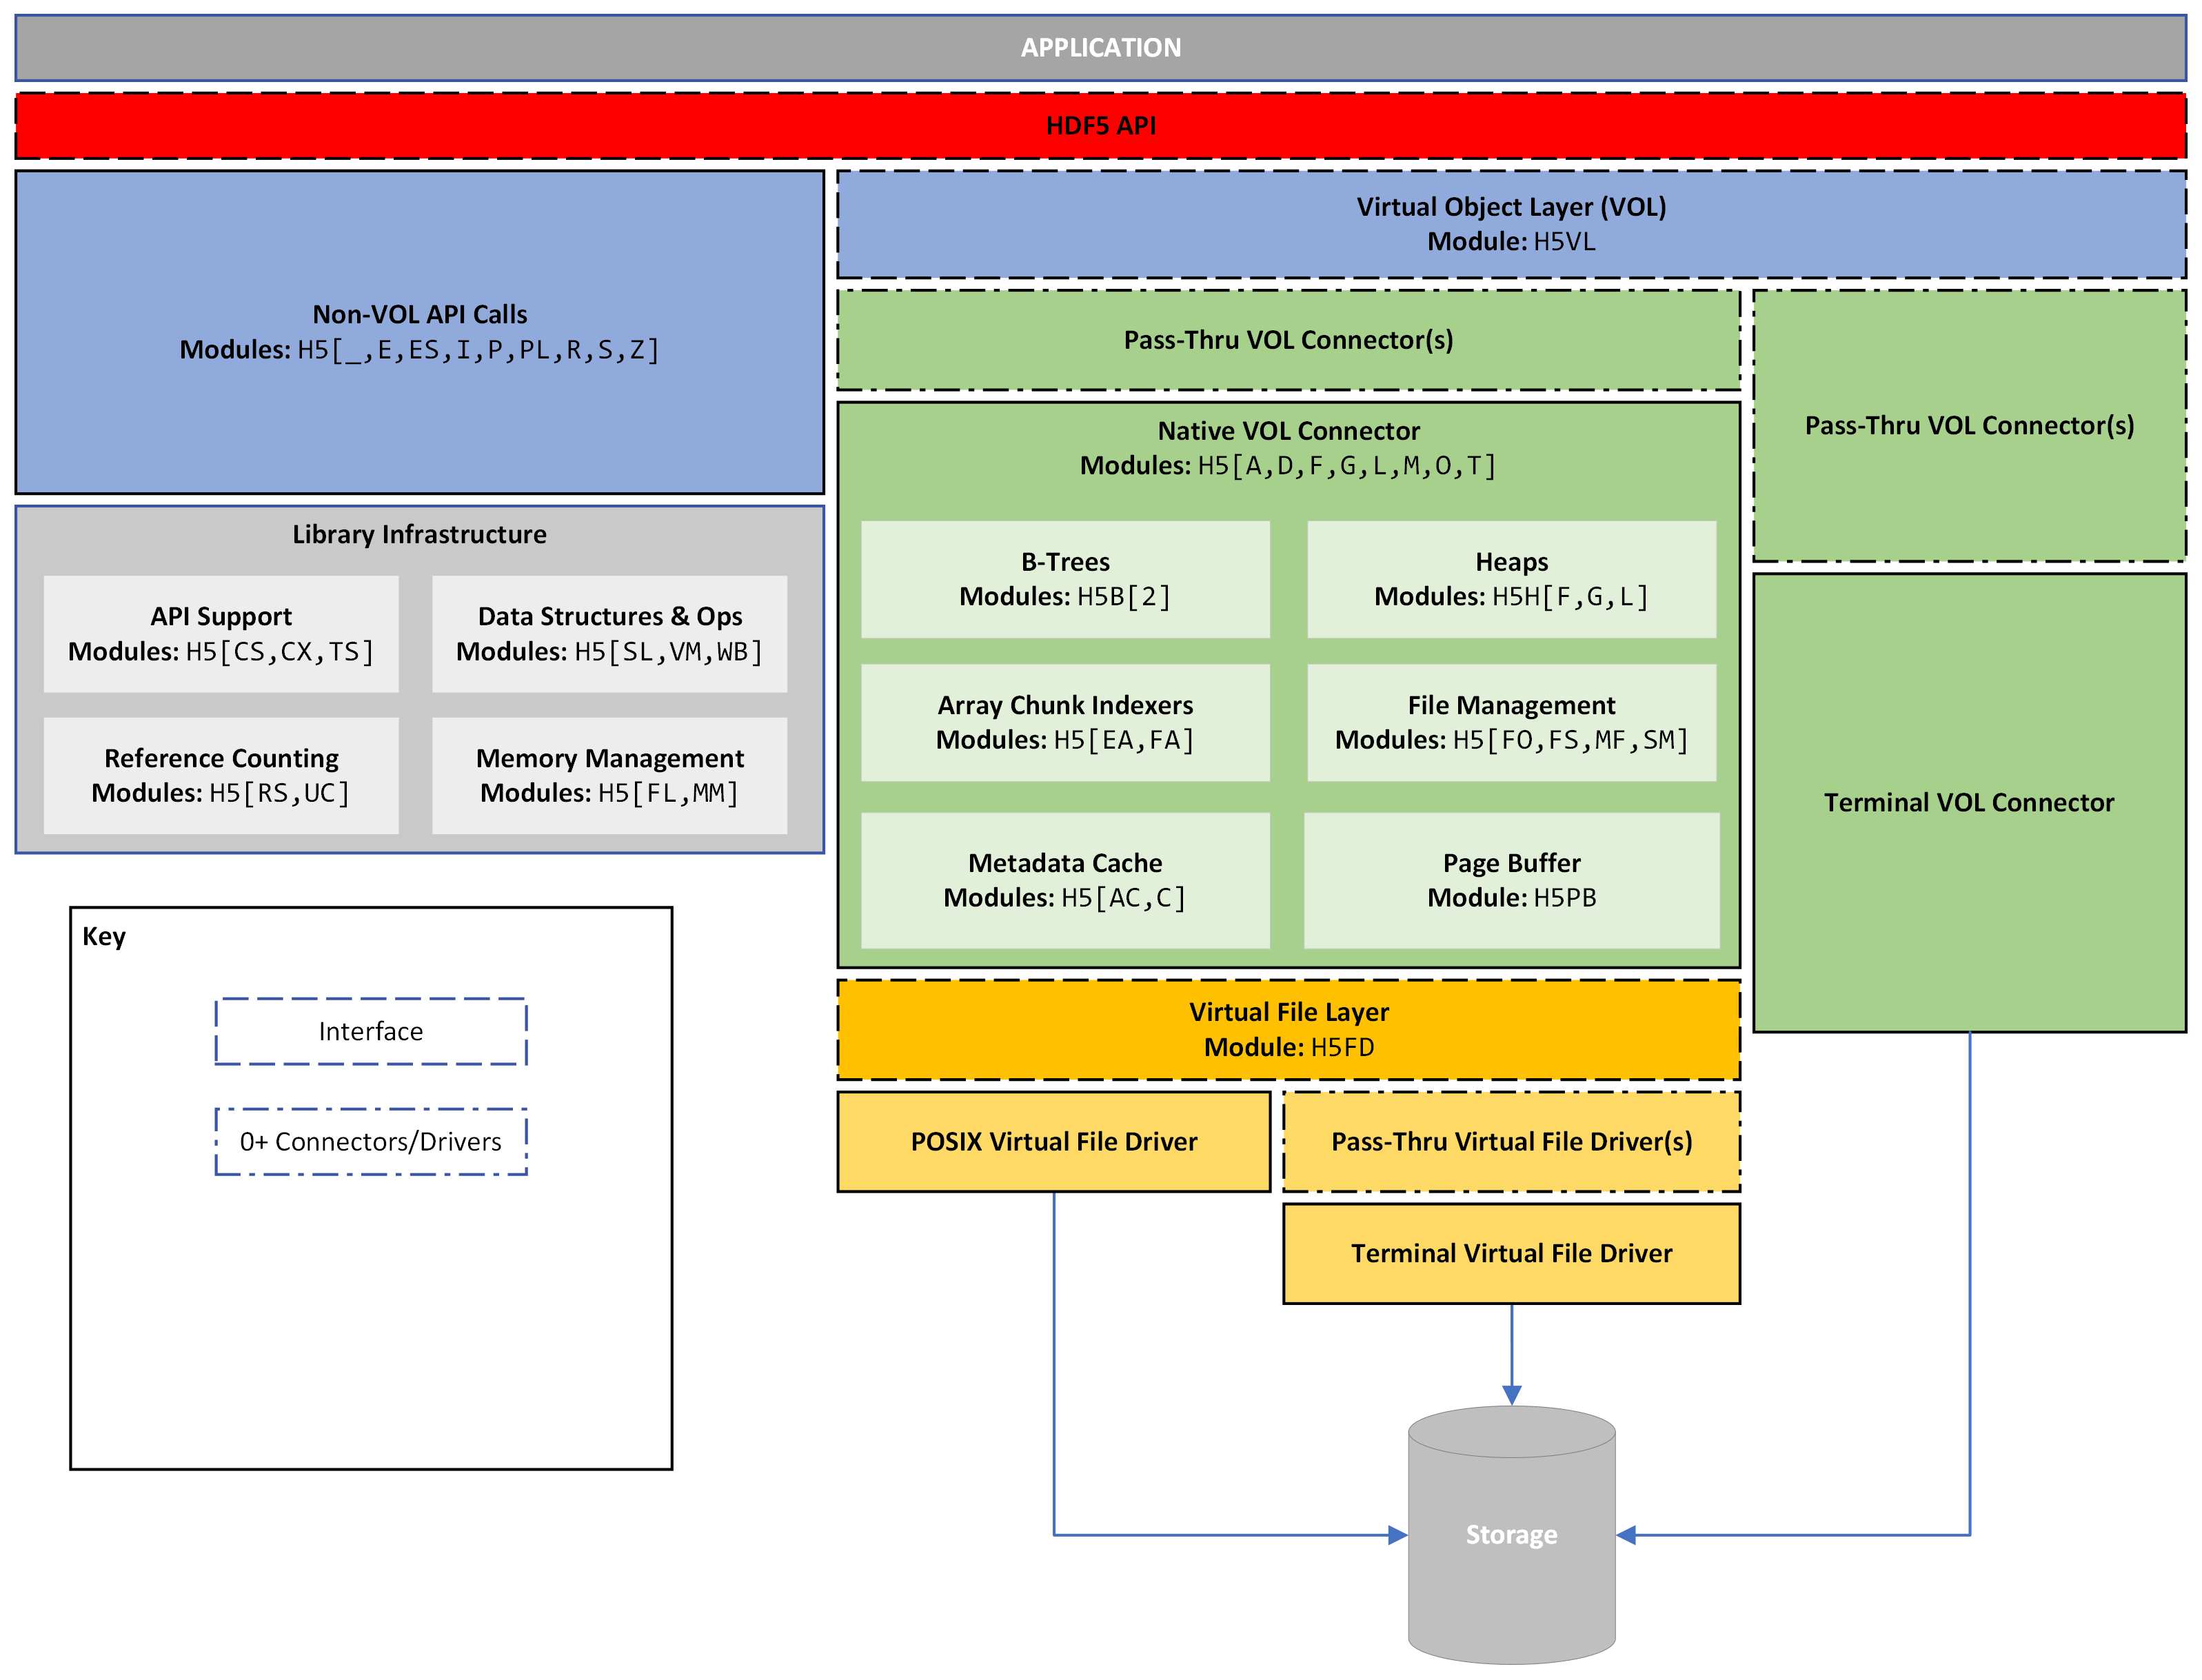
\includegraphics[scale=0.74,angle=90]{images/HDF5 library canvas.png}
\caption{The "location" of HDF5 library modules.\label{fig:module-location}}
\end{sidewaysfigure}
\end{landscape}

%\subsection{General Library Infrastructure (\texttt{H5})}
%\todo[inline]{Owner: ??? -- Priority: Low -- Effort: S}

\subsection{File Memory Allocation (\texttt{H5MF})}

%|  Name  | TODO | ONGOING | DONE |
%|--------|------|---------|------|
%| Dana   | x    |         |      |
%| Gerd   | x    |         |      |
%| Glenn  | x    |         |      |
%| Jordan | x    |         |      |
%| Luke   | x    |         |      |
%| Matt   |      |         |  x   |
%| Neil   | x    |         |      |
%| Scot   | x    |         |      |

%\todo[inline]{Owner: Matt -- Priority: Medium -- Effort: S -- Completion: 100\%}


The file memory management module \texttt{H5MF} is one of the major clients of the \Gls{fsm} module \texttt{H5FS}. Many file memory management routines act as wrappers around corresponding \Gls{fsm} operations. \texttt{H5MF} also manages some higher-level memory processes, such as paged aggregation (if enabled) and free space aggregators (if paged aggregation is disabled).

\begin{itemize}

    \item Allocation Types

\texttt{H5MF} uses the type of allocation requested to determine which type of \Gls{fsm} to create, open, or use for each file memory request. Allocation type indicates what type of low-level file element the allocated memory block is for. The allocation types are superblock, B-tree, raw data (\texttt{DRAW}), global heap, local heap, and object header. All of these allocation types besides 'raw data' are metadata.

    \item Free Space Aggregators

If the filespace management strategy is \texttt{H5F\_FSPACE\_STRATEGY\_FSM\_AGGR} or \\ \texttt{H5F\_FSPACE\_STRATEGY\_AGGR}, then small memory allocation requests are handled by two aggregators - one for raw data, and one for metadata. Aggregators are represented in memory with the \texttt{H5F\_blk\_aggr\_t} struct. Each aggregator maintains an 'allocation block' used to satisfy small memory requests of the appropriate type. These allocation blocks are allocated at the current \gls{eoa} and will be scattered more or less randomly throughout the file during normal operation. This scattered distribution can negatively impact performance and was a significant motivation for developing paged aggregation. If an aggregator does not have enough space in its current allocation block to satisfy an allocation request, the file is extended to satisfy the request. This extension also occurs whenever an allocation request exceeds the size of an allocation block.

    \item Paged Aggregation

If the filespace management strategy is \texttt{H5F\_FSPACE\_STRATEGY\_PAGE}, paged aggregation is enabled, and the raw data/metadata aggregators are disabled. They are replaced by a set of 'small' and 'large' \Glspl{fsm}. These \Glspl{fsm} group allocations into pages, making the aggregators unnecessary. The small \Glspl{fsm} track free sections which are smaller than the filespace page size, and attempt to satisfy small allocation requests. If a small \Gls{fsm} cannot satisfy an allocation, it requests additional memory from a large \Gls{fsm}. A large \Gls{fsm} tracks free sections that are equal to or larger than the filespace page size, and attempts to satisfy large allocation requests. If a large \Gls{fsm} cannot satisfy an allocation, it requests additional memory from the VFD.

For a file with a contiguous address space, the default behavior is to use two small \Glspl{fsm} (one for raw data and one for metadata) and one large \Gls{fsm} (for all large allocations, regardless of whether they are raw data or metadata). For a file with non-contiguous address space, it is possible to have up to 6 small \Glspl{fsm} and 6 large \Glspl{fsm}. These correspond to the six file space types: raw data and five types of metadata.

    \item Persistent Free Space Tracking and Self-Referential \glspl{fsm}

Filespace allocations and their associated \Glspl{fsm} can be divided into three categories: allocations and \Glspl{fsm} for raw data, allocations and \Glspl{fsm} for metadata other than \Glspl{fsm}, and allocations and \Glspl{fsm} which handle memory for \Glspl{fsm} themselves. This last category is called "self-referential \Glspl{fsm}". Non-self-referential \Glspl{fsm} are stored in the raw data \Gls{fsm} region of the metadata cache. It may seem confusing that some metadata \Glspl{fsm} are stored in a cache region named for raw data \Glspl{fsm}, but this is because they may be treated like raw data \Glspl{fsm} by the cache, while self-referential \Glspl{fsm} require special handling.

If persistent free space tracking is enabled, \Glspl{fsm} are written to the file. Before they are written to file, they must be 'settled' in order to minimize filespace used, remove redundant or outdated information from the file, and allow for self-referential \Glspl{fsm} to be written in a consistent and safe manner. Settling non-self-referential \Glspl{fsm} involves trimming the \gls{eoa}, deallocating filespace for old non-self-referential \Glspl{fsm} and the old \Gls{fsm} superblock extension message, and allocating new filespace for the current batch of non-self-referential \Glspl{fsm} and a new \Gls{fsm} superblock extension message. Non-empty (non-self-referential) \Glspl{fsm} are not written to the file, since they contain no useful information, and so no space is allocated for them. This settling process only involves deallocating and allocating memory, with all the actual data writes performed through the metadata cache later.

Self-referential \Glspl{fsm} must be settled after all non-self-referential \Glspl{fsm}. Self-referential-\Glspl{fsm} are settled in a slightly modified way to avoid two potential infinite loops. The first infinite loop would be allocating space for an \Gls{fsm} that is eventually found to contain no free space sections. This space would then need to be de-allocated again (because empty \Glspl{fsm} are not written to the file), potentially triggering an infinite loop. The second possible infinite loop would be allocating space for a free section info block and, in the process, increasing the size of that free section info block. This would necessitate reallocating that info block, potentially leading to an infinite loop. These loops are avoided by changing the settling process for self-referential \Glspl{fsm} in two ways. First, empty self-referential \Glspl{fsm} are written to file, unlike empty non-self-referential \Glspl{fsm}. Second, free section info blocks for self-referential \Glspl{fsm} are allowed to be oversized.

Settling self-referential \Glspl{fsm} requires saving the \gls{eoa} to file. Because the split and multi-file drivers work with multiple files, resulting in multiple valid \glspl{eoa}, persistent filespace management is not supported with those VFDs. 

\end{itemize}

\subsection{Free Lists (\texttt{H5FL})}

%|  Name  | TODO | ONGOING | DONE |
%|--------|------|---------|------|
%| Dana   | x    |         |      |
%| Gerd   | x    |         |      |
%| Glenn  | x    |         |      |
%| Jordan | x    |         |      |
%| Luke   | x    |         |      |
%| Matt   |      |         | x    |
%| Neil   | x    |         |      |
%| Scot   | x    |         |      |

%\todo[inline]{Owner: Matt -- Priority: Medium -- Effort: S -- Completion: 100\%}

The library's internal free lists module \texttt{H5FL}  is designed to allow the library to make as few calls to system memory functions as possible in order to improve performance. The primary interface exposed by this module to the rest of the library is a set of macros to define, add to, and remove free sections from a free list. Other modules in the library use these macros to create and operate on free lists associated with a particular struct in that client module. For example, the page buffer module uses a separate free list to handle memory for page buffers (\texttt{H5PB\_t}) and page buffer entries (\texttt{H5PB\_entry\_t}). These free lists, as an internal library optimization mechanism, are not tied to a particular file but to the library as a whole. The free list module sits below other modules that manage memory allocations at the file level, such as \texttt{H5FS} and \texttt{H5MF}.

Implementing the free list interface through macros allows for the free list operations to be silently replaced with system-free and allocate routines if free lists are disabled at build time. The option to disable free lists was implemented to simplify memory allocation debugging.

\begin{itemize}

\item In-memory objects

The library has four main types of free lists: 'regular' free lists for single internal data structures, array free lists for arrays of internal data structures, block free lists for arbitrarily sized blocks of bytes, and factory free lists for fixed-size blocks of bytes. Each of these free list types has its own set of structs used to represent it in the library. 

Each free list type has a head struct (\texttt{H5FL\_<type>\_head\_t}) that acts as the head of the free list. This head points to a list of free blocks that are all of the same fixed size. Each free list type has a node struct (\texttt{H5FL\_<type>\_node\_t}) that acts as the elements of the linked free list. 

% Block and array free lists make use of an additional structure \texttt{H5FL\_<type>\_list\_t} to store information about each individual block and array on the free list.

There is a fifth free list type, sequence free lists, that is a variation on array free lists. Sequence free lists are used to store free blocks for unbounded arrays of internal data structures. Sequence free lists are represented as a block free list with an additional field for sequence element size.

\item Block and Array Free Lists

Block and array free lists, due to supporting arbitrary size blocks of bytes, are slightly more complicated than other free list types. They are implemented using three architectural elements. The first element is lists of free blocks of a given size. Each element of this list is represented as an instance of \texttt{H5FL\_<type>\_list\_t}. Each element in the list stores information about each the free block/array. The second element is nodes, which sit either in a priority queue (for blocks) or in an array (for arrays). Each node is associated with a free list, and each node stores pointers to adjacent nodes. Nodes in the priority queue/array are represented as instances of \texttt{H5FL\_<type>\_node\_t}. The third element is a pointer to the head of the priority queue/array, represented by \texttt{H5FL\_<type>\_head\_t}. Figure~\ref{fig:block-free-list} shows the structure of a block free list.

\begin{comment} 
Figure drawing stored at https://thehdfgroup-my.sharepoint.com/:u:/g/personal/mlarson_hdfgroup_org/EY7BxMS5ll1DnLrxslw08q8BzyenrExg6KqG1PZ9HdUtpQ?e=4dNRHV
\end{comment}

\begin{figure}
    \centering
    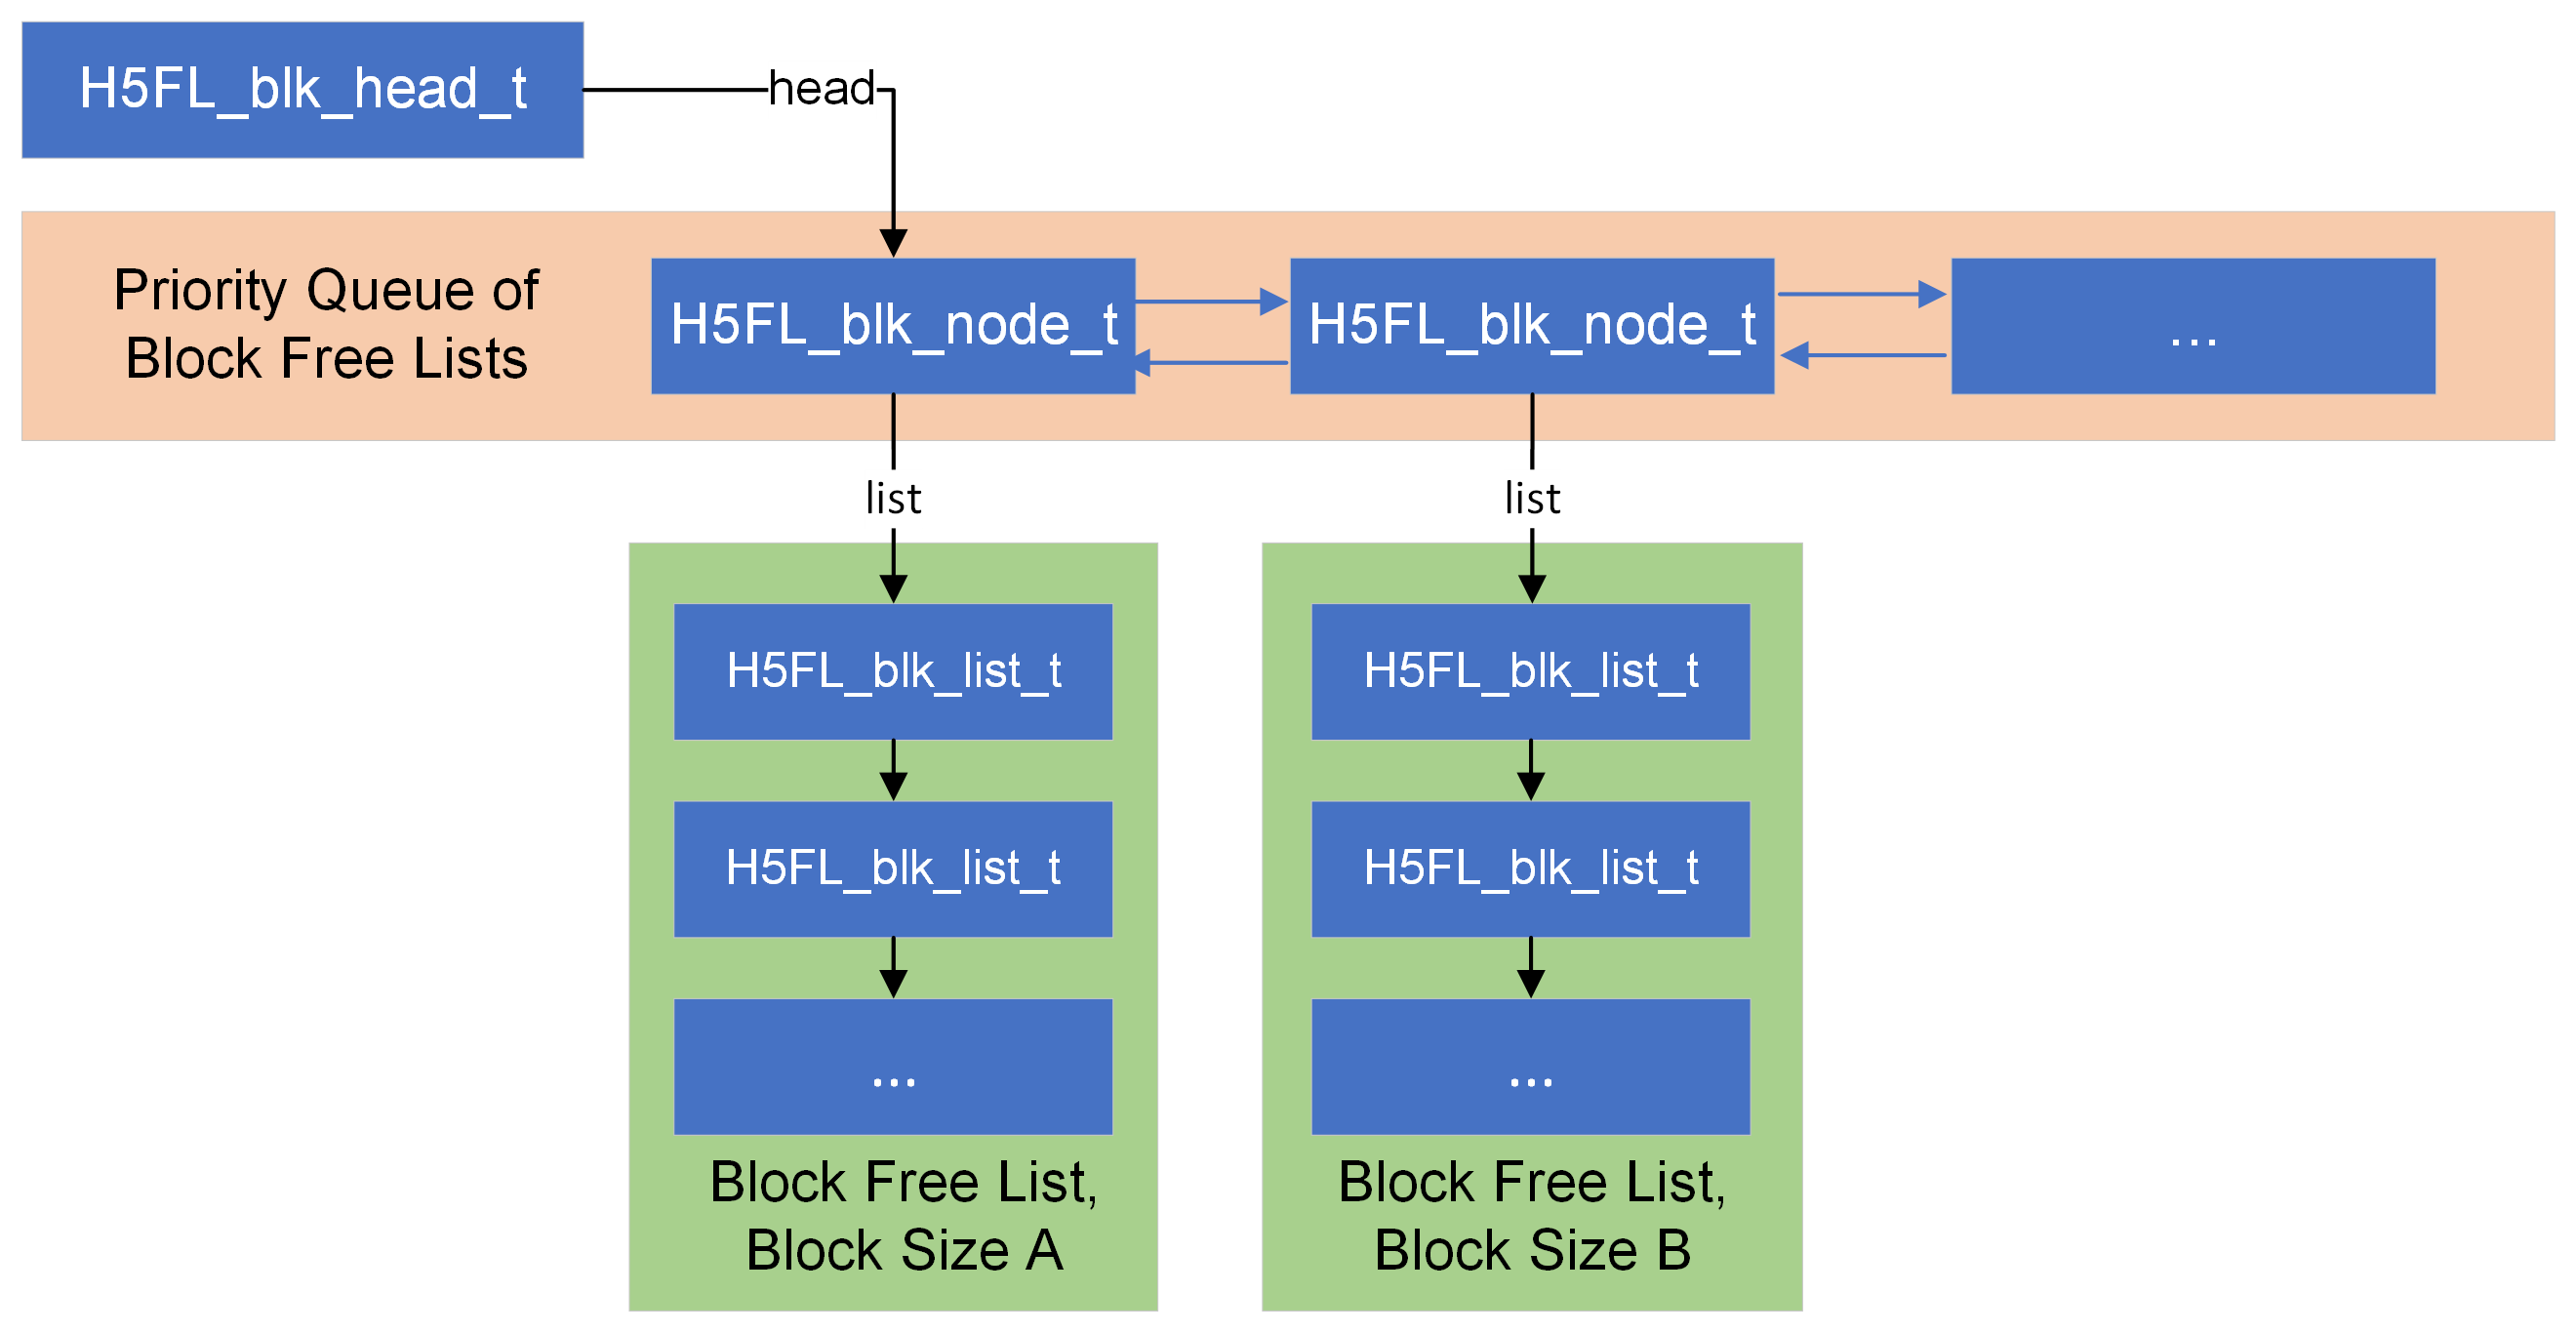
\includegraphics[width=0.8\textwidth]{images/block_free_list_diagram.png}
    \caption{A block free list}
    \label{fig:block-free-list}
\end{figure}

When a memory allocation for a block or array is requested from a free list, the collection of free lists for various block/array sizes is searched for the appropriate free list, and if a free list of the appropriate size is found, a block of memory from that free list is used. In the case of a free block list, the free list that was found is moved from its original position to the head of the queue, speeding up subsequent accesses.

\item Garbage Collection

A major benefit of library-handled free lists is that they enable library-handled garbage collection. Garbage collection is the process by which the library returns library-managed free space to the filesystem.

Garbage collection functionality is exposed to applications through \texttt{H5garbage\_collect}. This is one of many ways that the library exposes the memory and performance tradeoff to applications - less frequent garbage collection will use more memory but involve fewer system calls, while frequent garbage collection keeps memory overhead low but may involve slow allocations.

When a request for memory allocation (through \texttt{H5MM}) cannot be satisfied by the system, the library runs garbage collection and retries the system memory allocation call before throwing an error. This avoids a scenario where the library has memory available to it through free lists, but requests to the system for memory allocation fail due to the system being unaware of this memory.

\item Performance Considerations

Free lists are not created for all library types that require memory allocation. Because the free list infrastructure imposes some overhead in terms of memory and performance, only types that are expected to be allocated and deallocated many times during typical library operation are managed through a free list. Other types have their memory allocated and freed more directly through the \texttt{H5MM} module.

\end{itemize}

\subsection{API Contexts (\texttt{H5CX})}

%|  Name  | TODO | ONGOING | DONE |
%|--------|------|---------|------|
%| Dana   | x    |         |      |
%| Gerd   | x    |         |      |
%| Glenn  | x    |         |      |
%| Jordan | x    |         |      |
%| Luke   | x    |         |      |
%| Matt   |      |         |  x   |
%| Neil   | x    |         |      |
%| Scot   | x    |         |      |

%\todo[inline]{Owner: Matt -- Priority: Medium -- Effort: M -- Completion: 100\%}
\begin{itemize}

\item API Contexts vs. Global Variables

The primary goal of API contexts is to provide a way to get and set values from many different layers of the library during an API routine, without the performance penalty and complexity of extra parameters, and without the tight inter-module coupling and un-traceability of global variables.

To accomplish this goal, each API routine creates an API context containing fields. These fields control aspects of the operation, deciding things such as which VOL to use, or whether a metadata read is collective. Each of the fields in a context is associated with its own accessor ("get/set") routines. At the end of the API routine, the context is released. The temporary lifetime and accessor-based usage of API contexts avoid the shortcomings of global variables, while avoiding the performance penalty of passing around many extra parameters.

\item In-memory objects

An API context is represented by the \texttt{H5CX\_t} struct. This struct has at least one member for each field that is accessible through the API context interface. There are four distinct kinds of context fields, described in Table~\ref{table:H5CX_fields}

\begin{table}[h!]
\begin{tabular}{||c|m{0.70\textwidth}||}
\hline
\textbf{Context Field Type} & \textbf{Description} \\  [0.5ex] 
\hline\hline
Reference Property Lists &  The property lists to use for this operation. May be default or provided by the application. The context stores pointers to the underlying property list objects (\texttt{H5P\_genplist\_t}) without copying them. These fields are used to retrieve property lists for operations that require them in modules such as \texttt{H5FD}. \\
\hline
Internal Fields & Used for managing state that doesn't correspond to a property from a property list. Generally set at a high level and used at a low level. For example, the metadata "tag" is set in high-level group/dataset code and used in the low-level metadata cache. \\
\hline
Cached Fields &  Cached fields correspond to properties from property lists. In general, context fields are retrieved from the underlying property list and saved in the context on-demand. However, if the context contains a default property list, then the context fields are retrieved from cached fields instead. These cached fields are populated from the default property list during library initialization. These cached accesses are faster due to bypassing property list operations. Changes to cached field values do not propagate to the original property lists. \\
\hline
Return-Only Fields & Return-only fields correspond to properties from property lists that are never retrieved within the library and are only set with values in order to return those values to the application. When a value is set in a return-only field, that value is cached in the context until the context is destroyed when the API routine returns. At that time, any return-only fields that have changed have their new values written into the provided property list(s). \\
\hline
\end{tabular}
\caption{API Context Field Types}
\label{table:H5CX_fields}
\end{table}

Cached fields and return-only fields are paired with an additional field \texttt{<field\_name>\_valid}, used by macros that interact with that property. 

\item Reentrancy and The Context Stack 

Some API routines, such as \texttt{H5Literate}, involve user-defined callbacks which may themselves call API routines. Thus, API contexts must be re-entrant safe. This is handled by storing multiple API contexts on a stack, where the topmost context on the stack is used by the most recent API routine in the call stack.

Nodes on the API context stack are represented by the struct \texttt{H5CX\_node\_t}. Each node contains a pointer to an \texttt{H5CX\_t} instance with the actual information for that context, and a pointer to the next (lower) node in the stack. 

Each API call uses the macro \texttt{FUNC\_ENTER\_API} (or \texttt{FUNC\_ENTER\_API\_NOCLEAR}) to initialize and allocate a new context node. This context node is pushed to the top of the context stack by \texttt{H5CX\_push}. The end of each API call uses the macro \texttt{FUNC\_LEAVE\_API} to free the context node and remove it from the context stack with \texttt{H5CX\_pop}.

\texttt{H5CX\_push\_special}/\texttt{H5CX\_pop\_special} are only used in the library termination routine \\ \texttt{H5\_term\_library}. The normal push and pop routines use the library's free-list memory allocation and free routines. During library termination, the free-list and memory management structures are shut down. Thus, to avoid dependency on these structures, the special push and pop functions use system memory calls instead. 

\item API Context Setup

API routines need to use certain functions, depending on their parameters, to set up their API context correctly. The use case and description for each of these functions are in Table~\ref{table:H5CX_functions}.

\begin{table}[h!]
\begin{tabular}{||c|m{0.25\textwidth}|m{0.45\textwidth}||}
\hline
\textbf{Context Function} & \textbf{Use Case}  & \textbf{Description} \\  [0.5ex] 
\hline\hline
\texttt{H5CX\_set\_apl} & Routines with an access property list parameter & Stores the access property list in the context, sets the collective metadata read flag in the context, and enables sanity checks during collective API operations. \\
\hline
\texttt{H5CX\_set\_loc} & Routines that modify file metadata \textbf{without} an access list parameter & Sets the collective metadata read flag in the context, and enables sanity checks during collective API operations. \\
\hline
\texttt{H5CX\_set\_lapl} &  Routines which have both an object-specific access property list, and a link access property list (LAPL) & When a routine takes two access property lists, the object-specific access property list should be set with \texttt{H5CX\_set\_apl}, and the LAPL should be set with \texttt{H5CX\_set\_lapl}. \\
\hline
\texttt{H5CX\_set\_dxpl} &  Routines with a data access property list (DXPL) parameter & Stores the provided DXPL in the context. \\
\hline
\end{tabular}
\caption{API Context Setup Routines}
\label{table:H5CX_functions}
\end{table}

\item Thread Safety and Parallel

Each API context stack is thread-local. As a consequence, API contexts are inherently thread-safe, and API contexts do not require special consideration when using parallel HDF5. Several fields in the context are used to store and retrieve information about collective operations for the MPI-IO VFD, but this procedure is rank-local and entirely adheres to the usage pattern of other context fields.

\end{itemize}

\subsection{Error Handling (\texttt{H5E})}
\todo[inline]{Owner: Matt -- Priority: Low -- Effort: M - Completion: 100\%}

\begin{itemize}

\item Error Messages

An error message is an in-memory object represented by the \texttt{H5E\_msg\_t} struct. An error message contains a string describing the error that occurred, a 'type' indicating whether the error is major or minor, and a pointer to the error class it belongs to. Because error messages contain a dynamically allocated error string, they are reference-counted objects which are assigned handle IDs by the library, and have their own create and close API (\texttt{H5Ecreate\_msg}, \texttt{H5Eclose\_msg}).

\item Error Records

Error records are complete descriptions of individual errors. An error record is implemented as the \texttt{H5E\_error2\_t} struct, which consists of a major error message, a minor error message, an error class, a description of the specific error that occurred, and the location at which the error occurred in the source code. 

\item Error Stacks

An error stack is a collection of error records. By default, when an error occurs in a library function, an error record is pushed onto the active error stack and that function returns a failure indication. Its caller detects the failure, pushes another error record onto the stack, and returns another failure indication. This continues until the API function called by the application returns a failure indication. The library has a default error stack. Generally, errors cause this stack to be printed to the standard error stream automatically. \texttt{H5E\_DEFAULT} may be provided as an error stack ID to indicate the library's default error stack to error API functions. The library's currently active error stack is stored as the globally accessible \texttt{H5E\_stack\_g}. 

An error stack is implemented as an \texttt{H5E\_t} struct. Each error stack is created with space for a fixed amount error records. If more than this amount of errors are pushed onto a single stack, excess error records are truncated, and only the innermost errors will remain.

When an error record is pushed onto an error stack, the information of the record is not copied. Pointers to the record's error class and error messages are stored, and \texttt{H5I\_inc\_ref} increases the reference count of those objects. Correspondingly, when a record is removed from a stack, these pointers are removed and the reference count to the record's fields are decreased via \texttt{H5I\_dec\_ref}.

Most top-level API functions clear the active error stack upon entry, through the \texttt{FUNC\_ENTER\_API} macro, which calls \texttt{H5E\_clear\_stack}. Certain error-handling API functions, such as \texttt{H5Eprint2}, do not clear the error stack, since this would destroy the information they are meant to work with. Error clearing is avoided by replacing the API entry macro with the similar \texttt{FUNC\_ENTER\_API\_NOCLEAR}. Private library functions, which call \texttt{FUNC\_ENTER\_NOAPI} upon entry, and package library functions, which use \texttt{FUNC\_ENTER\_PACKAGE} upon entry, do not clear the error stack.

\item Error Reporting Macros

Error reporting in library functions is usually handled by the macro \texttt{FUNC\_GOTO\_ERROR}. This macro takes a major and minor error code, a return value to indicate failure, and a message. If automatic error reporting is enabled, it uses the preprocessor macros \texttt{\_\_FILE\_\_}, \texttt{\_\_func\_\_}, and \texttt{\_\_LINE\_\_} to add an error to the active error stack with information about the file, function, and line on which the error occurred. Afterwards, it jumps to the \texttt{done} label of the parent function, where cleanup and failure handling are generally performed.

If an error occurs after the \texttt{done} label, use of \texttt{FUNC\_GOTO\_ERROR} could potentially result in an infinite loop. To prevent this, the macro \texttt{FUNC\_DONE\_ERROR} performs the same error reporting without jumping to the \texttt{done} label, and is used whenever an error occurs during function cleanup or error handling.

\item Error Classes

 An error class is a collection of major and minor error messages. Error records must belong to an error class. An application can register a new custom error class with the library via \texttt{H5Eregister\_class}. An error class is implemented as a \texttt{H5E\_cls\_t} struct containing only the three strings provided to \texttt{H5Eregister\_class}, consisting of the error class's name, the library to which the error class belongs, and the version of that library. When using \texttt{H5Eprint2}, the error class of a set of records is displayed as \texttt{<ERROR\_CLASS>-DIAG}. 

\item Customized Error Handling

A user can define their own error reporting callback of type \texttt{H5E\_auto2\_t}. When an API function returns a failure indication, this callback will be invoked on the error stack. The default error reporting callback, \texttt{H5Eprint2}, uses \texttt{H5Ewalk} to traverse the individual error records within an error stack. \texttt{H5Ewalk} invokes a \texttt{H5E\_walk\_t} callback on each error record, and traverses the error stack.

\texttt{H5Eget\_current\_stack} registers the library's current error stack as an in-memory object, and assigns it a handle ID. This clears the active error stack, but leaves the error records that were in the active error stack accessible within the returned error stack object. Once an error stack is assigned a handle, custom error handling can be performed directly through the error API. 
\end{itemize}

% \subsection{Handles \& IDs (\texttt{H5I})}\label{ref:handles}
% \todo[inline]{Owner: ??? -- Priority: Medium -- Effort: M -- Completion: 0\%}

% Rough outline
% \begin{itemize}
%     \item What is an ID?
%         \begin{itemize}
%             \item A library-managed, reference-counted, handle
%             \item ID types
%             \item ID structure
%             \item Library vs. user-defined
%         \end{itemize}
%     \item ID management
%         \begin{itemize}
%             \item Storing and accessing IDs
%             \item Underlying data
%             \begin{itemize}
%                 \item VOL
%                 \item non-VOL
%                 \item Datatypes are a hybrid
%             \end{itemize}
%             \item Accessing the stored data
%             \item Reference counting
%         \end{itemize}
%     \item Example life cycle
%     \item Special considerations
%         \begin{itemize}
%             \item Initialization and shutdown of the H5I package
%             \item Global state and thread-safety considerations
%             \item Future IDs
%             \item Iterating and deletion
%             \item Flushing and ID preservation
%         \end{itemize}
% \end{itemize}

\subsection{Metadata Cache (\texttt{H5[AC,C]})}

%|  Name  | TODO | ONGOING | DONE |
%|--------|------|---------|------|
%| Dana   | x    |         |      |
%| Gerd   | x    |         |      |
%| Glenn  | x    |         |      |
%| Jordan | x    |         |      |
%| Luke   | x    |         |      |
%| Matt   |      |         |  x   |
%| Neil   | x    |         |      |
%| Scot   | x    |         |      |

\todo[inline]{Owner: Glenn -- Priority: High -- Effort: M -- Completion: 60\%}

The metadata cache is a cache meant for speeding up access to HDF5 metadata, and has support for features such as cache size adjustment under automatic or user program control. 

The cache itself is like a very modified version of the UNIX buffer cache, and uses a "Least Recently Used" (LRU) replacement policy to determine which items within the cache get evicted first. Due to the fact that the metadata written to a file can grow without bounds, the size of the metadata cache must reflect this ability, and no max entry amount can be set. Instead, users may set a maximum size, and eviction will occur as necessary using the LRU replacement policy. Similarly to UNIX, when dirty entries reach the end of the cache, they are flushed, marked as clean, and reset to the beginning of the cache. When running in parallel, only process 0 is allowed to write metadata to the file, and it does so only at synchronization points.

It is possible to tell when the size of the cache is a problem and must increase based on the hit rate, which is calculated over a period of time known as an epoch. When the hit rate has been low for a while, it means that the cache is probably at maximum capacity, and its capacity is probably not big enough. If this is the case, the size will increase according to some user-defined multiple. 

In addition, if the metadata entry is larger than the cache itself, this could also cause problems. This issue is fixed whenever it appears by taking the size of the metadata entry, multiplying it by some preset factor, and increasing the size of the cache based on this new size. 

Both of the above problems may arise when cache sizes are too big. Similarly, issues can occur when the cache size is too small. However, this is harder to judge. Ageout with hit rate threshold is the default cache size reduction algorithm of choice, and it combines two methods of detecting an oversized cache size. The first involves checking the hit rate once again. If the hit rate exceeds some preset amount, it might mean that the cache size is too big and needs to be reduced. Then, the second part of the algorithm, checking for metadata entries that haven't been accessed in some amount of epochs, kicks in and removes aged out entries. 

The metadata cache's configuration information is stored in a \texttt{H5AC\_cache\_config\_t} struct. This struct contains fields for general information, size increase control fields, size decrease control fields, and parallel configuration fields. 

\subsection{Files and the Open File List (\texttt{H5F})}

%|  Name  | TODO | ONGOING | DONE |
%|--------|------|---------|------|
%| Dana   | x    |         |      |
%| Gerd   | x    |         |      |
%| Glenn  | x    |         |      |
%| Jordan | x    |         |      |
%| Luke   | x    |         |      |
%| Matt   |      |         |  x   |
%| Neil   | x    |         |      |
%| Scot   | x    |         |      |

%\todo[inline]{Owner: Matt -- Priority: High -- Effort: L - Completion: 100\%}

\begin{itemize}
    \item File in-memory objects

Each successful \texttt{H5Fopen} results in a top-level file descriptor \texttt{H5F\_t}. By contrast, \texttt{H5F\_shared\_t}, the underlying structure storing information about the opened file, is allocated only once for each file in storage and is shared between file descriptors that point at the same file. Most of the fields in \texttt{H5F\_shared\_t} represent information related to persisting HDF5 files in a file system according to the file format specification~\cite{ffmt}. The shared file also tracks how many file descriptors point to it, and is only closed when its last file descriptor is closed.

The shared file contains a list of all opened objects, while each file descriptor maintains only counts of how many times each object is opened through that particular file descriptor. This division of information ensures that closing a file descriptor only decrements references that originated through that descriptor. For similar reasons, each file descriptor tracks the total number of objects it has open, excluding the root group.

Most information about child files mounted onto a parent file is kept in a table on the shared file structure of the parent file. The file descriptor maintains only a count of how many files were mounted through itself, similar to its count for open objects. The number of mounted files is maintained so that a file descriptor will close when 1. a weak close (see the section 'File open and close') was previously performed on it, and 2. an object is closed, and the only open objects remaining on the file descriptor are mounted groups. 

The shared file also contains information necessary for I/O, such as the file's permissions in storage, a page buffer, and any free space managers.

 \item Open file list

The file module maintains a list of open shared file objects, \texttt{H5F\_sfile\_head\_g}. Newly opened files are appended to the head of this list. This list is searched when checking if a file is already open. The actual comparison to determine if a potentially non-open file matches an open file is handled by the active VFD, which is not required to provide a way to compare files. If it does not provide such a method, then the application opening multiple handles to the same file will result in undefined behavior, and it is the responsibility of the application to ensure that the same file is not opened multiple times.

The open file list is implemented as a linked list. Due to the need to search this list upon each file open, performance may degrade if there is a large number of open files. The library is optimized for a small number of top-level files that contain many groups and objects in their internal file hierarchy.

    \item File open and close

File opening is first attempted without creating or truncating any files. This allows attempts to truncate or re-create currently opened files to safely fail without modifying any state. If the file is not already open, then the open proceeds normally, modifying files as requested, and the resulting shared file object is added to the open file list.

Each FAPL has a 'file close degree' which determines how open objects within a file are handled at file close. The 'weak' close degree allows the file handle to be closed from the application's perspective (as tracked by the \texttt{closed} flag on a file descriptor), but keeps the file handle around until all objects under it are closed. The root group and the root groups of any mounted files are not considered open objects for this purpose, and a weak close will be completed if such groups are the only open objects remaining. The 'semi' close degree causes a file close to fail if any objects remain open. The 'strong' close degree causes any open objects to be closed before the close completes. Most VFDs default to 'weak', except for the MPI-I/O driver which defaults to 'semi', due to file closes being a collective operation. When HDF5 files are mounted, the parent and child files must have the same close degree in order to avoid contradictions in how to handle objects at close time.

Closing an object may or may not evict it from the file's metadata cache, depending on the 'evict on close' setting. This setting trades increased memory with a larger cache for higher speed, or lower speed with a smaller cache for decreased memory usage.

    \item External file cache

The external file cache (EFC) is a mechanism for keeping files opened through external links quickly accessible for subsequent accesses. Each shared file structure may have an EFC that stores information about files accessed through external links in that shared file.

EFC entries are linked to the top-level file descriptor, as the EFC caches the result of opening an external file (a top-level file descriptor). Because file descriptors are not reference counted, EFC entries must be reference counted within the EFC in order to handle dependencies in the EFC tree.

A file's EFC contains both a skip list of cache entries and the head of a cache entry list sorted by the least recent update (LRU) time. The skip list is used to check whether a newly opened external file is already present in the cache. The LRU-sorted list speeds up the common case of closing the most recently opened external file and allows the least-recently accessed cache entry to be dropped when the maximum size of the EFC is reached.

\end{itemize}

% \subsection{File Space Management and Free Space Tracking (\texttt{H5FS})}
% \todo[inline]{Owner: ??? -- Priority: Medium -- Effort: M -- Completion: 0\%}

\subsection{File Page Buffer (\texttt{H5PB})}\label{sec:H5PB}

%|  Name  | TODO | ONGOING | DONE |
%|--------|------|---------|------|
%| Dana   | x    |         |      |
%| Gerd   | x    |         |      |
%| Glenn  | x    |         |      |
%| Jordan | x    |         |      |
%| Luke   | x    |         |      |
%| Matt   |      |         |   x  |
%| Neil   | x    |         |      |
%| Scot   | x    |         |      |

%\todo[inline]{Owner: Matt -- Priority: High -- Effort: M -- Completion: 100\%}

The page buffer exists within the native VOL, just above the VFL and just below the I/O layer. Thus, the library can benefit from the page buffer cache regardless of which VFD is active. 

There are a few conditions under which file I/O bypasses the page buffer entirely: if page buffering is disabled, if the requested I/O operation is larger than one page and thus would not benefit from the page buffer, or if the requested operation is a parallel raw data access. Additionally, when opening a file with page buffering enabled, the superblock contains information needed to initialize the page buffer (e.g. page size). Because this information must be read from the superblock before the page buffer is initialized, the page buffer cannot be used for this operation.

The page buffer's page size will be rounded down to the nearest multiple of the file space page size, in order to avoid situations where reading or writing in blocks of page size could extend outside the bounds of the file.

\begin{itemize}

    \item In-memory objects

A page buffer is represented in memory by the struct \texttt{H5PB\_t}, which is attached to a shared file object. Page buffers are associated with the shared file so that different handles to the same file share the same page buffer.

The page buffer maintains three lists of pages. The first is a skip list of page entries allocated by the page buffer itself. The second is another skip list containing only the page entries inserted by the free space manager. The free space manager inserts blank pages into this list during reads of file regions that have never been written to, in order to avoid unnecessary file accesses. The third list is a linked list of page entries sorted by the least recent update (LRU). The LRU-sorted list is used to evict the oldest page entries when the maximum size of the page buffer is reached. 

Page buffer entries (\texttt{H5PB\_entry\_t}) consist of their location in the file, pointers used to maintain the LRU-list, and an indication of whether the page buffer entry contains metadata or raw data. 

    \item Metadata vs Raw Data

I/O operations accessing a metadata entry are always atomic - the entire entry is always accessed. Noncontiguous subsets of raw data may be accessed using selections, and so I/O operations on raw data through the page buffer require some additional steps. During raw data writes, the page buffer needs to update any pages that are partially modified by large (greater than page size) writes, and discard any pages that are entirely overwritten. Similarly, during raw data reads, the page buffer must collect data from any dirty pages that are within the span of the I/O request. 

The utility of storing metadata versus raw data in the cache will vary from use case to use case. To allow applications to optimize for their particular case, and to avoid a scenario where one type of data is completely evicted from the page buffer cache, applications may set a minimum percentage of the page buffer's memory to be reserved for each type of data.

A page in the page buffer must contain only metadata or only raw data. This restriction is imposed in order to properly map pages to regions of the file in storage, as metadata and raw data are not interleaved within pages in storage (with the default driver).

    \item Page Buffering in Parallel

Parallel HDF5 has limited support for the page buffer due to the need for all processes to have a mutually consistent view of the data.

Because all operations that modify metadata must be performed collectively, the page buffer can be used during parallel metadata I/O if the metadata write strategy has a single process handle all writing of dirty metadata from cache. This is accomplished by having the writer-process write all dirty entries to the page buffer, flush the page buffer to storage, and then update the other ranks with the metadata entries that were written.

The page buffer is always bypassed when reading or writing raw data in parallel. When accessing raw data collectively, the HDF5 library constructs MPI-derived datatypes to represent possibly non-contiguous buffers in memory and file offsets. At the page buffer layer, it would be necessary to flatten the derived datatypes, update the page buffers, and then impose additional communication among all processes to determine who reads/writes which pages for the collective operation. This would represent considerable overhead and complexity, and replicate work that is more logically handled by MPI itself. Simply bypassing the page buffer likely leads to better performance than this implementation would. Additionally, most parallel raw data accesses are large enough that the page buffer would not provide a significant benefit. While many of these issues would not apply to parallel independent raw data access, concurrent use of collective and independent operations would cause the page buffers of the processes involved in each operation to become inconsistent with one another, and thus the page buffer is bypassed during all parallel operations regardless of whether they are collective or independent.

When using Single Writer Multiple Reader (SWMR), the writer may not make use of a page buffer. The SWMR writer has a required order for its operations, which would not be preserved by the page buffer. SWMR readers can use the page buffer with only one caveat. After a refresh operation is performed on an object, entries that get evicted from the metadata cache must have their corresponding pages evicted from the page buffer in order to avoid subsequent reads returning old data. 

\end{itemize}

\begin{comment}
\subsection{Virtual File Layer (\texttt{H5FD})}\label{ref:vfl}

%|  Name  | TODO | ONGOING | DONE |
%|--------|------|---------|------|
%| Dana   | x    |         |      |
%| Gerd   | x    |         |      |
%| Glenn  | x    |         |      |
%| Jordan | x    |         |      |
%| Luke   | x    |         |      |
%| Matt   | x    |         |      |
%| Neil   | x    |         |      |
%| Scot   | x    |         |      |

\todo[inline]{Owner: Luke -- Priority: Medium -- Effort: S -- Completion: 0\%}

The Virtual File Layer (VFL) provides the ability to extend the native VOL to support I/O to different I/O backends. The purpose of the VFL is to decouple the file I/O functionality from the core HDF5 library, allowing for greater flexibility in supporting different storage mechanisms and file systems. It serves as a "plug-in" layer that allows HDF5 to work with various storage backends.



% \subsection{On-Disk Indexes (\texttt{H5[B,B2,EA,FA]})}
% \todo[inline]{Owner: ??? -- Priority: Low -- Effort: M}

% \begin{itemize}
%     \item v1 B-trees
%     \item v2 B-trees
%     \item Fixed arrays
%     \item Extensible arrays
% \end{itemize}

% \subsection{On-Disk Heaps (\texttt{H5H[F,G,L]})}
% \todo[inline]{Owner: ??? -- Priority: Low -- Effort: M}

% \begin{itemize}
%     \item Local heaps
%     \item Global heaps
%     \item Fractal heaps
% \end{itemize}
\end{comment}

\subsection{File Objects (\texttt{H5[O,SM]})}

%|  Name  | TODO | ONGOING | DONE |
%|--------|------|---------|------|
%| Dana   | x    |         |      |
%| Gerd   | x    |         |      |
%| Glenn  | x    |         |      |
%| Jordan | x    |         |      |
%| Luke   | x    |         |      |
%| Matt   |      |         |   x  |
%| Neil   | x    |         |      |
%| Scot   | x    |         |      |

\todo[inline]{Owner: Neil -- Priority: High -- Effort: L -- Completion: 30\%}

File objects are the heart of the HDF5 data model. In the library, the object package (\texttt{H5O}) consists of structures and code common to all object types, as we use code to handle object headers, which are the central on-disk objects for storing HDF5 file objects. All objects contain an object header, which contains some fixed metadata and a variable list of object header messages, as well as any data referenced by those object header messages.

\begin{itemize}
    \item In-memory objects

The central in-memory structure for an object is \texttt{H5O\_t}, which is defined in \texttt{H5Opkg.h}. This structure essentially contains the information that is stored in the object header, including the list of object header messages. While it might seem natural for the type-specific object structs (such as \texttt{H5D\_t} for datasets) to contain an \texttt{H5O\_t} at the top (beginning) of the struct, this is not the case. \texttt{H5O\_t} is essentially a lower-level proxy for the object header on disk, while the type specific structures are closely tied to the logical objects exposed through the API.

One potential point of confusion is the \texttt{rc} field in the \texttt{H5O\_t} struct is not the same as the \texttt{rc} field in the struct returned by \texttt{H5Oget\_info()}. The \texttt{rc} in \texttt{H5O\_t} is the in-memory reference count of the memory struct itself, while the \texttt{rc} returned by \texttt{H5Oget\_info()} is the number of links to the object header in the file. The \texttt{nlinks} field in \texttt{H5O\_t} is equivalent to the link-counting \texttt{rc} from \texttt{H5Oget\_info()}.

    \item Object headers

The object header is the root piece of metadata for all HDF5 objects on disk. The object header consists of the main object header block, which in turn consists of the prefix containing generic object metadata, as well as some number of object header messages. If the number of messages grows too large to fit into the main object header block, one or more object header continuation chunks will be created on disk, each containing more object header messages. Object header continuation blocks are pointed to from their parent object header using an object header continuation message.

Since an object header is not a single block on disk, but is treated as a single object by most of the library, the way the metadata cache handles it is slightly strange. There are metadata cache clients for object header root blocks and continuation blocks, each of which serializes and deserializes these objects as needed. However, when the entire object header is retrieved, typically using \texttt{H5O\_protect()} or \texttt{H5O\_pin()}, which take an \texttt{H5O\_loc\_t} object location, these functions use the metadata cache to decode all the constituent blocks of the object header, protects (and optionally pins) the root object header block, then assembles and returns an \texttt{H5O\_t}. The \texttt{H5O\_loc\_t} struct is how other packages generally keep track of their objects and mostly consists only of a file and address of the root object header block.

    \item Object header messages

Object header messages encode the majority of the important metadata of the object. There are several different types of object header messages, and only some of them are present in any one object header. The type of an object is determined by which object header messages are present. For example, if a layout message is present, then the object is a dataset. Object header messages also appear in the file superblock, even though that is not an object header.

Each object header message type is defined in a separate source file, for example, \texttt{H5Olayout.c} for layout messages. Each message type defines itself using the \texttt{H5O\_msg\_class\_t} struct, which contains callback functions that must be implemented (some are optional) and other basic information about the message type. Most object header message types can only be present once in an object header, but there are some exceptions, such as attributes, link messages, and object header continuation messages. This distinction is important since \texttt{H5O\_msg\_read()} only reads the first message of a given type, so if there may be more than one message of that type, \texttt{H5O\_msg\_iterate()} must be used instead, with the callback operation checking to see if it is the correct message. The generic (type agnostic) object header message code stores messages in the \texttt{H5O\_mesg\_t} struct. This struct contains information on allocation within the object header, as well as pointers to the serialized/on-disk form (\texttt{raw}) and the deserialized/in-memory form (\texttt{native}). The in-memory structs for all the different message types are defined in \texttt{H5Oprivate.h}. They are defined in the private header because other packages widely use the native forms of these messages. This makes \texttt{H5Oprivate.h} one of the most important header files in HDF5, and can be thought of as a significant contributor to the coupling between the packages.

Allocation of space for object header messages is somewhat complicated and handled in \texttt{H5Oalloc.c}. This code handles allocation, deletion, free space tracking (with null messages), and the creation of new continuation blocks (in conjunction with the metadata cache and standard file space allocation code). This code needs to handle several corner cases, such as when a message is added when there isn't enough space for a continuation message (in this case it must move messages), or if there's empty space but there isn't space for a null message (in this case it encodes a "gap" value in the object header).

    \item Shared object header messages

To save space, the HDF5 library can optionally automatically check if object header messages are the same between different objects, and only store this message once if that is the case. Such messages are called shared object header messages, and can be stored either in one object's object header, or in the file's shared object header message heap. Additionally, these shared messages can be indexed either with a simple list or a v2 b-tree. Using a v2 b-tree obviously improves the performance of checking to see if a message is already shared, but requires a more recent file format version.

Object header messages that can be shared need to follow special steps in their definition files. First, they need to \texttt{\#include H5Oshared.h}, then, for the callbacks which are defined in \texttt{H5Oshared.h}, they need to \texttt{\#define} the callback from \texttt{H5Oshared.h} to a name specific to the message type (this name isn't actually defined in the message file, it's used to point to the shared function from the header), then do the same with the symbol that ends in \texttt{\_REAL}, defining it to be the name of the actual function implemented in the object header message definition file. For example, \texttt{H5Odtype.c} uses: \texttt{\#define H5O\_SHARED\_DECODE H5O\_\_dtype\_shared\_decode}, where \texttt{H5O\_\_dtype\_shared\_decode} is only used as the name for the \texttt{decode} callback in the \texttt{H5O\_msg\_class\_t} struct; \texttt{\#define H5O\_SHARED\_DECODE\_REAL H5O\_\_dtype\_decode}, where \texttt{H5O\_\_dtype\_decode()} is defined as the actual datatype decoding function in \texttt{H5Odtype.c}, which does not handle shared messages. Therefore, when the library decodes a datatype message, the code flows into \texttt{H5O\_SHARED\_DECODE()}, which locates the actual datatype message and then invokes \texttt{H5O\_\_dtype\_decode()} to do the actual decoding.

For callbacks that are not implemented by the object header message definition file, they must still \texttt{\#define} the callback from \texttt{H5Oshared.h} to a name and include that name in the class struct, but they may then \texttt{\#undef} the \texttt{\_REAL} version of the callback. In addition, the object header message definition file must \texttt{\#define H5O\_SHARED\_TYPE} to the name of the global variable containing its \texttt{H5O\_msg\_class\_t} class struct.

Additional code for handling shared messages in these callbacks is defined in \texttt{H5Oshared.c}, while most of the code for handling shared messages (allocation, search, etc.) is contained in the \texttt{SM} package. Code for handling the message in the file superblock which points to the shared message heap is contained in \texttt{H5Oshmesg.c}.

    %\item Object copying

%\todo[inline]{Object copying}

\end{itemize}

\subsection{Attributes (\texttt{H5A})}

%|  Name  | TODO | ONGOING | DONE |
%|--------|------|---------|------|
%| Dana   | x    |         |      |
%| Gerd   | x    |         |      |
%| Glenn  | x    |         |      |
%| Jordan | x    |         |      |
%| Luke   | x    |         |      |
%| Matt   |      |         |  x   |
%| Neil   | x    |         |      |
%| Scot   | x    |         |      |

%\todo[inline]{Owner: Matt -- Priority: High -- Effort: M -- Completion: 100\%}

\begin{itemize}
    \item Attribute in-memory objects

Attribute in-memory objects are represented with the \texttt{H5A\_t} structure, defined in \texttt{H5Apkg.h}. This structure contains information about whether the attribute is shared between multiple objects, the location of the attribute's parent object on disk, and the path to the attribute in the file hierarchy. The underlying shared attribute object \texttt{H5A\_shared\_t} contains information such as the size of the attribute, its dataspace and datatype, and its name. The shared \texttt{nrefs} field tracks the number of remaining references to the attribute from other objects in the file, and the attribute's resources are freed once this count is decremented to zero. 

The \texttt{crt\_idx} field tracks the creation index of the attribute, if creation index tracking is enabled on the parent object. This index only tracks the order in which attributes were created relative to each other, not any absolute information about the time of their creation.

    \item Compact and Dense Attribute Storage

There are two kinds of attribute storage: compact and dense. Compact attributes are kept in the object header of the parent object, along with other metadata for that object. Dense attributes are kept in a fractal heap. The address of the fractal heap for dense attribute storage is kept in the Attribute Info message in the object header. The heap IDs to access specific dense attributes in the fractal heap are stored in a name-index B-tree. 

If the file access property list used for a file is set for file format compatibility with library versions before 1.8 (as is the case by default), all attributes will be stored compactly, and the creation of attributes larger than 64 KiB will not be allowed.

The architecture for attribute storage is nearly identical to the architecture for link storage.

    \item Attribute object header messages (open/flush)

The primary fields that define an attribute are its datatype, dataspace, name, and the data it contains. When an attribute is compact, all of these fields are stored in an attribute object header message and inserted into the object header of the parent object. In library file format versions 1.6 and later, the datatype/dataspace fields in an attribute message may be pointers to a datatype or dataspace message that is shared between objects.

If an object is using dense attribute storage, then the object header will contain an attribute info message with the location of a name-index B-tree, as well as the address of the fractal heap storing the attribute messages.

Changes to object headers make use of caching for optimization. Attribute messages may be flushed to storage by use of \texttt{H5Fflush} on the containing file, or \texttt{H5(D/G/T/O)flush} on an object of the appropriate type with attached attributes. Note that these functions only directly control the library's buffers, not any buffering performed by the operating system. Flushing of object headers is also performed automatically by the library during certain operations.

    \item Attribute I/O

Attributes do not support partial reads or writes using selections. Any read or write to an attribute will operate on the attribute's entire dataspace. Attributes also do not support compression or chunking. Because attributes are intended to hold small quantities of metadata, these aspects of the I/O pipeline were omitted in order to optimize and simplify attribute I/O. If any of these I/O features are desired for use with metadata, then that metadata may be stored in a dataset instead, and a pointer to that dataset stored in an attribute - see the section "Dataset Storage Layouts".

Reads and writes to attributes use the same datatype conversion pipeline as read and writes to datasets.

If an attribute in compact storage is written to, all of its previous data in the object header is overwritten by an in-memory buffer that is later flushed to storage. If an attribute in dense storage is written to, a write operation is performed on the fractal heap at the heap ID storing the attribute by name. 

    \item Attribute iteration

The iteration process varies between compact and dense attributes.

Dense attribute iteration is handled by \texttt{H5A\_\_dense\_iterate}. If the iteration order was specified to be \texttt{H5\_ITER\_NATIVE} in order to optimize for speed, then the order is determined by the hashes of the attribute names in the name index B-tree. Otherwise, a table of attributes is built by \texttt{H5A\_\_dense\_build\_table}, sorted in the desired order by \texttt{H5A\_\_attr\_sort\_table}, and then iterated through by \texttt{H5A\_\_attr\_iterate\_table}.

The compact iteration case is similar: \texttt{H5A\_\_compact\_build\_table} creates a table of attributes, and iterates through it via \texttt{H5A\_\_attr\_iterate\_table}. For compact attributes, the table is always constructed, even when the iteration order is \texttt{H5\_ITER\_NATIVE}. 

The attribute table itself is the same, regardless of the storage type its attributes were retrieved from.

The architecture for attribute iteration is nearly identical to the architecture for link iteration. As with all forms of iteration in the library, attributes should not be created or removed during iteration - changes to the parent object's attribute count during iteration can lead to undefined behavior.

\end{itemize}

\subsection{Groups and Links (\texttt{H5[G,L]})}

%|  Name  | TODO | ONGOING | DONE |
%|--------|------|---------|------|
%| Dana   | x    |         |      |
%| Gerd   | x    |         |      |
%| Glenn  | x    |         |      |
%| Jordan | x    |         |      |
%| Luke   | x    |         |      |
%| Matt   |      |         |  x   |
%| Neil   | x    |         |      |
%| Scot   | x    |         |      |

%\todo[inline]{Owner: Matt -- Priority: High -- Effort: L -- Completion: 100\%}

A group is a potentially empty collection of link objects. The name of an object within a group is actually the name of a link that refers to it. The same underlying object may be referred to by multiple names, if it is pointed to by multiple links in one or more groups. When an object is created by a user, the library automatically creates a new hard link from the parent group to that object.

\begin{itemize}

    \item Group in-memory objects

Groups are represented by the \texttt{H5G\_t} struct. This struct has three elements: the location of the group within the file hierarchy as an \texttt{H5G\_name\_t} instance, the group's address within the file as an \texttt{H5O\_loc\_t} instance, and shared information for the group as an \texttt{H5G\_shared\_t} instance. The shared group information is available to all in-memory objects which refer to the same underlying group in the file, and allows a shared count of how many in-memory objects reference that particular group to be maintained. % This count is used to manage when the metadata cache is flushed. The metadata cache is flushed when the number of group in-memory objects for a particular group drops to zero (i.e. the last reference to that group is closed).

    \item Link storage

There are two kinds of link storage: compact and dense. Compactly stored links are kept in the object header for the group containing them, along with other metadata for that group object. Densely stored links are kept in a fractal heap. The address of the dense link fractal heap is then stored in the Link Info message in the group's header, with the heap IDs to access specific dense links stored in the name index B-tree. 

If the file access property list used for a file is set for file format compatibility with library versions before 1.8 (as is the case by default), all links will be stored in the file's symbol table.

% If compact storage is used, the link message is inserted into the header of the target group by \texttt{H5G\_\_compact\_insert}. The object header is pinned while the new message is appended, preventing it from being flushed to file, and unpinned after the operation is finished. When a compact link is accessed by name, the search is performed by \texttt{H5G\_\_compact\_lookup}, which iterates over the messages in the group header with \texttt{H5O\_msg\_iterate} and uses \texttt{H5G\_\_compact\_lookup\_cb} to check for a match by link name and copy the message if a match was found.

% If dense storage is used, the insertion of of the link is handled by \texttt{H5G\_\_dense\_insert}, which in turn uses \texttt{H5HF\_insert} to insert link information into the dense link fractal heap and \texttt{H5B2\_insert} to insert the link's name (and potentially, its creation order) into a v2 B-tree. Accessing dense links is handled by \texttt{H5G\_\_dense\_lookup}, which uses \texttt{H5B2\_find} to search the name index v2 B-tree for a dense link with the target name. If the dense link is found, then the provided callback \texttt{H5G\_\_dense\_lookup\_cb} copies the link message information.

The architecture for dense/compact link storage is nearly identical to the architecture for attribute storage.

    \item User-defined links

Users may register a user-defined link class with \texttt{H5Lregister}, and then create a link of that class using \texttt{H5Lcreate\_ud}. A link class definition must at minimum include a version number for the link class struct \texttt{H5L\_class\_t}, a link class identifier \texttt{class\_id}, and a traversal function \texttt{trav\_func}. \texttt{link\_class} must be in the range between \texttt{H5L\_TYPE\_UD\_MIN} and \texttt{H5L\_TYPE\_UD\_MAX}. Note that external links are implemented as an example of a user-defined link class, using \texttt{class\_id} = \texttt{H5L\_TYPE\_UD\_MIN}.

User-defined link classes may also provide optional callback functions to create, move, copy, delete, and query an instance of the link class. Some functionality is automatically implemented for these callbacks as a consequence of the type-independent link architecture. 

Depending on the user's implementation of the link callbacks, user-defined links may or may not affect the \texttt{nlinks} count of objects, and may or may not be allowed to dangle.

    \item Link traversal

"Link traversal" refers to the process of following links to their target objects. When opening an object through a link, the link's target location in the file hierarchy is iteratively determined by \texttt{H5G\_traverse}, and once the target location is reached, location information specifying position within the file hierarchy (\texttt{H5G\_name\_t}) and within the file (\texttt{H5O\_loc\_t}) is copied to the opened object.

For hard links, if the hard link points to a mounted file, then \texttt{H5F\_traverse\_mount} performs a binary search over the mount table of the original file in order to copy the root group location information of the mounted file. 

For soft links, traversal of the target path is performed by \texttt{H5G\_\_traverse\_slink}. The file hierarchy traversal process of \texttt{H5G\_traverse} is repeated on the path specified by the soft link. Because soft links are allowed to dangle, this traversal may find that no object exists at the target location, or that the object is of an unexpected type.

For user-defined links, the provided traversal callback is invoked in \texttt{H5G\_\_traverse\_ud}. 

For external links, the traverse callback \texttt{H5L\_\_extern\_traverse} handles opening the external file and locating the target object within it.

    \item Link iteration

Iteration over all links in a group may be performed through \texttt{H5Literate} non-recursively, or \texttt{H5Lvisit} recursively. \texttt{H5Literate}, when using the native VOL, passes control to \texttt{H5L\_iterate}, which internally uses \texttt{H5G\_iterate}. Similarly, \texttt{H5Lvisit} ultimately passes control to \texttt{H5G\_visit}. Making the relationship between groups and links clear was one of the reasons that the iteration functions in the \texttt{H5G} module were deprecated in favor of \texttt{H5Lvisit/iterate}. 

The iteration process varies based on whether the group is currently using dense or compact storage (or a symbol table, for old versions of the file format). 

Dense link iteration is handled by \texttt{H5G\_\_dense\_iterate}. If the iteration order was specified to be \texttt{H5\_ITER\_NATIVE} in order to optimize for speed, then the order of link iteration is determined by the hashes of the link names in the name index B-tree. Otherwise, a table of links is built by \texttt{H5G\_\_dense\_build\_table}, sorted in the desired order by \texttt{H5G\_\_link\_sort\_table}, and then the link table is iterated through by \texttt{H5G\_\_link\_iterate\_table}. % The table is implemented as an array of pointers to link objects (\texttt{H5O\_link\_t}) that keeps track of its total length.

The compact iteration case is similar: \texttt{H5G\_\_compact\_iterate} uses \\ \texttt{H5G\_\_compact\_build\_table} to create a table of links and iterates through it via \\ \texttt{H5G\_\_link\_iterate\_table}. For compact links, the link table is always constructed, even when the iteration order is \texttt{H5\_ITER\_NATIVE}. 

The link table itself is the same, regardless of the storage type its links were retrieved from.

The architecture for attribute iteration is nearly identical to the architecture for link iteration.

\end{itemize}

\subsection{Datasets (\texttt{H5D})}

%|  Name  | TODO | ONGOING | DONE |
%|--------|------|---------|------|
%| Dana   | x    |         |      |
%| Gerd   | x    |         |      |
%| Glenn  | x    |         |      |
%| Jordan | x    |         |      |
%| Luke   | x    |         |      |
%| Matt   |      |         |  x   |
%| Neil   | x    |         |      |
%| Scot   | x    |         |      |

\todo[inline]{Owner: Neil -- Priority: High -- Effort: L -- Completion: 100\%}

\begin{itemize}
    \item Dataset objects

A dataset is an HDF5 object which stores raw array data. Each dataset must include layout, dataspace, and datatype object header messages, and may optionally include pipeline, fill value, and EFL (external file list) messages, in addition to generic messages like attributes and modification time. The layout message stores information about how the data is laid out in the file, for example, the location of the address for the chunk index, the location of the contiguous data block, or the actual data for compact datasets. The dataspace message contains the extent (dimensions) of the dataset. The datatype message contains a description of the format of a single element of data in the dataset as stored in the file.

    \item Dataset in-memory objects

Like other HDF5 objects, a dataset object in memory consists of a top-level struct, \texttt{H5D\_t}, which maps one-to-one with IDs, and a shared struct, \texttt{H5D\_shared\_t}, which can be used by multiple \texttt{H5D\_t}s. The \texttt{H5D\_t} consists only of an \texttt{H5O\_loc\_t} object location, an \texttt{H5G\_name\_t} path name, and a pointer to the shared struct. The \texttt{H5D\_shared\_t} shared struct contains the layout, dataspace, and datatype information as expected, as well as the dataset creation property list (DCPL) and dataset access property list (DAPL), cached information from the DCPL and dataspace, information on the raw data cache (if any), and a few other pieces of information used in a transient manner. The dataspace, datatype, DCPL, and DAPL are referenced by an \texttt{hid\_t} ID, while the layout is stored in the struct as an \texttt{H5O\_layout\_t} layout message struct.

    \item Contiguous datasets and the sieve buffer

Contiguous storage is the default storage type for HDF5 datasets. A contiguous dataset contains a single data block in the file, with its address stored in the layout message in the dataset's object header. Contiguous datasets cannot be resized, and do not support data filters. Similarly, in memory, the struct \texttt{H5O\_storage\_contig\_t} contained in \texttt{H5O\_layout\_t} contains only the address and size of the contiguous data block.

Contiguous datasets are conceptually very simple, but they do support a form of caching with the sieve buffer. The sieve buffer consists of a single block of cached data that is contiguous in the serialized (flattened) dataset. The maximum size of the sieve buffer is configurable and can be disabled by the file driver if it could cause problems (such as for the MPIO file driver). The sieve buffer exists at a specific offset in the dataset's data block, and I/O within that block is performed to/from the buffer. I/O outside of the sieve buffer causes the existing buffer to be flushed and then moved to the location of the new I/O and reconstituted from disk (unless it is being fully written). I/O that exactly adjoins the sieve buffer boundary (before or after) will extend the sieve buffer without flushing it unless doing so would cause the sieve buffer to be too large. The sieve buffer is a very low-level construct - it has no knowledge of the dataspace or dataset, and only operates on a one-dimensional block of bytes.

In addition to being used for contiguous datasets, many of the I/O routines in \texttt{H5Dcontig.c} are used in other places to perform I/O on a single contiguous block of array data on disk. This is covered in greater detail in the section on the I/O pipeline.

    \item External datasets

External datasets are similar to contiguous datasets except their data is stored in an external file instead of a contiguous block in the HDF5 file. They are internally treated as a special case of contiguous datasets, and similarly cannot be resized and do not support data filters. The layout type in the datasets' \texttt{H5O\_layout\_t} layout field (and that in the layout message in the file) is \texttt{H5D\_CONTIGUOUS}, but when the number of external files in the external file list message (the \texttt{nused} field in the \texttt{H5O\_efl\_t}, stored in the dataset's DCPL cache) is non-zero, the dataset is using external storage, with the associated layout operations.

External datasets reuse the contiguous layout's \texttt{ser\_read} and \texttt{ser\_write} routines, which simply pass the call down to the lower level, but use their own low-level \texttt{readvv} and \texttt{writevv} callbacks, which are called after unpacking the selections and performing any type conversions, and which perform the actual interfacing with the external files.

    \item Compact datasets

Compact datasets store all the raw data directly inside the dataset's object header, similar to attributes. In this case, the layout message contains the raw data block, and similarly, the data buffer in memory is contained in the \texttt{storage} field of the \texttt{H5O\_layout\_t} struct, contained in the main \texttt{H5D\_shared\_t} struct. Like external datasets, compact datasets reuse the contiguous layout's \texttt{ser\_read} and \texttt{ser\_write} routines, which simply pass the call down to the lower level but use their own low-level \texttt{readvv} and \texttt{writevv} callbacks, which are called after unpacking the selections and performing any type conversions. These compact callbacks perform in-memory I/O to the data buffer in the layout struct. Actual I/O to the file occurs when the dataset's object header is flushed or loaded by the metadata cache. Compact datasets do not support compression or data filters.

    \item Chunked datasets and the chunk cache

Chunked datasets break their raw data arrays into constant-sized, tiled, N-dimensional blocks (rectangles in 2-D datasets), and store each of these blocks (called chunks) as a single contiguous block in the file. A contiguous dataset is conceptually similar to a chunked dataset with the chunk dimensions set to be equal to the dataset dimensions, though in practice these two cases are different in several ways.

Since chunks are located separately on disk, there needs to be a way to look up the index of each chunk. This is done via the chunk index, of which there are several types. These index types are described in more detail in the relevant sections of this document, but it is important to cover how the dataset chunk code uses these indices. The chunk indexes are defined in the files \texttt{H5Dbtree.c}, \texttt{H5Dbtree2.c}, \texttt{H5Dfarray.c}, \texttt{H5Dearray.c}, \texttt{H5Dsingle.c}, and \texttt{H5Dnone.c}. With the exception of the "single" and "none" index, all of these files serve as an intermediary between the chunk code and the associated index package, providing a dataset chunk index by defining a \texttt{H5D\_chunk\_ops\_t} struct, while also defining one or two clients for the index using its associated client struct. All indexes except v1 b-trees use a separate index client for filtered and unfiltered chunks. The "single" index is used when the current and maximum dimensions are equal to the chunk size, so there is always only one chunk. In this case, the index address is simply equal to the chunk address. The "none" index is used for datasets with early allocation, a fixed maximum size, and no data filters. This works similarly to the single index, except multiple chunks are stored at the index location, one after the other in row-major order.

These chunk indexes thereby allow the chunk code to insert chunks into an index and retrieve these chunks (i.e. their file addresses) given the chunk's coordinates in the dataset. These coordinates are generally "scaled" so that the coordinates are in terms of chunks, not elements. In the scaled coordinate system each chunk has a size of 1 in every dimension.

The chunk cache is an in-memory cache of the raw data chunks. It uses a very basic design, with a simple hash table with no chaining and a modulus hashing algorithm. Hash value collisions simply result in the older chunk being evicted from the cache, and otherwise, chunks are evicted as needed to make space from the tail of the LRU (least recently used) list, with a configurable amount of preference given to chunks that have been fully written or read. While it is called least recently used, this is currently a misnomer since, when accessing a chunk that is already in the cache, this chunk is only moved forward one slot in the LRU list instead of being moved to the head. When performing I/O on a cached chunk, the library switches to using the low-level I/O routines for compact datasets, since these routines are built to perform I/O to/from memory buffers. When skipping the chunk cache, the library switches to using the low-level I/O routines for contiguous datasets (skipping the sieve buffer that's present in the higher-level routines), performing I/O to each chunk directly on disk from the application's memory buffer. The library will skip the chunk cache if the total size of the cache is smaller than a single chunk or if accessing the file in parallel with write permissions, but if the dataset has filters or the fill value needs to be written to a chunk, the library will still use the cache temporarily (flushing and evicting the chunk immediately) because only the cache routines have currently been written to handle those cases.

    \item Virtual datasets

Virtual datasets allow an application to define a dataset whose actual data is stored in separate "source" datasets. Virtual datasets do not store any data themselves, they consist only of a set of mappings from a selection in the virtual dataset to a selection in a source dataset. These mappings can be standard selections, "unlimited" selections where one dimension has a count or block of \texttt{H5S\_UNLIMITED}, or "printf" selections, where the file or path name of the source dataset contains a printf-style character sequence that is replaced by a block number, corresponding to the blocks in the selection in the virtual dataset.

I/O for virtual datasets is performed directly between each source dataset and the application's memory buffer, with no intermediate buffer, using the standard facilities for each source dataset. The virtual dataset code only handles the selection transformations necessary to set up these operations, with the exception that the virtual dataset code also writes fill values to the read buffer when the application reads from a section of the virtual dataset that has no associated source dataset mapping. To perform this transformation, the virtual dataset code uses the \texttt{H5S\_select\_project\_intersection()} operation covered in the Dataspaces section. For each mapping, there are four selections involved: the memory selection, the file selection (in the virtual dataset), the mapping's virtual selection, and the mapping's source selection. To understand how to perform the transformation with no intermediate buffer, first consider how things would work if there were an intermediate buffer representing the entire virtual dataset. We'll use a read operation for this description, but it works similarly for write. The data from the source selection would be read from the source dataset to the virtual selection in the virtual dataset. Then the file selection in the virtual dataset is read to the memory selection in the application's read buffer. However, we only care about the elements that are selected in the virtual dataset in both the file selection and the mapping's virtual selection, all other elements will not make it all the way from the source dataset to the memory buffer. We therefore want to map the intersection of the file selection and the virtual selection onto both the memory selection and the source selection. To get the mapping onto the memory selection, we use \texttt{H5S\_select\_project\_intersection()} to project the intersection with the virtual selection (source intersect space) within the file selection (source space) onto the memory selection (destination space). To get the mapping onto the source selection, we use \texttt{H5S\_select\_project\_intersection()} to project the intersection with the file selection (source intersect space) within the virtual selection (source space) onto the source selection (destination space). We then use the resulting two selections in the underlying dataset I/O between the memory space and the source dataset, and repeat this process for every other mapping (that has any intersecting elements).

The unlimited and printf style mappings allow the size of the virtual dataset to depend on the sizes of the source datasets. When the application calls \texttt{H5Dget\_space()}, the virtual dataset code, in \texttt{H5D\_\_virtual\_set\_extent\_unlim()} checks the dimensions (extents) of all the source datasets that are associated with unlimited or printf mappings, then computes the resulting extent of the virtual dataset based on the setting from \texttt{H5Pset\_virtual\_view()}. The library must also generate non-unlimited versions of all the unlimited virtual and source selections that match this size (or the source dataset size in case it is smaller), these are called "clipped" selections. Currently, the library also adjusts the extents of these clipped selections to match the virtual and source datasets, however, this is probably not necessary since the extent is no longer used by \texttt{H5S\_select\_project\_intersection()} and this code could be simplified somewhat. This clipping of the selections and adjustment of the extents is also performed in \texttt{H5D\_\_virtual\_init()}, which is called once to initialize the dataset in memory, though this function does not check the source dataset extents or adjust the virtual dataset extent.

    \item I/O pipeline

After the VOL callbacks in \texttt{H5VLnative\_dataset.c} set up the array of dataset info structs (one for each dataset involved in I/O), code flows into \texttt{H5D\_\_read()} or \texttt{H5D\_\_write()}, which are the central functions of the I/O pipeline. These functions first initialize the I/O operation, and this initialization has several steps, consisting both of general functions in \texttt{H5Dio.c} and the layout \texttt{io\_init} and \texttt{mdio\_init} callbacks. The actual I/O follows two paths currently: multidataset I/O and single dataset I/O. The multi-dataset path is followed only in parallel when not using selection I/O, and passes into the MPIO-specific functions in \texttt{H5Dmpio.c} via the \texttt{multi\_read/write\_md} callback. This branch is only taken when not using selection I/O, and will likely be skipped in the future for all cases except filtered parallel I/O. See the parallel and selection I/O sections for more information. The other branch loops over every dataset, making the \texttt{multi\_read/write} callback for each one.

One potential point of confusion in the I/O pipeline is that there are two closely related I/O callback layers: \texttt{io\_ops} and \texttt{layout\_ops}. The \texttt{multi\_read} and \texttt{multi\_write} callbacks in \texttt{io\_ops} are set to point to the \texttt{ser\_read} and \texttt{ser\_write} callbacks from the dataset's \texttt{layout\_ops}, while \texttt{single\_read} and \texttt{single\_write} are set to either the direct I/O operations in \texttt{H5Dselect.c} or the type conversion operations in \texttt{H5Dscatgath.c}. There are also \texttt{md\_io\_ops} callbacks which are used instead when performing collective I/O without selection I/O. The \texttt{io\_ops} and \texttt{md\_io\_ops} layers have probably outlived their usefulness and could probably be eliminated.

\texttt{H5D\_\_read{}} and \texttt{H5D\_\_write} call \texttt{multi\_read}/\texttt{multi\_write}, which again point to \texttt{ser\_read}/\texttt{ser\_write}. The layout then performs any layout-specific operations necessary (chunked will assign other layout callbacks to handle the actual I/O, virtual will make whole new internal I/O calls, compact simply uses the contiguous callback), then calls the appropriate \texttt{single\_read}/\texttt{single\_write} callback, which unpacks the selection, handles any type conversion, and calls the layout's \texttt{readvv}/\texttt{writevv}, which performs the actual I/O using vectors of offsets and lengths in memory and the file.

    \item Parallel and Collective I/O

When not using selection I/O, parallel collective I/O is implemented using the functions in \texttt{H5Dmpio.c}. The decision on whether to use these functions is made in \texttt{H5D\_\_mpio\_opt\_possible()}, as called by \texttt{H5D\_\_ioinfo\_adjust()}. First, at the end of \texttt{H5D\_\_read()}/\texttt{H5D\_\_write()}, the library loops over the datasets, making the \texttt{mdio\_init} layout callback for each. This callback adds each selected piece to a global skiplist of selected pieces, looking up its address on disk if necessary. In this context, "piece" refers to a chunk or a contiguous dataset. The code in \texttt{H5Dio.c} then flows into \texttt{H5D\_\_piece\_io()} in \texttt{H5Dmpio.c} via an abstraction layer and intermediate functions that can probably be removed in the future.

For unfiltered datasets, there are two main raw data I/O algorithms: link piece and multi chunk. The link piece algorithm builds an MPI datatype that spans the entire I/O operation, across all datasets, and performs a single collective MPI I/O call. Link piece I/O is primarily implemented in \texttt{H5D\_\_link\_piece\_collective\_io} and makes heavy use of functions in \texttt{H5Smpio.c}. The multi-chunk algorithm instead iterates over all chunks in a dataset, performing either collective or independent I/O on each chunk that is involved in I/O sequentially. The multi-chunk algorithm operates on one dataset at a time, and ranks coordinate to exchange information about which chunks are selected on each rank before chunk iteration begins. Contiguous datasets are handled using simple collective I/O when using the multi chunk algorithm. The choice on which algorithm to use can be made automatically or specified using DXPL properties. This decision is implemented in \texttt{H5D\_\_piece\_io()}. Likewise, the threshold for switching between collective and independent for each piece can be specified using a DXPL property. For unfiltered I/O the resulting MPI datatypes are passed to the MPIO VFD by placing them inside the DXPL under a special, undocumented property. This means that unfiltered parallel collective I/O only works with the MPIO driver when not using selection I/O, and outside developers cannot easily take advantage of HDF5's full parallel capabilities with any other file driver in this case. We plan to eliminate this pathway as soon as we are certain that all current capabilities are covered by selection I/O and no case will see a significant performance degradation.

Filtered I/O is always handled in H5Dmpio.c, and requires collective access for writing (though the low-level I/O can be switched to independent using \texttt{H5Pset\_dxpl\_mpio\_collective\_opt}). Filtered I/O also uses both link chunk (piece) and multi-chunk algorithms. For read operations, these algorithms are fairly simple and similar to their unfiltered equivalents. Link chunk uses vector I/O instead of selection I/O to read the filtered chunks from disk. For multi-chunk, each rank iterates only over chunks it has selected, and takes part in a collective read for each, or participates in a collective read with 0 bytes if it has run out of chunks but another process still has chunks. For write operations, filtered parallel I/O is more complicated. The algorithm is covered in more detail in the function header comments for \texttt{H5D\_\_multi\_chunk\_filtered\_collective\_io()} and \texttt{H5D\_\_link\_chunk\_filtered\_collective\_io()}, but briefly summarized: first each chunk is assigned an owner process, then chunks that are being partially written to are read from the file, then processes send their writes to each chunk to that chunk's owner process, then the owner applies updates from all processes and filters the chunk, then the chunks are all collectively (re)allocated, written, and collectively inserted in the chunk. The main difference between multi chunk and link chunk in this case is that multi chunk performs the actual write on a chunk-by-chunk basis similarly to the read case, while link chunk issues a single vector write call.

Independent I/O is handled in the same way as serial I/O, without entering \texttt{H5Dmpio.c}. It is important to keep in mind that I/O can switch from collective to independent at multiple places in the I/O pipeline. The function may have been called independently, in which case no collective coordination may occur, or it could have switched to independent early due to a case being unsupported in collective, or it may use the collective I/O pathways in the library but use independent MPI I/O calls due to a property list setting requesting the library do so.

    \item Selection I/O

Selection and vector I/O are facilities that allow the library to pass information on non-contiguous I/O to the file driver layer, either a list of HDF5 dataspace selections or a simple list of offsets and lengths. This eliminates the need to pass an MPI datatype to the file driver, and allows file drivers to more intelligently handle non-contiguous I/O. More work is needed to allow external file drivers to fully support collective I/O however.

In the I/O pipeline, the decision on whether to use the selection I/O pipeline is made during the various initialization steps. Any dataset's layout \texttt{init} callback can disable selection I/O, as well as several global triggers within the initialization code in \texttt{H5Dio.c}. The main selection I/O pipeline follows a similar path to the serial/independent pipeline, with some changes to support selection I/O. Though it follows the independent code path, selection I/O still supports full MPIO collective I/O, since the datatypes are constructed in the MPIO file driver using the selections. When operating on a single dataset, the primary change is that the low-level I/O call changes from a series of scalar (single offset/length) calls to a single selection I/O call, built up from all the selections within all the selected chunks in the dataset, and the accompanying memory selections. When operating on multiple datasets, the layout's \texttt{read}/\texttt{write} call does not actually perform I/O, instead it adds its selections, offsets, and buffers to a global list. At the end of \texttt{H5D\_\_read()}/\texttt{H5D\_\_write()}, the library then calls \\ \texttt{H5F\_shared\_select\_read()}/\texttt{H5F\_shared\_select\_write()} with these lists.

The layout I/O callbacks also avoid performing the actual I/O in the case of type conversion, even if there is only one dataset involved. When using type conversion with selection I/O, at the end of \texttt{H5D\_\_read()}/\texttt{H5D\_\_write()}, the library calls \\ \texttt{H5D\_\_scatgath\_read\_select()}/\texttt{H5D\_\_scatgath\_write\_select()}. These functions then implement type conversion while performing I/O to/from disk using the selection I/O interface. These functions require that either the type conversion buffer is large enough to fit the entire I/O operation, or that in-place type conversion is used (or a combination of the two), since they are intended to maximize the use of selection I/O and minimize the number of VFD I/O calls. This behavior also makes it possible to support collective I/O with type conversion, a feature that is only supported with selection I/O.

    \item Allocation

Space for the dataset's raw data can be allocated when the dataset is created (\texttt{H5D\_ALLOC\_TIME\_EARLY}), when it is first written to (\texttt{H5D\_ALLOC\_TIME\_LATE}), or, in the case of a chunked dataset, allocate each chunk when only when that chunk is written to (\texttt{H5D\_ALLOC\_TIME\_INCR}). For unfiltered datasets where the file is open with write access in parallel, early allocation is forced on.

The code path for early allocation is somewhat convoluted and is worth covering here. The central function for dataset allocation is \texttt{H5D\_\_alloc\_storage()}, which is called on dataset creation with early allocation via \texttt{H5D\_\_update\_oh\_info()} and \texttt{H5D\_\_layout\_oh\_create()}. This function works in two phases and uses switch statements to handle different layouts differently, instead of implementing a layout callback interface like other operations. For contiguous datasets, the first phase allocates space in the file while the second phase writes the fill value if appropriate. For compact datasets, the first phase allocates a memory buffer for the data and the second phase writes the fill value. For chunked datasets, the first phase allocates the root of the chunk index using \texttt{H5D\_\_chunk\_create()}, and the second phase allocates all the chunks (and adds them to the index) using \texttt{H5D\_\_chunk\_allocate()} (called by \texttt{H5D\_\_init\_storage()}) if the allocation time is not \texttt{H5D\_ALLOC\_TIME\_INCR}. Virtual datasets do nothing here since they store no data of their own.

The "none" and "single" indexes work differently for allocation since they don't have a real index, and there is code in \texttt{H5Dchunk.c} added specifically to support the none index, subverting the index callback layer. The none index, since it is only used with early allocation, allocates space for all chunks in the index \texttt{create} callback, as called by \texttt{H5D\_\_chunk\_create()}. Then later, when allocating chunks in \texttt{H5D\_\_chunk\_file\_alloc()}, as called by \texttt{H5D\_\_chunk\_allocate()}, the library checks for use of the none index and, if it is in use, avoids actually allocating space for the chunk since it was already allocated in the \texttt{create} callback. The single index inverts this, and does not do anything in the \texttt{create} callback, leaving the index address undefined, and instead fills in the index address (with the address of the chunk) when the (single) chunk is allocated.

%    \item (In-)compatibility matrix
\end{itemize}

%\subsection{Maps (\texttt{H5M})}
%\todo[inline]{Owner: ??? -- Priority: Low -- Effort: S}

\subsection{Datatypes (\texttt{H5T})}

%|  Name  | TODO | ONGOING | DONE |
%|--------|------|---------|------|
%| Dana   | x    |         |      |
%| Gerd   | x    |         |      |
%| Glenn  | x    |         |      |
%| Jordan | x    |         |      |
%| Luke   | x    |         |      |
%| Matt   |      |         |  x   |
%| Neil   | x    |         |      |
%| Scot   | x    |         |      |

%\todo[inline]{Owner: Matt -- Priority: High -- Effort: L -- Completion: 100\%}

\begin{itemize}
    \item In-memory objects

Opened handles to datatypes are represented by the top-level \texttt{H5T\_t} struct, which points to the underlying \texttt{H5T\_shared\_t} struct. The shared struct stores information associated with the datatype itself, while the top-level struct stores information about the location the datatype was accessed through.

If an in-memory datatype object is a handle to a committed datatype, that committed datatype object will be accessible through the \texttt{vol\_obj} pointer on the top-level datatype struct. For the native VOL, this VOL object's 'data' field will be a copy of the datatype's \texttt{H5T\_t} structure.

Committed datatype objects can be removed from storage with \texttt{H5Ldelete} (formerly \texttt{H5Gunlink}). Although the datatype cannot be directly opened after this call is made, the library will not actually free the datatype's resources while other objects that reference it still exist.

    \item Modification of Datatypes

Control of datatypes' modifiability is implemented through the state field \texttt{H5T\_state\_t} on the shared datatype structure. There are five datatype states, each of which is summarized in Table~\ref{table:datatype-states}

\begin{table}[h!]
\begin{tabular}{||c|m{0.7\textwidth}||}
\hline
\textbf{Datatype State} & \textbf{Description} \\  [0.5ex] 
\hline\hline
Transient & Transient datatype. Modifiable and closable by user. \\
\hline
Read-only & Transient datatype. Not modifiable, but may be closed by user.  \\
\hline
Immutable & Transient datatype. Not modifiable or closable by user. Predefined types are created with this state. \\
\hline
Named & Committed datatype that is not open in-memory. \\
\hline
Open & Committed datatype that is open in-memory. \\
\hline
\end{tabular}
\caption{Datatype states}
\label{table:datatype-states}
\end{table}

Using \texttt{H5Tcopy} on a datatype always returns a copy with a transient, modifiable state.

    \item Datatypes of objects

If an object is created with a transient datatype, the objects stores a datatype message describing the datatype in its object header. If an object is created with a committed datatype, then the object stores a pointer to the committed datatype's object header. If multiple objects share the same committed datatype, the same object in storage is shared between them.

For objects with transient datatypes, functions that get the datatype associated with an object, such as \texttt{H5*get\_type}, return a copy. For objects with a committed datatype, these functions return a transient reference to their committed datatype.

    \item Datatype derivation: atomic vs. composite

Atomic strings and opaque types are created through \texttt{H5Tcreate}. Other atomic datatypes are derived by using \texttt{H5Tcopy} on predefined types. The derivation of a composite datatype varies by which category of composite is being created. 

Compound datatypes are created through \texttt{H5Tcreate}, followed by the insertion of individual fields with \texttt{H5Tinsert}. The compound datatype struct, \texttt{H5T\_compnd\_t}, stores information about its member datatypes, \texttt{H5T\_cmemb\_t}, in a contiguous array. New members are appended to the end of the array. %If more space is required, the amount of allocated space is doubled at member insertion time.

Other composite datatypes are created, with a specified 'base' type, through the dedicated API functions \texttt{H5T(array/vlen/enum)\_create}. The base type is stored in the \texttt{parent} field of the shared type information structure. If a datatype is itself a base type, then its \texttt{parent} field is \texttt{NULL}.

The atomic or composite nature of a datatype is stored in its shared \texttt{type} field, which specifies which field in the shared type information structure's union \texttt{u} is meaningfully populated.

    \item Native datatypes \& standard datatypes

The library's predefined 'native' datatypes match the size and endianness of the platform that the library is built on. Thus, on different machines or operating systems, the same native datatype may correspond to a different series of bytes in storage. 

The library's 'standard' datatypes each have a defined endianness and size that is included in their name. For example, the type \texttt{H5T\_STD\_U16BE} will always be a 16-bit in size and have a big-endian byte order, regardless of system architecture. 

Native predefined datatypes are first defined in \texttt{H5T\_\_init\_native\_(float\_types/internal)}, and non-native predefined types are derived from them afterwards during initialization of the datatype module.

The macros used to access predefined datatypes evaluate to global library IDs, with a check that ensures the library is initialized before any operations are performed.

%\item Compile-time detection of native types
    
%At library compile time, the builtin C types are checked for their size and endianness on the current platform. During initialization of the \texttt{H5T} module, the library creates predefined datatypes matching these native types, which can be accessed through macros of the form \texttt{H5T\_NATIVE\_<TYPE>}. 
        
    \item Datatype life cycle (CRUD)

The API-exposed aspects of the datatype life cycle of are summarized in Figure~\ref{fig:datatype-life-cycle}.

Transient datatypes are created by a function of the form \texttt{H5T*create} or \texttt{H5Tcopy}. Copies of transient datatypes are returned from copying datatypes or querying the datatypes of objects with transient datatypes.

While the API's \texttt{H5Tcopy} always create a datatype with the transient state, the internal \texttt{H5T\_copy} may, depending on the parameters it is given, perform a full copy resulting in a non-transient datatype.

\begin{figure}
\centering
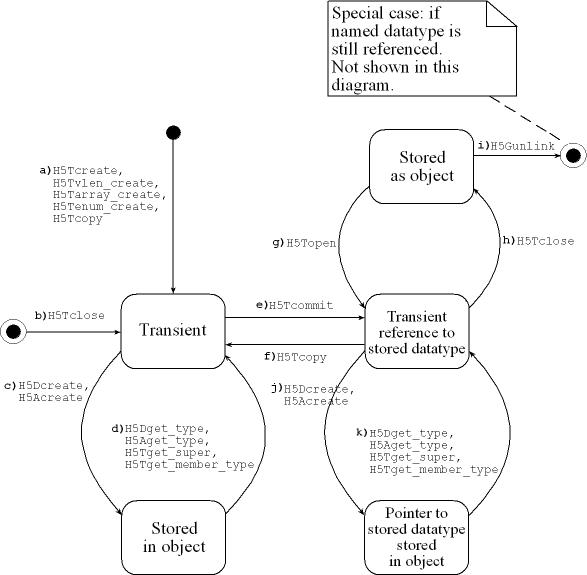
\includegraphics[scale=0.60]{images/datatype_life_cycle.png}
\caption{Datatype life cycle}
\label{fig:datatype-life-cycle}
\end{figure}

If a transient datatype is committed, the \texttt{vol\_obj} field of its shared information struct is populated with a copy of itself that is stored on disk, and the datatype's handle becomes a transient reference to the stored datatype. A transient reference to a stored datatype is also obtained when querying the datatype of an object with a committed datatype.

A committed datatype will be slated for removal from the file by \texttt{H5Ldelete} (or the deprecated \texttt{H5Gunlink}) if no other objects reference it. If it is unlinked and the objects that reference it are later deleted, the datatype's memory will be marked as free by the free space manager at that time. 

    \item Alignment

Different platforms may have different byte alignment restrictions when placing types within structures. The \texttt{HOFFSET} macro should be used when creating a compound type in order to align the inserted fields with any automatically added bytes of padding. 

Alignment of stored fields is not necessary when storing data structures on disk, and so the padding bytes can be removed to increase storage efficiency by `packing' the datatype. Compound types can be packed with \texttt{H5Tpack} to create storage-optimized unaligned versions. \texttt{H5Tpack} directly modifies the datatype it is given, so it should usually be preceded by \texttt{H5Tcopy}. Note that a packed datatype will usually be unable to describe in-memory data.

    \item Endianess
    
A platform that stores the most significant byte of a number at the smallest memory address is 'big-endian', and a platform that stores the least significant byte at the smallest memory address is 'little-endian.' The HDF5 library determines during its configuration which convention the current platform uses, and stores that as the 'native' convention, used by predefined types such as \texttt{H5T\_NATIVE\_INT}.
        
    \item Datatype hard and soft conversions

Each datatype conversion function has a 'hard' or 'soft' persistence. The persistence of a conversion function determines what source and destination datatypes it will be used for. A hard conversion function will only be used for the specific datatypes it is registered for, while a soft conversion function will be applied to any datatypes that match the classes of the source and destination types it is registered for.

A new hard conversion function will overwrite any previous conversion functions for the provided types, and a new soft conversion function will overwrite the conversion functions for any types to which it is applicable that do not already have a hard conversion function.
        
    \item Variable length datatypes

Because the total amount of storage space needed for objects with a variable length datatype cannot be known ahead of time and may change, data with a variable length type is stored in the file's global heap, rather than in the data object. The metadata describing the variable-length type itself is stored in a Datatype Message in an object's header, just as for non-variable-length datatypes. 

As a derived type, a variable-length datatype stores a pointer to its base datatype in the \texttt{parent} field of its shared type information structure. 

    \item Reference datatypes

Reference types are internally handled slightly differently than other 'complex' datatypes (e.g. compound, array, variable length types). Rather than having a unique structure which is a possible value of the union \texttt{u} in the shared type information structure, reference datatype objects are considered 'atomic', and are represented by a \texttt{H5T\_atomic\_t} instance. Reference-specific information is then stored under the \texttt{r} field of the atomic datatype structure's own union \texttt{u}.

    \item Datatype serialization

Datatype serialization to and from datatype messages is performed by the encode/decode callbacks on the datatype message class, \texttt{H5O\_\_dtype\_(encode/decode)}. It is also exposed as part of the API through \texttt{H5Tencode/H5Tdecode}. For atomic datatypes, encoding and decoding are accomplished non-recursively. For compound
types, a separate recursive call encodes each member field of the overall datatype. For arrays, variable-length types and enums a single recursive call is used to encode the base type.

    \item Addition of new native types
    
While the library allows applications to create their own custom datatypes, there are some reasons why a native datatype may be desired. For example, two applications may make different choices for how to implement complex numbers as a compound datatype, decreasing the portability of the data. For those interested in the process of introducing new native datatypes to the library, RFC THG 2015-04-29 ~\cite{rfc20150429}, specifically section 3.1, details which parts of the library and tools must be changed for compatibility with a new native datatype.

\end{itemize}

\subsection{Data Filters (\texttt{H5Z})}

%|  Name  | TODO | ONGOING | DONE |
%|--------|------|---------|------|
%| Dana   | x    |         |      |
%| Gerd   | x    |         |      |
%| Glenn  | x    |         |      |
%| Jordan | x    |         |      |
%| Luke   | x    |         |      |
%| Matt   |      |         |  x   |
%| Neil   | x    |         |      |
%| Scot   | x    |         |      |

\todo[inline]{Owner: Glenn -- Priority: Medium -- Effort: M -- Completion: 80\%}

\begin{itemize}
    \item Data filter pipeline

Data filters are used to manipulate data. The HDF5 library provides several built-in filters to allow for compression ({\footnotesize\texttt{H5Z\_FILTER\_DEFLATE}, \texttt{H5Z\_FILTER\_SZIP}, \texttt{H5Z\_FILTER\_NBIT}, \texttt{H5Z\_FILTER\_SCALEOFFSET}}), shuffling ({\footnotesize\texttt{H5Z\_FILTER\_SHUFFLE}}), and error checking ({\footnotesize\texttt{H5Z\_FILTER\_FLETCHER32}}). While filters can be used individually, they can also be stacked into a filter pipeline. Filters for contiguous datasets are not currently supported because implementing random access for partial I/O is difficult, and compact datasets are also not supported because the potential gains from filters are negligible on such small datasets. Theoretically, the maximum number of filter applications should be unlimited, but because each filter uses a bit in a 32-bit field, the actual maximum number of filter applications is 32. 

Users can also define their own filters to customize data processing further, which provides a high degree of flexibility for tailoring the pipeline to specific needs. As long as the filter is associated with a dataset upon the creation of that dataset, can be used with chunked data (\texttt{H5D\_CHUNKED}), and is applied to each individual chunk in a \texttt{H5D\_CHUNKED} dataset, then the custom filter may be registered and used. This is done through a two-step process. First, three callback functions must be written. The first is \texttt{H5Z\_can\_apply\_func\_t}, which checks against the dataset's dataset creation property list, datatype, and dataspace. The next is \texttt{H5Z\_set\_local\_func\_t}, which sets local flags and fields using the aforementioned three parameters. The last is \texttt{H5Z\_func\_t}, which takes in a bit vector of flags, the number of elements in the array of auxiliary data for the filter, the array of auxiliary data itself, the number of bytes in the filter buffer, the size of the filter buffer, and the filter buffer itself, and uses the fields set by the previous method to return the altered buffer back to the user along with its size. 

Once the above callbacks have been defined, the filter must be registered using \texttt{H5Zregister()}. \texttt{H5Zregister()} takes a pointer to a buffer for the class data structure and returns a \texttt{H5Z\_class\_t} (a two-byte identification number), which can be either \texttt{H5Z\_class1\_t} or \texttt{H5Z\_class2\_t}. 

\texttt{H5Z\_class\_t} is a macro that maps to either of the above two versions depending on the needs of the application. \texttt{H5Z\_class\_t}s start from 0-255, and these values are reserved for official HDF5 filters such as the ones listed above. 256-511 include the numbers that may be used for temporary testing. Lastly, 512-65535 is reserved for future assignments. If the filter is set as optional, then the library will skip the filter while proceeding through the filter pipeline.

At the center of the data filter pipeline is \texttt{H5Z\_pipeline()}, which is what carries out the pipeline. This method processes filters in definition order, or reverse order if the \texttt{H5Z\_FLAG\_REVERSE} flag is set. It takes in a \texttt{H5O\_pline\_t}, an unsigned int for flags, an array of unsigned ints for a filter mask, a \texttt{H5Z\_EDC\_t}, an \texttt{H5Z\_cb\_t} instance, a \texttt{size\_t} nbytes, which holds the number of bytes to filter, a \texttt{size\_t} buf\_size, which holds the total allocated size of the buffer, and buf, which is the buffer itself. This method will first check if the filter is registered, and if it is not already registered, it will try to load it dynamically and then register it. Once this is done, it will go through the list of filters in definition order and attempt to apply each filter to the data.

It is important to note that functions that allocate and free memory must be treated with care, since if there is a mismatch between the memory allocators used in the library and any memory that might be moved around by a filter, there may be problems. This issue can be resolved via the \texttt{H5allocate\_memory} and \texttt{H5free\_memory} functions, but if these methods are used, then the filter would have to be linked to a specific library version, which may be problematic. 

    \item Data transforms

Data transforms are also included in \texttt{H5Z}, and can be accessed via methods like \texttt{H5Z\_xform\_eval} on trivial transformations or \texttt{H5Z\_\_xform\_eval\_full} on complex transformations. This is done through the use of \texttt{H5Z\_node} to hold the parse tree and \texttt{H5Z\_token} to hold the original expression, current token values, and previous token values. Each \texttt{H5Z\_node} contains a left child, right child, \texttt{H5Z\_token\_type} to hold the type, and a \texttt{H5Z\_num\_val} to hold the value. Additionally, it includes macros for several different operations such as \texttt{H5Z\_XFORM\_DO\_OP1}, each of which is used in \texttt{H5Z\_\_xform\_reduce\_tree} to simplify parse trees, which is used when evaluating transformations.

\end{itemize}

\subsection{Dataspaces (\texttt{H5S})}

%|  Name  | TODO | ONGOING | DONE |
%|--------|------|---------|------|
%| Dana   | x    |         |      |
%| Gerd   | x    |         |      |
%| Glenn  | x    |         |      |
%| Jordan | x    |         |      |
%| Luke   | x    |         |      |
%| Matt   |      |         |  x   |
%| Neil   | x    |         |      |
%| Scot   | x    |         |      |

%\todo[inline]{Owner: Neil -- Priority: High -- Effort: L  -- Completion: 100\%}

A dataspace in HDF5 consists of two parts: an extent and a selection within that extent. They are mostly handled separately in the HDF5 library and only tied together at the top level of the structure. Extents are fairly trivial, consisting of a rank (number of dimensions) and size in each of these dimensions.

Selections are handled inside the \texttt{H5S} (dataspace) package with a flexible, class-like interface consisting of a \texttt{struct} of function pointers which must be implemented by each selection type. Currently, four selection types are implemented in HDF5: none, all, hyperslab, and point. `None' refers to a selection with no elements selected, while `all' refers to a selection of every element in the extent. Hyperslab selections are created using combinations of (\texttt{N}-dimensional) rectangular blocks, and a point selection is a list of individual elements. Point selection is the only selection type where the elements may be selected out of order, that is, the order of elements within the selection might not match the order of those elements within the serialized extent. Hyperslab blocks may be added in any order, but after combination, the order of the elements within the selection matches the order within the extent, as shown in Figure~\ref{fig:serial-offsets}. The order of elements within the extent is the same as the ordering of memory elements in a multi-dimensional array for the programming language used. Examples in this section use row-major ordering, as used by C.

\begin{figure}[h]
\centering
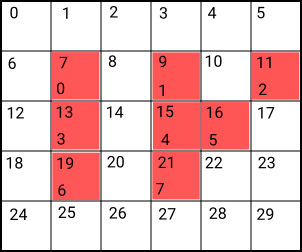
\includegraphics[scale=0.8]{images/Dataspace_serial_offsets.png}
\caption{A dataspace extent and selection (red) within the extent. The serialized offset within the extent is in the upper left of each element and the serialized offset within the selection is in the lower left.}
\label{fig:serial-offsets}
\end{figure}

\begin{itemize}
    \item Dataspace in-memory objects

The dataspace object in HDF5 is represented with the struct \texttt{H5S\_t} containing two fields, \texttt{extent} and \texttt{selection}, exactly mirroring the conceptual model above.

The extent field contains the dataspace extent (number of dimensions and number of elements in each dimension), as well as the type of extent, number of elements (for convenience), and information needed to encode the extent to an object header message.

The selection field contains the selection class (type) struct, which consists of a list of function pointers that the selection class uses to implement the necessary selection callbacks. The selection field also contains information on the selection offset, number of elements selected (again for convenience), and the information describing the actual shape of the selection, which depends on the selection class.

    \item Dataspace extents

Dataspace extents can be one of three types: scalar (\texttt{H5S\_SCALAR}), simple (\texttt{H5S\_SIMPLE}), and null (\texttt{H5S\_NULL}). A scalar dataspace extent represents a single element, a simple dataspace extent represents an N-dimensional array of elements, where N is between 1 and 32, and a null dataspace represents no elements. Simple dataspaces have an array size in each dimension, and also a maximum array size in each dimension (or \texttt{H5S\_UNLIMITED} to represent no maximum size). The size of each dimension can be changed with a call to \texttt{H5Sset\_extent()}, though each dimension size cannot be set to larger than the corresponding maximum dimension size. The maximum dimension sizes and the rank (number of dimensions) cannot be changed.

    \item Dataspace selections

Dataspace selections are used to select a subset of elements within the dataspace extent. They can be used to perform an operation on these elements, or simply to describe the subset (such as with a region reference). There are multiple types of selections, each of which must be defined by implementing the selection class, consisting of a series of callback functions that must be implemented. In addition, there are other functions that deal with individual selection types directly (such as \texttt{H5Sselect\_hyperslab()}) or that deal with multiple selection types (such as \texttt{H5Sselect\_project\_intersection()}).

    \item Hyperslab selections

Hyperslab selections represent an N-dimensional hyperrectangle of elements within the extent (where N is equal to the rank of the extent), a regular pattern of these hyperrectangles, or a combination of multiple hyperrectangles and/or patterns.

Hyperslabs are primarily constructed through the API using \texttt{H5Select\_hyperslab()}, which takes, as parameters, \texttt{start}, \texttt{stride}, \texttt{count}, and \texttt{block}, all of which are arrays of length matching the rank of the dataspace extent. \texttt{start} indicates the element at which the hyperslab begins (i.e. the element closest to position 0 in each dimension). \texttt{stride} indicates the spacing between the starting position of regularly spaced blocks in each dimension. \texttt{count} indicates the number of regularly spaced blocks in each dimension. \texttt{block} indicates the size of each regularly spaced block. In addition, hyperslabs can be combined in different ways using the \texttt{op} parameter, potentially yielding hyperslabs that cannot be represented using a single set of \texttt{start}, \texttt{stride}, \texttt{count}, and \texttt{block} arrays.

Internally, hyperslabs are represented in one of two ways. Hyperslabs that can be represented using a single set of \texttt{start}, \texttt{stride}, \texttt{count}, and \texttt{block} arrays are called \textit{regular} hyperslabs and are represented using these arrays. Other, irregular, hyperslabs are represented using a data structure called a \textit{span tree}.

A span tree is a multidimensional linked-list representing spans of selected elements. It is implemented using the \texttt{H5S\_hyper\_span\_info\_t} and \texttt{H5S\_hyper\_span\_t} structs. The entry point for a span tree is a \texttt{H5S\_hyper\_span\_info\_t} which is the head of the linked list of spans (each represented by a \texttt{H5S\_hyper\_span\_t}) in the slowest changing dimension of the dataspace. Each span contains a \texttt{down} pointer to a \texttt{H5S\_hyper\_span\_info\_t} in the next fastest changing dimension.

To more easily understand span trees, it is useful to start at the fastest changing dimension. In this dimension, there are no \texttt{down} pointers, and each span consists only of a low and high bound (coordinates in the fastest changing dimension of the dataspace), and a pointer to the next span. This forms a one-dimensional pattern of "dashes". In the next dimension up, this process is repeated, except instead of each span selecting a list of elements, it selects a list of these dashed patterns. An example of a span tree representation of a selection in a 2-D dataset can be found in Figure~\ref{fig:span-trees}.

\begin{figure}[h]
\centering
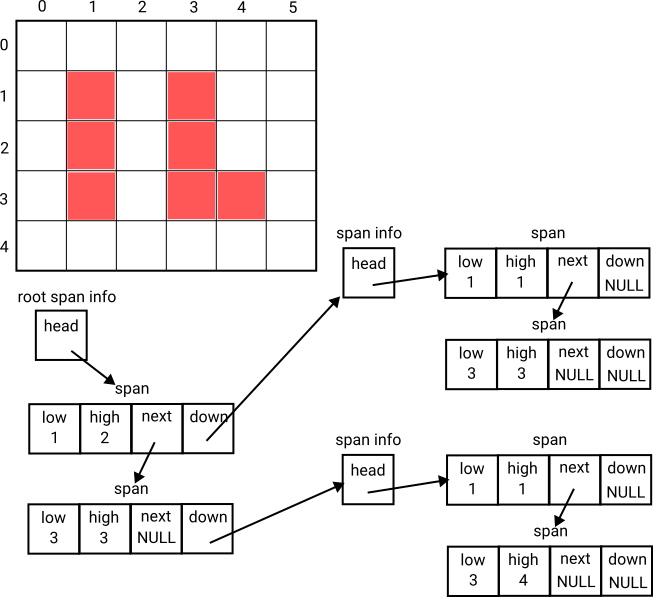
\includegraphics[scale=0.8]{images/Span_trees.png}
\caption{An illustration of span trees for a 2-D selection.}
\label{fig:span-trees}
\end{figure}

Hyperslabs can have either a regular description (start, stride, count, and block), a span tree description, or both.  Operations that are performed on hyperslabs need to be able to handle all of these cases. Some operations will construct a span tree for a regular on entry in order to simplify implementation (so it only needs to be implemented for span trees), though if an operation can be performed on a regular hyperslab directly that is generally more efficient. If a span tree is changed for a regular hyperslab it must be assumed it is no longer regular so the start, stride, block, and count are marked invalid. Also, after operations that can change a hyperslab, they will generally check if the hyperslab is regular and compute valid start, stride, block, and count values if so.

    \item Point selections

Point selections are a simple linear list of individual elements that are selected within the dataspace extent. They are implemented using a simple linked list of N-dimensional coordinates of each point. While conceptually simple, the fact that the points can be selected out of order with respect to the ordering of elements within the extent causes complications. The parallel code needs to take special care to reorder point selections as needed to obey MPI semantics, and virtual datasets do not support point selections at all. It is worth noting that it would not take much more work to implement point selection support for virtual datasets.

    \item Selection iterators and iteration operations

A selection iterator is a structure used to perform operations that iterate over a dataspace, such as generating offset/length pairs of selected elements (\texttt{H5S\_get\_seq\_list()}) or making a callback for each element selected (\texttt{H5S\_select\_iterate()}. The selection iterator includes another generic interface, \texttt{H5S\_sel\_iter\_class\_t}, that contains callback functions that must be implemented by each selection type. In addition, hyperslab and point selections store their own data in the selection iterator struct. These callbacks are used by the higher level code in \texttt{H5Sselect.c} to implement these operations. The iterator operations can also be called directly by external packages.

    \item Projections and the "shapesame" case

When performing I/O with selections, the library is given an extent and selection for the memory buffer, and a selection for the file (the extent for the file is implied by the dataset size). For contiguous datasets, the generic case here can be easily handled using selection iteration. The elements selected in the memory can be matched up 1-to-1 with elements selected in the file by the order within the selection, so the Nth element selected in memory is written to/read from the Nth element selected in the file. For chunked datasets, however, this becomes more complicated. The dataset in the file is broken up into chunks that may not be contiguous within the serialized (flattened) extent of the dataset, but the memory buffer is not broken up in the same way (indeed, the memory buffer need not have the same extent or even rank as the dataset). We therefore need to break the file selection up into a series of selections, one for each chunk. It is easy to do this using selection interfaces that compute the intersection of two selections. However, we also need to compute the selection in memory that corresponds to the selection within each chunk. Since the chunks may not be contiguous in the serialized extent, we can no longer rely on the 1-to-1 mapping used for contiguous datasets.

However, there is a shortcut we can take when a certain common condition is fulfilled. Often, the selections in the memory and file have the same shape, possibly with some offset between the two. If this is the case, we can simply, for each chunk, compute the intersection ("and") of that chunk with the file selection, then copy that intersection to the memory space, and apply any offset computed from comparing the overall file and memory selections. This copied intersection, called a projection, is now a selection containing the memory elements that match, in the correct order, the file elements selected that are in the current chunk. The dataset code then uses these file and memory chunk selection pairs to construct the I/O operation. The function used to check if two selections have the same shape is \texttt{H5S\_select\_shape\_same()} (wrapped by the macro \texttt{H5S\_SELECT\_SHAPE\_SAME()}), and the function used to construct the projected dataspace is \texttt{H5S\_select\_construct\_projection()}.

While the selections must have the same shape for this case to work, it is actually possible for the extents to be different ranks. If we have selections \(A\) and \(B\), with extents of rank \(M\) and \(N\), respectively, where \(M>N\), then \(A\) and \(B\) have the same rank if and only if selection \(A\) spans only a single element in the slowest changing \(M-N\) dimensions, and if \(A\) and \(B\) are identical in the fastest changing \(N\) dimensions, possibly with a constant offset. The library does not currently try to identify cases where the selections could be topologically identical by unrolling one or more dimensions, as this would require a different algorithm to construct the projection. They must actually be the same in the shared dimensions.

    \item The project intersection operation

The operation \texttt{H5Sselect\_project\_intersection()} and its corresponding private interface, \texttt{H5S\_select\_project\_intersection()}, is robust but can be confusing due to its complexity. This function takes three dataspaces, each with a selection, and outputs a fourth. Internally, this function is currently only used to implement virtual datasets, but it is also used by some VOL connectors to implement generic I/O with selections on chunked datasets. It may be beneficial in the future to implement chunked I/O using this operation when the shapesame case does not apply.

%\todo[inline]{GH: I think we should make a distinction between `chunks', which is a storage concept, and their counterparts in the dataspace context. How about we call them `tiles'? A tile is the logical place of a chunk in a dataspace. We definitely need a figure to show people an example of how the generic case falls apart.} 

In the general case for chunked dataset I/O we cannot simply copy the intersection from file to memory as in the shapesame case. The projected chunk selection in memory can be of a totally different shape from the chunk selection in the file. Instead, we can, for each chunk, calculate the offsets of the selected elements in that chunk within the serialized file selection, then select the elements in the memory space with the matching offsets within the serialized memory selection. This resulting memory chunk selection, which is a subset of the overall memory selection, contains the elements selected in the chunk being processed. An example showing this process for a single chunk of a two-dimensional dataset is shown in Figure~\ref{fig:project-intersection-chunk}. This process is repeated for every chunk that contains any selected elements. 

\begin{figure}[h]
\centering
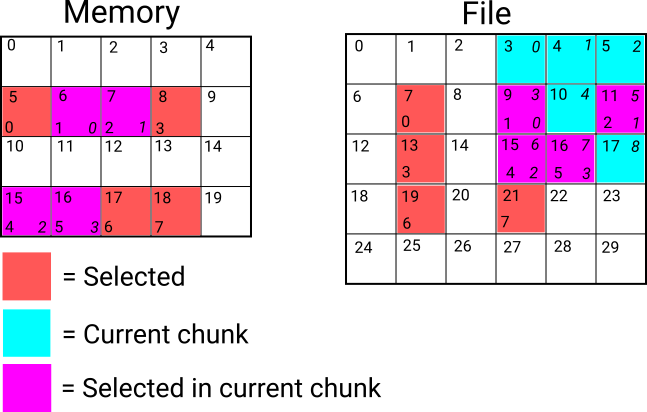
\includegraphics[scale=0.8]{images/Project_intersection_chunk.png}
\caption{A project intersection operation used for chunk I/O. The serialized offset within the extent is in the upper left of each element, the serialized offset within the selection is in the lower left, the serialized offset within the chunk is in the upper right, and the serialized offset within the intersected space is in the lower right. The result of the operation is the "selection in current chunk" (pink) in memory.}
\label{fig:project-intersection-chunk}
\end{figure}

The general chunked I/O case is supported by \texttt{H5S\_select\_project\_intersection()}, though that function also supports other use cases. \texttt{H5S\_select\_project\_intersection()} does not require that the selection representing the chunk in the above example be rectangular, it can be any selection that can be represented using the HDF5 API. In this function's terminology, the file selection (in the example) is referred to as the "source space", the memory selection is referred to as the "destination space", and the chunk selection is referred to as the "source intersect space". While the above description implies an element-by-element algorithm for calculating the source intersect space, in the case of hyperslabs (possibly combined with an all selection), the library uses span trees to be able to process the selection multiple elements at a time, which is generally much quicker. The project intersection operation can be thought of as projecting the intersection of the source space and the source intersect space onto the destination space, where there is a one-to-one mapping between the source space and the destination space (though they need not have the same shape).

This facility is not currently used by the native library to perform chunk I/O. If the shapesame case does not apply, the library iterates element by element over the selections in the dataset package. However, we would like to investigate using this function for the non-shapesame case in the native library, as we believe it may improve performance. The library currently uses this facility to implement virtual datasets, and some VOL connectors use it to implement chunked I/O. At some point in the future, we may wish to unify the shapesame projection and the project intersection operations.

    \item Parallel (MPI) operations

The dataspace code is also used to translate dataspace selections into MPI datatypes, which is central to the MPI I/O implementation. This functionality is present in \texttt{H5Smpio.c} and is called by functions in \texttt{H5Dmpio.c} as well as directly from the MPIO file driver in \texttt{H5FDmpio.c}. These functions are mostly straightforward, with different algorithms for point, regular hyperslab, and hyperslab span tree selections.

\end{itemize}

\subsubsection{Source files in the \texttt{H5S} package}

\begin{table}[!ht]
\begin{tabular}{||c|l||}
\hline
\textbf{Source File} & \textbf{Description} \\  [0.5ex] 
\hline\hline
\texttt{H5Spublic.h} & Public dataspace API \\
\texttt{H5Sprivate.h} & Private header (internal dataspace API) \\
\texttt{H5Spkg.h} & Package header (package private symbols) \\
\texttt{H5Smodule.h} & Package initialization boilerplate and User's Guide \\
\texttt{H5S.c} & Public API functions, package initialization, other core functions \\
\texttt{H5Sall.c} & `All' selection type \\
\texttt{H5Sdbg.c} & Debugging functions \\
\texttt{H5Sdeprec.c} & Deprecated functions \\
\texttt{H5Shyper.c} & `Hyperslab' selection type \\
\texttt{H5Smpio.c} & Parallel functionality for constructing MPI datatypes \\
\texttt{H5Sall.c} & `None' selection type \\
\texttt{H5Spoint.c} & `Point' selection type \\
\texttt{H5Sselect.c} & Operations on general hyperslab selections. Often just passes down to the specific selection type. \\  
\texttt{H5Stest.c} & Functions used only by the regression test suite \\
\hline
\end{tabular}
%\caption{}
\label{table:H5Scode}
\end{table}

%\subsubsection{Other source files referenced in this section}

%\begin{table}[h!]
%\begin{tabular}{||c|l||}
%\hline
%\textbf{Source File} & %\textbf{Description} \\  [0.5ex] 
%\hline\hline
%\texttt{H5Dmpio.c} & \ldots \\
%\texttt{H5FDmpio.c} & \ldots \\
%\hline
%\end{tabular}
%\caption{}
%\label{table:H5Smisc}
%\end{table}

% \subsection{References (\texttt{H5R})}
% \todo[inline]{Owner: ??? -- Priority: Low -- Effort: M}

\begin{comment}

\subsection{Property Lists (\texttt{H5P})}


%|  Name  | TODO | ONGOING | DONE |
%|--------|------|---------|------|
%| Dana   | x    |         |      |
%| Gerd   | x    |         |      |
%| Glenn  | x    |         |      |
%| Jordan | x    |         |      |
%| Luke   | x    |         |      |
%| Matt   | x    |         |      |
%| Neil   | x    |         |      |
%| Scot   | x    |         |      |

\todo[inline]{Owner: Dana -- Priority: Medium -- Effort: M -- Completion: 0\%}

\begin{itemize}
    \item Property list in-memory objects
    \item Property list classes and inheritance
    \item Property creation
    \item Setting and getting properties
    \item Property list serialization
\end{itemize}

% \subsection{Plugins (\texttt{H5PL})}
% \todo[inline]{Owner: Allen(?) -- Priority: Low -- Effort: S}

% There are three kinds of plugin in the library:

% \begin{itemize}
%     \item Filters
%     \item VOL connectors
%     \item VFD plugins
% \end{itemize}

% Each of these plugin categories is handled identically by the library, using a common plugin loading and caching harness.

% The plugin cache is so straightforward, it doesn't even warrant a drawing - it's just a simple collection of previously loaded plugin objects, each of which stores its category (e.g., filter), a unique key that can be used to identify the plugin (typically an integer ID, but might also be a name), and the plugin itself. When the library needs to search for a plugin, it simply checks the cache to see if the plugin has already been loaded, and, if not, tries to find and load the plugin via the plugin search path(s), storing it in the cache on success.

% The library also maintains a list of plugin paths. There is a platform-dependent default plugin path and API calls exist that allow users to manipulate the plugin path list. As with the plugin cache, the collection of plugin paths is common across all categories of plugins (though this may change in the future).

% Users can also set a plugin mask, which can be used to selectively disable plugin loads for each category of plugin. This mask is stored at the library level.

% The mechanism for creating an HDF5 library plugin is documented elsewhere. All plugins implement an interface (defined in H5PLextern.h) that allows the library to load and introspect plugins. Each category of plugins will additionally require the implementation of a number of callbacks.

% In the source code, plugins are handled via the H5PL package. Please see the package documentation in the repository for implementation details.
\end{comment}
\subsection{Virtual Object Layer (\texttt{H5VL})}\label{ref:vol}

%|  Name  | TODO | ONGOING | DONE |
%|--------|------|---------|------|
%| Dana   | x    |         |      |
%| Gerd   | x    |         |      |
%| Glenn  | x    |         |      |
%| Jordan | x    |         |      |
%| Luke   | x    |         |      |
%| Matt   | x    |         |      |
%| Neil   | x    |         |      |
%| Scot   | x    |         |      |

%\todo[inline]{Owner: Luke -- Priority: Medium -- Effort: L -- Completion: 100\%}

The virtual object layer (VOL) is an abstraction layer that intercepts all I/O-related calls in HDF5 and forwards them to custom callbacks. VOLs take as input high-level knowledge of the data format and data access characteristics, enabling the development of custom data operators, application-aware caching and logging, monitoring algorithms, specialized file formats, and integration with new storage technologies. Applications depending on HDF5 can leverage VOL plugins to meet their specific data requirements without code change through the use of environment variables and dynamic linking. This combination of extensibility and transparency positions HDF5 as an enduring data storage solution capable of adapting to a diversity of workloads and future innovations in storage technologies.

VOL connectors are highly flexible in the functionality they can encompass. Connectors can be applied in both serial and parallel HDF5, unlike VFDs. There are two general categories of VOL connector.
\begin{enumerate}
    \item \textbf{Pass-through VOL Connectors}: Forward data to a future VOL connector. An example is context-aware data caching which can intelligently place or prefetch data without change in the overall file format. Alternatively, an adaptive compression makes use of the data format to intelligently select a compression library. Note that HDF5 Filters have some similarities to pass-through connectors, but filters are limited to the native VOL. It is non-trivial to reuse filters in custom connectors. Other examples include the async and external VOLs in HDF5.
    \item \textbf{Terminal VOL Connectors}: The final VOL connector in a list of VOL connectors. Intended to be used for low-level data storage. An example is the HDF5 native VOL, which constructs the well-known HDF5 (*.hdf5) file format in storage. Other examples include the DAOS and S3 VOLs. Both DAOS and S3 are object stores, differing from traditional POSIX-compliant filesystems. HDF5 can now reliably store and retrieve data in these systems.
\end{enumerate}

VOL connector authors should be aware of the concurrency model of HDF5 when developing their VOLs:
\begin{enumerate}
    \item \textbf{Multi-Process Concurrency}: In parallel HDF5, Not all VOL functions are compatible with MPI\_Barrier. This is because not all I/O performed in HDF5 is collective. I/O is collective only when the application specifically passes H5FD\_MPIO\_COLLECTIVE flag or when the VOL function is related to internal HDF5 metadata updates.
    \item \textbf{Multi-Thread Concurrency}: VOL connectors will never be called from multiple threads at the same time in HDF5. This is because HDF5 uses a global lock when performing I/O. All VOLs in the list of VOLs will be executed in sequence before the lock is released. To improve concurrency, a VOL connector can leverage asynchronicity and internally spawn and manage its own worker threads for background tasks.
\end{enumerate}

\subsubsection{The VOL Class Structure}

VOL connectors are defined using the VOL class struct (\texttt{H5VL\_class\_t}), which contains function pointers to various HDF5 operation overrides and identifying information. VOLs are intended to follow the singleton design pattern. Typically the VOL class is declared as a static global variable in the VOL source file so that VOL functions can access the variable easily without explicitly passing it in. VOLs can choose to leave most functions unimplemented by setting them to NULL.

The VOL class has a few parameters regarding the identification and versioning of the VOL.
\begin{enumerate}
    \item \textbf{VOL connector ID}: A globally unique integer constant of type \texttt{H5VL\_class\_value\_t} that can be used to locate the VOL.
    \item \textbf{VOL name}: A globally unique semantic string that can be used to locate the VOL. While not technically erronous, spaces in the VOL name should be avoided since it increases the complexity of VOL initialization through environment variables.
    \item \textbf{VOL connector version}: An integer indicating the version of this VOL. This is mainly intended to help users ensure they are linking against the correct version of the VOL code.
    \item \textbf{VOL class struct version}: The version of the class struct being implemented. Different HDF5 versions have different class struct definitions. This allows HDF5 to determine whether the VOL was designed for the particular HDF5 version a user application is compiled against.
    \item \textbf{VOL capability flags}: Various flags indicating the supported functionality of the VOL. This can include information such as support for provenance, hard links and soft links, and attribute references.
\end{enumerate}

VOLs provide two functions for initializing and finalizing VOL classes.
\begin{enumerate}
    \item \textbf{initialize}: a method called to initialize the VOL connector
    \item \textbf{terminate}: a method called to free data allocated by VOL connector
\end{enumerate}

There are 9 general classes of functions that can be overridden for the HDF5 data model:
\begin{enumerate}
    \item \texttt{H5VL\_info\_class\_t}: Query the VOL connector's custom information. This can include methods for comparing two VOL connectors and allocating/freeing any custom state held by the VOL connector.
    \item \texttt{H5VL\_wrap\_class\_t}: Only for pass-through connectors. Used to manage the translation between the HDF5 library's internal representation of objects and the user's representation.
    \item \texttt{H5VL\_attr\_class\_t}: Override the HDF5 attribute APIs (H5A*), such as \texttt{H5Acreate}.
    \item \texttt{H5VL\_dataset\_class\_t}: Override the HDF5 dataset APIs (H5D*), such as \texttt{H5Dread}.
    \item \texttt{H5VL\_datatype\_class\_t}: Override the HDF5 datatype APIs (H5T*), such as \texttt{H5Tcreate}.
    \item \texttt{H5VL\_file\_class\_t}: Override the HDF5 file APIs (H5F*), such \texttt{H5Fcreate}.
    \item \texttt{H5VL\_group\_class\_t}: Override the HDF5 group APIs (H5G*), such as \texttt{H5Gcreate}.
    \item \texttt{H5VL\_link\_class\_t}: Override the HDF5 link APIs (H5L*), such as \texttt{H5Lexists}.
    \item \texttt{H5VL\_object\_class\_t}: Override the HDF5 object APIs (H5O*), such as \texttt{H5Ocopy}.
\end{enumerate}

There are 4 general classes of function that can be overridden relating to infrastructure/services:
\begin{enumerate}
    \item \texttt{H5VL\_introspect\_class\_t}: Container/connector introspection class callbacks.
    \item \texttt{H5VL\_request\_class\_t}: Asynchronous request class callbacks.
    \item \texttt{H5VL\_blob\_class\_t}: Blob class callbacks.
    \item \texttt{H5VL\_token\_class\_t}: VOL connector object token class callbacks.
\end{enumerate}

\subsubsection{VOL Registration}

It is mandatory for every VOL to implement and register the \texttt{H5VL\_class\_t} struct. This struct outlines the set of methods the VOL overrides. There are various ways to register the \texttt{H5VL\_class\_t} struct. In the library, there are three API routines for VOL registration:
\begin{enumerate}
    \item \texttt{H5VLregister\_connector}: takes as input the class struct pointer directly and registers it with HDF5
    \item \texttt{H5VLregister\_connector\_by\_name}: use the plugins interface (H5PL) to locate the VOL by the VOL name
    \item \texttt{H5VLregister\_connector\_by\_value}: use the plugins interface (H5PL) to locate the VOL by the connector ID
\end{enumerate}
During registration, the \texttt{initialize} function defined in the VOL class struct will be called if it is non-NULL. This function does not take any parameters -- except an empty property list. It is also only called once throughout the entire lifetime of the VOL and should be used to initialize any library or service required to be initialized exactly once. To pass variables to \texttt{initialize}, VOL authors should define custom environment variables and document them.

In addition, parameters can be passed to the VOL after registration using \texttt{H5VLconnector\_str\_to\_info}, which takes as input a string that is internally parsed by the VOL's custom \texttt{from\_str} function (defined in \texttt{H5VL\_info\_class\_t}). There is no required structure to this string, although it is best practice to avoid spaces and use `:'or `;' as separators for tokens. More complex parameters should be placed in custom environment variables instead. In \texttt{from\_str}, the parameter string will be parsed into a VOL-specific info struct, which can be accessed, copied, and queried using methods in \texttt{H5VL\_info\_class\_t}. An example of a parameter string to initialize a theoretical VOL named PFS that stores HDF5 data in a file on a PFS could be `username:/path/to/ssh/key:/path/to/file.txt'.

HDF5 can also transparently locate and register a VOL through the \texttt{HDF5\_PLUGIN\_PATH} and \\ \texttt{HDF5\_VOL\_CONNECTOR} environment variables. \texttt{HDF5\_PLUGIN\_PATH} tells HDF5 the directories to search for VOL libraries and \texttt{HDF5\_VOL\_CONNECTOR} holds a string containing the name and parameterization of a particular VOL to load. H5PL will split this string by spaces to determine the (VOL name, parameter) pair. Only a single VOL and its parameters can be specified using the environment variable. If the parameter string contains spaces, anything after the second space will be deleted. An example of \texttt{HDF5\_VOL\_CONNECTOR} for initializing the example PFS VOL could be `PFS username:/path/to/ssh/key:/path/to/file.txt', where PFS is the VOL name defined in the class struct. H5PL then automatically loads and registers the VOL, implicitly calling \texttt{H5VLregister\_connector\_by\_name} with the VOL name as input and \\ \texttt{H5VLconnector\_str\_to\_info} with the parameter string as input if it is not empty. \texttt{H5Pset\_vol} will then also be called to duplicate the info struct using the \texttt{copy} method defined in \texttt{H5VL\_info\_class\_t} and store in a property list tracked internally by HDF5. Generally, the info struct will be either passed directly to most VOL functions or queried from a property list.

To be compatible with H5PL, VOLs must implement the \texttt{H5PLget\_plugin\_type} and \\ \texttt{H5PLget\_plugin\_info} methods. HDF5 automatically searches for these methods and requires their signatures to be exactly correct. An example code is shown in Listing~\ref{lst:vol-init}.

\begin{listing}[!ht]
\centering
\caption{VOL plugin discovery code.}
\label{lst:vol-init}
\begin{minted}[linenos]{C}
static const H5VL_class_t H5VL_custom_vol_g = { /** method overrides */ }
H5PL_type_t H5PLget_plugin_type(void) {
  return H5PL_TYPE_VOL;
}
const void* H5PLget_plugin_info(void) {
  return &H5VL_custom_vol_g;
}
\end{minted}
\end{listing}

\subsubsection{VOL Organization}

\begin{figure}[!ht]
  \centering
  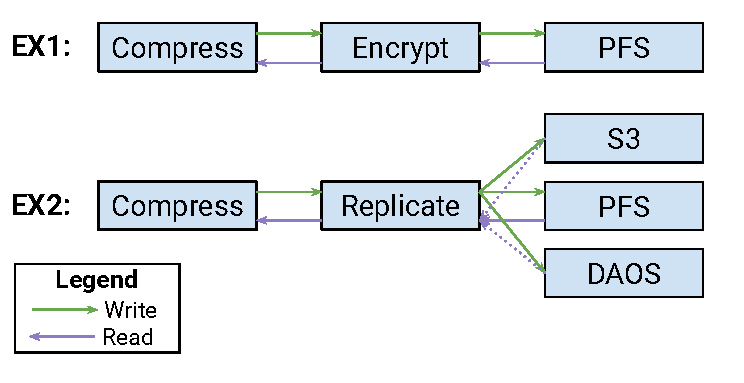
\includegraphics{images/tour_4_vol_dags.pdf}
  \caption{Depiction of data flow in VOL DAGs}
  \label{fig:vol-dag}
\end{figure}

VOLs can be conceptually organized as directed acyclic graphs (DAGs), although there is no specific DAG data structure in HDF5. Two examples of VOL DAGs and how data flows through them are shown in Figure~\ref{fig:vol-dag}. EX1 is a list of VOLs that compress, encrypt, and store the transformed data using a terminal PFS VOL. EX2 is a DAG of VOLs that compresses data and replicates the compressed data to numerous data repositories using terminal VOLs for S3, DAOS, and PFS. To create EX1, the parameter string would have to contain the information needed to register and initialize the compress, encrypt, and PFS VOLs. For example, \texttt{HDF5\_VOL\_CONNECTOR}=`compress zlib;encrypt:aes:/home/user/key.aes;PFS:/home/user/ex1.h5'. This string would be first passed to compress, where the relevant information needed to initialize the compress module will be parsed (zlib). Within the compress VOL, the name of the next VOL to create will be extracted (encrypt) and \texttt{H5VLregister\_connector\_by\_name} will be called using the remaining parameter string (aes:/home/user/key.aes;PFS:/home/user/ex1.h5). This will repeat recursively until each VOL is registered and defined. There is no specific functionality in HDF5 to initialize multiple VOLs at the same time -- it is the responsibility of a pass-through VOL developer to initialize any future VOLs it may depend on.

After initialization, I/O operations (e.g., dataset reads and writes) can be performed. Write operations are typically executed using preorder traversal (left-to-right for lists). For EX1, compression is first applied to the data, then encryption, and then persistent storage. EX2 is similar. Reads are typically executed using postorder traversal (right-to-left for lists). For EX1, data is first read from the PFS, decrypted, and then decompressed. In EX2, the replication VOL decides one of the three destinations (PFS, S3, or DAOS) to read data from, reads the data from that destination and then goes for decompression. In practice, these traversals are executed using recursion, where the first VOL registered is the root of the recursion. In EX1 and EX2, the root is the compress VOL. Pseudocode for the write and read operations for the compress VOL are depicted below in Listing~\ref{lst:compress-vol}. For writes, the input buffers stored in \texttt{buf} will be compressed into a new set of buffers \texttt{compressed}. The maximum size a compressed buffer can be is assumed to be the size of the original data, which is calculated using a custom \texttt{get\_data\_size} function. The compressed data is then forwarded to the next VOL using \texttt{H5VLdataset\_write}. Reads are similar, except the compressed data is first read using the next vol with \texttt{H5VLdataset\_read} and then decompressed into \texttt{buf}.

\begin{listing}[!ht]
\centering
\caption{Compression pass-through VOL code example.}
\label{lst:compress-vol}
\begin{minted}[linenos]{C}
typedef struct H5VL_compress_vol_info_t {
  int compress_method_;
  hid_t next_vol_id_;
  void *next_vol_info_;
} H5VL_compress_vol_info_t;
#define MAKE_TEMP_BUFFER \
  for (size_t i = 0; i < count; i++) { \
    next_objs[i] = objs[i]->next_vol_info_; \
    max_size[i] = get_data_size(mem_type_id[i], mem_space_id[i]); \
    compressed[i] = malloc(max_size[i]); \
  }
static herr_t H5VL_compress_vol_dataset_write(
    size_t count, void *dset[], hid_t mem_type_id[], hid_t mem_space_id[],
    hid_t file_space_id[], hid_t plist_id, const void *buf[], void **req) {
  H5VL_compress_vol_info_t **objs = (H5VL_compress_vol_info_t**)dset;
  void* next_objs[count]; void *compressed[count]; size_t max_size[count];
  MAKE_TEMP_BUFFER
  for (size_t i = 0; i < count; i++)
    compress(objs[i]->compress_method_, buf[i], max_size[i], compressed[i]);
  hid_t ret_value = H5VLdataset_write(
    count, (void**)next_objs, objs[0]->next_vol_id_, mem_type_id, 
    mem_space_id, file_space_id, plist_id, compressed, req);
  // Free compressed & return
}
static herr_t H5VL_compress_vol_dataset_read(/** Similar to write */) {
  H5VL_compress_vol_info_t **objs = (H5VL_compress_vol_info_t**)dset;
  void* next_objs[count]; void *compressed[count]; size_t max_size[count];
  MAKE_TEMP_BUFFER
  hid_t ret_value = H5VLdataset_read(/** Same as write */);
  for (size_t i = 0; i < count; ++i)
    decompress(objs[i]->compress_method_, compressed[i], max_size[i], buf[i]);
  // Free compressed & return
}
\end{minted}
\end{listing}


\subsubsection{Async VOLs}

VOLs can internally spawn thread pools to perform asynchronous operations and remove overhead such as locking and I/O stalls from the critical path. HDF5 does not provide a thread pool API and expects users will use an external threading library, such as pthreads or Argobots. Many VOL functions such as \texttt{H5VLdataset\_write} are either synchronous or asynchronous depending on if an HDF5 request struct is passed to it. \texttt{H5VL\_request\_class\_t} contains methods for waiting, canceling, completing, and freeing async requests. The VOL can define a custom request struct, taking as input the HDF request struct, and return it from VOL functions that behave asynchronously.

\subsubsection{Introspecting VOLs}

The introspection API provided by VOLs (\texttt{H5VL\_introspect\_class\_t}) provides several abilities to query properties of the VOL. \texttt{get\_conn\_cls} provides the ability to locate the class struct pointer for a VOL. The capability flags can be queried with \texttt{get\_cap\_flags}. Lastly, the \texttt{opt\_query} function allows for determining whether or not optional operations are supported by this VOL connector, such as a particular method in the \texttt{H5VL\_attr\_class\_t} struct. This is typically more fine-grained than the capability flag query. In addition, the \texttt{H5VL\_info\_class\_t} provides the ability to query the VOL's specific info struct, if the VOL defines one. The function \texttt{from\_str} allows the info struct to be converted into a human-readable string.

\subsubsection{Source files for \texttt{H5VL} developers}

\begin{table}[!ht]
\begin{tabular}{||c|l||}
\hline
\textbf{Source File} & \textbf{Description} \\  [0.5ex] 
\hline\hline
\texttt{H5VLpublic.h} & Public APIs for VOL registration and introspection \\
\texttt{H5VLconnector.h} & Public structs and APIs for VOL developers \\
\texttt{H5VLconnector\_passthru.h} & Public APIs for pass-through VOL developers \\
\texttt{H5VLpkg.h} & Internal APIs for VOL registration \\
\texttt{H5VLprivate.h} & Internal APIs for VOL calls \\
\texttt{H5VLmodule.h} & Internal macros for VOLs and documentation \\
\texttt{H5VL.c} & Implementation of H5VLpublic.h \\
\texttt{H5VLcallback.c} & Implementation of H5VLconnector.h and H5VLconnector\_passthru.h \\
\texttt{H5VLint.c} & Implementation of initialization functions in H5VLpkg.h \\
\texttt{H5VLdyn\_ops.c} & Implementation of optional functions in H5VLpkg.h \\
\texttt{H5VLtest.c} & Internal helpers for environment variable checks \\
\hline
\end{tabular}
%\caption{}
\label{table:VOL_src_files}
\end{table}

% \subsection{Event Sets and Asynchronous I/O (\texttt{H5ES})}
% \todo[inline]{Owner: ??? -- Priority: Medium -- Effort: S -- Completion: 0\%}

% \subsection{Minor/Convenience Interfaces (\texttt{H5[CS,RS,SL,UC,VM,WB]})}
% \todo[inline]{Owner: ??? -- Priority: Low -- Effort: M}

% \begin{itemize}
%     \item Skip lists (\texttt{H5SL})
%     \item Reference counted objects (\texttt{H5UC})
%     \item Reference counted strings (\texttt{H5RS})
%     \item Wrapped buffers (\texttt{H5WB})
%     \item Vector math (\texttt{H5VM})
%     \item Code stack (\texttt{H5CS})
% \end{itemize}


\section{Performance considerations}

%|  Name  | TODO | ONGOING | DONE |
%|--------|------|---------|------|
%| Dana   | x    |         |      |
%| Gerd   | x    |         |      |
%| Glenn  |      |    x    |      |
%| Jordan | x    |         |      |
%| Luke   | x    |         |      |
%| Matt   | x    |         |      |
%| Neil   | x    |         |      |
%| Scot   | x    |         |      |


%\todo[inline]{Owner: Neil -- Priority: High -- Effort: M -- Completion: 100\%}

\paragraph{Scope.}

\begin{itemize}
%    \item Library dos and dont's
    \item Skip list \& hash table use

The skip list is a simple in-memory data structure that allows O(log N) key/value insertion, lookup, and removal. Skip lists are used widely in the library for many tasks, including property list operations and I/O chunk selection (among many others). While skip lists should theoretically be efficient for these use cases as long as N does not grow extremely large, profiling has found that skip list operations are a frequent cause of library underperformance, even though the N values (number of properties, number of IDs) are not extremely large. We currently suspect this underperformance is due to the shape of the skip list data structures causing frequent CPU cache misses. More investigation is needed, and it may be possible to improve skip list performance with additional work. It is now recommended to avoid using the skip list in performance-critical sections of the code wherever possible. The primary motivation behind the context package (\texttt{H5CX}) is to avoid invoking skip list operations when handling property lists whenever possible. Unlike a classic skip list, HDF5's skip list is deterministic and does not use the random number generator and, therefore, will not interfere with the application's random numbers.

In order to improve performance, we have more recently incorporated the open-source uthash \cite{uthash} hash table into HDF5 and begun using it in places that previously would have used the skip list. A hash table offers, in general, O(1) insertion, lookup, and removal at the cost of higher memory usage. Therefore, a hash table can be expected to scale better than a skip list when handling large numbers of objects (again, at the cost of high memory usage). In practice, we have also found uthash to be more performant even with smaller numbers of objects. We recommend that developers use uthash instead of skip lists whenever possible and whenever memory usage is not critical.

When objects inserted into these structures need to be iterated over in key order, the advantage of uthash is less apparent. In this case, items in the skip list are already in the correct order, but the uthash hash table must be sorted with \texttt{HASH\_SORT}, which is an O(log N) operation. Likely, uthash is still faster in this case but needs more investigation.

    \item Allocations and deallocations

In order to minimize the number of calls to system memory management functions, the HDF5 library has implemented the free list (\texttt{H5FL}) package. This package serves as a cache of allocated memory blocks and is effectively an intermediate memory manager between the library and the operating system. Regular free lists are the most commonly used type of free list and serve as a cache of allocations of a single structure type. Other free list types are sequence, array, and factory free lists that are used for variable-sized allocations and are less frequently used, and may not be as efficient as simply using the system memory manager. More investigation is needed.

We have found mixed results when evaluating the performance of the free lists in HDF5. There is a configure option to disable free lists, sometimes leading to a greater performance with free lists disabled. It is likely that, when performing \texttt{calloc} operations, free lists are less efficient than simply using the system \texttt{calloc()} since the free list must \texttt{memset} the buffer, while the system can return a block from a page it knows has already been set to zero. For this reason, we recommend avoiding the use of \texttt{H5FK\_CALLOC()} whenever possible, and when that is not possible, consider using the system \texttt{calloc()} instead, unless there is reason to believe the free list will be faster. Note that, since you cannot mix free list and system memory management calls on the same memory block, if \texttt{calloc} is only needed some of the time, it might require profiling to determine which method is best.

    \item Parallel performance considerations

Parallel access can significantly improve raw data performance when HDF5 is used on a parallel file system. However, there are additional things to keep in mind to maximize performance and avoid falling into traps. For raw data, the most important decision to make is collective vs. independent I/O. While independent I/O gives more flexibility to the application, since it does not need to be called by every rank, collective I/O often gives better performance. This is because it allows MPI to intelligently distribute data in the most efficient manner possible while coordinating with other ranks. However, sometimes the overhead associated with collaboration, and the overhead associated with creating and unpacking the MPI datatypes, outweighs the performance benefits. It is difficult to tell which method will be faster without benchmarking, so it is a good idea to try independent, collective, and collective interface with independent low-level I/O (as set by \func{H5Pset_dxpl_mpio_collective_opt}).

The shape of the I/O can also have a substantial impact on raw data I/O performance. While the MPI datatype facility (used when called with the collective interface) should allow more efficient I/O with regularly strided selections because it allows such a pattern to be passed to MPI in a single I/O call, in practice it is still faster to use contiguous blocks for I/O. This often also extends even to very large blocks, where it is more efficient for each rank's chunks or blocks to be placed next to each other than to have the blocks from the different ranks interleaved.

The application also has an option to use independent or collective I/O for metadata operations. Since all metadata write operations are required to be called collectively in HDF5, enabling metadata writes with \func{H5Pset_coll_metadata_write} does not affect the semantics of the operation, and the library still coordinates even if metadata writes are independent. Collective metadata writes often improve performance but it is worth checking to see which option works best for each application. In either case each piece of metadata is only written once.

Enabling metadata reads with \func{H5Pset_all_coll_metadata_ops} changes the semantics of HDF5, requiring that all operations that read (or write) metadata be called collectively. This imposes an additional burden on the application, but in some cases can lead to substantial performance improvements. For example, if every process is opening the same dataset, then with the default independent metadata reads, every process issues its own read call and the filesystem is immediately swamped with N (number of ranks) read requests. However, when collective metadata reads are turned on, the filesystem only sees a single read request, with MPI internally distributing the data to all ranks in a much more efficient manner. These sorts of metadata read storms are a common cause of unexpected slowdowns in parallel code and should be among the first things to check for when diagnosing performance problems in parallel.

When creating new library code for parallel HDF5, developers must always consider what the most efficient use of MPI is. Coordination/communication is often much more expensive than computation on a single rank, so effort must be put in to minimize MPI calls that trigger network access, and to use the most efficient versions of these calls whenever possible. For example, don't call \func{MPI_Allgather} when \func{MPI_Gather} would suffice. In addition, it is often more efficient to compute the same values on every rank then to compute it once and broadcast the result. This can be seen in multiple places in the metadata cache and the I/O pipeline. Finally, the developer may need to balance memory usage against performance, since in some cases the memory available to each rank can be small (if there are many ranks per node) and things like MPI datatypes can use a substantial amount of memory. It may be necessary to add an API option to optimize for memory usage or performance, as is the case with link-chunk vs multi-chunk I/O.

\end{itemize}


\section{HDF5 Library Extensions}

%|  Name  | TODO | ONGOING | DONE |
%|--------|------|---------|------|
%| Dana   | x    |         |      |
%| Gerd   | x    |         |      |
%| Glenn  |      |   x     |      |
%| Jordan | x    |         |      |
%| Luke   | x    |         |      |
%| Matt   | x    |         |      |
%| Neil   | x    |         |      |
%| Scot   | x    |         |   x   |


% \subsection{VOL Connectors}

% \subsection{Native VOL Extension Interfaces}


% \subsubsection{User-Defined Datatypes \& Conversions}

% \subsubsection{User-Defined Identifiers}

% \subsubsection{User-Defined Links}

% \subsubsection{User-Defined Properties}

% \subsubsection{User-Defined Error Classes}

% It is possible to define custom error classes to handle specific types of errors or exceptions that may occur internally in HDF5. Custom error classes are used when implementing extensions to HDF5, such as VOLs, Filters, and VFDs. Developers can provide detailed error reports for their specific extensions, improving debugging capabilities for both developers and end-users.

% Any more use cases of custom error classes?
% Example of registering the error stack: H5Eregister_class
% Example of how custom error stack is applied in a limited extension

% \subsubsection{Filters}

% \subsubsection{Virtual File Drivers (VFD)}

\subsection{Language Bindings\label{subsec:LangBindings}}

\subsubsection{General Considerations}
Language-binding interfaces serve the purpose of providing access to the C APIs and parameters to other programming languages. HDF5 offers three language wrappers for the C APIs: Fortran (Section \ref{subsec:Fortran}), Java (Section \ref{subsec:Java}), and C++. Each language component is developed separately from the C library component, and the build systems play a crucial role in obtaining information from the C library to ensure interoperability between the language interfaces.

The interface library aims to incorporate native language elements into the targeted language's API whenever possible. For example, the Fortran APIs avoid using \texttt{ISO\_C\_BINDING} KIND types such as \texttt{C\_INT} and \texttt{C\_FLOAT} in the API interfaces because most Fortran applications don't declare INTEGERs and REALs in the context of C interoperability. Instead, the Fortran wrappers handle the C interoperability at the wrapper level, making it unnecessary for a Fortran programmer to be familiar with C types in order to use the Fortran APIs.

The language bindings maintain their source, tests, and examples in isolation from the main C library tree. They can be enabled and disabled at build time without affecting the main C library. The testing schema for the language bindings has a different focus than the C library tests. Testing the language bindings focuses on their functionality and interoperability with the C APIs. In contrast, C testing aims to ensure the functionality of the C APIs in terms of the HDF5 library as a whole. Hence, the API wrapper testing, for the most part, assumes that the C API functionality has already been tested.

\subsubsection{Fortran\label{subsec:Fortran}}

The Fortran wrappers can be found in \textit{fortran/src} in the HDF5 source code. The HDF5 modules topics are mapped to their corresponding
\emph{H5{[}}\textbf{\textsl{A}},\textbf{\textsl{D}},\textbf{\textsl{S}},\textbf{\textsl{T}},\textbf{\textsl{E}},\textbf{\textsl{ES}},\textbf{\textsl{F}},\textbf{\textsl{Z}},\textbf{\textsl{G}},\textbf{\textsl{I}},\textbf{\textsl{L}},\textbf{\textsl{O}},\textbf{\textsl{P}},\textbf{\textsl{R}},\textbf{\textsl{VL}}\emph{{]}ff.F90} files, where \textbf{\textsl{A}}-- Attribute, \textbf{\textsl{D}} -- Dataset, \textbf{\textsl{S}} -- Dataspace, \textbf{\textsl{T}}
-- Datatype, \textbf{\textsl{E}} -- Error handing, \textbf{\textsl{ES}} -- Event Set, \textbf{\textsl{F}} -- Files, \textbf{\textsl{Z}} -- Filters, \textbf{\textsl{G}} -- Groups, \textbf{\textsl{I}} -- Identifiers,  $\varnothing$ -- Library General, \textbf{\textsl{L}} --Links, \textbf{\textsl{O}} -- Objects, \textbf{\textsl{P}} -- Property
List, \textbf{\textsl{R}} -- References, \textbf{\textsl{VL}} --VOL connector. The older Fortran wrappers currently call a C wrapper
to call the C APIs from. The C wrappers are located in \emph{H5}\textbf{\textsl{{[}A}},\textbf{\textsl{D}},\textbf{\textsl{S}},\textbf{\textsl{T}},\textbf{\textsl{E}},\textbf{\textsl{ES}},\textbf{\textsl{F}},\textbf{\textsl{Z}},\textbf{\textsl{G}},\textbf{\textsl{I}},\textbf{\textsl{L}},\textbf{\textsl{O}},\textbf{\textsl{P}},\textbf{\textsl{R}},\textbf{\textsl{VL}}\emph{{]}f.c}.
Recent wrapper development, however, forgo calling intermediate C stubs and calls the C APIs directly from Fortran. The idea is to eliminate the necessity of the intermediate C wrappers, eventually using Fortran 2003 (F2003) and Fortran 2008 (F2008) features.

The F2003 and F2008 standards have simplified the interoperability between the C and the Fortran wrappers to a great extent. The Fortran wrappers take full advantage of this feature, which has improved their portability with the main C HDF5 library, reduced development time invested in Fortran, and made it easier to maintain them. These improvements were incorporated into the HDF5 library, starting with the 1.10 release.
The following features of F2003 and F2008 are commonly used, and their availability is required for the wrappers:
\begin{itemize}
    \item The \texttt{ISO\_C\_BINDING} and \texttt{ISO\_FORTRAN\_ENV} modules are used.
    \item C pointers are represented by an opaque derived type called \texttt{C\_PTR}, and \texttt{C\_FUNPTR} is used for callback functions.
    \item All Fortran APIs use the \textit{BIND(C, name=\textbf{C API})} convention, where \textit{\textbf{C API}} matches the name of the C API.
\end{itemize}
With these new features, most, if not all, of the C wrappers can be eliminated by calling the HDF5 C APIs directly from the Fortran wrappers.

Lastly, the Fortran wrappers avoid modifying a user's buffer and try to minimize memory copies and allocations whenever possible. Consequently, when a C application reads data written from a Fortran program, the data appears to be transposed due to the difference in the storage order between C (row-major) and Fortran (column-major). For instance, if Fortran writes a 4x6 two-dimensional dataset to a file, a C program will read it into memory as a 6x4 two-dimensional dataset. It is worth noting that the HDF5 C utilities \textit{h5dump} and \textit{h5ls} display transposed data when data is written from a Fortran program.

An overview of the files, file generation, and other Fortran wrapper development practices are updated and detailed in \textit{README.md}, located in \textit{fortran/src}.

\subsubsection{Java\label{subsec:Java}}

The java wrappers can be found in \texttt{java/src} in the HDF5 source code. These wrappers
are separated into two main components: the Java wrapper functions and the
\href{https://docs.oracle.com/en/java/javase/17/docs/specs/jni/index.html}{Java Native Interface}
(JNI) C functions.

The Java wrapper functions primarily consist of simple function declarations in \\
\texttt{java/src/hdf/hdf5lib/H5.java} which contain the `native` keyword, informing the Java
Virtual Machine that those functions will be implemented by a matching JNI C function.
Additional supporting Java infrastructure can be found in the following files/directories:

\begin{itemize}
  \item \texttt{java/src/hdf/hdf5lib/H5.java} \\
    In addition to containing the Java wrapper function declarations, this file also contains
    code (in \texttt{loadH5Lib}) to load the C library that contains all of the JNI C functions
    that implement the Java wrapper functions. This code is run when the \texttt{H5} class is
    initialized and must successfully find and load the C library for the Java wrappers to
    operate correctly.
  \item \texttt{java/src/hdf/hdf5lib/HDF5Constants.java} \\
    This file defines a Java class that contains public variables for all of the constants that
    are available in the public C interface, usually as a \#define macro, such as
    \texttt{H5F\_LIBVER\_LATEST}. Each variable has a name matching its corresponding macro in
    the C library, and the value for each variable is populated by having a similarly named
    JNI C function that simply returns the relevant value.
  \item \texttt{java/src/hdf/hdf5lib/HDFArray.java} \\
    This file defines functions to convert multi-dimensional arrays of bytes into
    arrays of Java objects and vice versa. Its main goal is to facilitate and simplify the
    I/O pathway between Java and C.
  \item \texttt{java/src/hdf/hdf5lib/HDFNativeData.java} \\
    This file defines Java wrapper functions for methods that support \texttt{HDFArray.java}
    during the data element conversion process.
  \item \texttt{java/src/hdf/hdf5lib/callbacks} \\
    This directory contains source files that define Java interfaces, functions, etc., necessary
    for being able to make a call from Java to an HDF5 API that accepts a pointer to a callback
    function, such as \texttt{H5Aiterate2} (which accepts an \texttt{H5A\_operator2\_t}).
  \item \texttt{java/src/hdf/hdf5lib/exceptions} \\
    This directory contains source files defining Java classes representing errors that
    can be returned from the HDF5 Java wrappers. The main error class defined is the \texttt{HDF5Exception}
    class, which extends Java's \texttt{RuntimeException}. Two other
    error classes are derived from this class, \texttt{HDF5LibraryException} and \texttt{HDF5JavaException}, from which several
    other error classes are derived. Errors derived from the \texttt{HDF5LibraryException} class
    correspond to errors that can be returned from the HDF5 API, while errors derived from the
    \texttt{HDF5JavaException} class corresponds to errors that occur in the Java wrapper functions
    and supporting infrastructure or in the JNI C code that implements the Java wrapper functions.
  \item \texttt{java/src/hdf/hdf5lib/structs} \\
    This directory contains source files that define Java classes which represent the C structures
    passed to certain HDF5 API calls, such as the \texttt{H5O\_info\_t} structure for \texttt{H5Oget\_info}.
\end{itemize}

The Java wrapper functions currently do not handle any versioning of the HDF5 APIs and instead
are typically updated to reflect the latest version of a versioned HDF5 API. For example, as of
the time of writing the Java wrapper for \texttt{H5Oget\_info} is simply called \texttt{H5Oget\_info},
but its parameters and the struct it returns (\texttt{H5O\_info\_t}) reflect the \texttt{H5Oget\_info3}
C API.

The JNI C functions reside in the source files under \texttt{java/src/jni}. In order for the
Java Virtual Machine to be able to match a Java wrapper function with its C implementation, the
JNI uses a name-mangling scheme somewhat similar to C++. The name for a function must follow
the convention documented at \href{https://docs.oracle.com/en/java/javase/17/docs/specs/jni/design.html#compiling-loading-and-linking-native-methods}{Compiling, Loading and Linking Native Methods},
where the name of the function is prepended with a prefix of "Java\_", the fully-qualified Java method
name (interspersed with underscores) and any needed escape sequences. For example, the JNI name for
the \texttt{H5Dread} function is as follows:

\begin{verbatim}
Java_hdf_hdf5lib_H5_H5Dread
\end{verbatim}

To conform to the specification that the JNI expects, each JNI C function should be marked with
\texttt{JNIEXPORT} and \texttt{JNICALL} and must contain \texttt{JNIEnv *env, jclass clss} as the
first two parameters, followed by the JNI equivalents for each of the parameters to the matching
Java method. The parameters must also come in the same order as those in the matching Java method.
For example, the full signature for the \texttt{H5Dread} function is:

\begin{verbatim}
JNIEXPORT jint JNICALL
Java_hdf_hdf5lib_H5_H5Dread(JNIEnv *env, jclass clss,
                            jlong dataset_id, jlong mem_type_id,
                            jlong mem_space_id, jlong file_space_id,
                            jlong xfer_plist_id, jbyteArray buf,
                            jboolean isCriticalPinning)
\end{verbatim}

\texttt{JNIEnv *env} is a special parameter passed to each JNI C function by the JNI itself and
is used to call C APIs that allow direct interaction with Java objects. \texttt{jclass clss} is
also a special parameter passed to each JNI C function by the JNI but is mostly unused. For the
other parameters, one can refer to \href{https://docs.oracle.com/en/java/javase/17/docs/specs/jni/types.html}{JNI Types and Data Structures}
when translating between Java types and JNI types.

HDF5 JNI C functions are typically implemented as very thin wrappers around the HDF5 C API. Usually,
simple argument checking is performed upon function entry, any necessary argument pinning may occur
(described below), the relevant HDF5 C API call is made with the parameters passed to the wrapper
function and then some cleanup is performed before returning from the function. Error handling in
HDF5 JNI C functions are very similar in design to the HDF5 C library. Each function has a 'done:'
label, and a set of macros is used to jump to this label with \texttt{goto} when an error occurs.
Once an error occurs, these macros will construct an instance of the corresponding HDF5 Java exception
class mentioned above and return that exception to the Java interface so it can be handled appropriately. If not handled at the Java interface level, the Java Virtual Machine may crash.

Due to the fairly large overhead incurred when crossing the boundary between Java and C code, there
are a few best practices one should follow when designing new HDF5 JNI C functions:

\begin{itemize}
  \item HDF5 Java wrapper functions should generally be designed such that the number of transitions
  between Java and C code to accomplish a task is minimized and as much work as possible is
  done within the C code portion of the wrapper function.
  \item To reduce the overhead of accessing Java array objects within C code, the JNI provides a
  process typically referred to as "pinning". This allows one to "pin" an array and get a direct
  pointer to the elements of the array, rather than iterating through the array and accessing the
  elements individually with JNI calls. The \texttt{h5jni.h} header provides macros that wrap around
  the relevant JNI calls to pin arrays of each primitive datatype, such as \texttt{PIN\_INT\_ARRAY},
  \texttt{PIN\_INT\_ARRAY\_CRITICAL} and \texttt{UNPIN\_INT\_ARRAY}. These macros will return a pointer
  to the pinned array, as well as a boolean value that informs the caller whether the JNI had to make
  a copy of the array in order to pin it properly. If a copy had to be made, the caller \textbf{must}
  be sure to call the matching "unpin" macro (e.g., \texttt{UNPIN\_INT\_ARRAY}) before returning from
  the wrapper function. Otherwise, any changes to the array will not be reflected, and any resources
  used by the copied array will not be released. If performance is of the utmost importance in a wrapper
  function that deals with array objects, one may use the "critical" versions of these pinning macros
  rather than the regular versions. This approach will more likely give the caller an uncopied
  version of the array in question. Still, there are restrictions around when and how these particular
  macros can be used that the caller should be aware of (see \href{https://docs.oracle.com/en/java/javase/17/docs/specs/jni/functions.html#getprimitivearraycritical-releaseprimitivearraycritical}{GetPrimitiveArrayCritical, ReleasePrimitiveArrayCritical}).
  Further information around this pinning process can be found at \href{https://docs.oracle.com/en/java/javase/17/docs/specs/jni/design.html#accessing-primitive-arrays}{Accessing Primitive Arrays}
  and \href{https://docs.oracle.com/en/java/javase/17/docs/specs/jni/functions.html#getprimitivetypearrayelements-routines}{Get$<$PrimitiveType$>$ArrayElements Routines}.
\end{itemize}


%CLEANUP\section{Parallel HDF5}
%CLEANUP
%|  Name  | TODO | ONGOING | DONE |
%|--------|------|---------|------|
%| Dana   | x    |         |      |
%| Gerd   | x    |         |      |
%| Glenn  | x    |         |      |
%| Jordan | x    |         |      |
%| Luke   | x    |         |      |
%| Matt   | x    |         |      |
%| Neil   | x    |         |      |
%| Scot   | x    |         |      |


\todo[inline]{Owner: Neil -- Priority: High -- Effort: L -- Completion: 0\%}

\begin{itemize}
    \item Scope
    \item Maintaining distributed state, parallel etiquette, metadata
    \item MPI I/O, MPI derived datatypes~\cite{thakur1998}
    \item Collective vs. independent I/O
    \item File-per-process, sub-filing, single shared file
    \item Parallel compression
    \item DAOS~\cite{soumagne2021}
\end{itemize}


%CLEANUP \chapter*{Epilogue}
%CLEANUP 
\todo[inline]{Owner: Dana -- Priority: Medium -- Effort: S -- Completion: 1\%}

\begin{quote}
\textit{If we were starting from scratch today, would we arrive at something that looked vastly similar to or very different from what we have today?} (Mark Miller, LLNL)
\end{quote}

\appendix

\chapter{Packages}\label{app:conventions}
% \todo[inline]{Owner: Gerd -- Priority: Medium -- Effort: M -- Completion: 100\%}

HDF5 library functionality is divided into modules, which are implemented in packages. Packages are identified by a prefix of the form \texttt{H5X(Y)}. An example is the dataset package, which has the prefix \texttt{H5D}. In addition to the public APIs, many internal APIs are not visible via public API calls, like \texttt{H5FL} and \texttt{H5B2} (version 2 B-trees).

API calls, types, etc. in the HDF5 library have three \textit{levels of visibility}. From most to least visible, these are:
\begin{itemize}
    \item Public
    \item Private
    \item Package
\end{itemize}

Public things are in the public API. They are usually found in \texttt{H5*public.h} header files. API calls are of the form \texttt{H5*foo()}, with no underscores between the package name and the rest of the function name.

Private things are for use across the HDF5 library and can be used outside the packages that contain them. They collectively make up the ``internal library API". They are usually found in \texttt{H5*private.h} header files. API calls are of the form \texttt{H5X\_foo()} with one underscore between the package name and the rest of the function name.

Package things are for use inside the package and the compiler will complain if you include them outside of the package they belong to. They collectively make up the ``internal package API." They are usually found in \texttt{H5*pkg.h} header files. API calls are of the form \texttt{H5X\_\_foo()} with two underscores between the package name and the rest of the function name. The concept of "friend" packages exists, and you can declare this by defining \texttt{<package>\_FRIEND} in a file. This will let you include the package header from a package in a file it is not a member of. Doing this is strongly discouraged, though. Test functions are often declared in package headers as they expose package internals, and test programs can include multiple package headers so they can check on the internal package state.

Note that the underscore scheme is primarily for API calls and does not extend to types and symbols. Another thing to remember is that the difference between package and private API calls can be somewhat arbitrary. 

The current HDF5 library modules are listed in Tables~\ref{table:H5prefixesAH} and~\ref{table:H5prefixesIZ}.


\begin{table}[h]
\begin{tabular}{||c|l||}
\hline
\textbf{\texttt{H5*} Package} & \textbf{Description} \\  [0.5ex] 
\hline\hline
none (\texttt{H5}) & General use or library-wide routines \\
\texttt{A} & Attributes (including attribute I/O) \\  
\texttt{AC} & Metadata cache (originally intended to be metadata-cache-specific routines) \\
\texttt{B} & V1 (legacy) B-tree index \\
\texttt{B2} & V2 B-tree index \\
\texttt{C} & Metadata Cache (originally intended to be generic cache code) \\
\texttt{CS} & Code stacks \\
\texttt{CX} & API call contexts \\
\texttt{D} & Datasets (including dataset I/O) \\
\texttt{E} & Error Handling \\
\texttt{EA} & Extensible array chunk index \\
\texttt{ES} & Event sets  \\
\texttt{F} & HDF5 files \\
\texttt{FA} & Fixed array chunk index \\
\texttt{FD} & Virtual File Layer (VFL) and Virtual File Drivers (VFDs) \\
\texttt{FL} & Free lists \\
\texttt{FO} & Open file objects  \\
\texttt{FS} & File free space tracking \\
\texttt{G} & Group objects and the HDF5 group structure \\
\texttt{HF} & Fractal heaps \\
\texttt{HG} & Global heaps \\
\texttt{HL} & Local heaps \\
\hline
\end{tabular}
\caption{\texttt{H5} -- \texttt{H5HL}}
\label{table:H5prefixesAH}
\end{table}

\begin{table}[h]
\begin{tabular}{||c|l||}
\hline
\textbf{\texttt{H5*} Package} & \textbf{Description} \\  [0.5ex] 
\hline\hline
\texttt{I} & Identifiers (\texttt{hid\_t}s) \\
\texttt{L} & Links \\
\texttt{M} & Map objects \\
\texttt{MF} & File memory management functions \\
\texttt{MM} & Memory management functions \\
\texttt{O} & Objects \\
\texttt{P} & Property lists \\
\texttt{PB} & Page buffering \\
\texttt{PL} & Plugins \\
\texttt{R} & Reference datatypes \\
\texttt{RS} & Reference-counted strings \\
\texttt{S} & Dataspaces \\
\texttt{SL} & Skip lists \\
\texttt{SM} & Shared object header messages \\
\texttt{T} & Datatypes \\
\texttt{TS} & Thread-safety \\
\texttt{UC} & Reference-counted objects \\
\texttt{VL} & Virtual Object Layer (VOL) \\
\texttt{VM} & Vector math routines \\
\texttt{WB} & Wrapped buffers \\
\texttt{Z} & Data filters and the data filter pipeline \\
\hline
\end{tabular}
\caption{\texttt{H5I} -- \texttt{H5Z}}
\label{table:H5prefixesIZ}
\end{table}

As described in~\cite{libhdf5-dev-101}, HDF5 library packages contain functions with different scopes or visibilities for the API and other packages (public, private, package).
The answer to the question of which package uses which other packages' public functions can be found in Table~\ref{table:pub-mod-dep}. A dot in a cell indicates that the package listed in the row heading uses private functions from the package listed in the column heading. For example, the dot (\textbullet) in the cell at position row \texttt{A} and column \texttt{I} indicates that the package \texttt{H5A} uses public functions from the package \texttt{H5I}.

\begin{table}
  \centering
 \caption{\texttt{H5*public} package dependencies (in HDF5 1.14.3 - will change over time)}
\label{table:pub-mod-dep}
{\small %
\setlength\tabcolsep{2.25pt} % default value: 6pt
\begin{tabular}{||c|c|c|c|c|c|c|c|c|c|c|c|c|c|c|c|c|c|c|c|c|c|c||}
\hline
  $\rightarrow$
  & \texttt{A} & \texttt{AC} & \texttt{C} & \texttt{D} & \texttt{E} &\texttt{ES}
  & \texttt{F} & \texttt{FD} & \texttt{G} & \texttt{H5} & \texttt{I} & \texttt{L}
  & \texttt{M} & \texttt{MM} & \texttt{O} & \texttt{P} & \texttt{PL}
  & \texttt{R} & \texttt{S} & \texttt{T} & \texttt{VL} & \texttt{Z} \\ [0.5ex] 
\hline\hline
\texttt{A}  & \textopenbullet & & & & & & & & & \textbullet & \textbullet & & & & \textbullet & & & & & \textbullet & & \\ \hline
\texttt{AC} & & \textopenbullet & \textbullet & & & & & & & \textbullet & & & & & & & & & & & & \\ \hline
\texttt{C} & & & \textopenbullet & & & & & & & \textbullet & & & & & & & & & & & & \\ \hline
\texttt{D} & & & & \textopenbullet & & & & & & \textbullet & \textbullet & & & & & & & & & & & \\ \hline
\texttt{E} & & & & & \textopenbullet & & & & & \textbullet & \textbullet & & & & & & & & & & & \\ \hline
\texttt{ES} & & & & & & \textopenbullet & & & & \textbullet & \textbullet & & & & & & & & & & & \\ \hline
\texttt{F} & & \textbullet & & & & & \textopenbullet & & & \textbullet & \textbullet & & & & & & & & & & & \\ \hline
\texttt{FD} & & & & & & & \textbullet & \textopenbullet & & \textbullet & \textbullet & & & & & & & & & & & \\ \hline
\texttt{G}  & & & & & & & & & \textopenbullet & \textbullet & \textbullet & \textbullet & & & \textbullet & & & & & & & \\ \hline
\texttt{H5}  & & & & & & & & & & \textopenbullet & & & & & & & & & & & & \\ \hline
\texttt{I}  & & & & & & & & & & \textbullet & \textopenbullet & & & & & & & & & & & \\ \hline
\texttt{L}  & & & & & & & & & & \textbullet & \textbullet & \textopenbullet & & & \textbullet & & & & & \textbullet & & \\ \hline
\texttt{M} & & & & & & & & & & \textbullet & \textbullet & & \textopenbullet & & & & & & & & \textbullet & \\ \hline
\texttt{MM} & & & & & & & & & & \textbullet & & & & \textopenbullet & & & & & & & & \\ \hline
\texttt{O} & & & & & & & & & & \textbullet & \textbullet & & & & \textopenbullet & & & & & & & \\ \hline
\texttt{P} & & \textbullet & & \textbullet & & & \textbullet & \textbullet & & \textbullet & \textbullet & \textbullet & & \textbullet & \textbullet & \textopenbullet & & & \textbullet & \textbullet & & \textbullet \\ \hline
\texttt{PL} & & & & & & & & & & \textbullet & & & & & & & \textopenbullet & & & & & \\ \hline
\texttt{R}  & & & & & & & & & \textbullet & \textbullet & \textbullet & & & & \textbullet & & & \textopenbullet & & & & \\ \hline
\texttt{S} & & & & & & & & & & \textbullet & \textbullet & & & & & & & & \textopenbullet & & & \\ \hline
\texttt{T} & & & & & & & & & & \textbullet & \textbullet & & & & & & & & & \textopenbullet & & \\ \hline
\texttt{VL} & & & & & & & & & & \textbullet & \textbullet & & & & & & & & & & \textopenbullet & \\ \hline
\texttt{Z} & & & & & & & & & & \textbullet & & & & & & & & & & & & \textopenbullet \\ \hline
\end{tabular}
}%
\end{table}

% @startuml

% skin rose
% skinparam defaultFontSize 12
% skinparam backgroundColor transparent
% skinparam linetype ortho

% rectangle "H5" as h5
% rectangle "H5A" as h5a
% rectangle "H5AC" as h5ac
% rectangle "H5C" as h5c
% rectangle "H5D" as h5d
% rectangle "H5E" as h5e
% rectangle "H5ES" as h5es
% rectangle "H5F" as h5f
% rectangle "H5FD" as h5fd
% rectangle "H5G" as h5g
% rectangle "H5I" as h5i
% rectangle "H5L" as h5l
% rectangle "H5M" as h5m
% rectangle "H5MM" as h5mm
% rectangle "H5O" as h5o
% rectangle "H5P" as h5p
% rectangle "H5PL" as h5pl
% rectangle "H5R" as h5r
% rectangle "H5S" as h5s
% rectangle "H5T" as h5t
% rectangle "H5VL" as h5vl
% rectangle "H5Z" as h5z

% h5a --> h5
% h5a --> h5i
% h5a --> h5o
% h5a --> h5t
% h5ac --> h5c
% h5ac --> h5
% h5c --> h5
% h5d --> h5
% h5d --> h5i
% h5e --> h5
% h5e --> h5i
% h5es --> h5
% h5es --> h5i
% h5f --> h5
% h5f --> h5i
% h5fd --> h5
% h5fd --> h5f
% h5fd --> h5i
% h5g --> h5
% h5g --> h5i
% h5g --> h5l
% h5g --> h5o
% h5i --> h5
% h5l --> h5
% h5l --> h5i
% h5l --> h5o
% h5l --> h5t
% h5m --> h5
% h5m --> h5i
% h5mm --> h5
% h5o --> h5
% h5o --> h5i
% h5p --> h5ac
% h5p --> h5d
% h5p --> h5f
% h5p --> h5fd
% h5p --> h5
% h5p --> h5i
% h5p --> h5l
% h5p --> h5mm
% h5p --> h5o
% h5p --> h5s
% h5p --> h5t
% h5p --> h5z
% h5pl -> h5
% h5r --> h5
% h5r --> h5g
% h5r --> h5i
% h5r --> h5o
% h5s --> h5
% h5s --> h5i
% h5t --> h5
% h5t --> h5i
% h5vl --> h5
% h5vl --> h5i
% h5z --> h5

% @enduml

\begin{landscape}
\begin{sidewaysfigure}[h!]
\centering
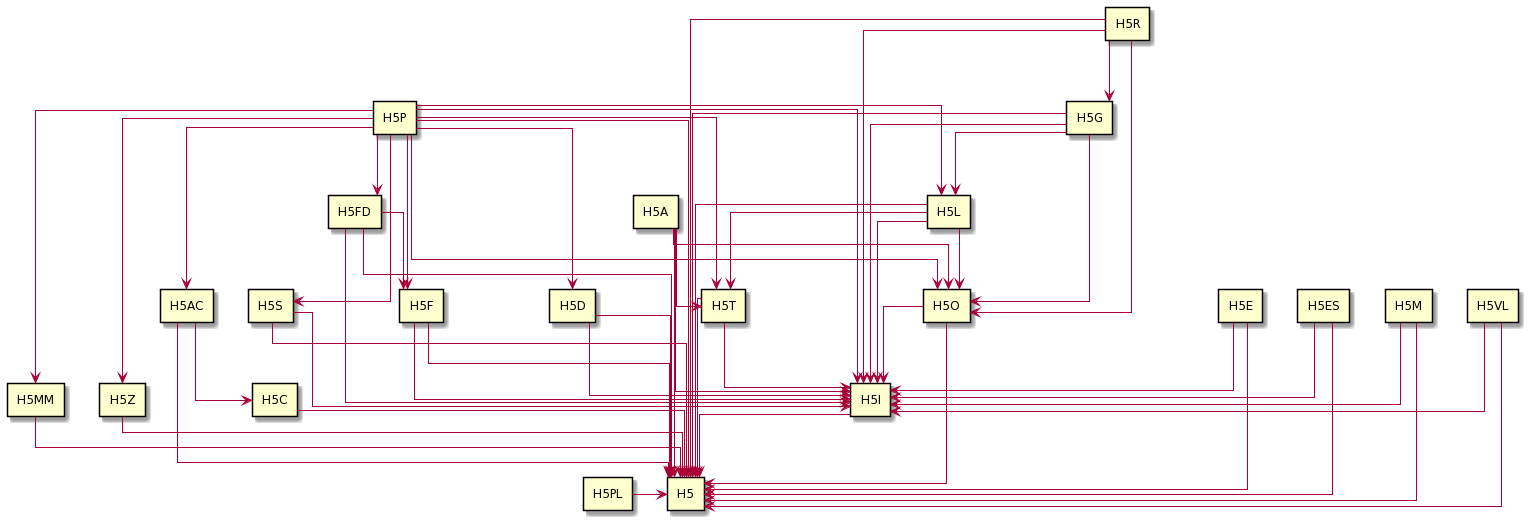
\includegraphics[scale=0.4,angle=90]{images/packackages-public-dependence.png}
\caption{The public dependence of HDF5 library modules as a directed graph.\label{fig:pub-module-dep}}
\end{sidewaysfigure}
\end{landscape}

% @startuml

% skin rose
% skinparam defaultFontSize 12
% skinparam backgroundColor transparent
% left to right direction

% rectangle "H5" {
%   rectangle public as h5public
% }
% package "H5A" {
%   rectangle public as h5apublic
%   rectangle private as h5aprivate
%   rectangle pkg as h5apkg
% }
% rectangle "H5B2" {
%   rectangle private as h5b2private
% }
% rectangle "H5FL" {
%   rectangle private as h5flprivate
% }
% rectangle "H5G" {
%   rectangle private as h5gprivate
% }
% rectangle "H5HF" {
%   rectangle private as h5hfprivate
% }
% rectangle "H5I" {
%   rectangle public as h5ipublic
% }
% rectangle "H5O" {
%   rectangle public as h5opublic
%   rectangle private as h5oprivate
% }
% rectangle "H5S" {
%   rectangle private as h5sprivate
% }
% rectangle "H5T" {
%   rectangle public as h5tpublic
%   rectangle private as h5tprivate
% }

% h5apublic --> h5public
% h5apublic --> h5ipublic
% h5apublic --> h5opublic
% h5apublic --> h5tpublic

% h5aprivate -[dashed]-> h5gprivate
% h5aprivate -[dashed]-> h5oprivate
% h5aprivate -[dashed]-> h5sprivate
% h5aprivate -[dashed]-> h5tprivate

% h5apkg -[dotted]-> h5b2private
% h5apkg -[dotted]-> h5flprivate
% h5apkg -[dotted]-> h5hfprivate
% h5apkg -[dotted]-> h5oprivate
% h5apkg -[dotted]-> h5sprivate
% h5apkg -[dotted]-> h5tprivate

% @enduml

\begin{figure}[!ht]
  \centering
  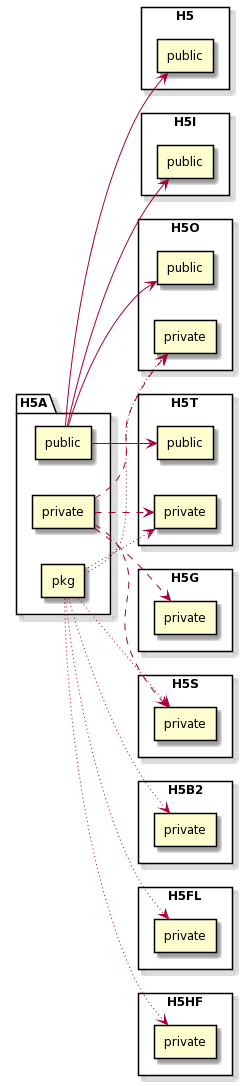
\includegraphics[scale=0.55]{images/H5A-dependence.png}
  \caption{\texttt{H5A} package dependence across visibilities.}
  \label{fig:h5a-dep}
\end{figure}

% \begin{table}
%   \centering
%  \caption{Internal package dependencies (in HDF5 1.14.3 - will change over time)}
% \label{table:mod-dep}
% {\tiny %
% \setlength\tabcolsep{2.25pt} % default value: 6pt
% \begin{tabular}{||c|c|c|c|c|c|c|c|c|c|c|c|c|c|c|c|c|c|c|c|c|c|c|c|c|c|c|c|c|c|c|c|c|c|c|c|c|c|c|c|c|c|c|c||}
% \hline
%   $\rightarrow$
%   & \texttt{A} & \texttt{AC} & \texttt{B} & \texttt{B2} & \texttt{C} & \texttt{CS} & \texttt{CX} & \texttt{D} & \texttt{E} &\texttt{EA}
%   & \texttt{ES} & \texttt{F} & \texttt{FA} & \texttt{FD} & \texttt{FL} & \texttt{FO} & \texttt{FS} & \texttt{G} & \texttt{H5} & \texttt{HF}
%   & \texttt{HG} & \texttt{HL} & \texttt{I} & \texttt{L} & \texttt{M} & \texttt{MF} & \texttt{MM} & \texttt{O} & \texttt{P} & \texttt{PB}
%   & \texttt{PL} & \texttt{R} & \texttt{RS} & \texttt{S} & \texttt{SL} & \texttt{SM} & \texttt{T} & \texttt{TS} & \texttt{UC} & \texttt{VL}
%   & \texttt{VM} & \texttt{WB} & \texttt{Z} \\ [0.5ex] 
% \hline\hline
% \texttt{A} & \textopenbullet & & & & & & \textbullet & & \textbullet & & \textbullet & & & & \textbullet & & & & \textbullet & & & & \textbullet & & & & \textbullet & \textbullet & & & & & & \textbullet & & & & & & \textbullet & & & \\ \hline
% \texttt{AC} & & \textopenbullet & & & \textbullet & & \textbullet & & \textbullet & & & \textbullet & & & & & & & \textbullet & & & & \textbullet & & & & \textbullet & & \textbullet & & & & & & \textbullet & & & & & & & & \\ \hline
% \texttt{B} & & & \textopenbullet & & & & \textbullet & & \textbullet & & & & & & & & & & \textbullet & & & & \textbullet & & & \textbullet & \textbullet & & \textbullet & & & & & & & & & & & & & & \\ \hline
% \texttt{B2} & & \textbullet & & \textopenbullet & & & & & \textbullet & & & \textbullet & & & \textbullet & & & \textopenbullet & \textbullet & & & & & & & \textbullet & \textbullet & & & & & & & & & & & & & & \textbullet & & \\ \hline
% \texttt{C} & & \textbullet & & & \textopenbullet & & \textbullet & & \textbullet & & & \textbullet & & \textbullet & \textbullet & & & & \textbullet & & & & & & & \textbullet & \textbullet & & & & & & & & & & & & & & \textbullet & & \\ \hline
% \texttt{CS} & & & & & & \textopenbullet & & & \textbullet & & & & & & & & & & \textbullet & & & & & & & & & & & & & & & & & & & & & & & & \\ \hline
% \texttt{CX} & & & & & & & \textopenbullet & \textbullet & \textbullet & & & & & & \textbullet & & & & \textbullet & & & & \textbullet & \textbullet & & & \textbullet & & \textbullet & & & & & & & & & & & & & & \\ \hline
% \texttt{D} & & \textbullet & \textbullet & & & & \textbullet & \textopenbullet & \textbullet & \textbullet & \textbullet & & \textbullet & \textbullet & \textbullet & \textbullet & & \textbullet & \textbullet & & \textbullet & \textbullet & \textbullet & \textbullet & & \textbullet & \textbullet & \textbullet & \textbullet & \textbullet & & & & \textbullet & & & & & & \textbullet & \textbullet & \textbullet & \\ \hline
% \texttt{E} & & & & & & & & & \textopenbullet & & & & & & \textbullet & & & & \textbullet & & & & \textbullet & & & & \textbullet &  & & & & & & & & & & \textbullet & & & & & \\ \hline
% \texttt{EA} & & & & & & & & & \textbullet & \textopenbullet & & & & & \textbullet & & & & \textbullet & & & & & & & \textbullet & \textbullet & & & & & & & & & & & & & & \textbullet & \textbullet & \\ \hline
% \texttt{ES} & & & & & & & & & \textbullet & & \textopenbullet & & & & \textbullet & & & & \textbullet & & & & & & & & \textbullet & & & & & & \textbullet & & & & & & & & & & \\ \hline
% \texttt{F} & & \textbullet & & & & & \textbullet & \textbullet & \textbullet & & \textbullet & \textopenbullet & & & \textbullet & \textbullet & & \textbullet & \textbullet & & \textbullet & & \textbullet & \textbullet & & \textbullet & \textbullet & \textbullet & \textbullet & \textbullet & & & & \textbullet & & \textbullet & \textbullet & & & \textbullet &  & & \\ \hline
% \texttt{FA} & & & & & & & & & \textbullet & & & & \textopenbullet & & \textbullet & & & & \textbullet & & & & & & & \textbullet & \textbullet & \textbullet & & & & & & & & & & & & & \textbullet & \textbullet & \\ \hline
% \texttt{FD} & & & & & & & \textbullet & \textbullet & \textbullet & & & \textbullet & & \textopenbullet & \textbullet & & & & \textbullet & & & & \textbullet & & & & \textbullet & & \textbullet & & \textbullet & & & & \textbullet & & & & & & & & \\ \hline
% \texttt{FL} & & & & & & \textbullet & & & \textbullet & & & & & & \textopenbullet & & & & \textbullet & & & & & & & & \textbullet &  & & & & & & & & & & & & & & & \\ \hline
% \texttt{FO} & & & & & & & & & \textbullet & & & \textbullet & & & \textbullet & \textopenbullet & & & \textbullet & & & & & & & & & \textbullet & & & & & & & & & & & & & & & \\ \hline
% \texttt{FS} & & \textbullet & & & & & & & \textbullet & & & \textbullet & & & & & \textopenbullet & & \textbullet & \textbullet & & & & & & \textbullet & \textbullet & & & & & & & & & & & & & & \textbullet & \textbullet & \\ \hline
% \texttt{G} & & \textbullet & & & & & \textbullet & \textbullet & \textbullet & & \textbullet & \textbullet & & & \textbullet & \textbullet & & \textopenbullet & \textbullet & & & \textbullet & \textbullet & \textbullet & & \textbullet & \textbullet & \textbullet & \textbullet & & & & & & \textbullet & & & & & \textbullet & & \textbullet & \\ \hline
% \texttt{H5} & & \textbullet & & & & & \textbullet & \textbullet & \textbullet & & & & & & \textbullet & & \textbullet & & \textopenbullet & & & & & \textbullet & & & \textbullet & & \textbullet & & \textbullet & & & & \textbullet & & \textbullet & & & & & & \\ \hline
% \texttt{HF} & & \textbullet & & \textbullet & & & & & \textbullet & & & \textbullet & & & \textbullet & \textbullet & & & \textbullet & \textopenbullet & & & & & & \textbullet & \textbullet & & & & & & & & & & & & & & \textbullet & \textbullet & \\ \hline
% \texttt{HG} & & \textbullet & & & & & & & \textbullet & & & \textbullet & & & & & & & \textbullet & & \textopenbullet & & \textbullet & & & \textbullet & \textbullet & & & & & & & & & & & & & & & & \\ \hline
% \texttt{HL} & & \textbullet & & & \textbullet & & & & \textbullet & & & \textbullet & & & \textbullet & & & & \textbullet & & & \textopenbullet & & & & \textbullet & \textbullet & & & & & & & & & & & & & & & & \\ \hline
% \texttt{I} & & & & & & & \textbullet & \textbullet & \textbullet & & & \textbullet & & & \textbullet & & & \textbullet & \textbullet & & & & \textopenbullet & & & & \textbullet & & \textbullet & & & & \textbullet & & & & \textbullet & & & \textbullet & & & \\ \hline
% \texttt{L} & & \textbullet & & & & & \textbullet & & \textbullet & & \textbullet & \textbullet & & & & & & \textbullet & \textbullet & & & & \textbullet & \textopenbullet & & & \textbullet & \textbullet & \textbullet & & & & & & & & & & & \textbullet & & & \\ \hline
% \texttt{M} & & & & & & & \textbullet & & \textbullet & & \textbullet & & & & & & & & \textbullet & & & & \textbullet & & \textopenbullet & & & & & & & & & & & & & & & \textbullet & & & \\ \hline
% \texttt{MF} & & & & & & & & & \textbullet & & & \textbullet & & & & & \textbullet & & \textbullet & & & & \textbullet & & & \textopenbullet & & & & & & & & & & & & & & & \textbullet & & \\ \hline
% \texttt{MM} & & & & & & & & & \textbullet & & & & & & & & & & \textbullet & & & & & & & & \textopenbullet & & & & & & & & & & & & & & & & \\ \hline
% \texttt{O} & \textbullet & \textbullet & & & & & \textbullet & \textbullet & \textbullet & & \textbullet & \textbullet & & & \textbullet & \textbullet & & \textbullet & \textbullet & \textbullet & \textbullet & \textbullet & \textbullet & \textbullet & & \textbullet & \textbullet & \textopenbullet & \textbullet & & & \textbullet & & \textbullet & & \textbullet & \textbullet & & & \textbullet & \textbullet & \textbullet & \textbullet \\ \hline
% \texttt{P} & & \textbullet & \textbullet & & & & \textbullet & \textbullet & \textbullet & & & \textbullet & & \textbullet & \textbullet & & & \textbullet & \textbullet & & & & \textbullet & \textbullet & \textbullet & & \textbullet & \textbullet & \textopenbullet & & & & & \textbullet & & & \textbullet & & & \textbullet & \textbullet & & \textbullet \\ \hline
% \texttt{PB} & & & & & & & & & \textbullet & & & \textbullet & & \textbullet & & & & & \textbullet & & & & \textbullet & & & & \textbullet & & & \textopenbullet & & & & & \textbullet & & & & & & & & \\ \hline
% \texttt{PL} & & & & & & & & & \textbullet & & & & & & & & & & \textbullet & & & & & & & & \textbullet & & & & \textopenbullet & & & & & & & & & & & & \textbullet \\ \hline
% \texttt{R} & & & & & & & \textbullet & & \textbullet & & & & & & & & & & \textbullet & & & & \textbullet & & & & \textbullet & & & & & \textopenbullet & & \textbullet & & & & & & \textbullet & & & \\ \hline
% \texttt{RS} & & & & & & & & & \textbullet & & & & & & \textbullet & & & & \textbullet & & & & & & & & & & & & & & \textopenbullet & & & & & & & & & & \\ \hline
% \texttt{S} & & & & & & & \textbullet & \textbullet & \textbullet & & & \textbullet & & & \textbullet & & & & \textbullet & & & & \textbullet & & & & \textbullet & \textbullet & & & & & & \textopenbullet & & & & & & & \textbullet & & \\ \hline
% \texttt{SL} & & & & & & & & & \textbullet & & & & & & \textbullet & & & & \textbullet & & & & & & & & \textbullet & & & & & & & & \textopenbullet & & & & & & & & \\ \hline
% \texttt{SM} & & \textbullet & & & & & & & \textbullet & & & \textbullet &  & & \textbullet & & & & \textbullet & & & & & & & \textbullet & \textbullet & \textbullet & & & & & & & & \textopenbullet & & & & & & \textbullet & \\ \hline
% \texttt{T} & & \textbullet & & & & & \textbullet & \textbullet & \textbullet & & \textbullet & \textbullet & & & \textbullet & \textbullet & & \textbullet & \textbullet & & & & \textbullet & \textbullet & & & \textbullet & \textbullet & \textbullet & & & \textbullet & & & & & \textopenbullet & & & \textbullet & & \textbullet & \\ \hline
% \texttt{TS} & & & & & & & & & \textbullet & & & & & & & & & & \textbullet & & & & & & & & \textbullet & & & & & & & & & & & \textopenbullet & & & & & \\ \hline
% \texttt{UC} & & & & & & & & & \textbullet & & & & & & \textbullet & & & & & & & & & & & & & & & & & & & & & & & & \textopenbullet & & & & \\ \hline
% \texttt{VL} & \textbullet & \textbullet & & & \textbullet & & \textbullet & \textbullet & \textbullet & & \textbullet & \textbullet & & & \textbullet & & & \textbullet & \textbullet & & \textbullet & & \textbullet & \textbullet & \textbullet & \textbullet & \textbullet & \textbullet & \textbullet & \textbullet & \textbullet & & & \textbullet & \textbullet & & \textbullet & & & \textopenbullet & & & \\ \hline
% \texttt{VM} & & & & & & & & & \textbullet & & & & & & & & & & \textbullet & & & & & & & & \textbullet & \textbullet & & & & & & & & & & & & & \textopenbullet & & \\ \hline
% \texttt{WB} & & & & & & & & & \textbullet & & & & & & \textbullet & & & & \textbullet & & & & & & & & & & & & & & & & & & & & & & & \textopenbullet & \\ \hline
% \texttt{Z} & & & & & & & \textbullet & \textbullet & \textbullet & & & \textbullet & & & & & & & \textbullet & & & & \textbullet & & & & \textbullet & \textbullet & \textbullet & & \textbullet & & & \textbullet & & & & & & & & & \textopenbullet \\
% \hline
% \end{tabular}
% }%
% \end{table}

\chapter{Feature chronology}\label{app:chronology}
%CLEANUP \todo[inline]{Owner: Dana -- Priority: Medium -- Effort: S -- Completion: 5\%}
\begin{center}
\begin{tabular}{|c|l|}
\hline 
\textbf{Version}~~~~ & \textbf{Major Feature Introduction}\tabularnewline
\hline 
\hline 
\multirow{3}{*}{1.8.0} & External links\tabularnewline
\cline{2-2} 
 & Non-persistent free-space tracking\tabularnewline
\cline{2-2} 
 & Unlimited attribute size\tabularnewline
\hline 
1.8.5 & Group compression\tabularnewline
\hline 
\multirow{3}{*}{1.10.0} & Single-Writer Multiple Reader (SWMR)\tabularnewline
\cline{2-2} 
 & Virtual Datasets (VDS)\tabularnewline
\cline{2-2} 
 & 64-bit \texttt{hid\_t}\tabularnewline
\hline 
1.10.1 & Paged allocation and persistent free space tracking\tabularnewline
\hline 
1.10.2 & Parallel compression\tabularnewline
\hline 
1.12.0 & Virtual Object Layer (VOL)\tabularnewline
\hline 
\multirow{4}{*}{1.14.0} & Multi-dataset I/O\tabularnewline
\cline{2-2} 
 & Selection I/O\tabularnewline
\cline{2-2} 
 & Overhaul of VOL \tabularnewline
\cline{2-2} 
 & Subfiling VFD\tabularnewline
\hline 
\end{tabular}
\end{center}

\chapter{Feature (in-)compatibility}\label{app:feat-compat}
\todo[inline]{Owner: Dana -- Priority: High -- Effort: M -- Completion: 5\%}

\section{Operating Systems}

\subsection{Windows}
\begin{itemize}
    \item SWMR should work on Windows with local file systems (NOT SMB shares), though testing is not a robust as on MacOS/Linux
    \item Parallel HDF5 is poorly tested on Windows
    \item The direct VFD is not supported as it uses the POSIX \texttt{O\_DIRECT} flag
    \item Thread-safety uses win32 threads
    \item Some API calls use \texttt{off\_t}, which is 32-bits on Windows (we use \texttt{\_\_int64} internally)
    \item Unicode file paths are not well-supported
\end{itemize}

\section{Build Systems}

All features should be supported in both the Autotools and CMake.

\section{Feature Compatibility}

Only incompatibilities are noted (an empty cell implies compatibility).

\begin{minipage}{\textwidth}
  \begin{center}
    \begin{tabular}{|| c | c | c | c ||}
      \hline
      Feature & Serial & SWMR (serial) & Parallel \\
      \hline
      Free-space tracking & ? & ? & ?\\
      \hline
      Paged Allocation & ? & ? & ? \\
      \hline

      Virtual Dataset (VDS) Layout & ? & ? & ? \\
      \hline
      Variable-length datatypes & ? & ? & ? \\
      \hline
    \end{tabular}
  \end{center}
\end{minipage}

\section{Other Miscellaneous Limitations}
\begin{itemize}
    \item The current implementation of virtual datasets doesn't support point selections
    \item The direct VFD requires \texttt{open(2)} to take the \texttt{O\_DIRECT} flag
\end{itemize}

%\begin{minipage}{\textwidth}
%  \begin{center}
%    \begin{tabular}{|| c | c | c | c | c | c ||}
%      \hline
%      & SWMR & Paged Allocation & Free-space tracking & VDS & Non-fixed-size datatypes \\
%      \hline
%      SWMR & S & S? & S? & S & $\times$ \\
%      \hline
%      Paged Allocation & & P\footnote{No page buffering?} & P? & P? & S \\
%      \hline
%      Free-space tracking & & & P? & P? & S \\
%      \hline
%      VDS & & & & P & S \\
%      \hline
%      Non-fixed-size datatypes & & & & &  S \\
%      \hline
%    \end{tabular}
%  \end{center}
%\end{minipage}

%\paragraph{Symbology}
%\todo[inline]{GH: Is this a good way of breaking it down?}
%\begin{itemize}
%    \item S - sequential only
%    \item P - MPI parallel \& sequential
%    \item $\times$ - unsupported
%\end{itemize}

%\paragraph{Other}
%\begin{itemize}
%    \item The current implementation of virtual datasets doesn't support point selections
%\end{itemize}

% Other row/column candidates
% - VDS
% - Paged allocation/page buffering
% - ???

% Wrappers/High-level*
%Parallel vs. \\ Serial & Thread-Safe vs. \\ Not Thread-Safe & Windows/MacOS/ \\ Linux/Misc. POSIX \\
% https://stackoverflow.com/questions/2888817/footnotes-for-tables-in-latex for footnotes in table
% SWMR doesn't support variable-length and region reference datatypes

% Collective metadata writes aren't supported with page buffering, separate table probably(?)
% Page buffering doesn't support parallel HDF5

% Free space mangement

% ROS3 VFD -> 
% Lots of missing documentation

% Direct VFD

% Core, Direct, Onion, Family, Log, MPIO, Multi, Sec2, Splitter, Mirror, etc VFDs? 

% Metadata cache?

% 

\paragraph{VFD stackability and features}
\begin{center}
    \begin{tabular}{|| c | c ||}
      \hline
      \rotatebox{90}{Pass-Through} & family, mirror, multi/split, onion, splitter, subfiling \\
      \hline
      \rotatebox{90}{Terminal} & core, direct, HDFS, Hermes, log, MPI-I/O, sec2, ros3, stdio\\
      \hline
    \end{tabular}
  \end{center}

NOTE: The onion and subfiling VFDs are currently hard-coded to use the sec2 VFD.

\paragraph{VOL connector stackability}

\chapter{Environment}\label{app:environment}
\todo[inline]{Owner: Gerd -- Priority: High -- Effort: S -- Completion: 80\%}

What you need to follow along:

\begin{itemize}
    \item HDF5 library source code~\cite{libhdf52023}
    \item GCC~\cite{gcc2023} (compile stuff w/ \texttt{-g})
    \item Valgrind~\cite{valgrind2023}
    \item KCachegrind~\cite{kcachegrind2023}
    \item CMake~\cite{cmake2023}
    \item Clone the GitHub repository~\cite{hdf5-tourist}
\end{itemize}

\begin{minted}{shell}
# run the program with callgrind; generates a file callgrind.out.XYZUV
valgrind --tool=callgrind ./executable

# open profile.callgrind with kcachegrind
kcachegrind callgrind.out.XYZUV
\end{minted}

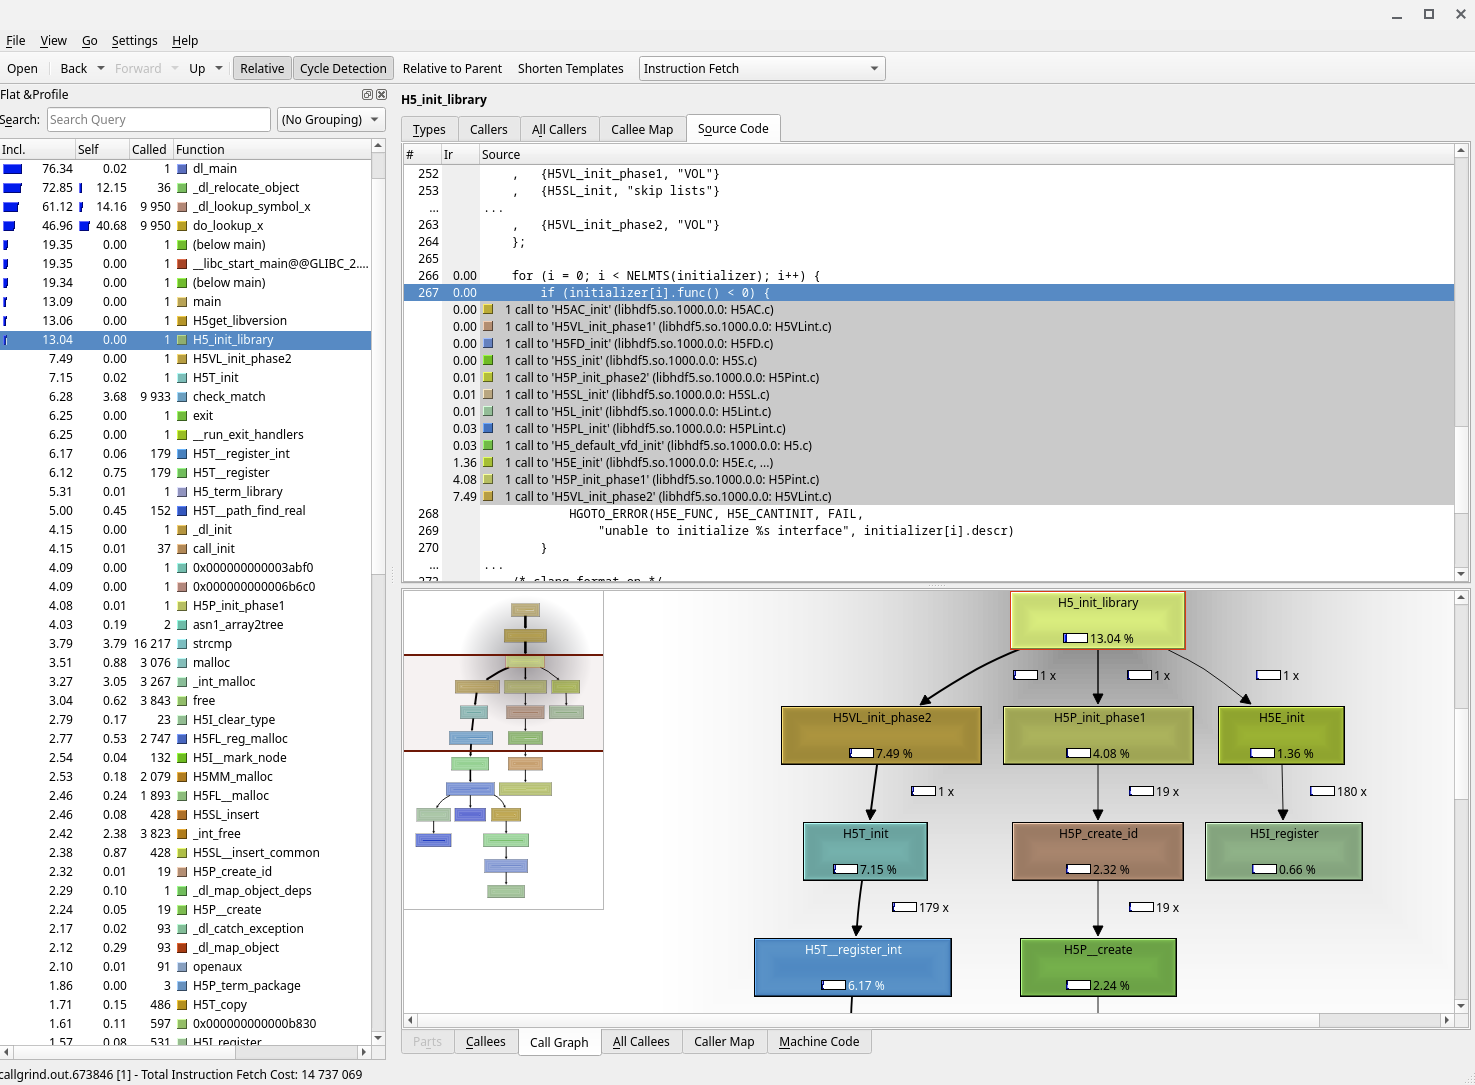
\includegraphics[scale=0.3]{images/kcachegrind.png}

Ease of navigation\ldots, but don't be fooled by pictures! You must look at the code.

\begin{figure}
\centering
\caption{Caption}
\label{fig:label1}
\begin{minted}[linenos]{C}
    ...
    struct {
        herr_t (*func)(void);
        const char *descr;
    } initializer[] = {
        {H5E_init, "error"}
    ,   {H5VL_init_phase1, "VOL"}
    ,   {H5SL_init, "skip lists"}
    ,   {H5FD_init, "VFD"}
    ,   {H5_default_vfd_init, "default VFD"}
    ,   {H5P_init_phase1, "property list"}
    ,   {H5AC_init, "metadata caching"}
    ,   {H5L_init, "link"}
    ,   {H5S_init, "dataspace"}
    ,   {H5PL_init, "plugins"}
    /* Finish initializing interfaces that depend on the interfaces above */
    ,   {H5P_init_phase2, "property list"}
    ,   {H5VL_init_phase2, "VOL"}
    };

    for (i = 0; i < NELMTS(initializer); i++) {
        if (initializer[i].func() < 0) {
            HGOTO_ERROR(H5E_FUNC, H5E_CANTINIT, FAIL,
                "unable to initialize %s interface", initializer[i].descr)
        }
    }
    ...
\end{minted}
\end{figure}

%\chapter{Stories}\label{app:stories}
%\subsection{Handles and property management}\label{sec:handles}

Most application developers experience the HDF5 library through handles (identifiers) and property lists. In this section, we present the essentials of how these primitives are managed internally in the library.

\begin{itemize}
    \item Identifier types and management
    \item Identifier life cycle
    \item VOL use of identifiers
    \item User-defined identifier types
\end{itemize}

\subsection{Property management}\label{sec:properties}

\begin{itemize}
    \item Property lists, property list classes, default properties, inheritance
    \item User-defined props.
\end{itemize}


\subsection{Library state}\label{sec:lib-state}

\todo{Neil will take care of this. Scot for Fortran-specific considerations?}

In this section, we describe the \textit{cross-cutting} infrastructure the library maintains for efficient operation, including certain global variables, API context, free lists, etc.

\begin{itemize}
    \item Default context, global data xfer property list cache
    \item ???
\end{itemize}

\subsection{Extension interfaces}

\todo{Jordan is the man.}

One of the values of HDF5 library development is extensibility. In this section, describe the architecture of four important extension interfaces, including the virtual object layer (VOL), filter plugins, and user-defined identifiers and links. The emphasis of this section is not on the development of such extensions, but on how they connect and integrate with library internals.

\begin{itemize}
    \item VOL connectors
    \item VFL plugins
    \item Filter plugins
    \item User-defined links
    \item User-defined datatype conversions
    \item Custom memory management (?)
    \item Iterator callbacks (?)
\end{itemize}

Other important extension interfaces are covered below, including the virtual file layer (VFL) in section~\ref{sec:vfl} and datatype conversions in section~\ref{sec:dtype-conv}.


\printbibliography

\end{document}